
\section{$k$-EXPTIME/$_{\raise.17ex\hbox{$\scriptstyle\sim$}}$}

\begin{frame}

\begin{compactenum}[$\bullet$]
\item<1-> Belongs to Descriptive Complexity
\item<2-> First contributor is R. Fagin (1974)
\item<3-> $\exists$SO captures NP
\end{compactenum}

\vspace{0.3cm}
\onslide<4-> Here
\begin{compactenum}[$\bullet$]
\item<4-> PHFL$^k$ captures $k$-EXPTIME/$_{\raise.17ex\hbox{$\scriptstyle\sim$}}$ over finite LTS
\item<4-> PHFL$^{k+1}_{tail}$ captures $k$-EXPSPACE/$_{\raise.17ex\hbox{$\scriptstyle\sim$}}$ over finite LTS
\end{compactenum}

\vspace{0.3cm}
\onslide<5->For EXPTIME it holds
\begin{compactenum}[$\bullet$]
\item<5-> $k=0$ was shown by M. Otto
\item<5-> $k=1$ was shown by E. Lozes and M. Lange
\end{compactenum}

\vspace{0.3cm}
\onslide<6->For EXPSPACE it holds
\begin{compactenum}[$\bullet$]
\item<6-> $k=0$ was shown by E. Lozes and M. Lange
\end{compactenum}

\end{frame}
\begin{frame}

Bisimulation-invariant Complexity Class

\begin{figure}[ht]
	\centering{
  \only<1>{\hspace{-0.1cm}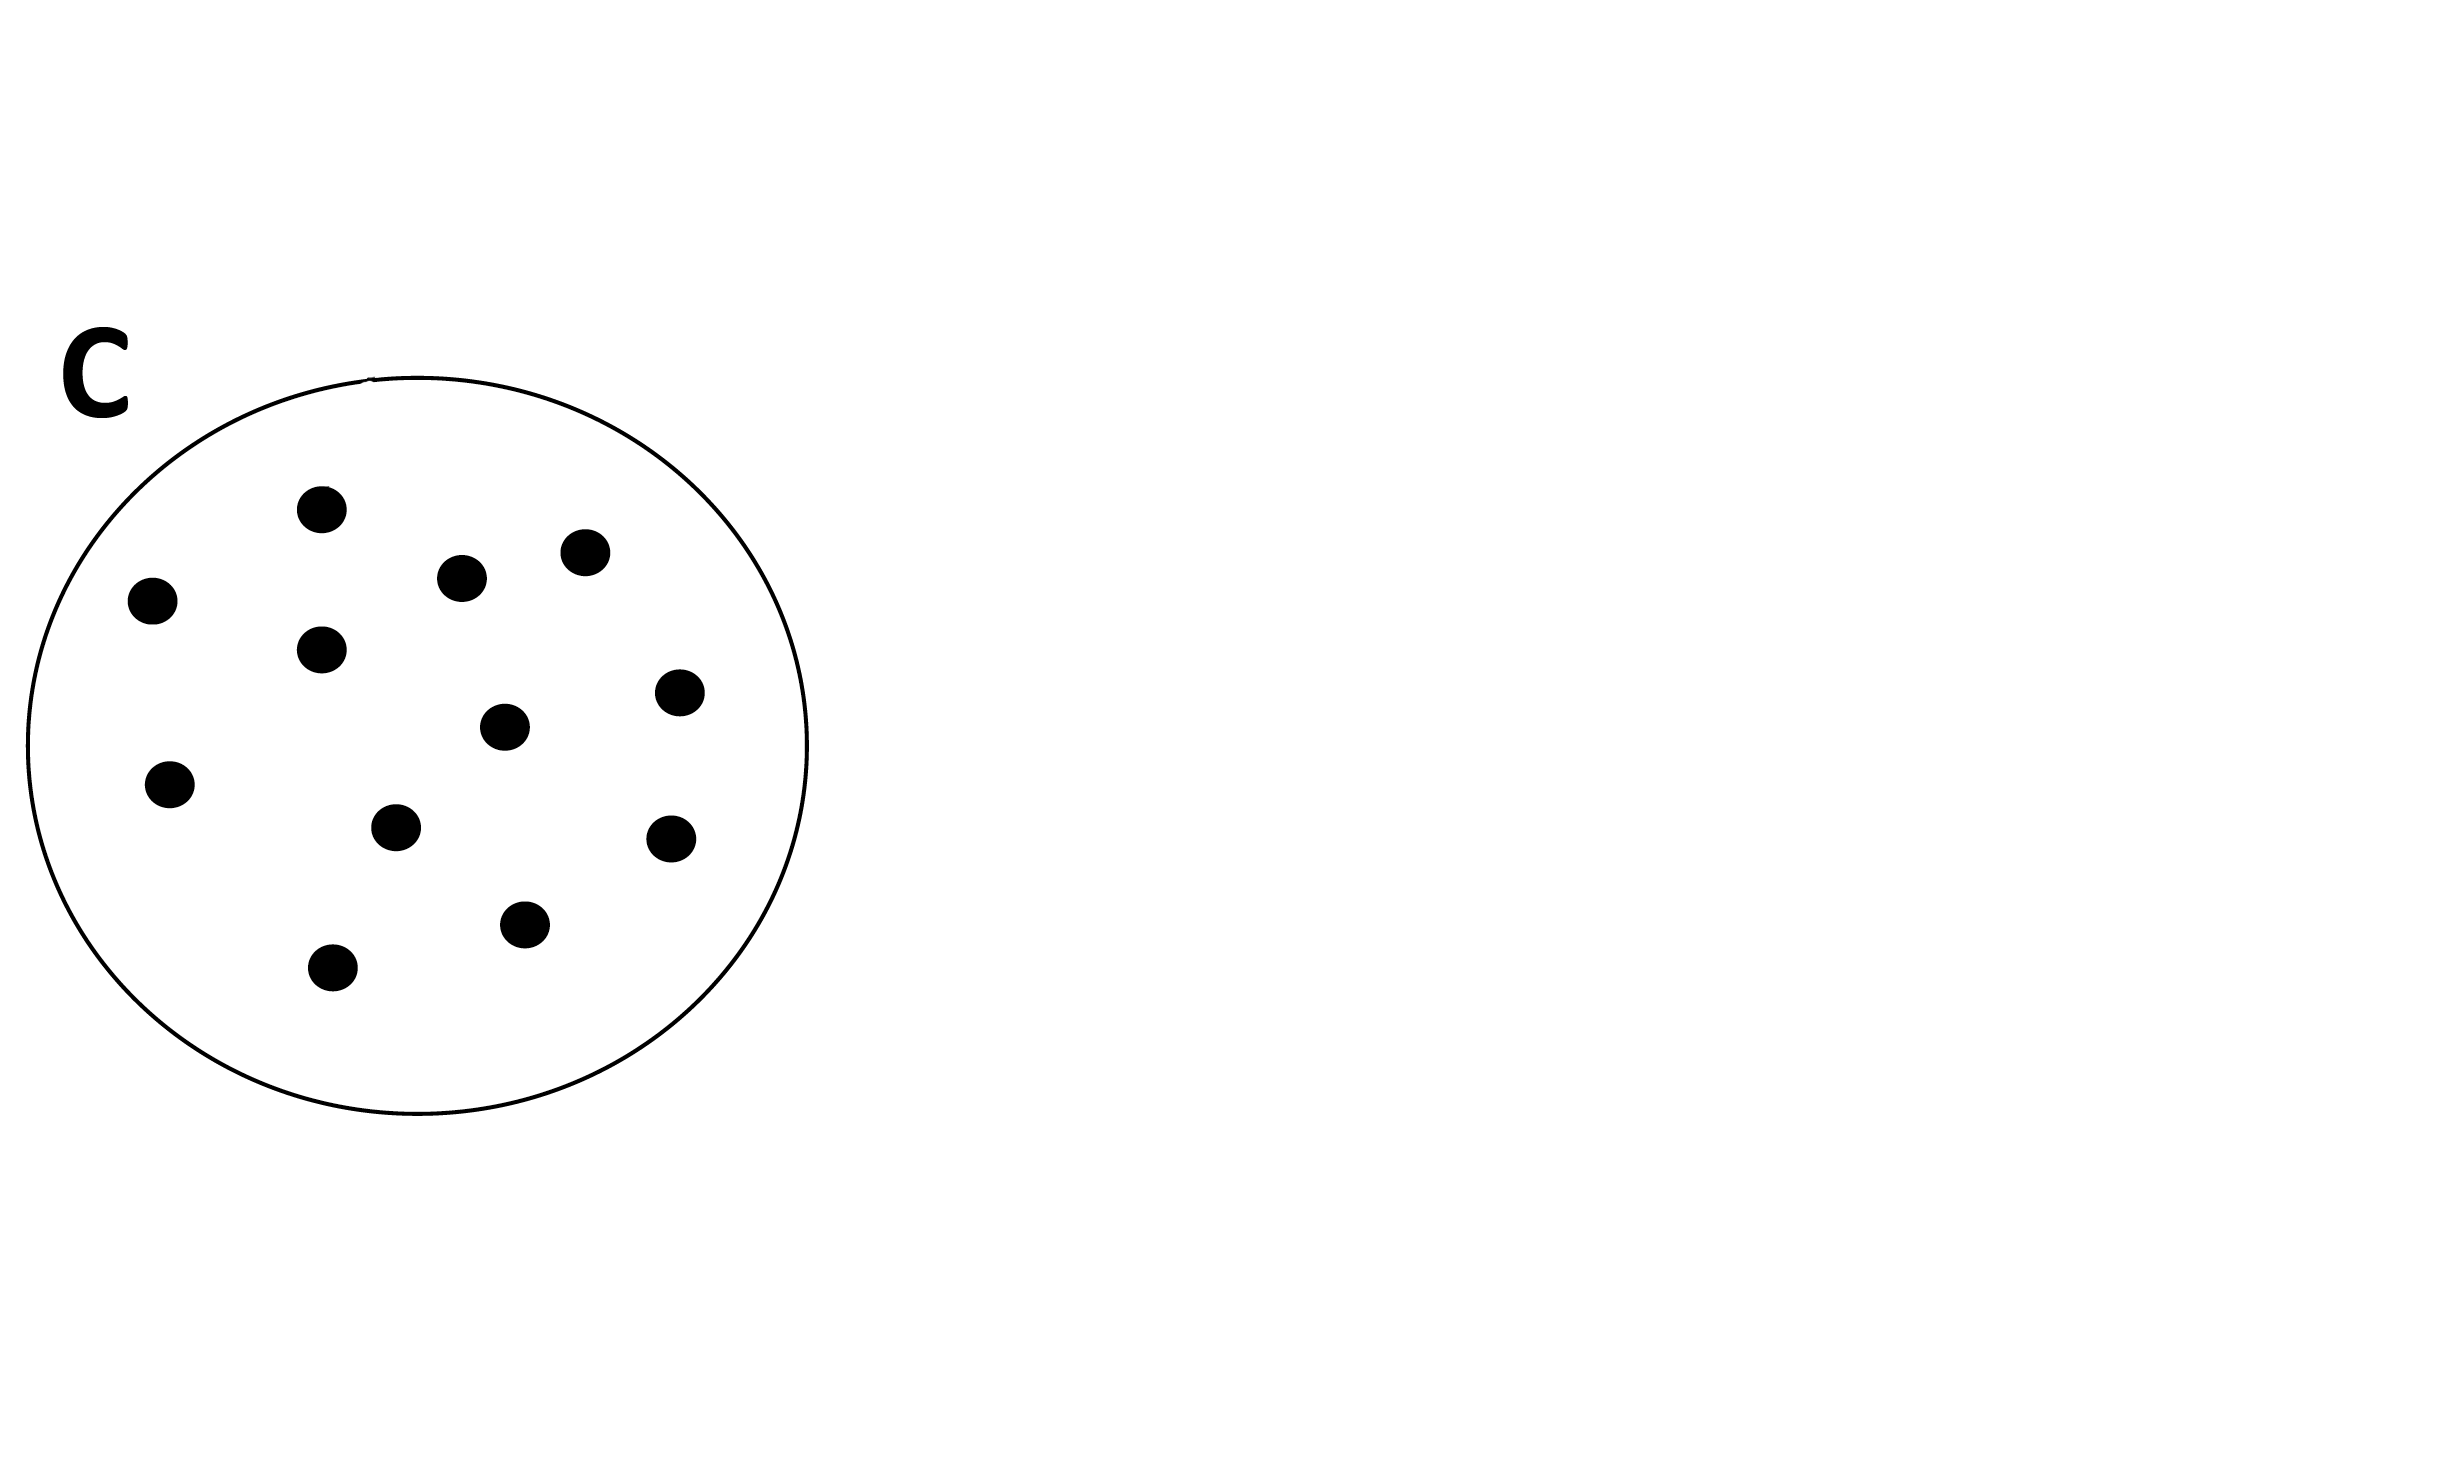
\includegraphics[width=0.9\textwidth]{bisimulation-invariant_0.png}}
  \only<2>{\hspace{-0.1cm}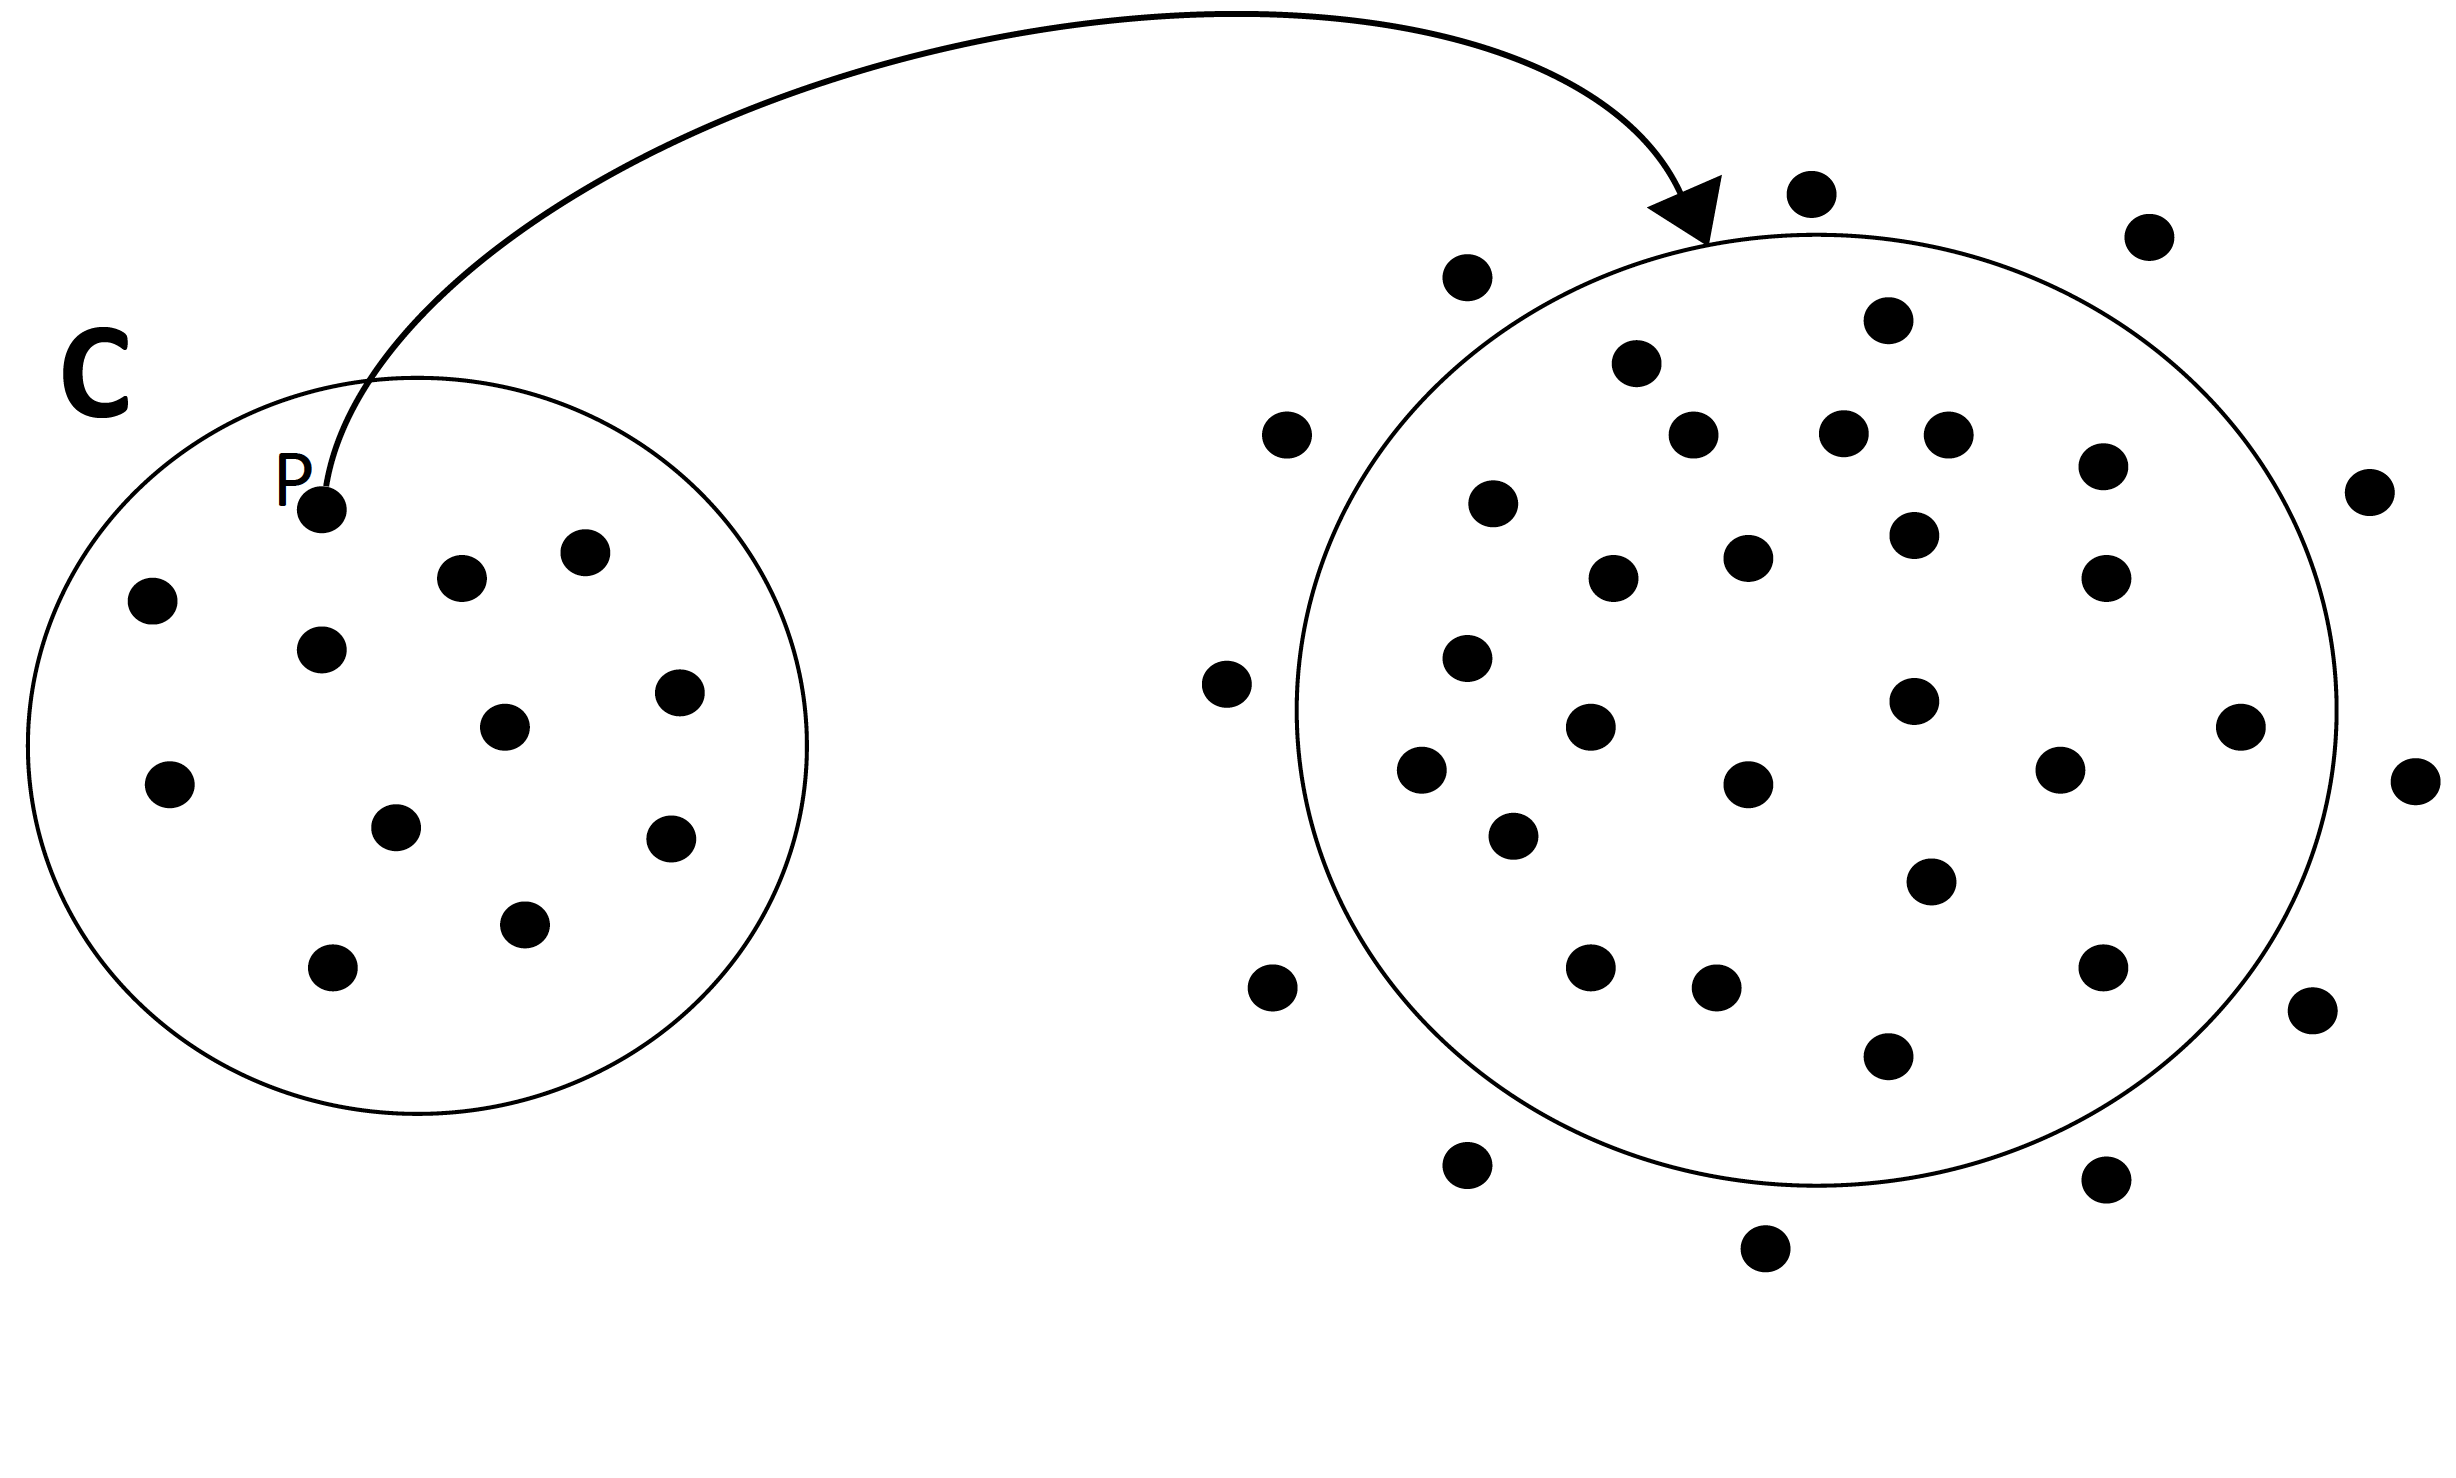
\includegraphics[width=0.9\textwidth]{bisimulation-invariant_1.png}}
  \only<3>{\hspace{-0.2cm}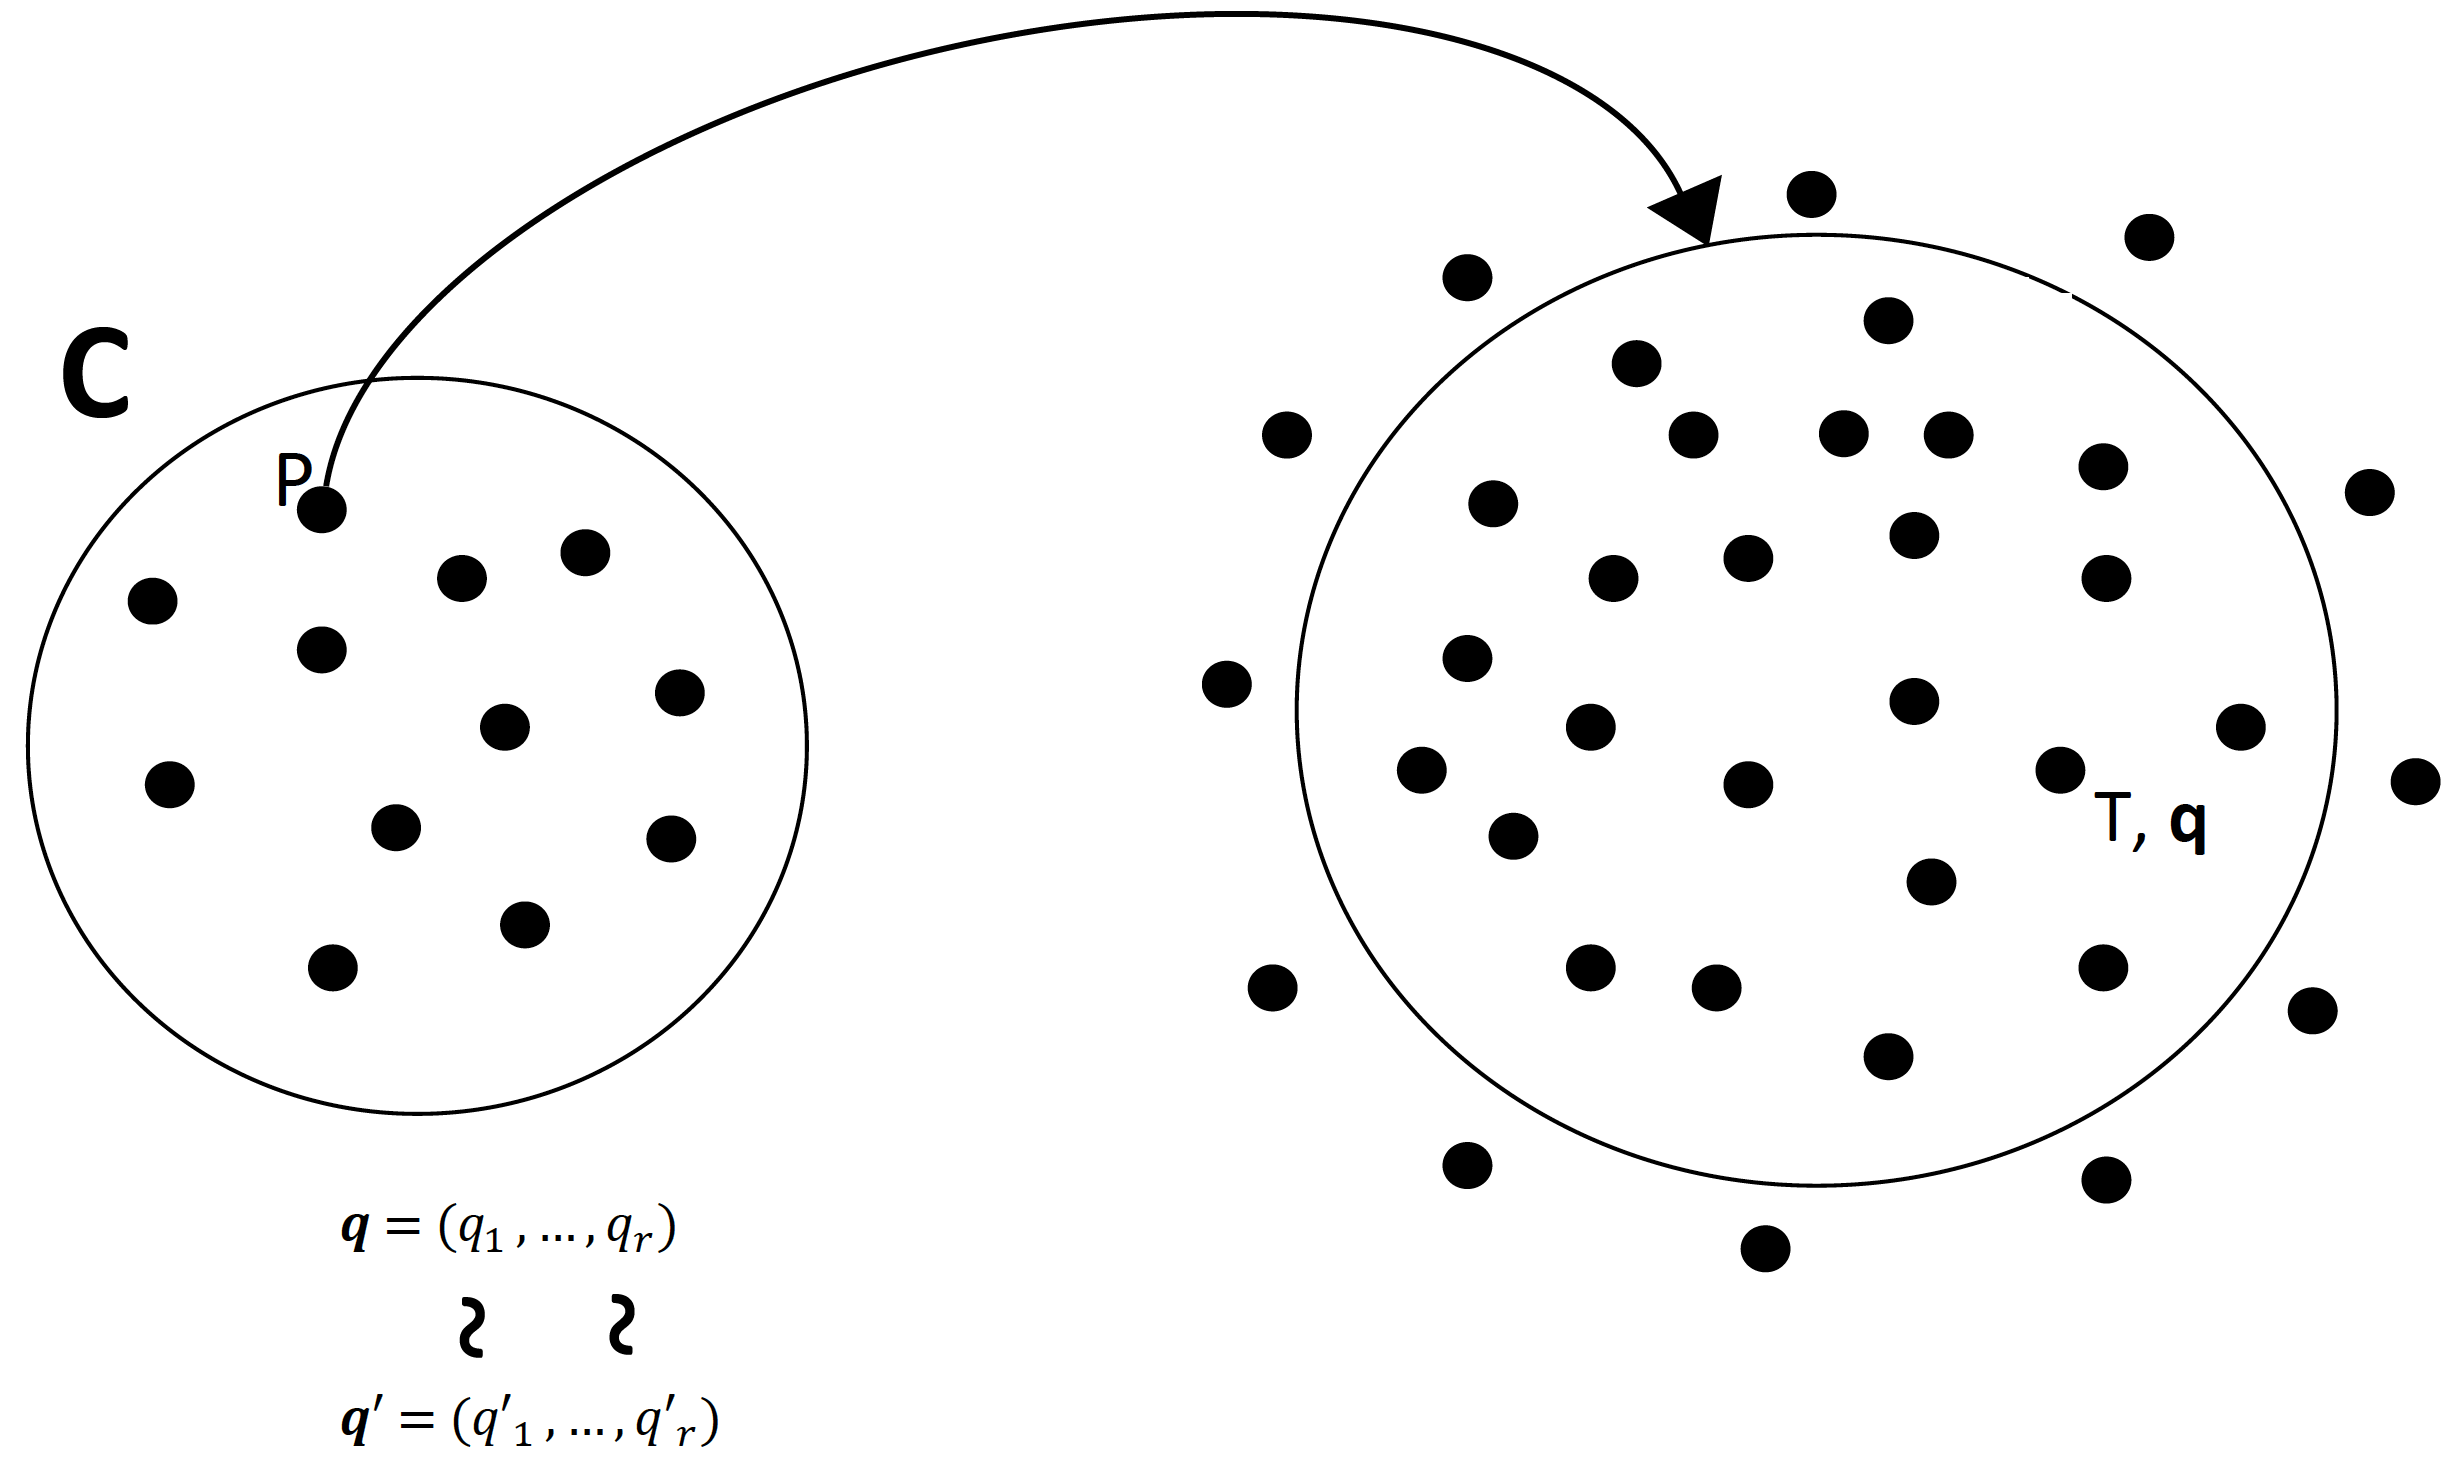
\includegraphics[width=0.9\textwidth]{bisimulation-invariant_2.png}}
  \only<4>{\hspace{-0.3cm}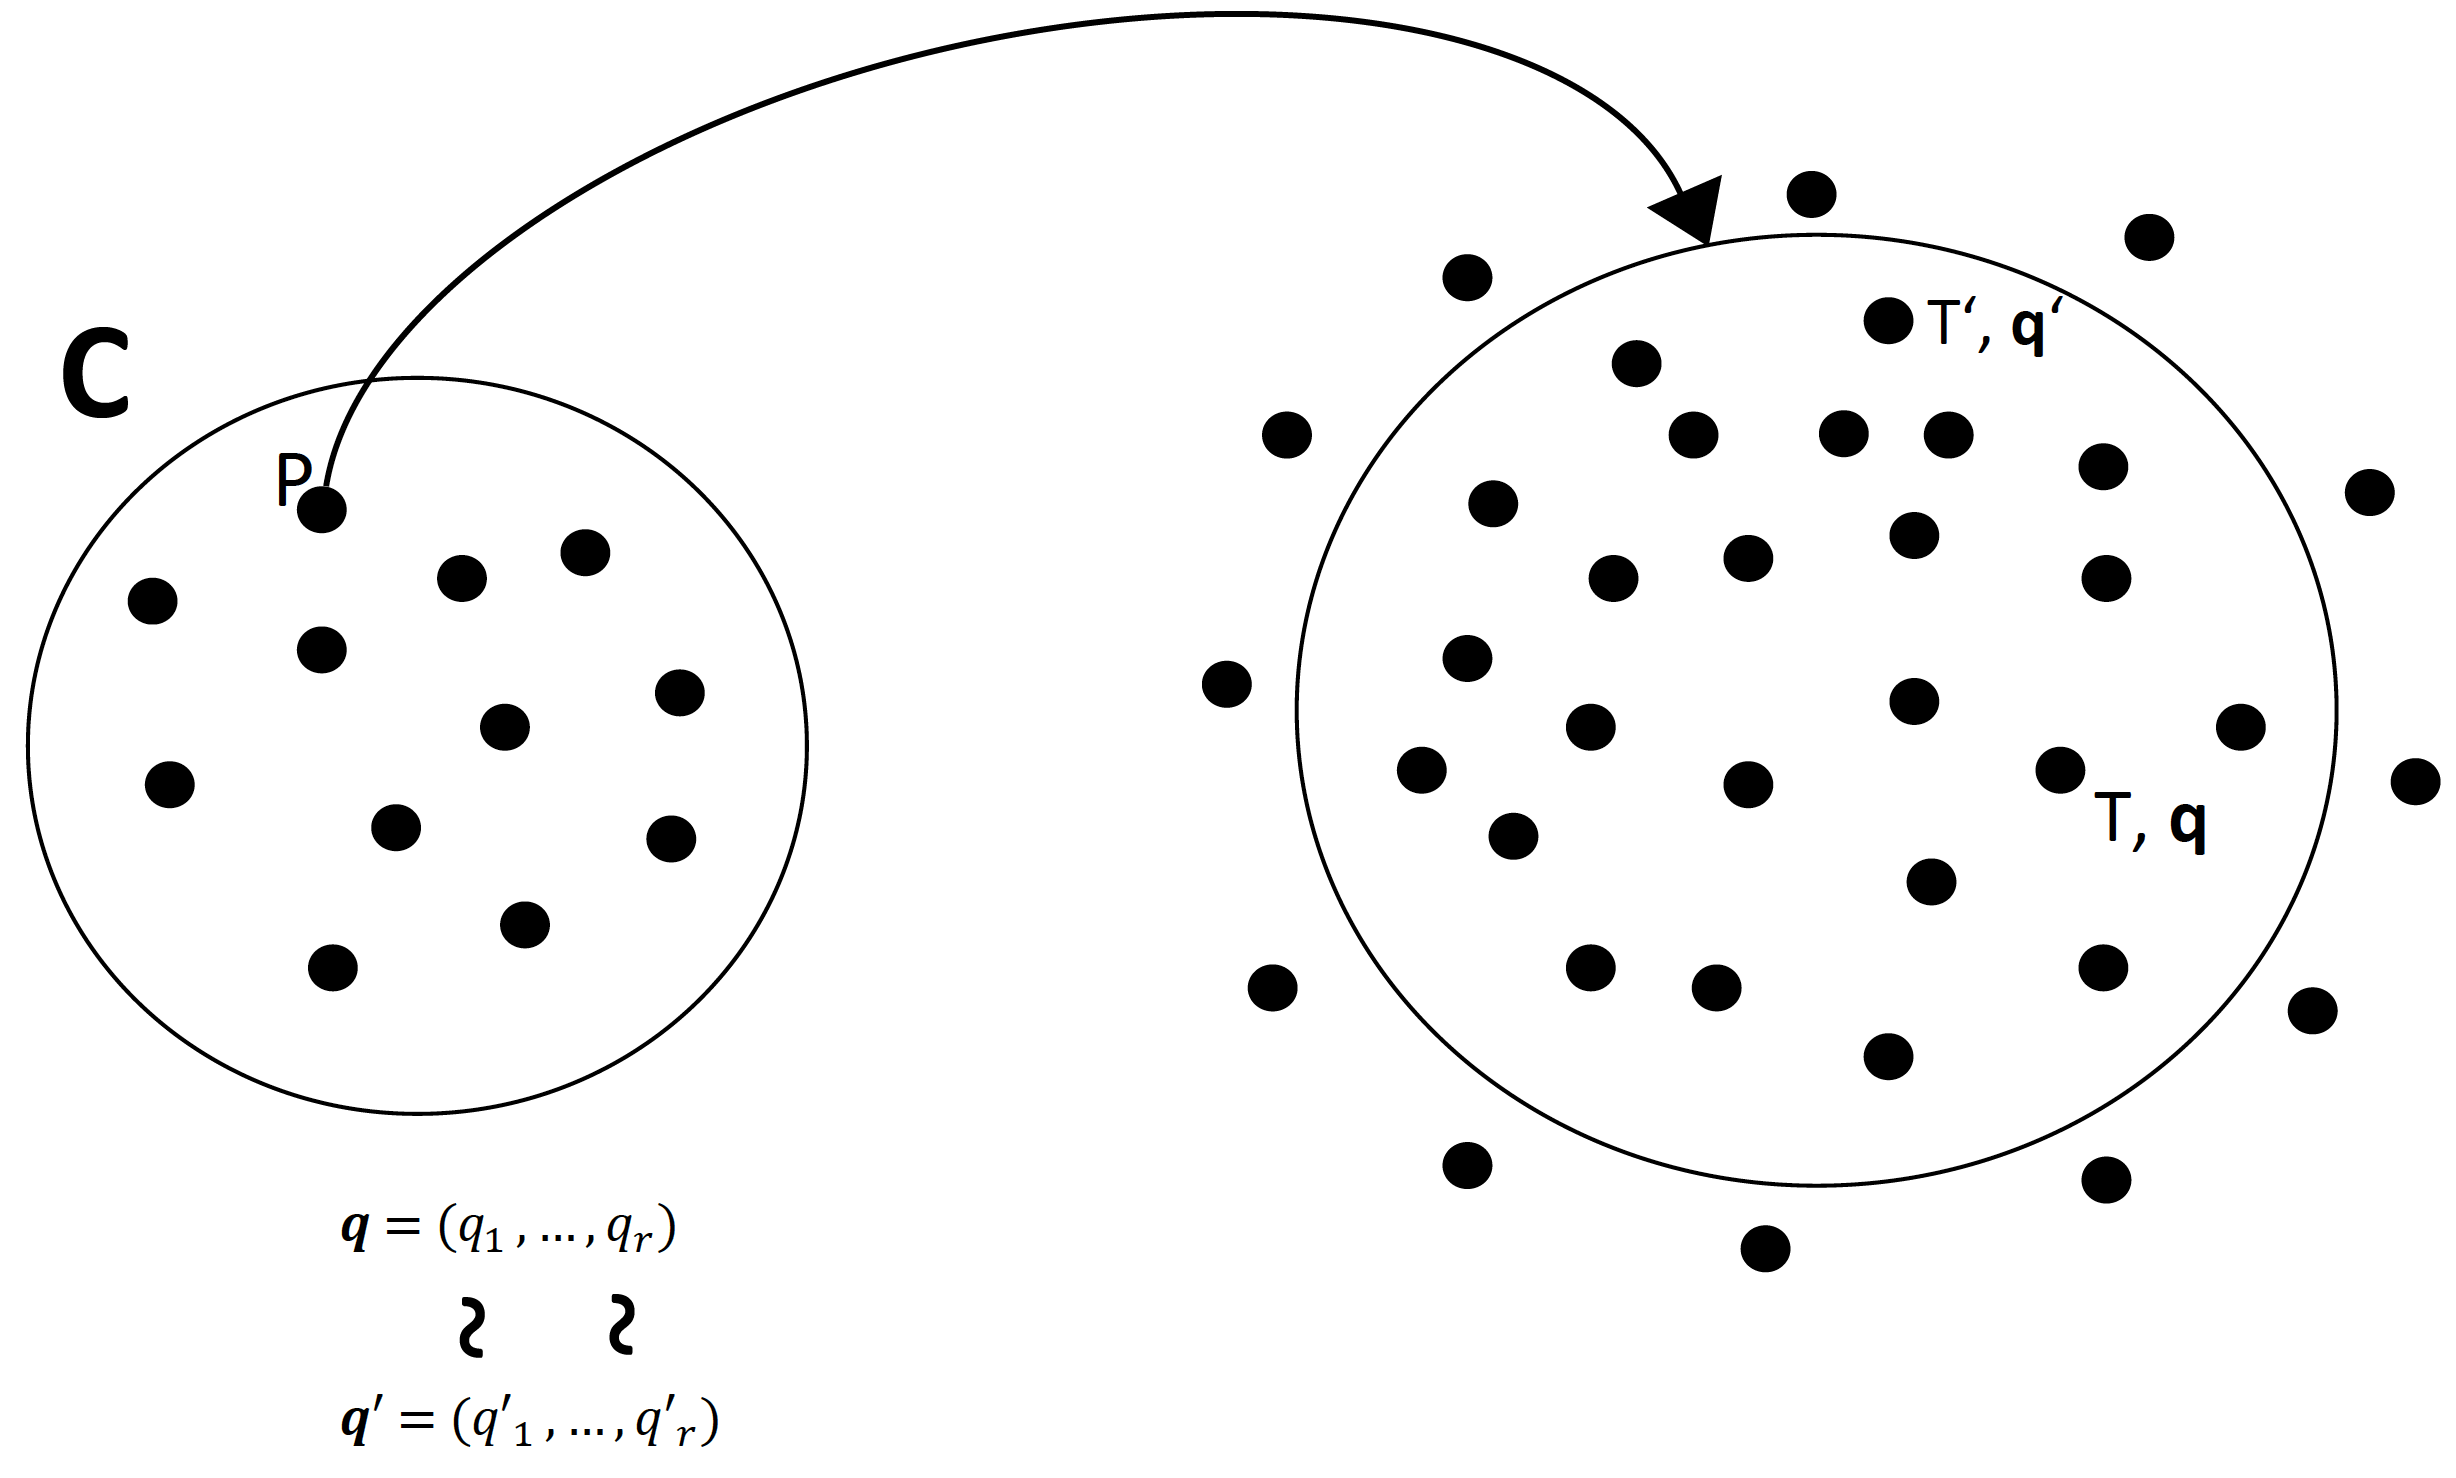
\includegraphics[width=0.9\textwidth]{bisimulation-invariant_3.png}}
  \only<5>{\hspace{-0.4cm}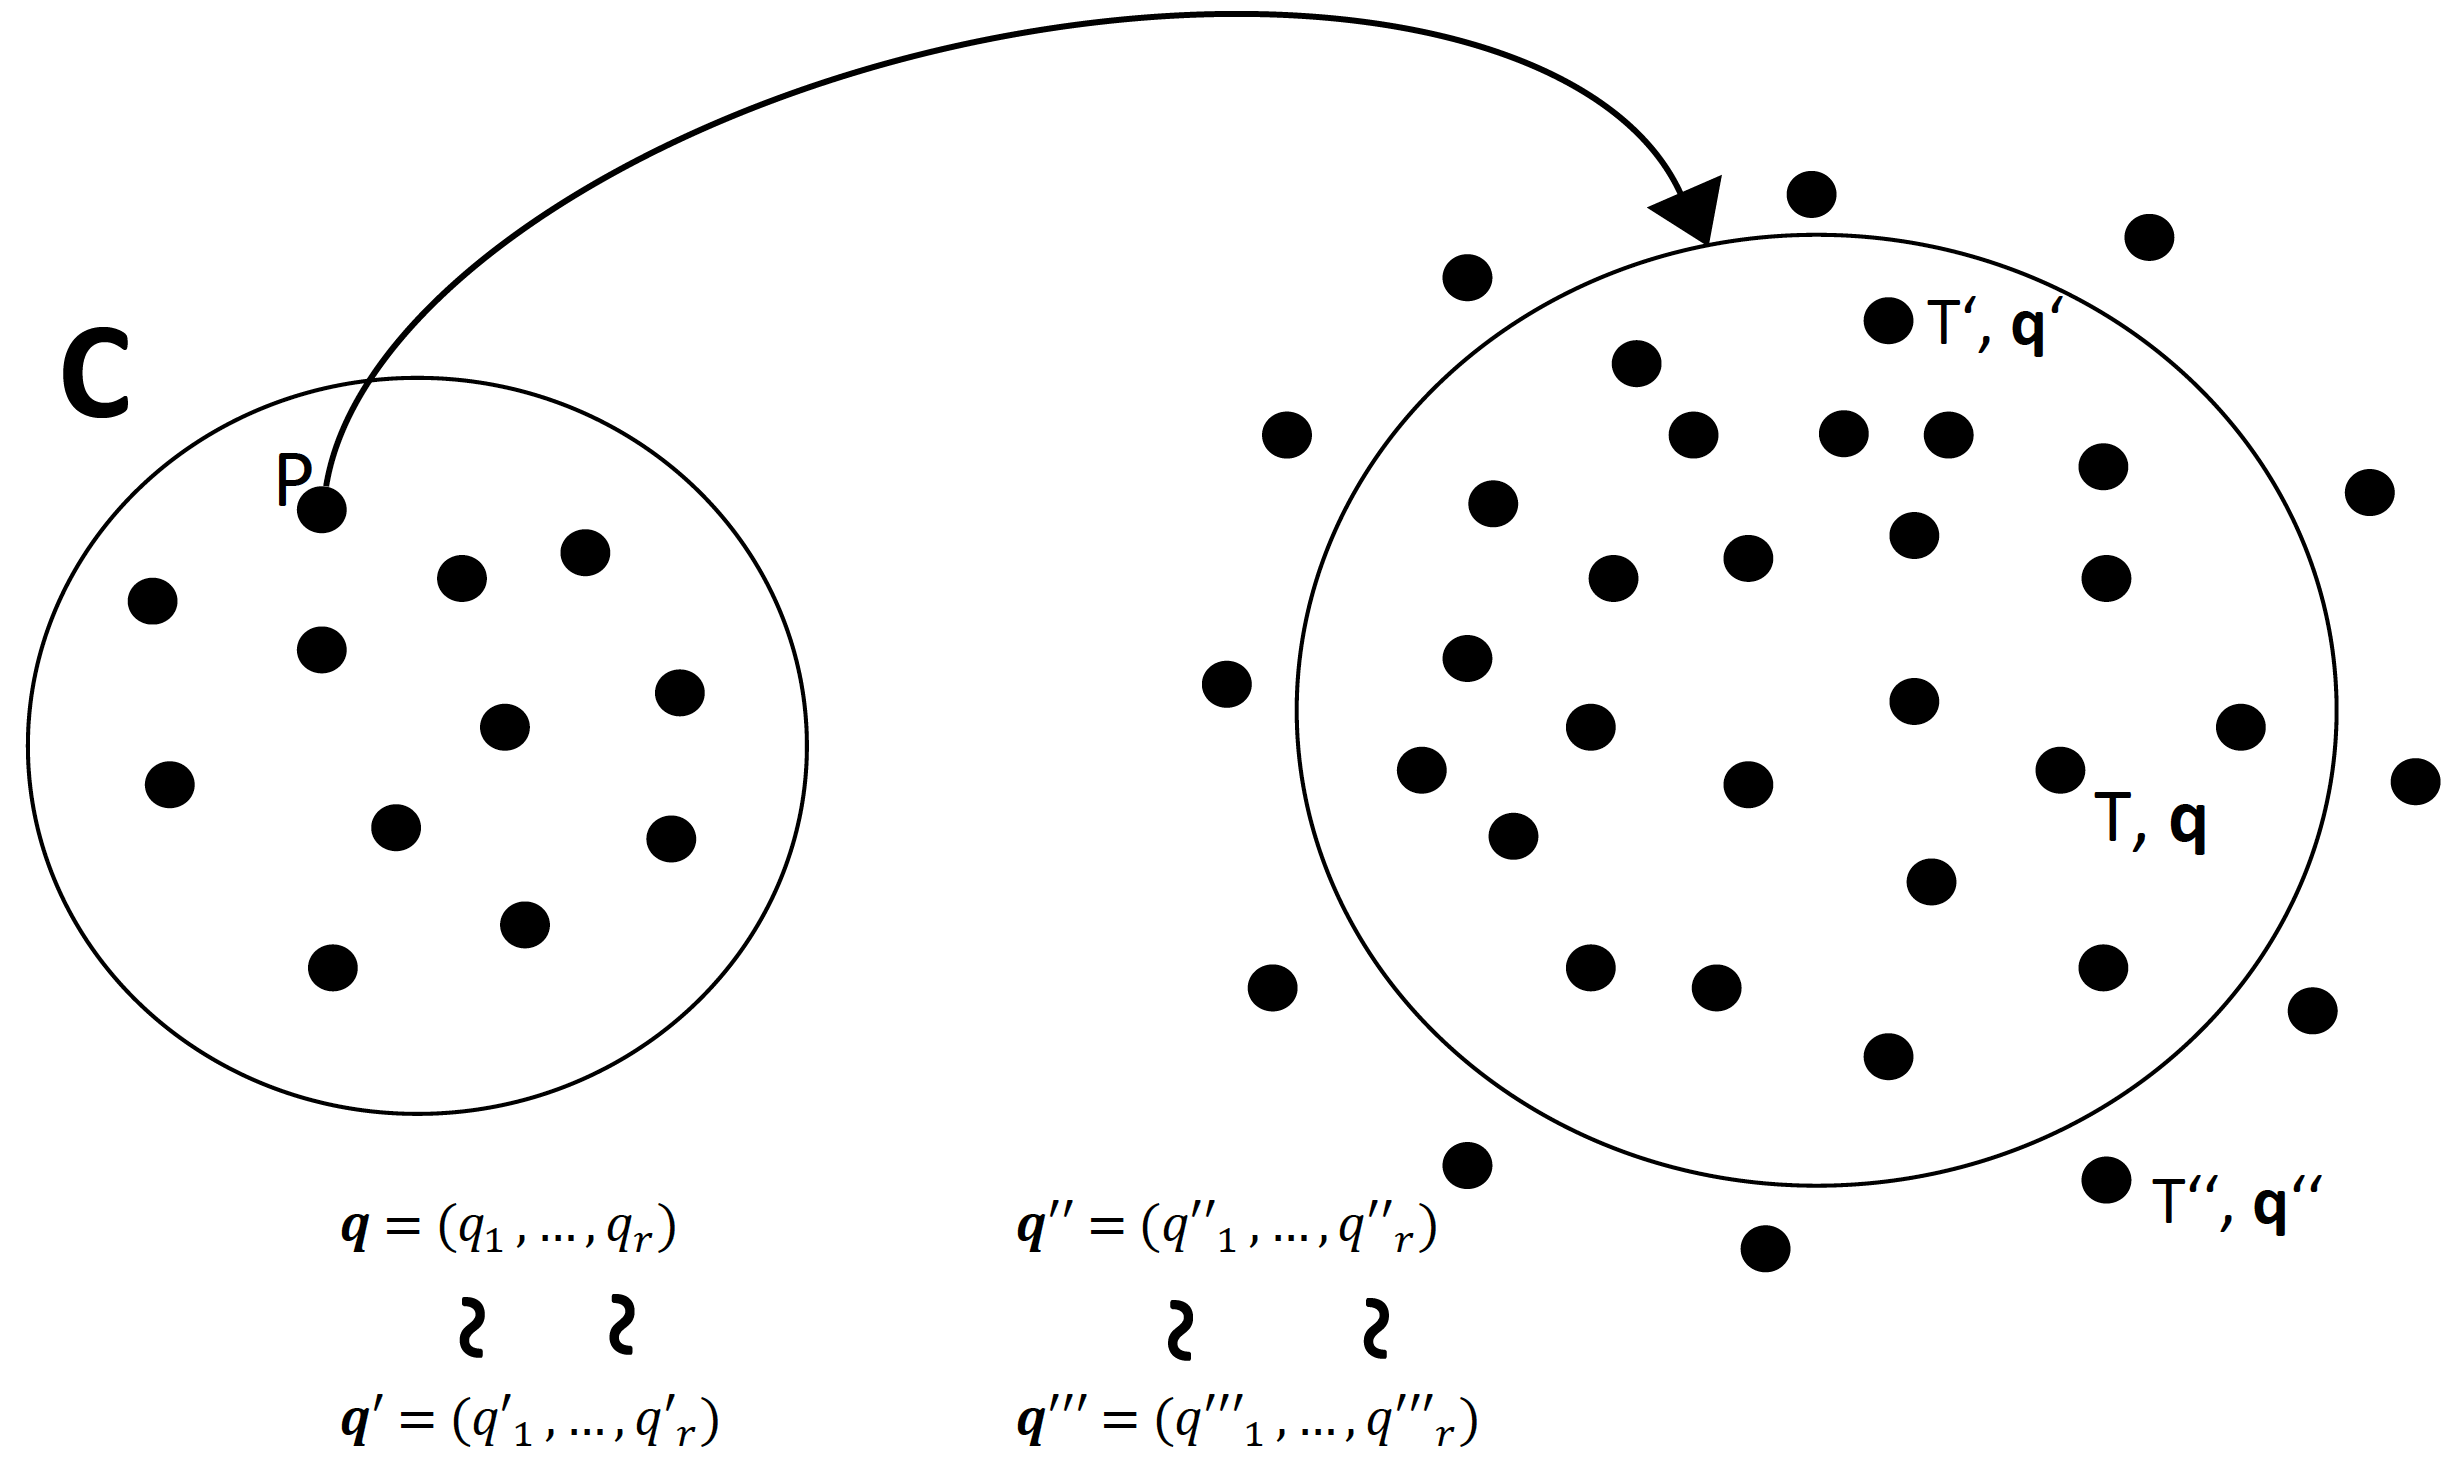
\includegraphics[width=0.9\textwidth]{bisimulation-invariant_4.png}}
  \only<6>{\hspace{-0.6cm}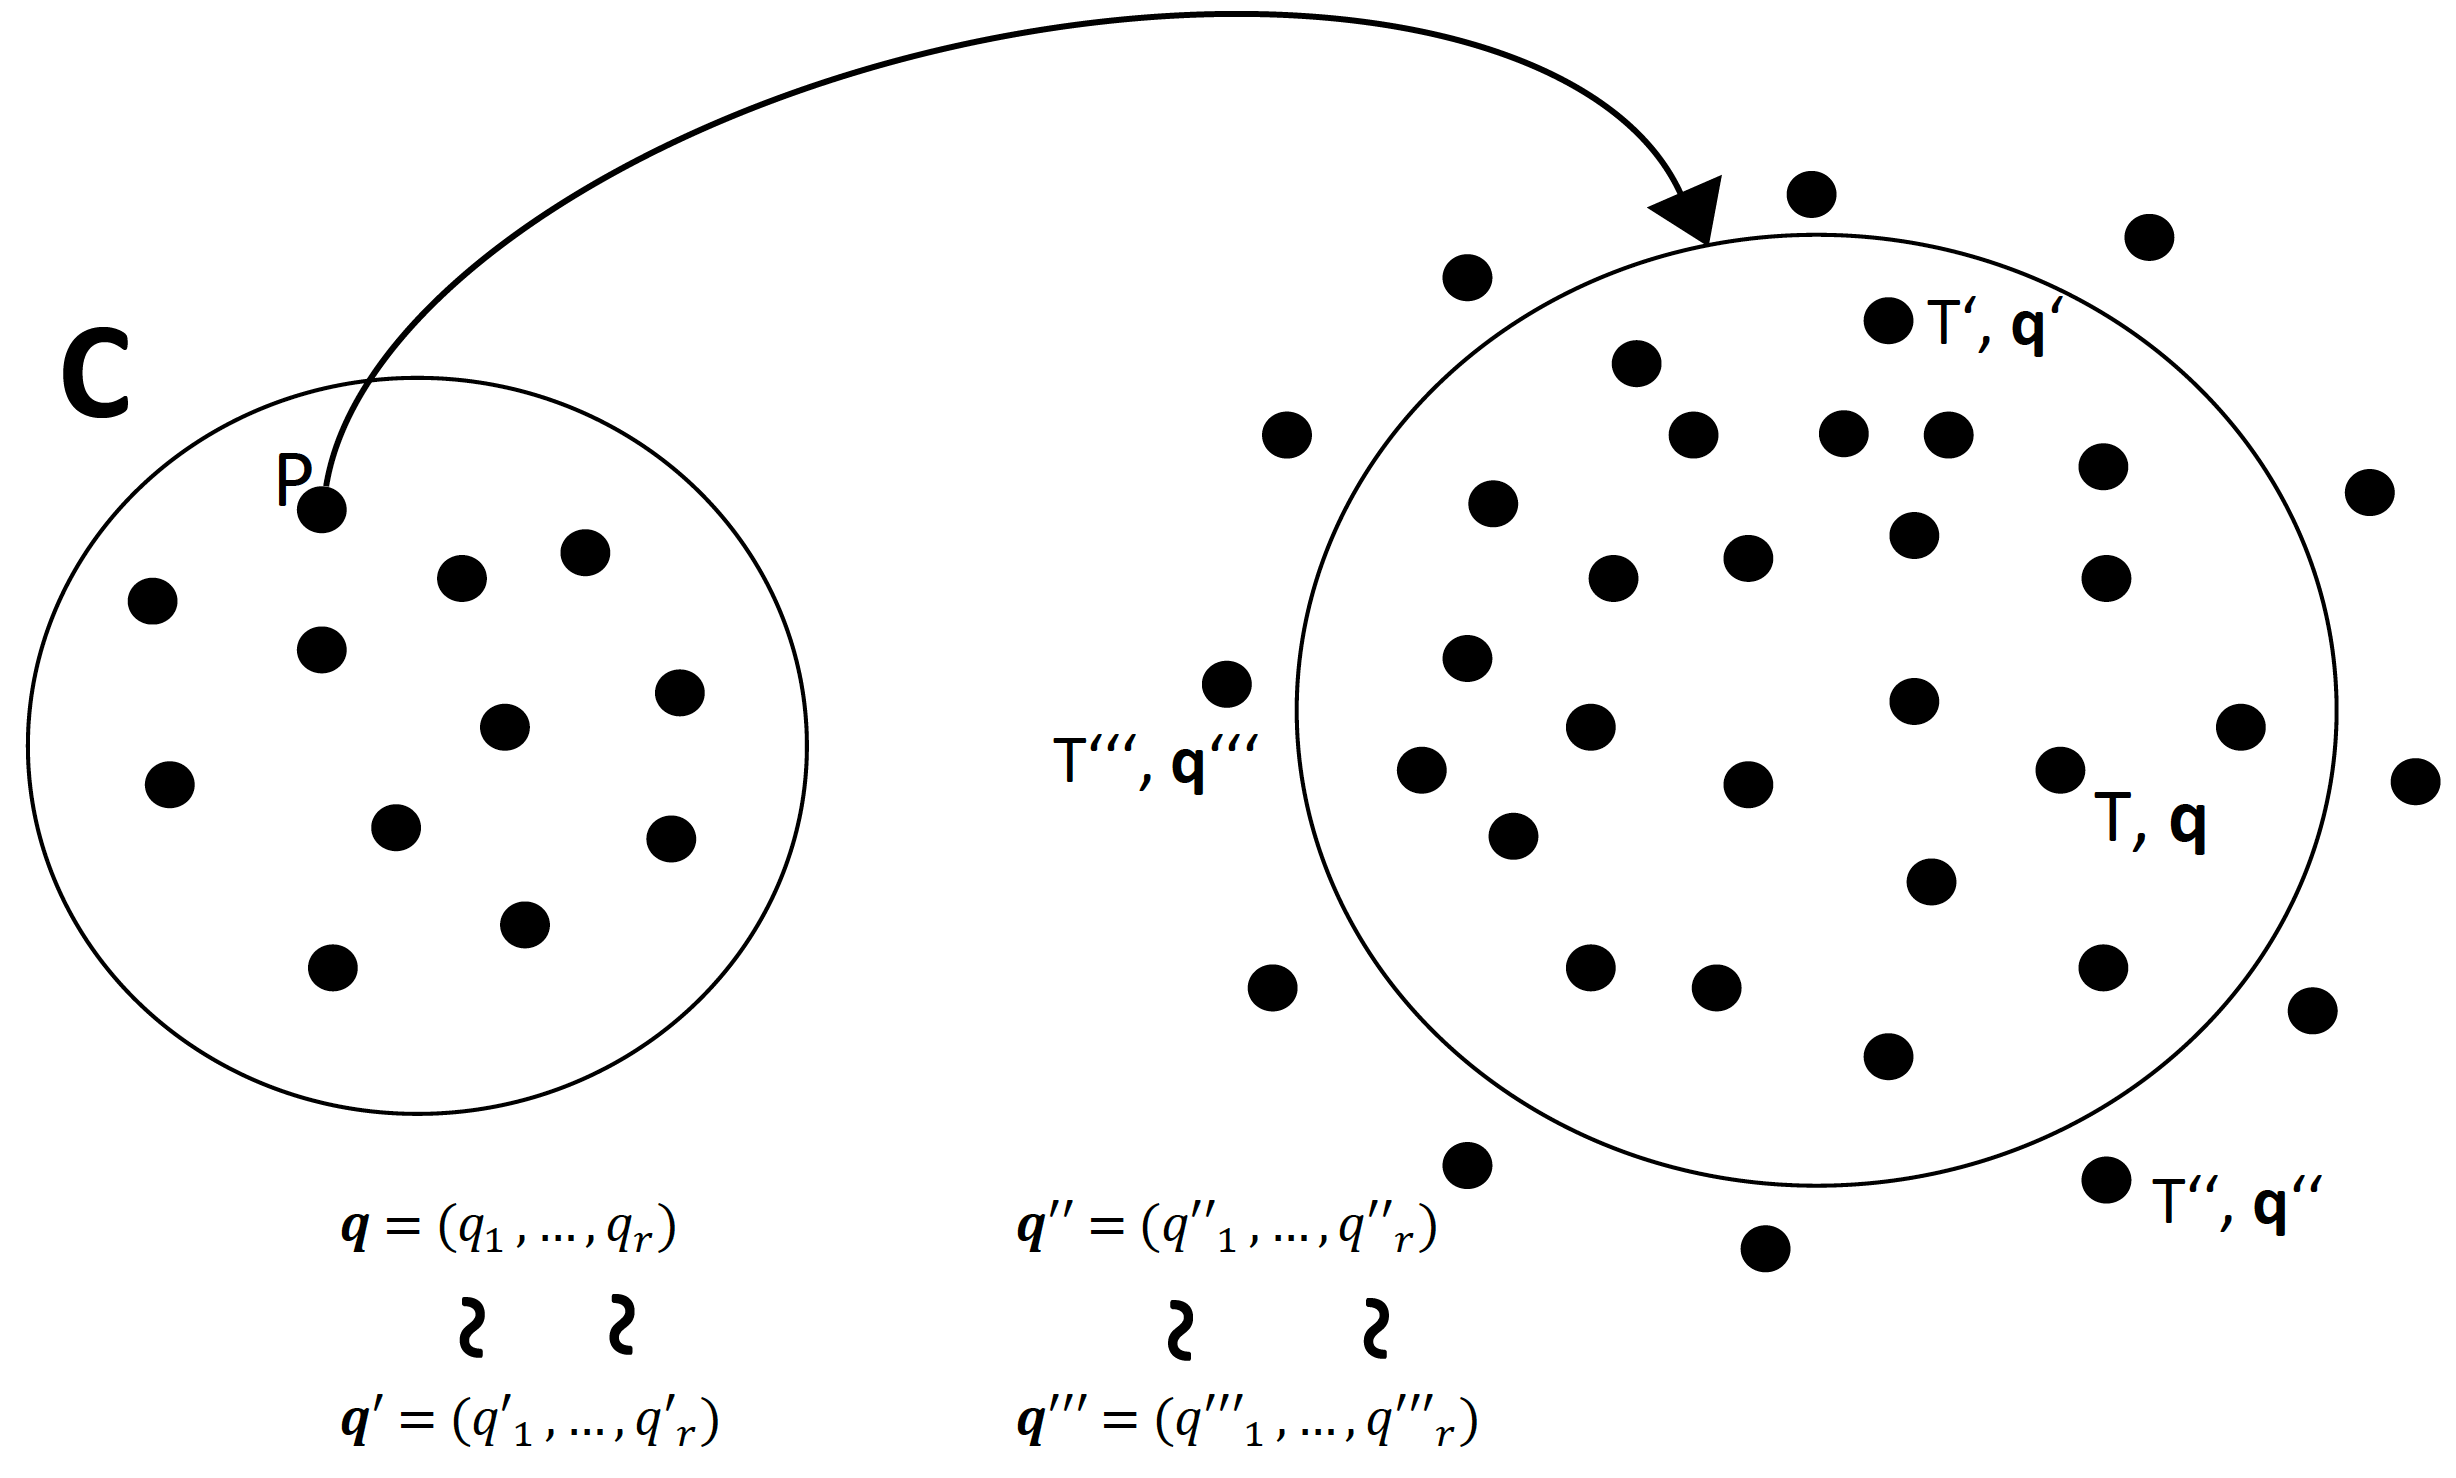
\includegraphics[width=0.9\textwidth]{bisimulation-invariant.png}}}
\end{figure}

\end{frame}
\begin{frame}

Logic captures Complexity Class 

\begin{figure}[ht]
	\centering{
  \only<1>{\hspace{-0.1cm}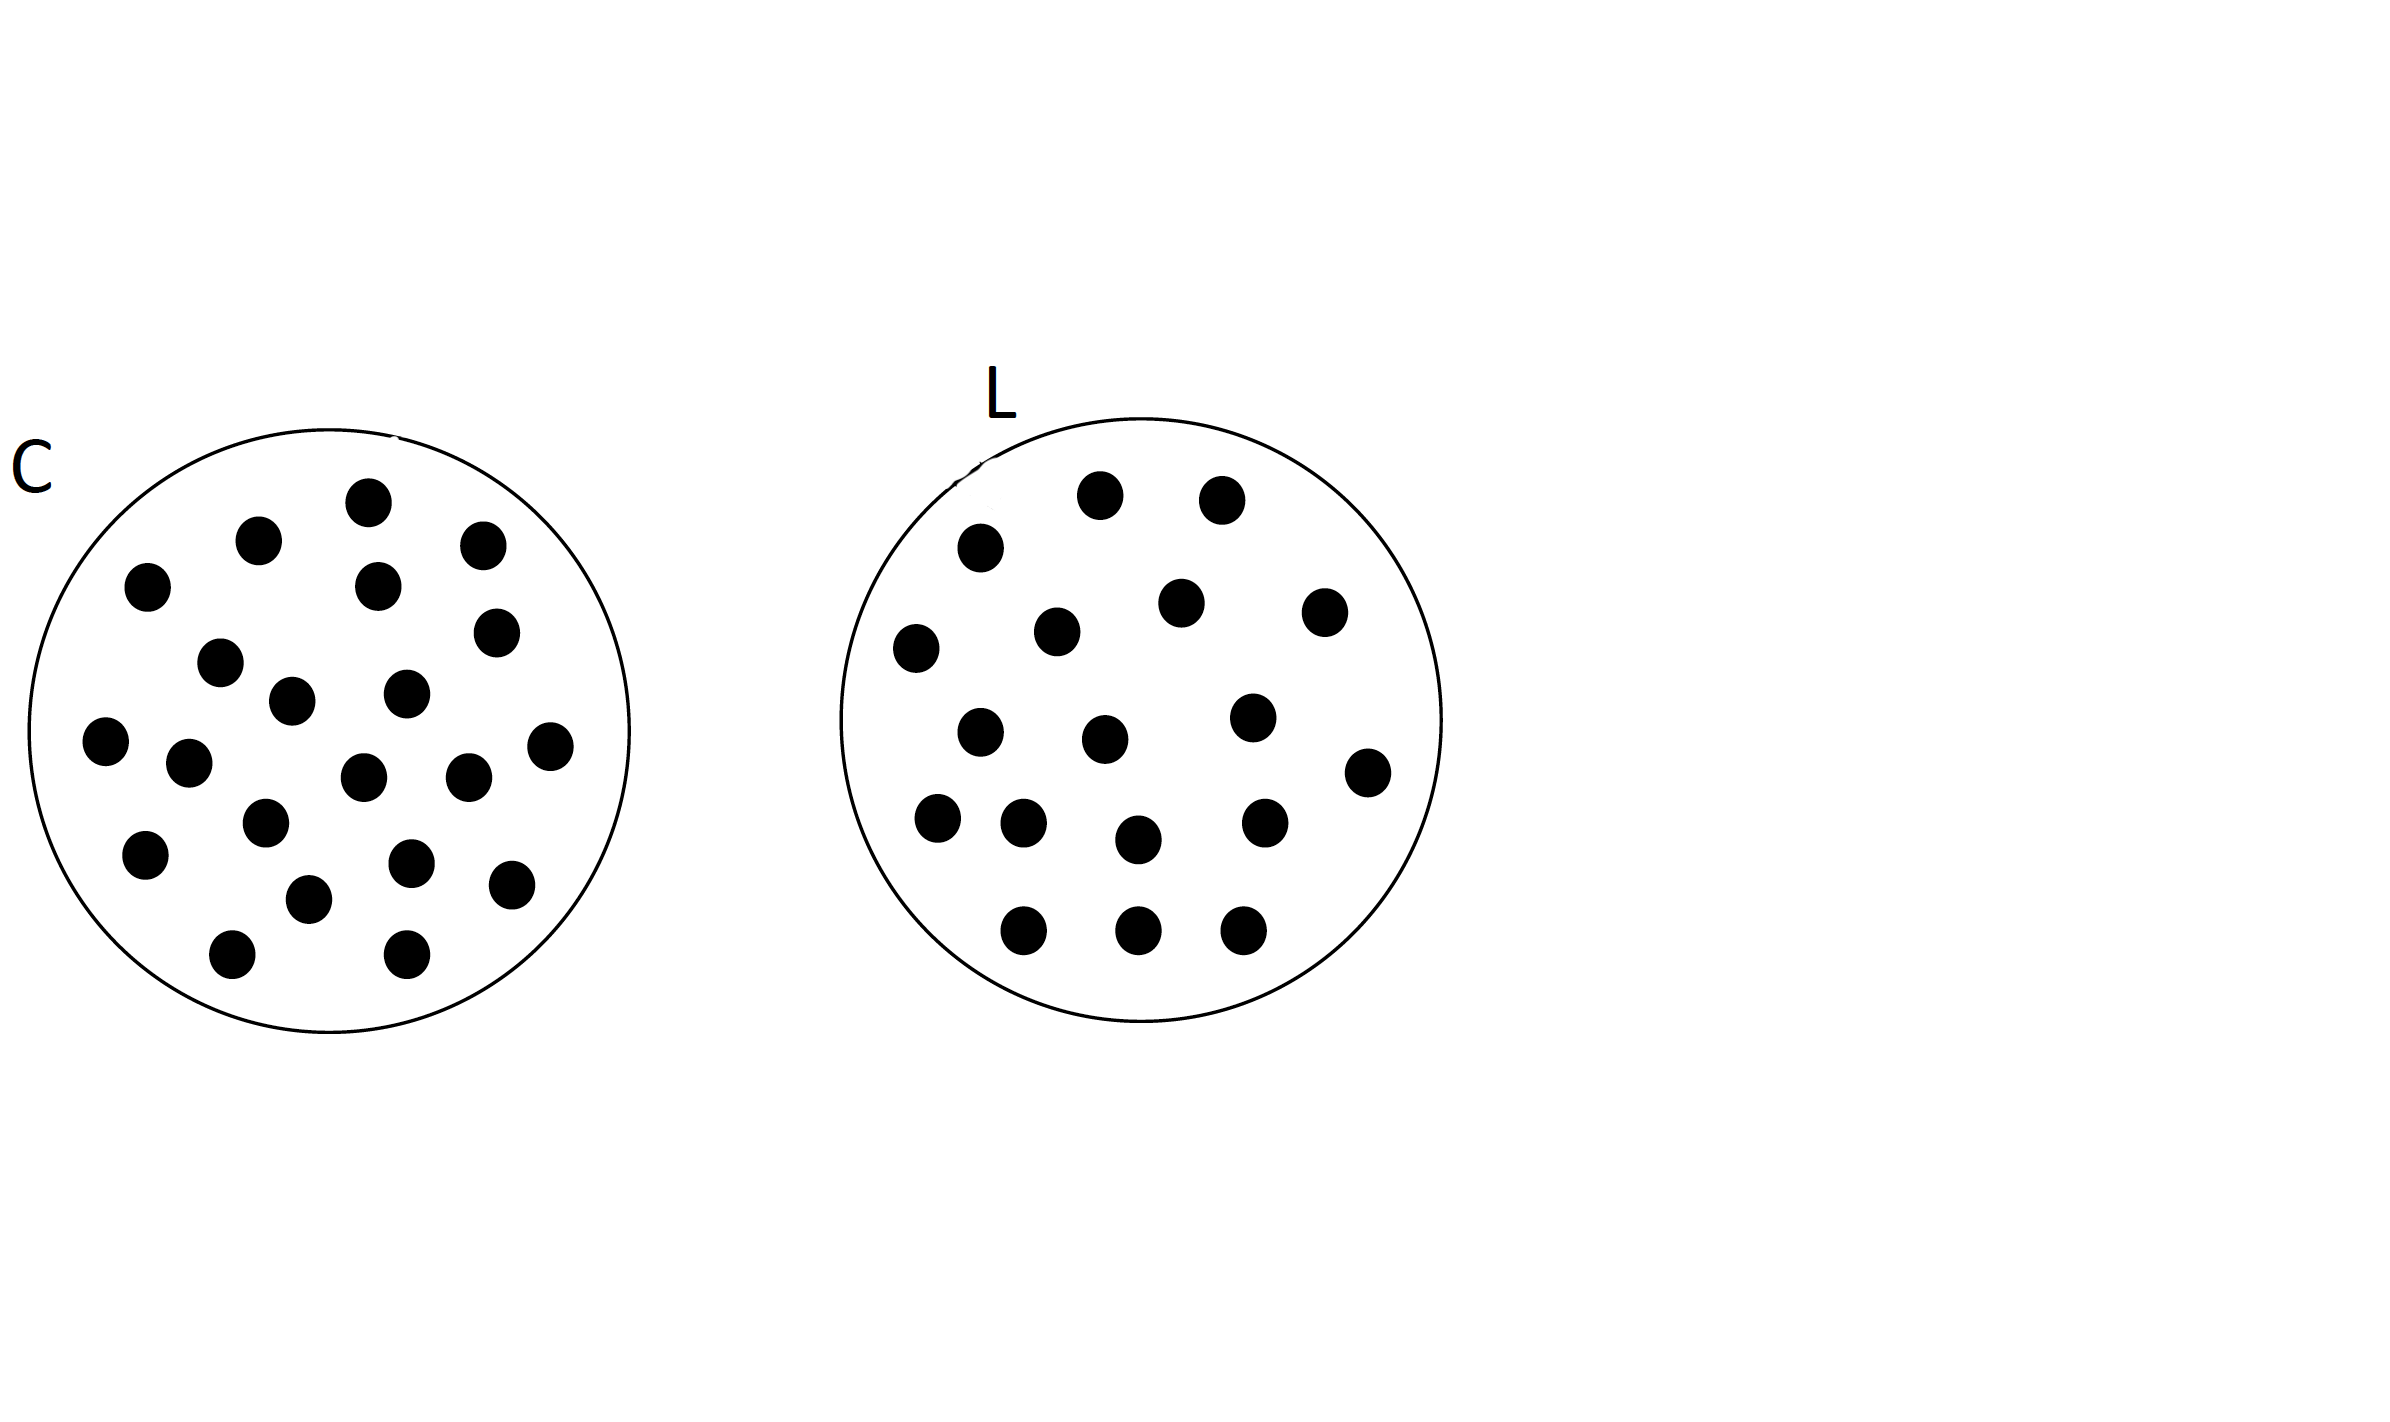
\includegraphics[width=0.9\textwidth]{logic-capture-class_0.png}}
  \only<2>{\hspace{-0.1cm}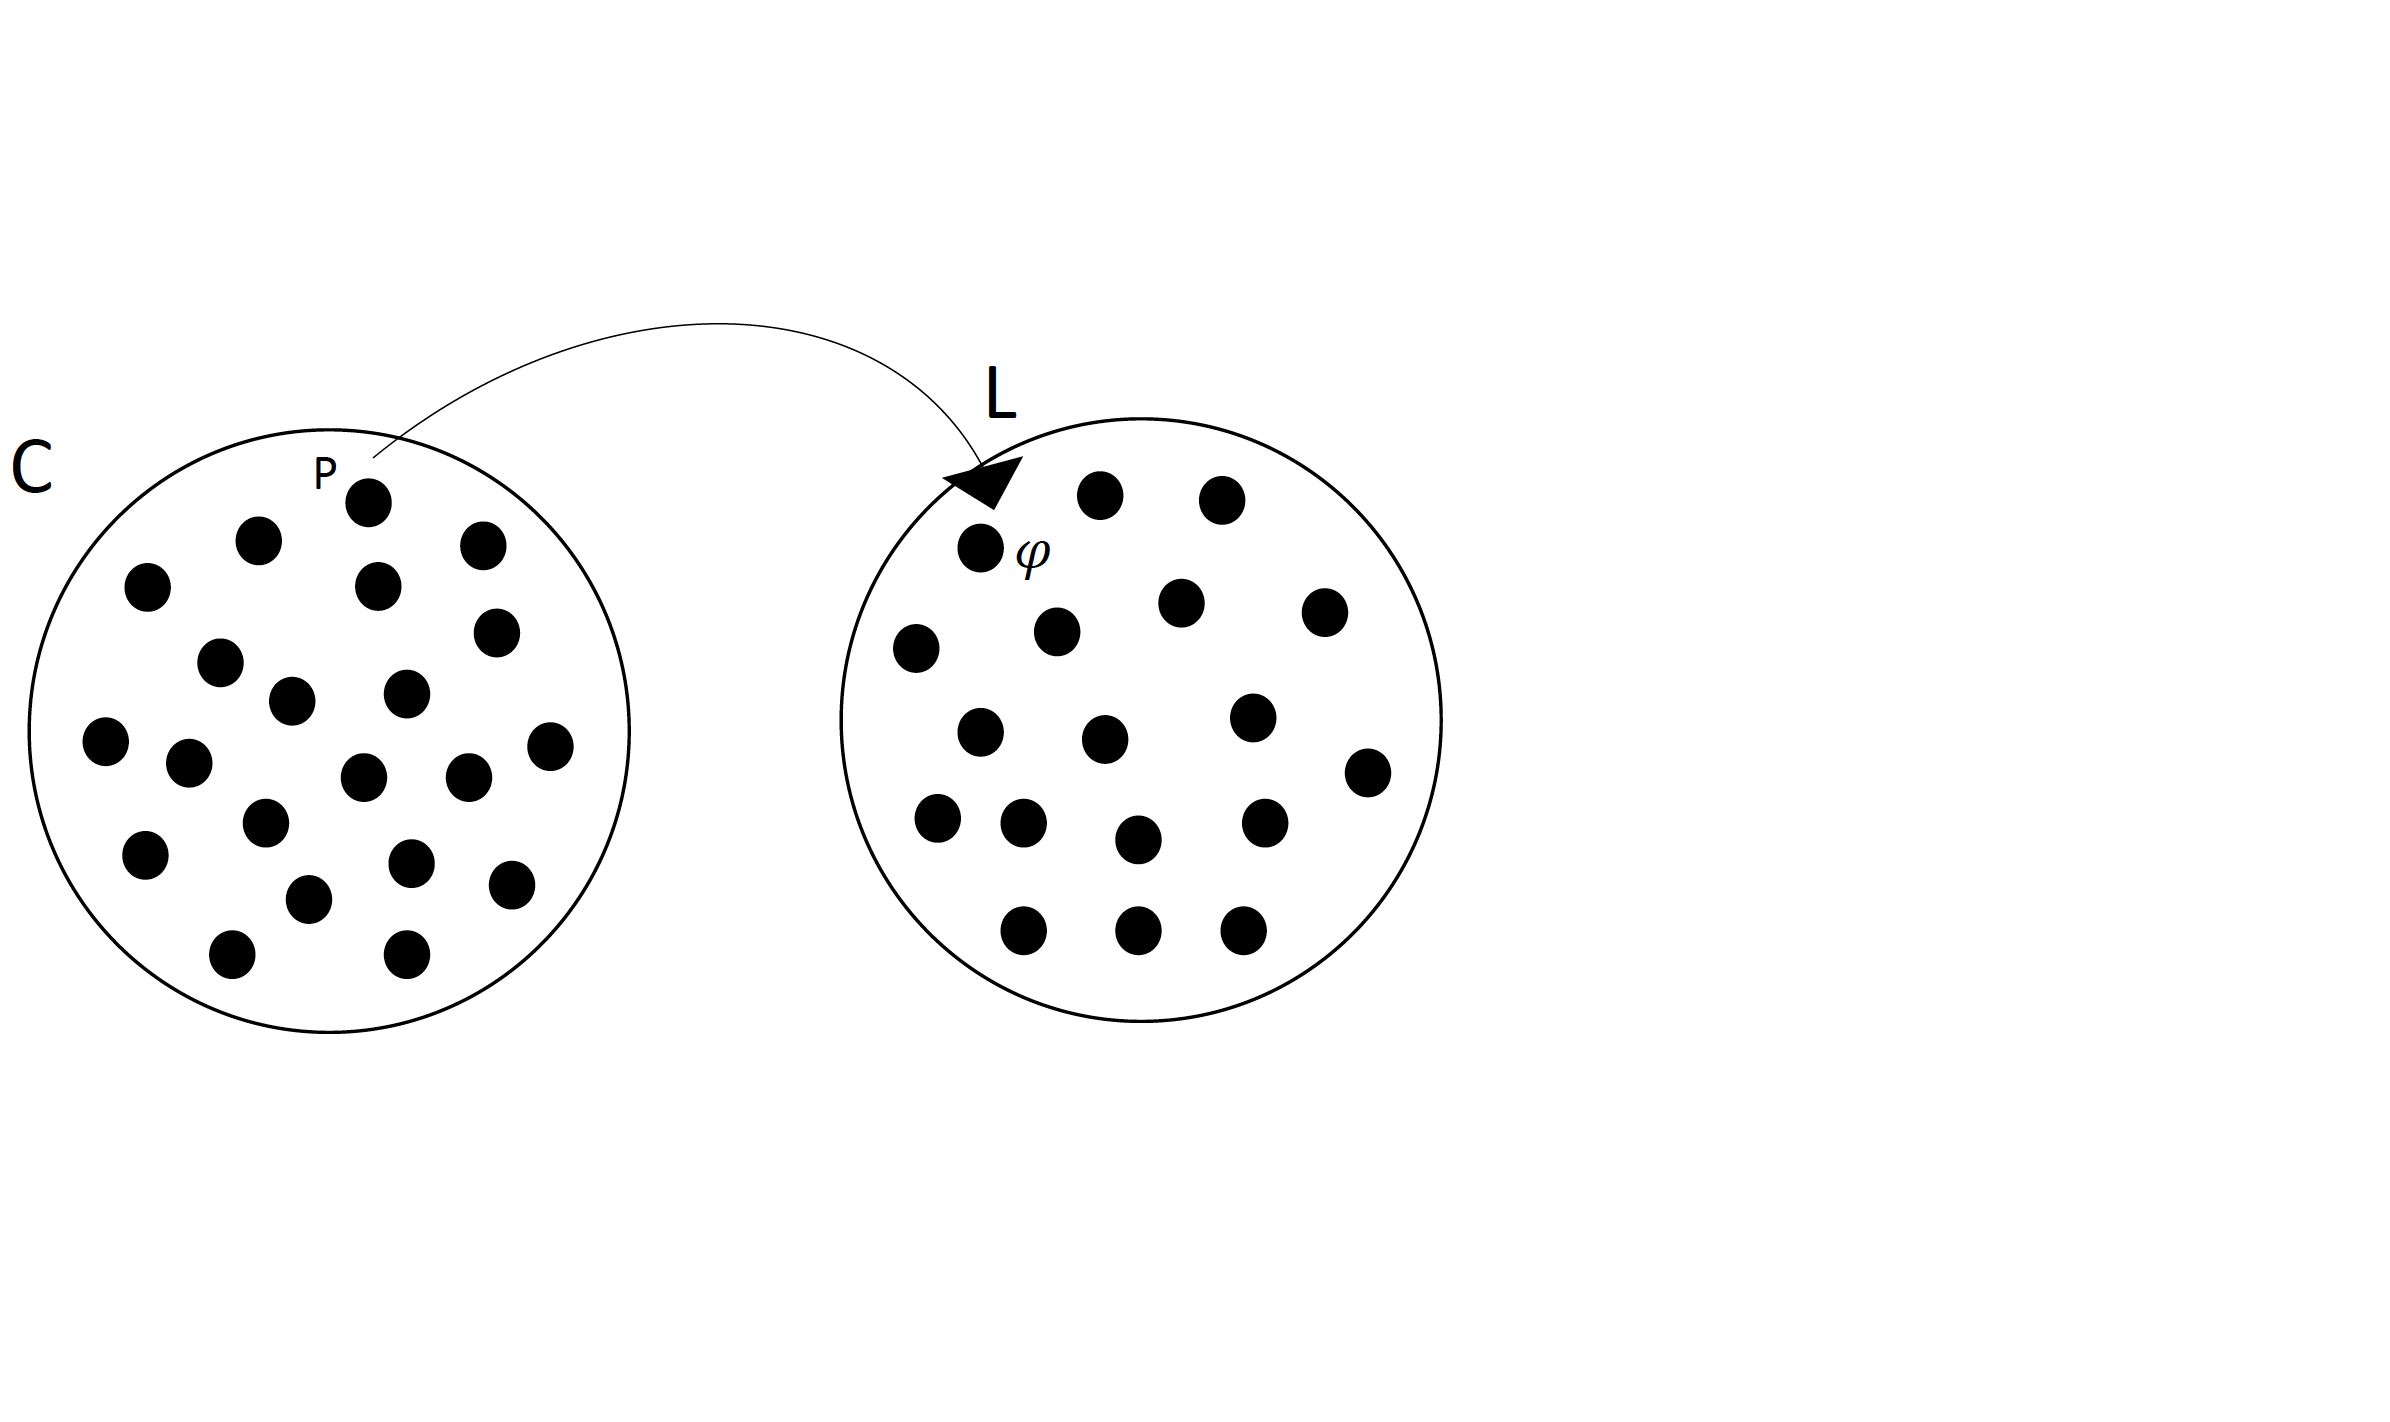
\includegraphics[width=0.9\textwidth]{logic-capture-class_1.png}}
  \only<3>{\hspace{-0.2cm}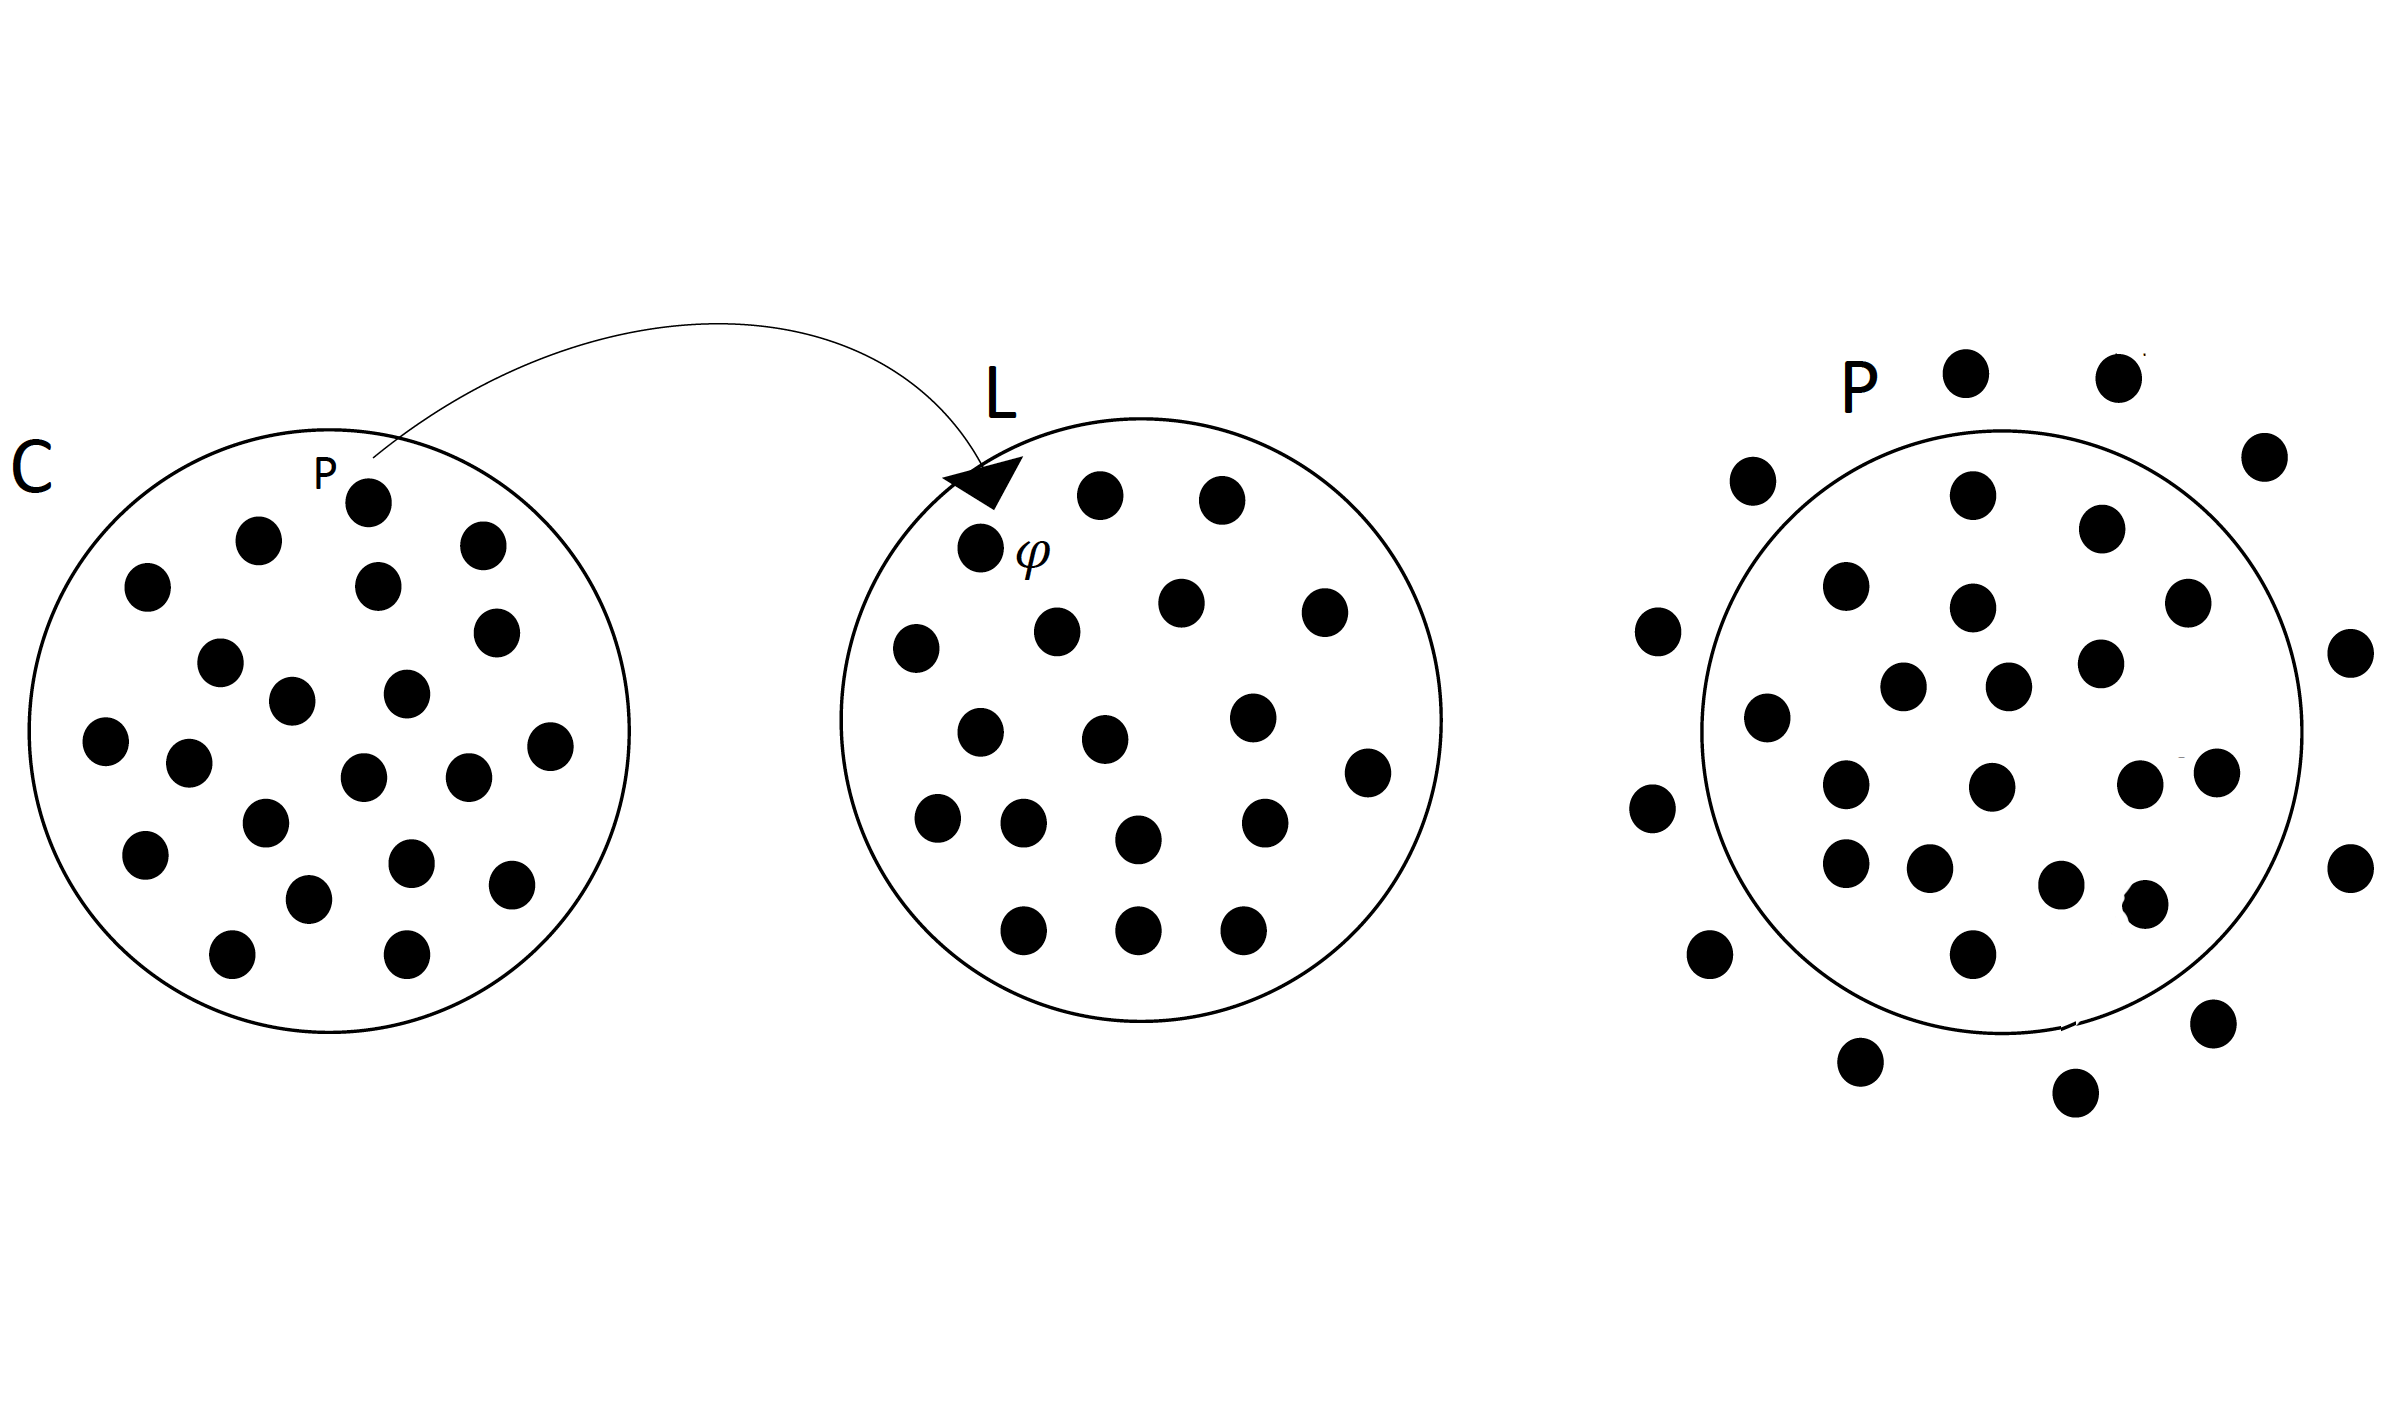
\includegraphics[width=0.9\textwidth]{logic-capture-class_2.png}}
  \only<4>{\hspace{-0.3cm}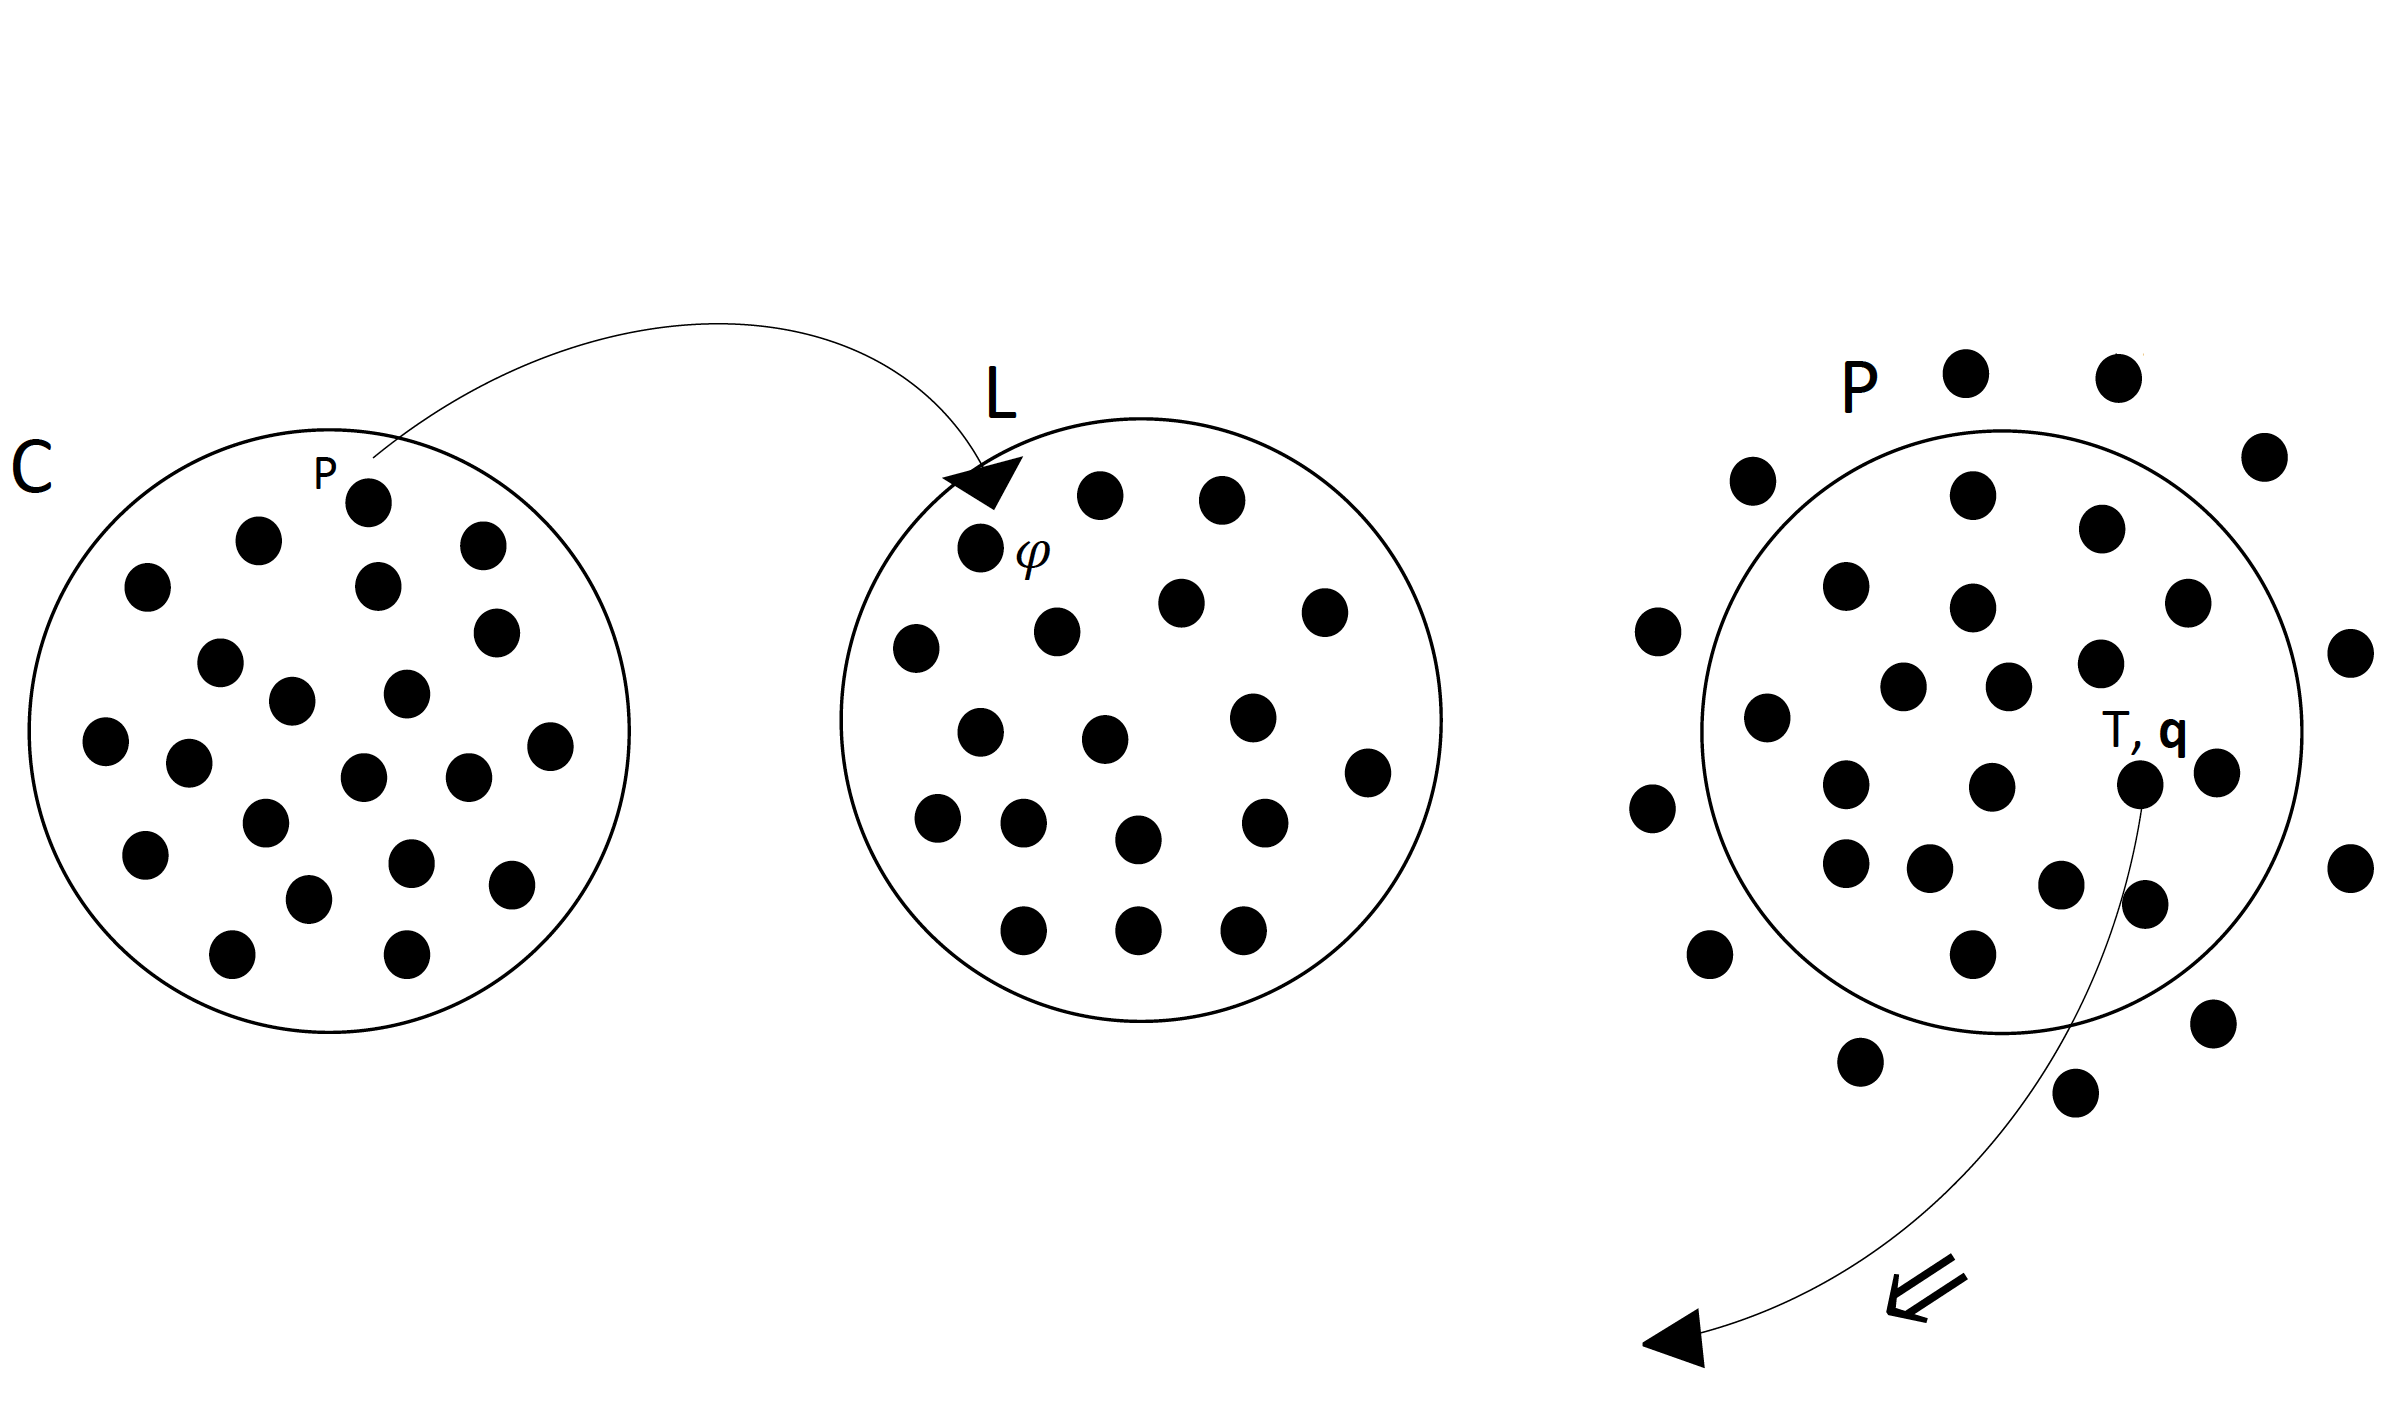
\includegraphics[width=0.9\textwidth]{logic-capture-class_3.png}}
  \only<5>{\hspace{-0.4cm}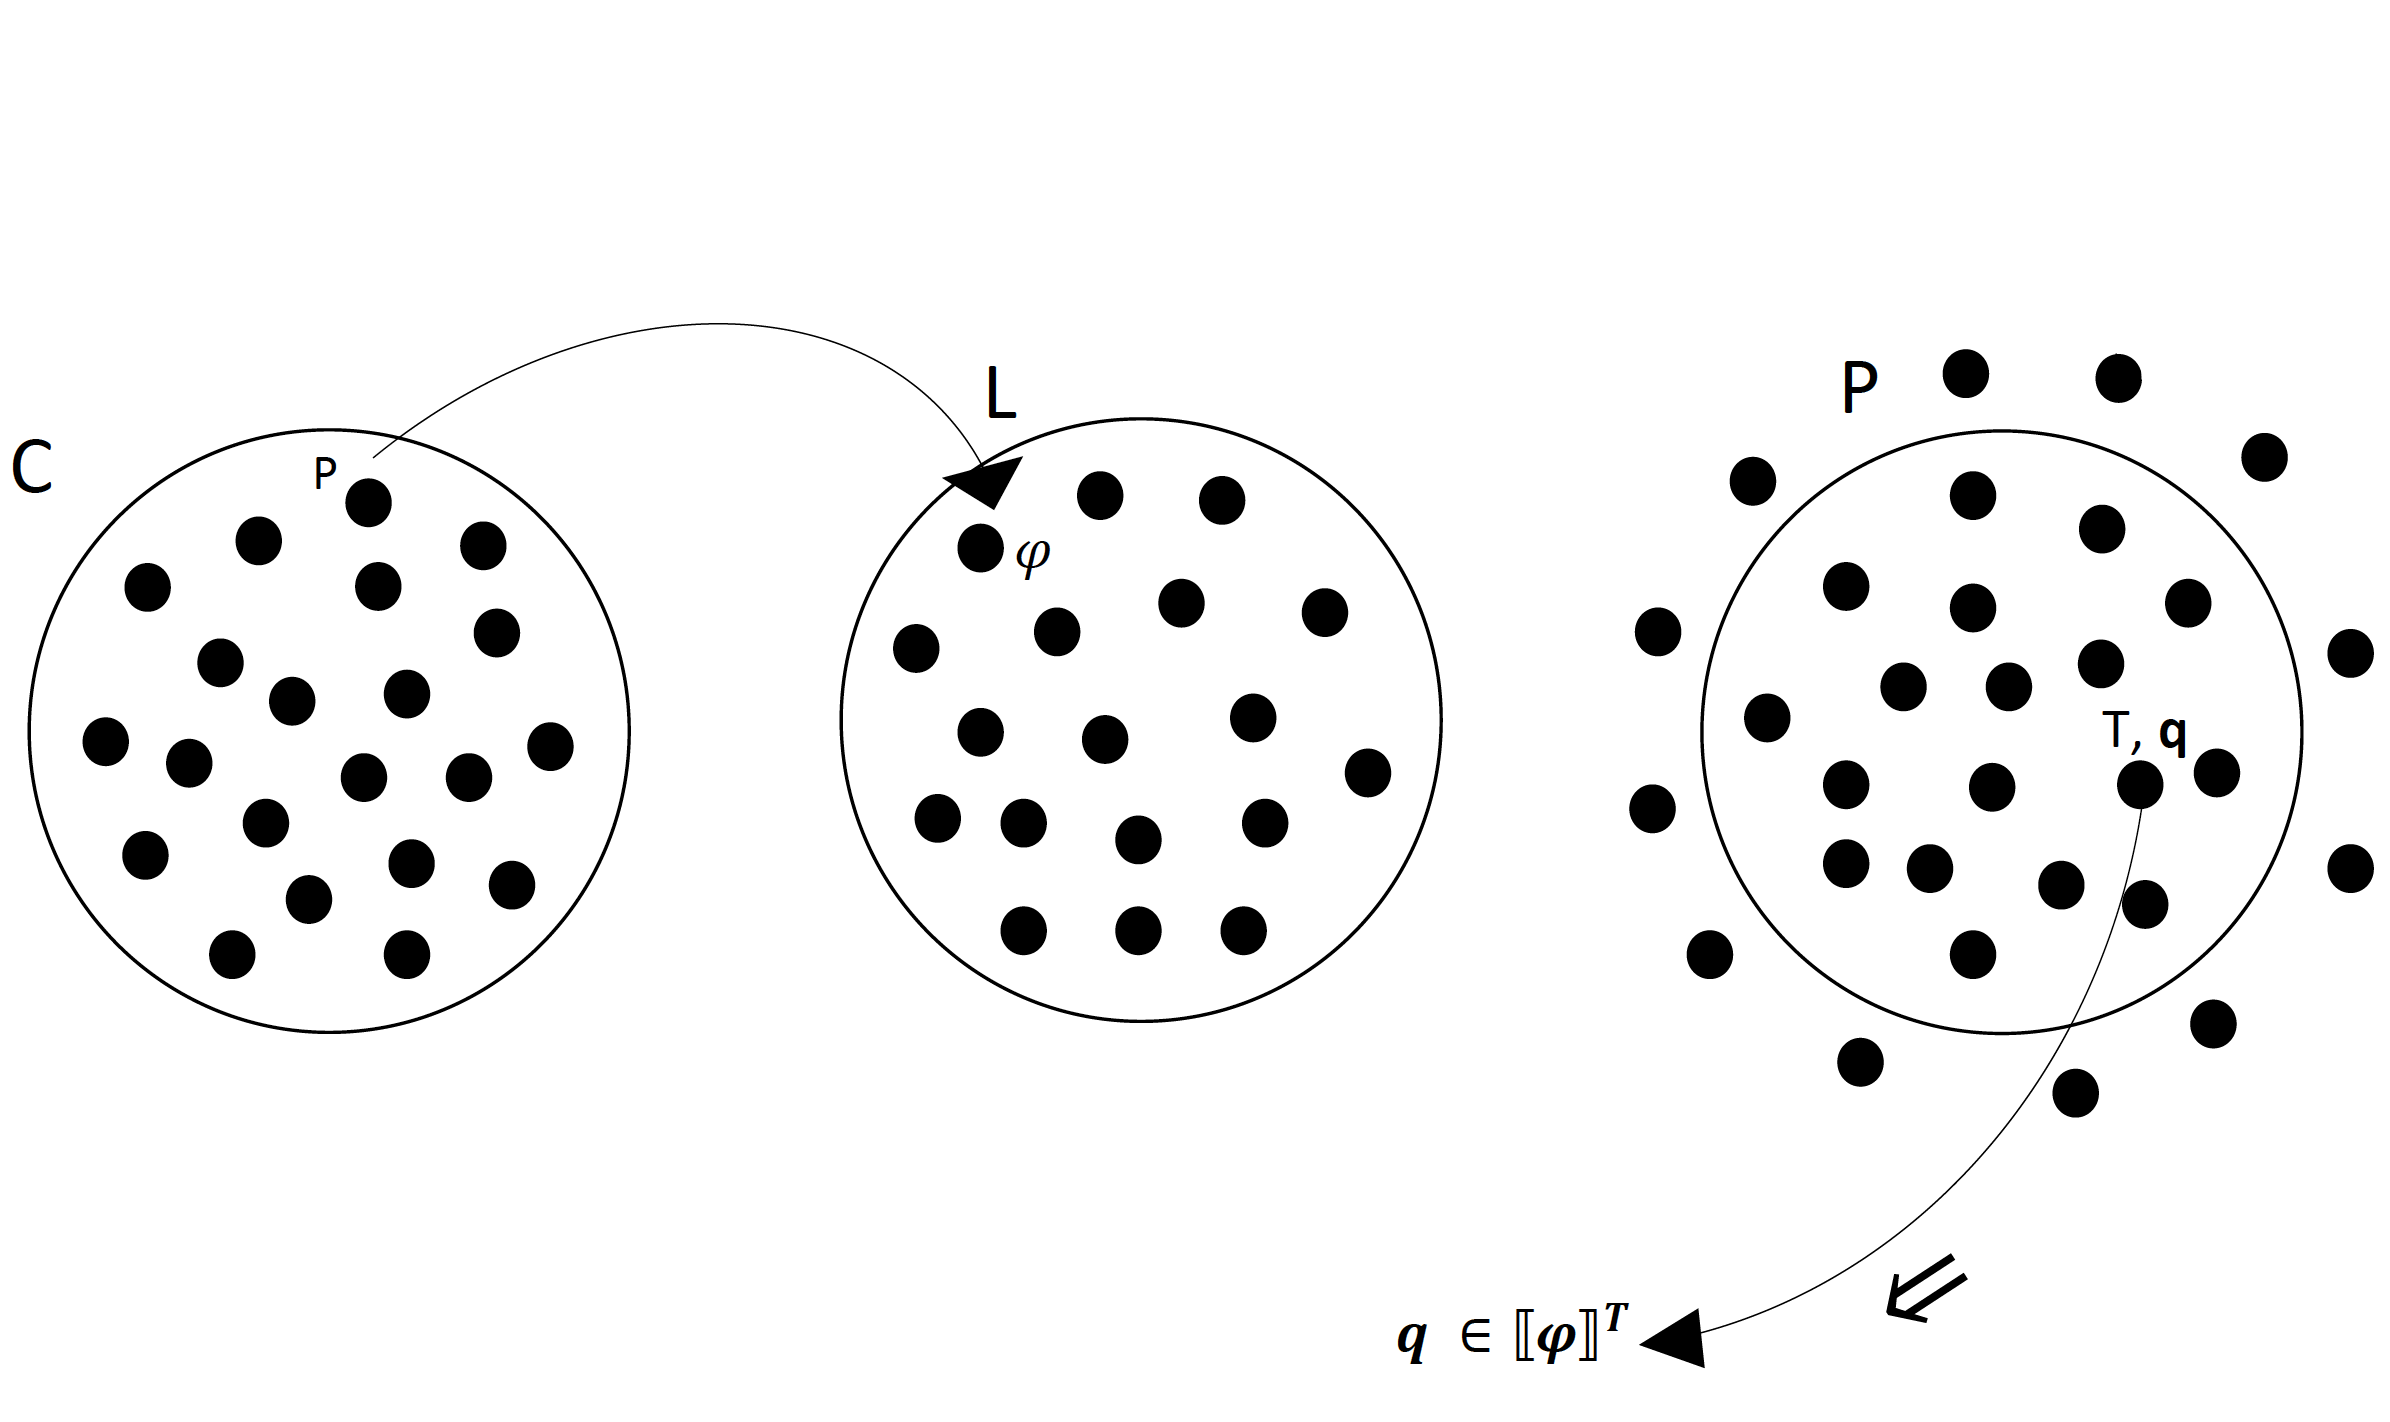
\includegraphics[width=0.9\textwidth]{logic-capture-class_4.png}}
  \only<6>{\hspace{-0.5cm}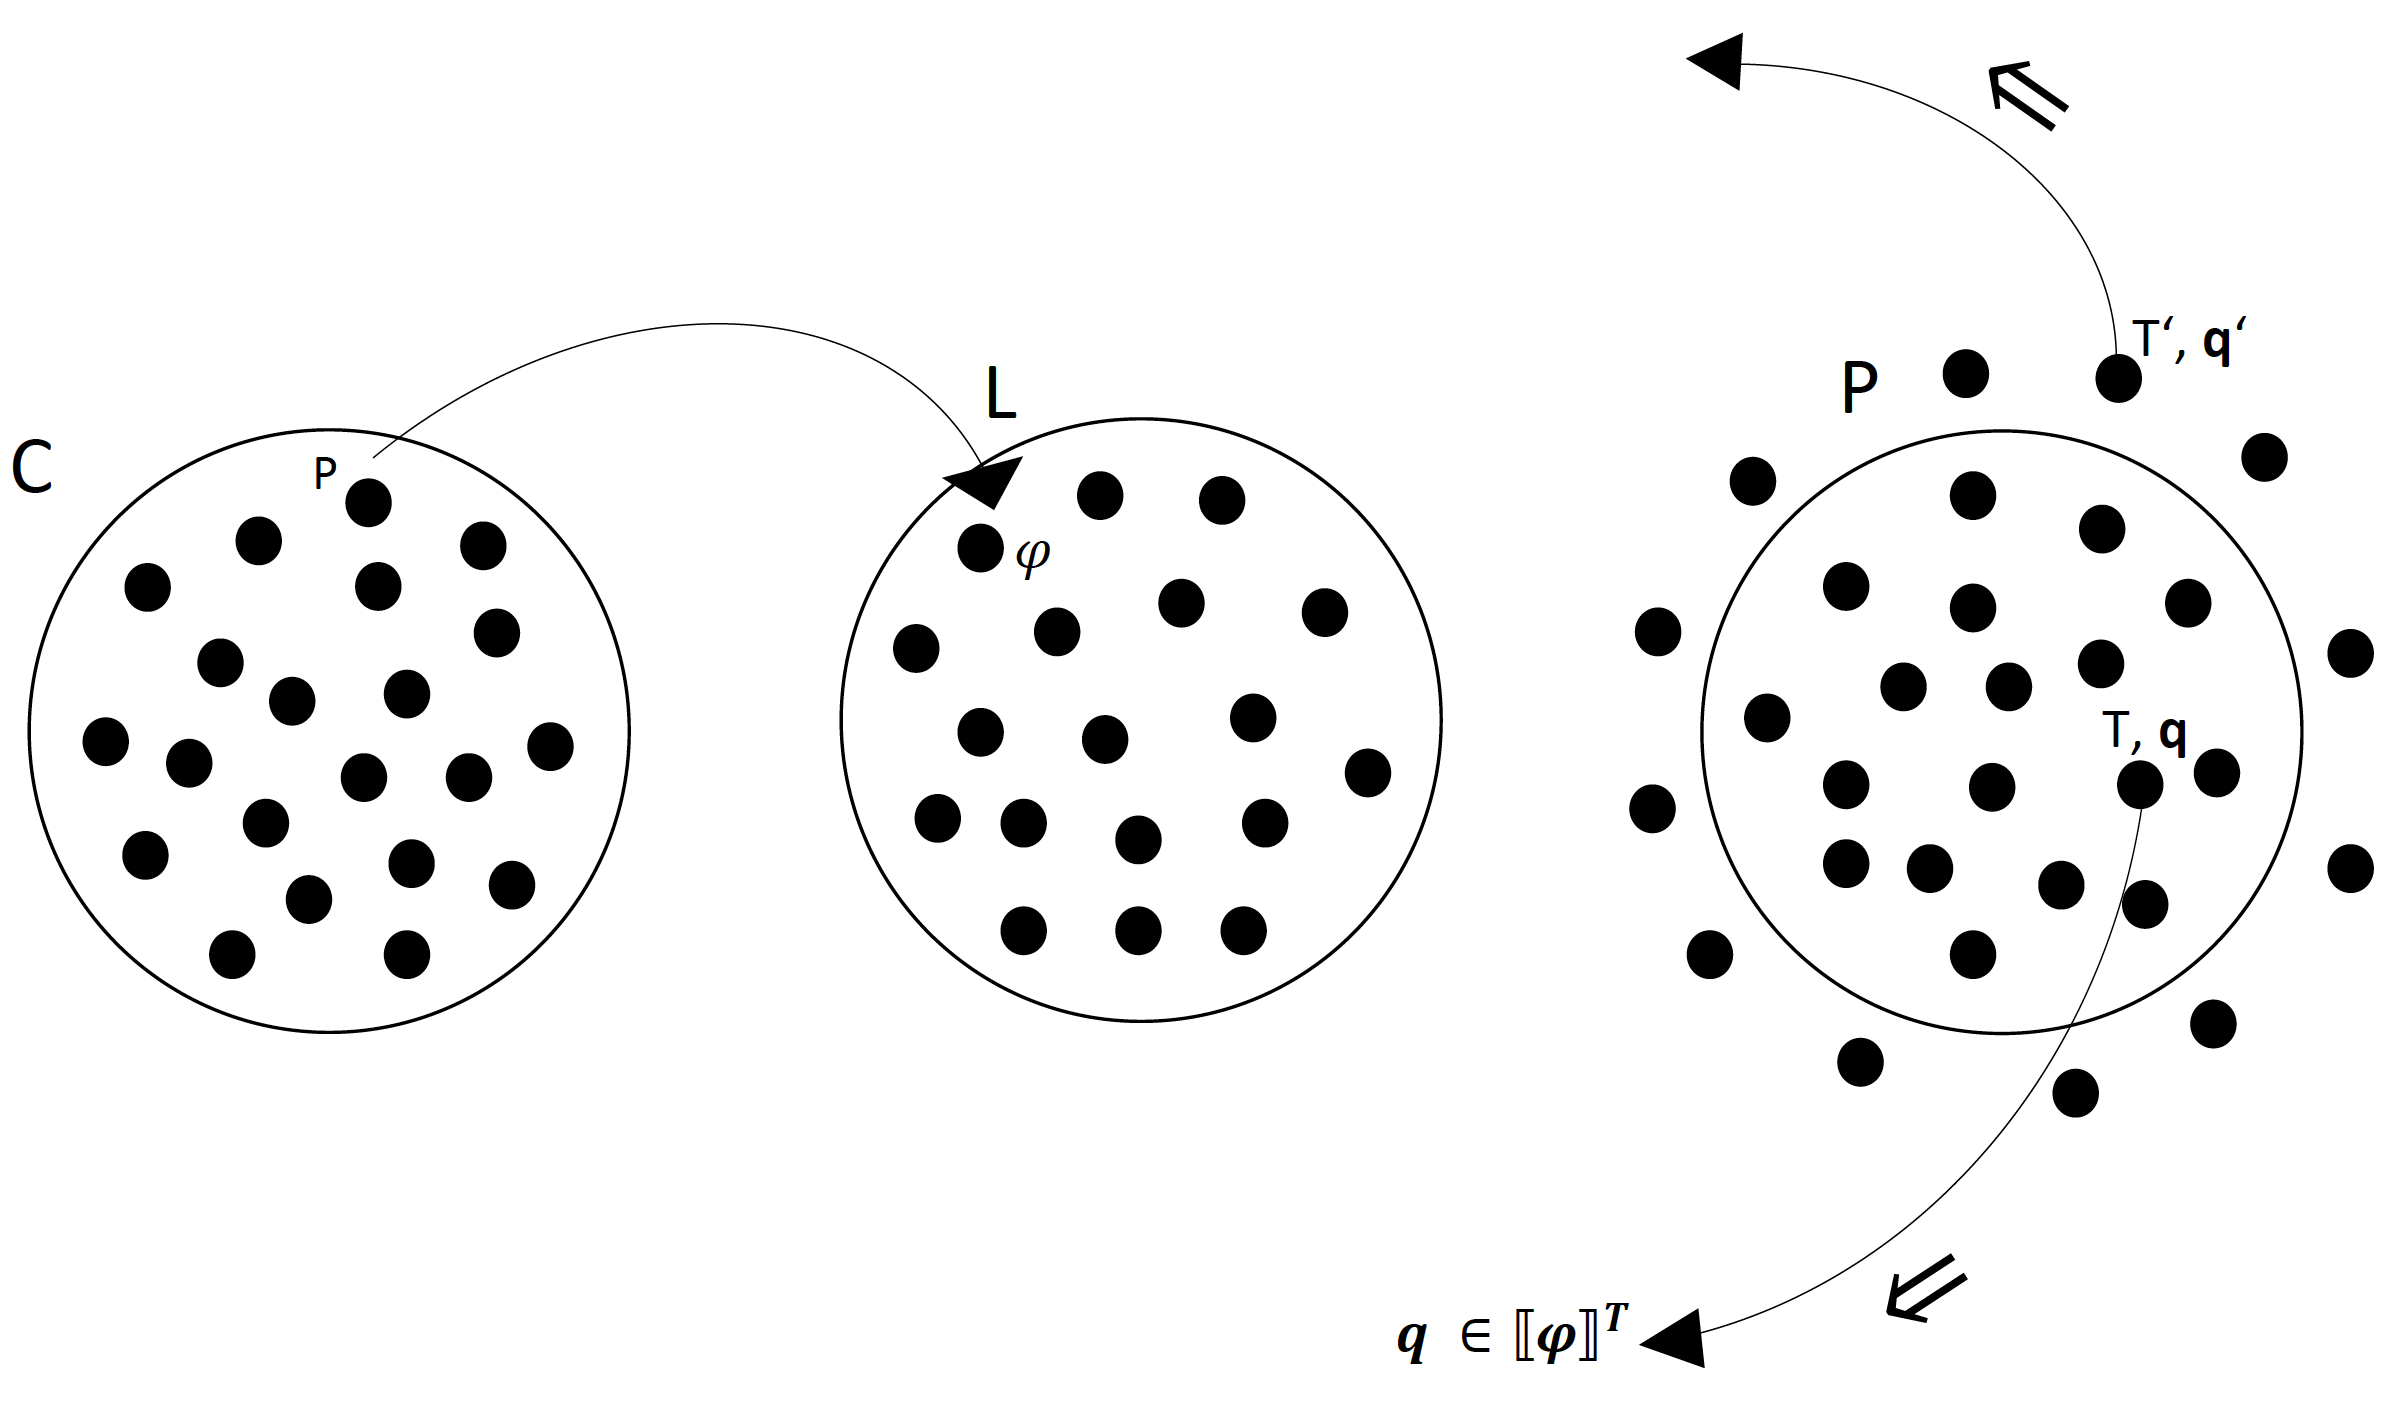
\includegraphics[width=0.9\textwidth]{logic-capture-class_5.png}}
  \only<7>{\hspace{-0.6cm}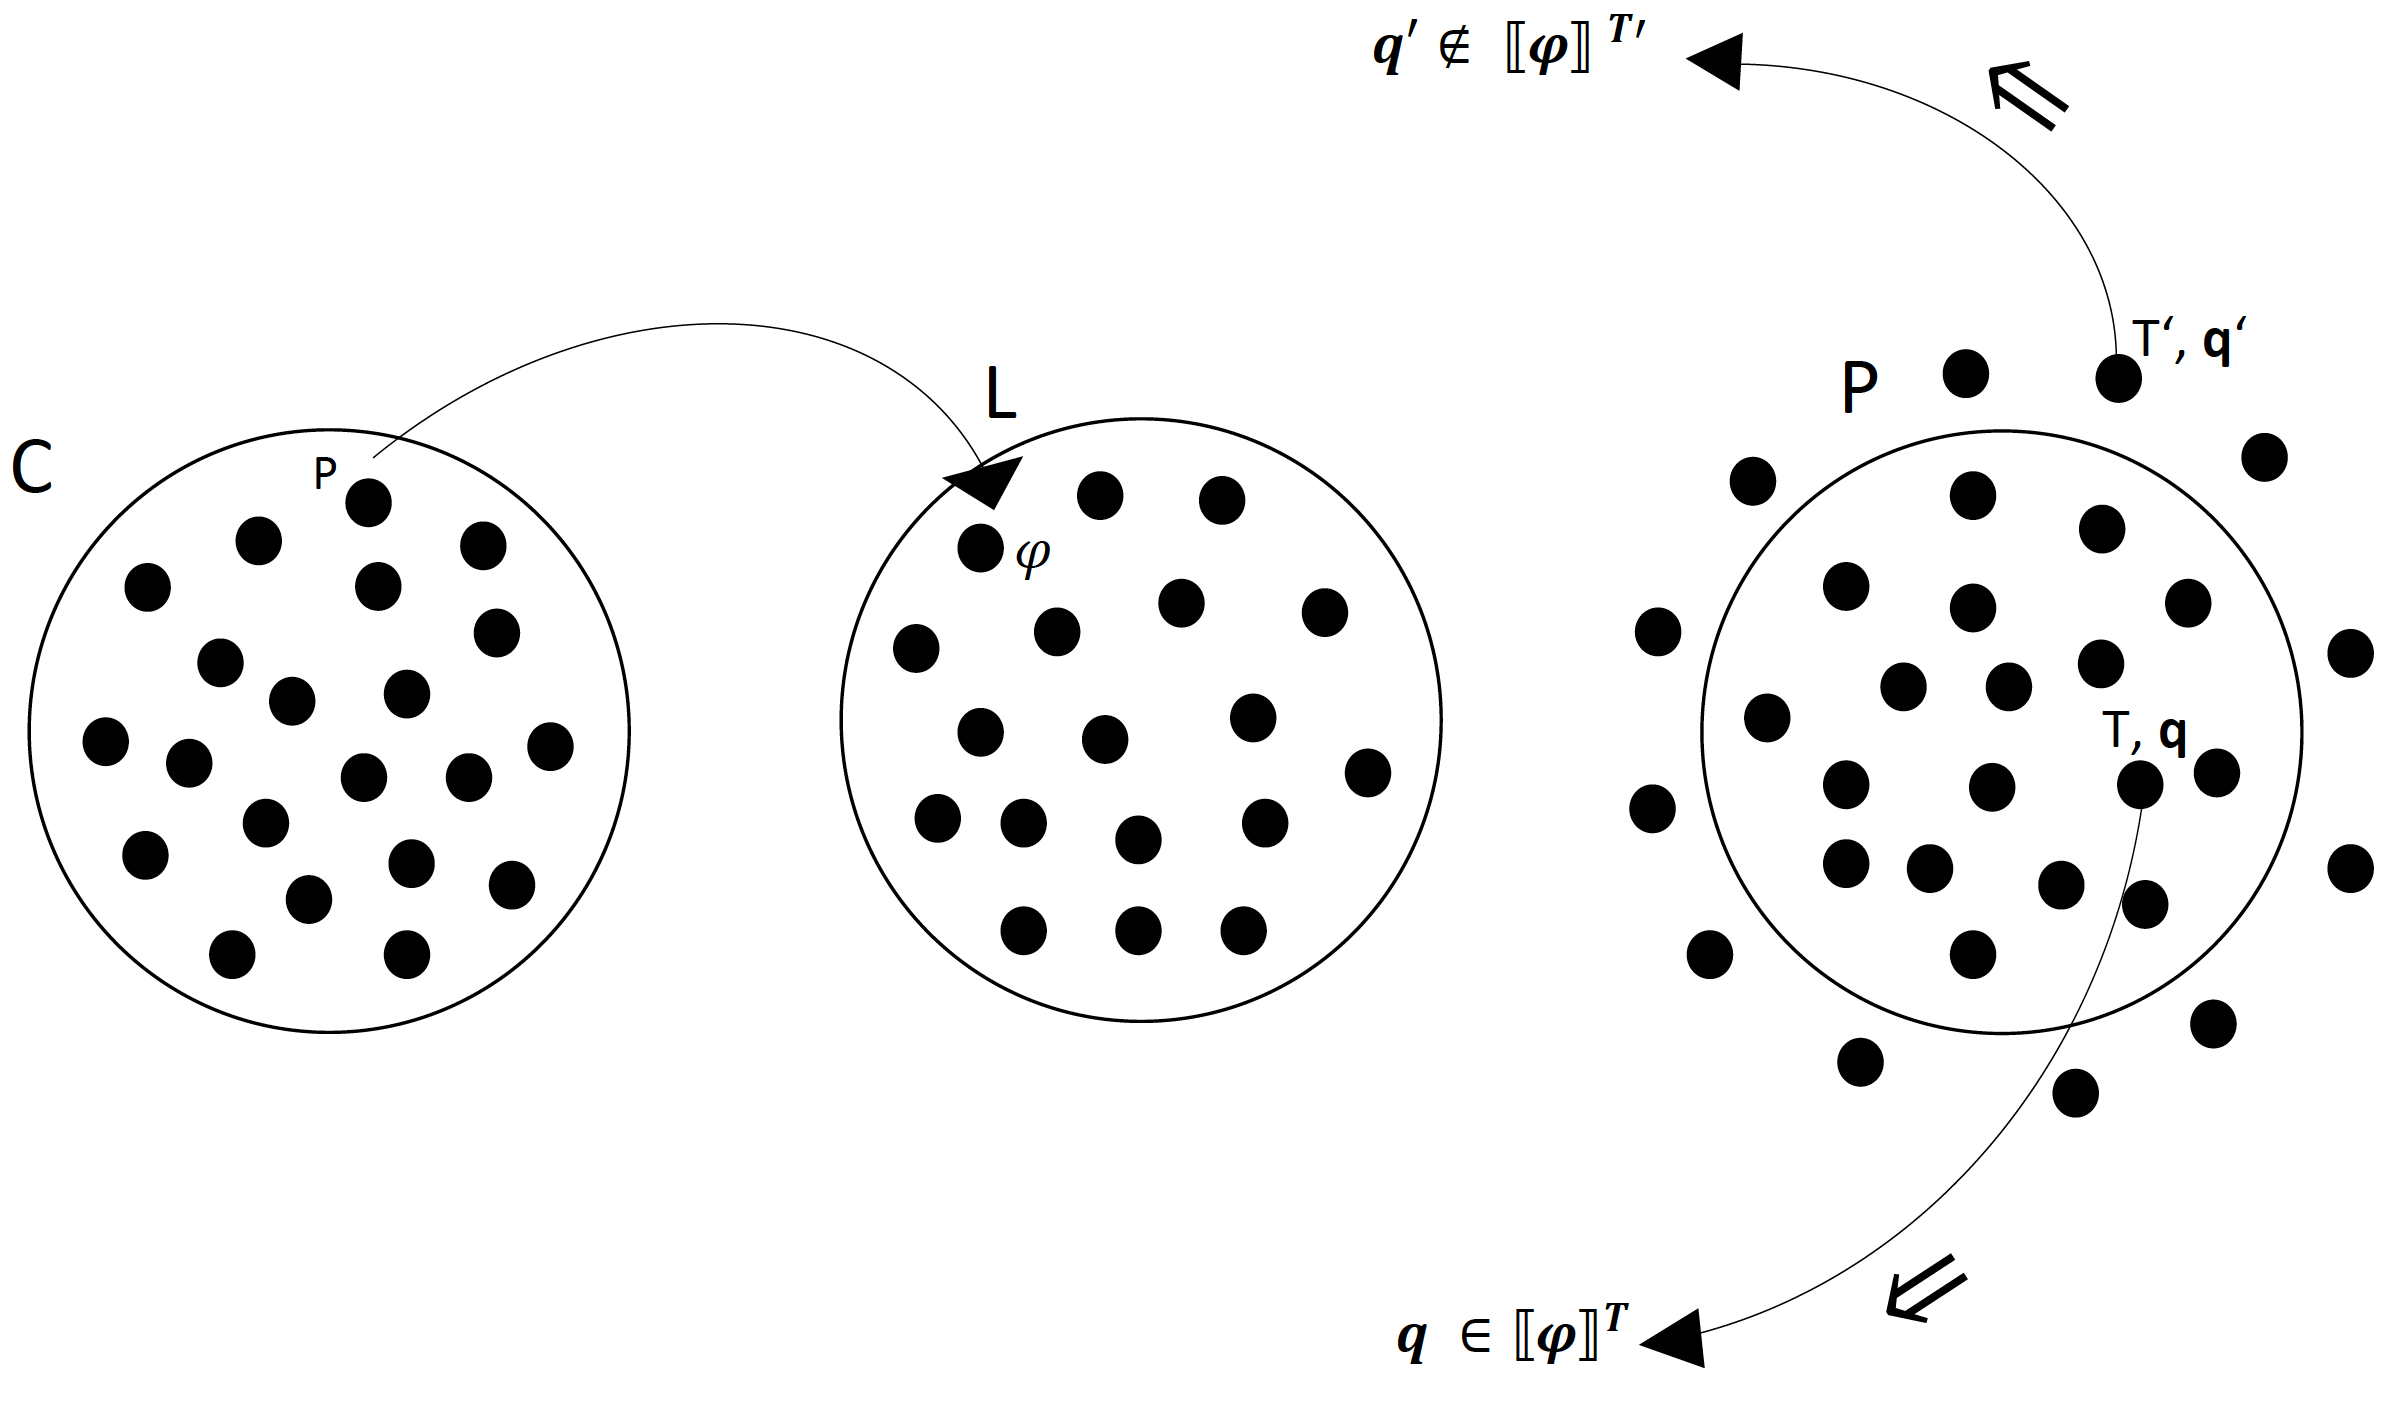
\includegraphics[width=0.9\textwidth]{logic-capture-class.png}}}
\end{figure}


\end{frame}

\section{PHFL}

\begin{frame}

	\begin{compactenum}[$\bullet$]
	\item PHFL is defined over LTS
	\item<2-> Elements of base type are elements of $\mathcal{P}(Q^d)$
	\item<3-> Higher order types are functions, functions of functions, $\dots$
	\end{compactenum}	
	
      \onslide<4->\begin{align*}
             \Phi,\Psi\Coloneqq&\top \mid p_i \mid \Phi \vee \Psi \mid \neg \Phi \mid \langle a \rangle_i \Phi \mid
        \{\emph{j}\,\} \Phi \mid X \mid 
        \\&\lambda (X^v\colon\tau).\Phi \mid \Phi\,\Psi\mid  \mu (X\colon\tau).\Phi
        \end{align*}

\begin{multicols}{3}
  \onslide<5->\begin{equation}
    \lambda (X^v\colon\tau).X
  \end{equation}\break
  \onslide<6->\begin{equation}
    \lambda (X^v\colon\tau).\top
  \end{equation}\break
  \onslide<7->\begin{equation}
    \lambda (X^v\colon\bullet).\top\,\top
  \end{equation}
\end{multicols}
\end{frame}

\begin{frame}

   Consider ${\color<4,11>[rgb]{1,0,0}\big({\color<6,8>[rgb]{1,0,0}{\color<2>[rgb]{1,0,0}\nu F}.\,
        {\color<3>[rgb]{1,0,0} {\color<13>[rgb]{1,0,0}\lambda{\color<12>[rgb]{1,0,0}X}.\, \lambda {\color<12>[rgb]{1,0,0}Y}.\, \,{\color<4>[rgb]{1,0,0} ({\color<12>[rgb]{1,0,0}X} \Leftrightarrow {\color<12>[rgb]{1,0,0}Y}) \wedge
        \underset{{\color<12>[rgb]{1,0,0}a} \in \Sigma}{\bigwedge}}}{\color<4>[rgb]{1,0,0}  {\color<9>[rgb]{1,0,0}F} {\color<13>[rgb]{1,0,0}\langle {\color<12>[rgb]{1,0,0}a} \rangle_1 {\color<12>[rgb]{1,0,0}X} \langle {\color<12>[rgb]{1,0,0}a} \rangle_2 {\color<12>[rgb]{1,0,0}Y}}}}}\big)}{\color<5>[rgb]{1,0,0}\top \top}$
    \\ \onslide<7->Unfold
   {\onslide<10->\begin{align*}
        \big(
        {\color<13,14>[rgb]{1,0,0}\lambda {\color<16>[rgb]{1,0,0}X}.}\, & {\color<13>[rgb]{1,0,0}{\color<15>[rgb]{1,0,0}\lambda {\color<17>[rgb]{1,0,0}Y}.}\, (X \Leftrightarrow Y) \wedge
        \underset{a \in \Sigma}{\bigwedge}} {\color<11>[rgb]{1,0,0}\big(\nu F .\,
        \lambda {\color<12>[rgb]{1,0,0}X'}.\, \lambda {\color<12>[rgb]{1,0,0}Y'}.\, ({\color<12>[rgb]{1,0,0}X'} \Leftrightarrow {\color<12>[rgb]{1,0,0}Y'})}\\& {\color<11>[rgb]{1,0,0}\wedge
        \underset{{\color<12>[rgb]{1,0,0}b} \in \Sigma}{\bigwedge} F \langle{\color<12>[rgb]{1,0,0} b} \rangle_1 {\color<12>[rgb]{1,0,0}X'} \langle {\color<12>[rgb]{1,0,0}b} \rangle_2 {\color<12>[rgb]{1,0,0}Y'}\big)} {\color<13>[rgb]{1,0,0}\langle a \rangle_1 X \langle a \rangle_2 Y}\big){\color<16,20>[rgb]{1,0,0}\top} {\color<17,21>[rgb]{1,0,0}\top}
    \end{align*}}
   \onslide<18-> Substitute
       \onslide<19->\begin{align*}
        ({\color<20>[rgb]{1,0,0}\top} &\Leftrightarrow {\color<21>[rgb]{1,0,0}\top}) \wedge
        \underset{a \in \Sigma}{\bigwedge} \big(\nu F .\,
        \lambda X'.\, \lambda Y'.\, (X' \Leftrightarrow Y')\\& \wedge
        \underset{b \in \Sigma}{\bigwedge} F \langle b \rangle_1 X' \langle b \rangle_2 Y'\big)\langle a \rangle_1 {\color<20>[rgb]{1,0,0}\top} \langle a \rangle_2 {\color<21>[rgb]{1,0,0}\top}
    \end{align*}

\end{frame}
\begin{frame}
    
        \begin{align*}
         (\top &\Leftrightarrow \top) \wedge
        \underset{a \in \Sigma}{\bigwedge} {\color<3>[rgb]{1,0,0}\big(\nu F .\,
        {\color<7>[rgb]{1,0,0}\lambda {\color<6>[rgb]{1,0,0}X'}.\, \lambda {\color<6>[rgb]{1,0,0}Y'}.\, ({\color<6>[rgb]{1,0,0}X'} \Leftrightarrow {\color<6>[rgb]{1,0,0}Y'}) \wedge
        \underset{b \in \Sigma}{\bigwedge}} {\color<4>[rgb]{1,0,0}F} {\color<7>[rgb]{1,0,0}\langle {\color<6>[rgb]{1,0,0}b} \rangle_1 {\color<6>[rgb]{1,0,0}X'} \langle {\color<6>[rgb]{1,0,0}b} \rangle_2 {\color<6>[rgb]{1,0,0}Y'}}\big)}\\&\langle a \rangle_1 \top \langle a \rangle_2 \top
    \end{align*}
   \onslide<2-> Unfold
   \onslide<5->\begin{align*}
        (\top &\Leftrightarrow \top) \wedge
        \underset{a \in \Sigma}{\bigwedge} \big(
        {\color<7>[rgb]{1,0,0}{\color<8>[rgb]{1,0,0}\lambda {\color<10>[rgb]{1,0,0}X'}}.\, {\color<9>[rgb]{1,0,0}\lambda {\color<11>[rgb]{1,0,0}Y'}}.\, (X' \Leftrightarrow Y') \wedge
        \underset{b \in \Sigma}{\bigwedge}} \big(\nu F.\,
        \lambda {\color<6>[rgb]{1,0,0}X''}.\, \lambda {\color<6>[rgb]{1,0,0}Y''}.\, \\&({\color<6>[rgb]{1,0,0}X''} \Leftrightarrow {\color<6>[rgb]{1,0,0}Y''}) \wedge
        \underset{c \in \Sigma}{\bigwedge} F \langle {\color<6>[rgb]{1,0,0}c} \rangle_1 {\color<6>[rgb]{1,0,0}X''} \langle {\color<6>[rgb]{1,0,0}c} \rangle_2 {\color<6>[rgb]{1,0,0}Y''}\big) {\color<7>[rgb]{1,0,0}\langle b \rangle_1 X' \langle b \rangle_2 Y'}\big){\color<10,14>[rgb]{1,0,0}\langle a \rangle_1 \top} {\color<11,15>[rgb]{1,0,0}\langle a \rangle_2 \top}
    \end{align*}
    \onslide<12->Substitute
       \onslide<13->\begin{align*}
        (\top &\Leftrightarrow \top) \wedge
        \underset{a \in \Sigma}{\bigwedge} 
        ({\color<14>[rgb]{1,0,0}\langle a \rangle_1 \top} \Leftrightarrow {\color<15>[rgb]{1,0,0}\langle a \rangle_2 \top}) \wedge
        \underset{b \in \Sigma}{\bigwedge} \big(\nu F.\,
        \lambda X''.\, \lambda Y''.\, \\&(X'' \Leftrightarrow Y'') \wedge
        \underset{c \in \Sigma}{\bigwedge} F \langle c \rangle_1 X'' \langle c \rangle_2 Y''\big) {\color<14>[rgb]{1,0,0}\langle ba \rangle_1 \top} {\color<15>[rgb]{1,0,0}\langle ba \rangle_2 \top} 
    \end{align*}

\end{frame}
\begin{frame}
       \begin{align*}
        &\big( (\top \Leftrightarrow \top) \wedge
        \underset{a \in \Sigma}{\bigwedge} \big(
        (\langle a \rangle_1 \top \Leftrightarrow \langle a \rangle_2 \top) \wedge
        \underset{b \in \Sigma}{\bigwedge} \big(\nu F.\,
        \lambda X''.\, \lambda Y''.\, \\&(X'' \Leftrightarrow Y'') \wedge
        \underset{c \in \Sigma}{\bigwedge} F \langle c \rangle_1 X'' \langle c \rangle_2 Y''\big) \langle ba \rangle_1 \top \langle ba \rangle_2 \top \big)\big)
    \end{align*}
    \onslide<2->Continuing, we obtain
       \onslide<3->\begin{align*}
         \top &\Leftrightarrow \top \wedge \underset{a \in \Sigma}{\bigwedge} \langle a \rangle_1 \top \Leftrightarrow \langle a \rangle_2 \top \wedge \underset{b \in \Sigma}{\bigwedge}\langle ba \rangle_1 \top \Leftrightarrow \langle ba \rangle_2 \top \wedge \dots
        \\&
       \onslide<4->{ =\, \underset{w \in \Sigma^*}{\bigwedge} \langle w \rangle_1 \top \Leftrightarrow \langle w \rangle_2 \top}
    \end{align*}
    \onslide<5->trace equivalence.
\end{frame}

\section{How to}

\begin{frame}

\begin{figure}[ht]
	\centering{
  \only<1>{\hspace{-0.1cm}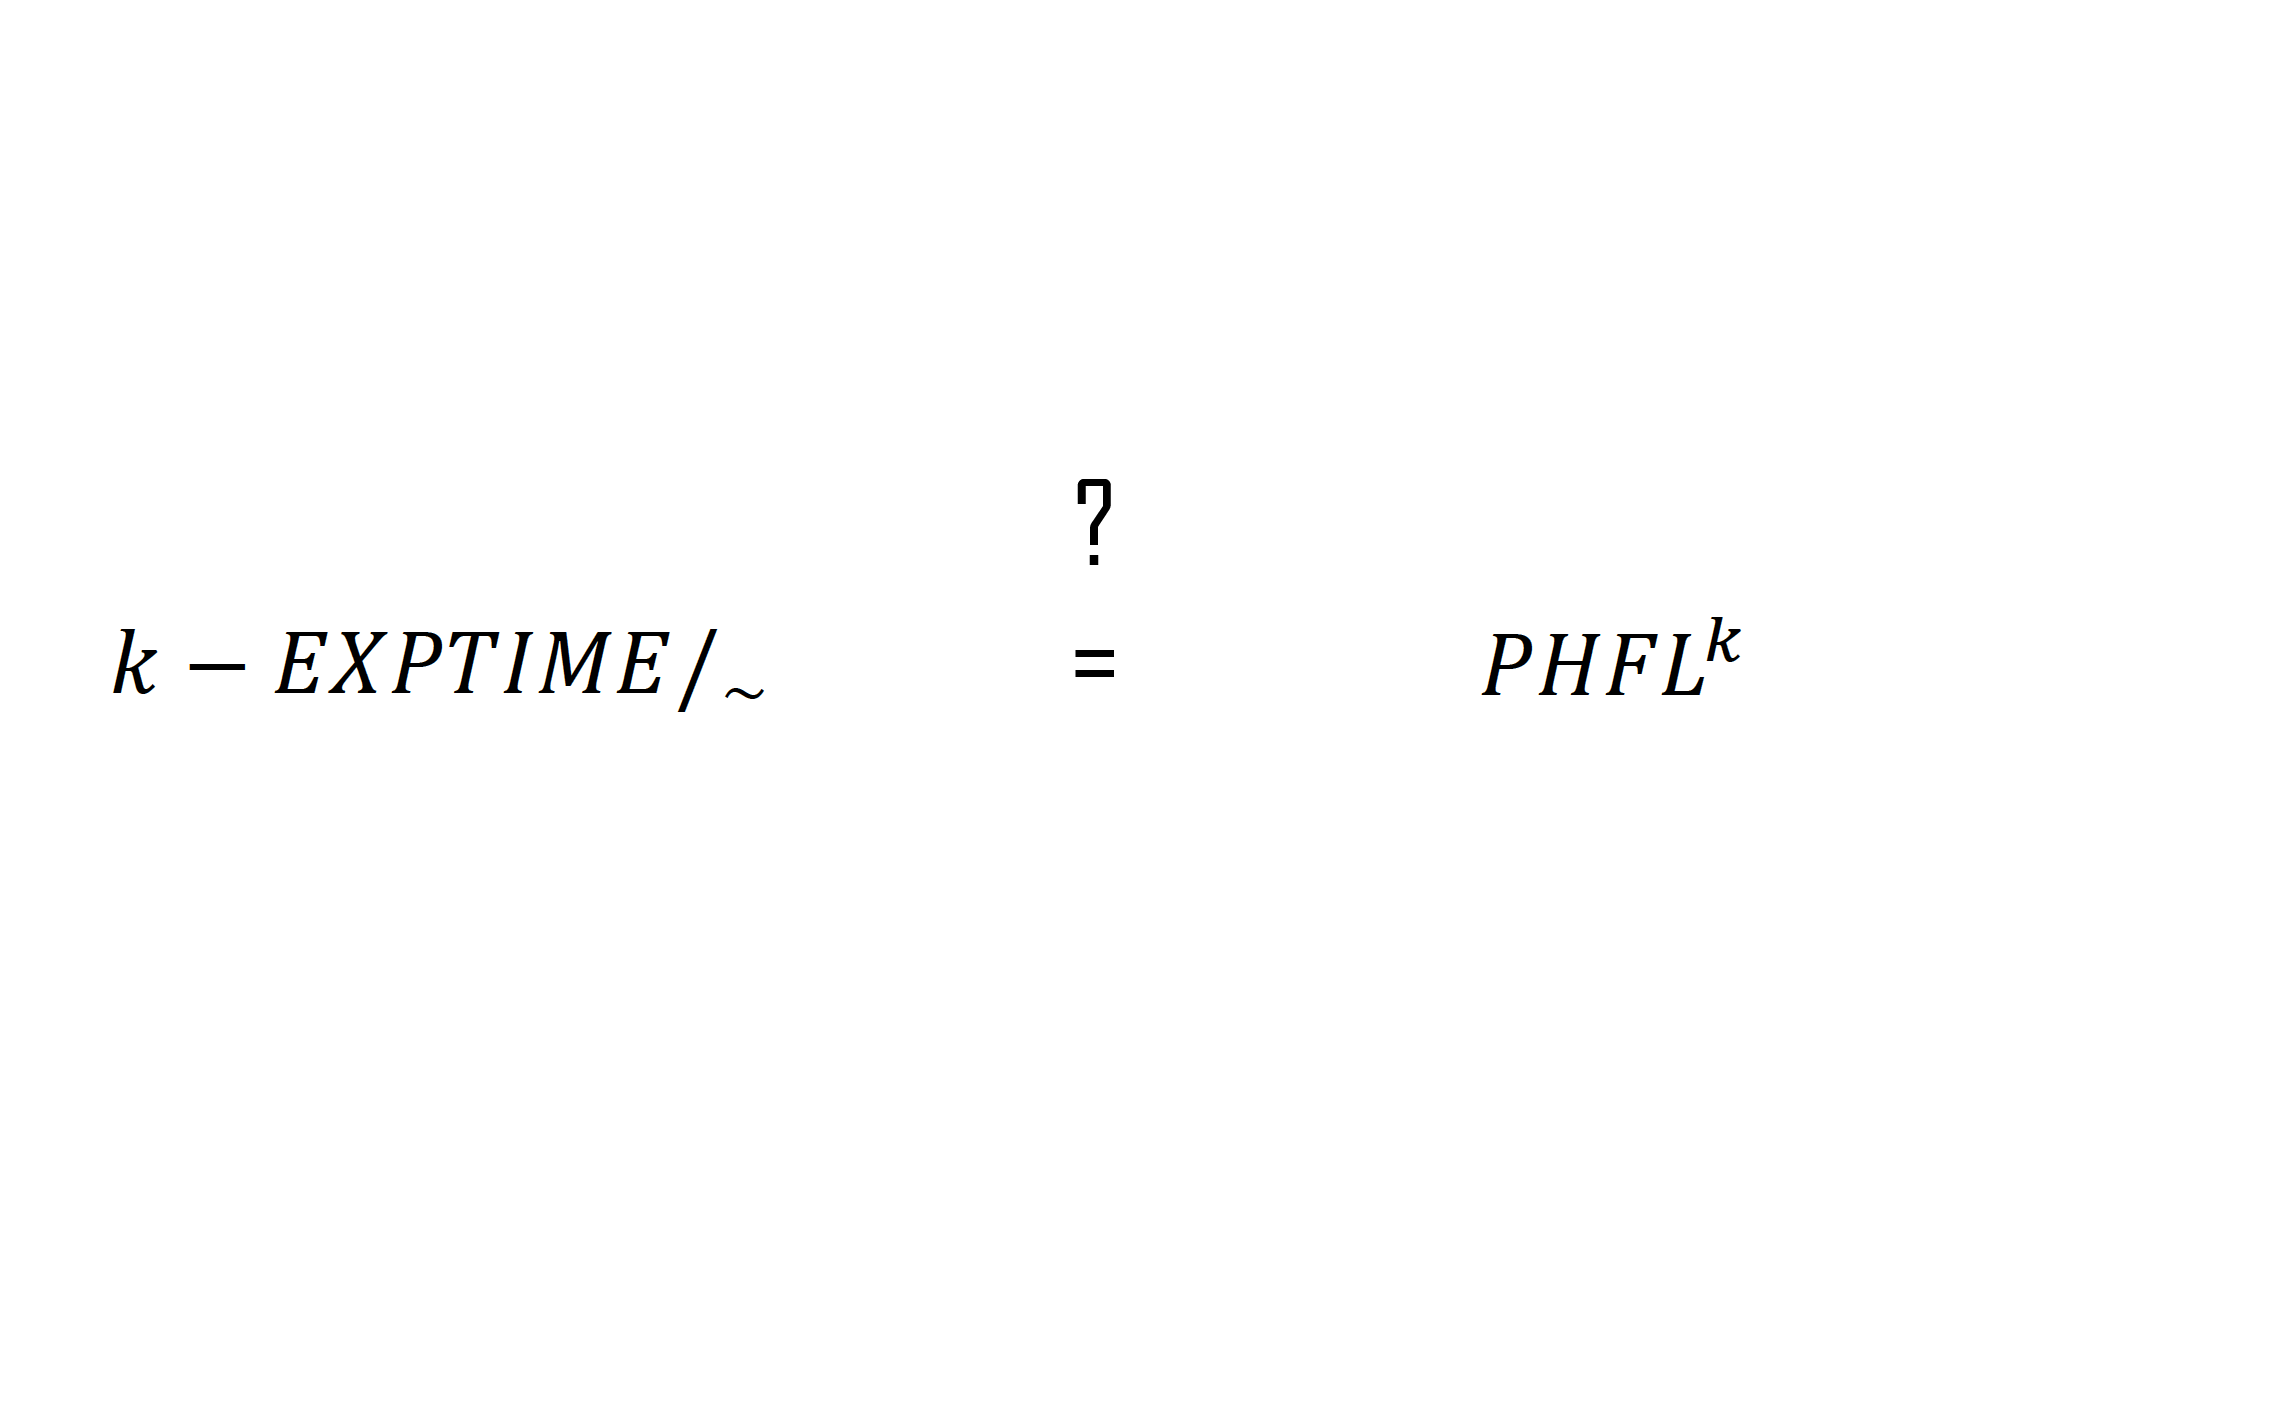
\includegraphics[width=0.9\textwidth]{phfl_0.png}}
  \only<2>{\hspace{-0.1cm}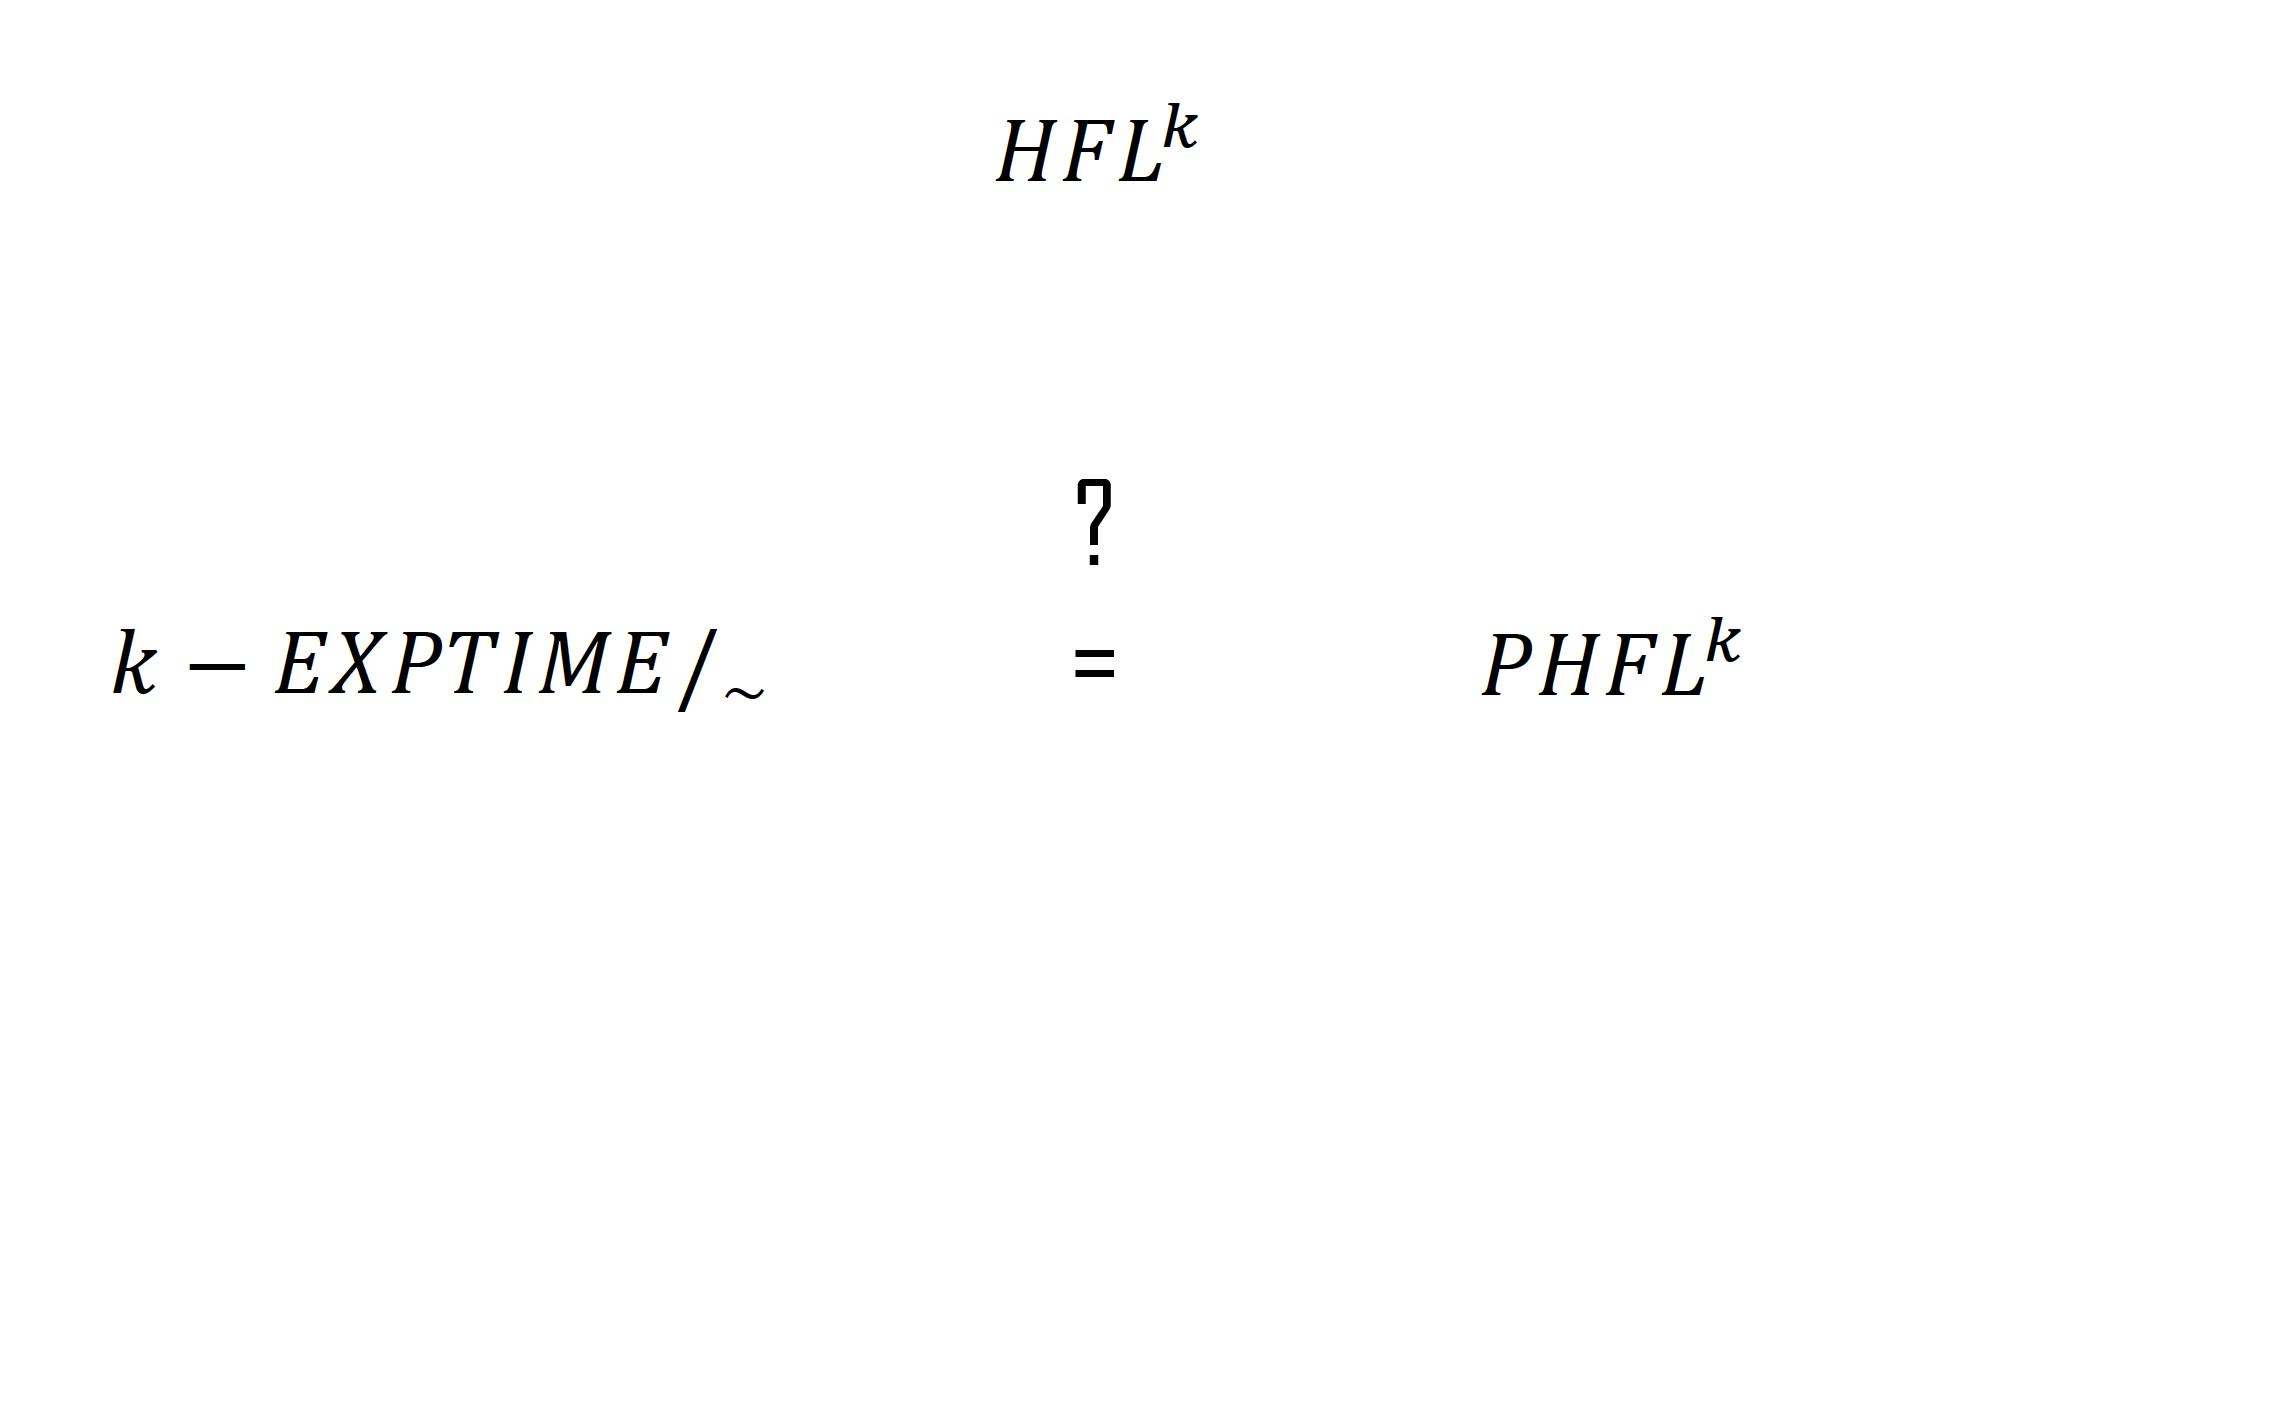
\includegraphics[width=0.9\textwidth]{phfl_1.png}}
  \only<3>{\hspace{-0.2cm}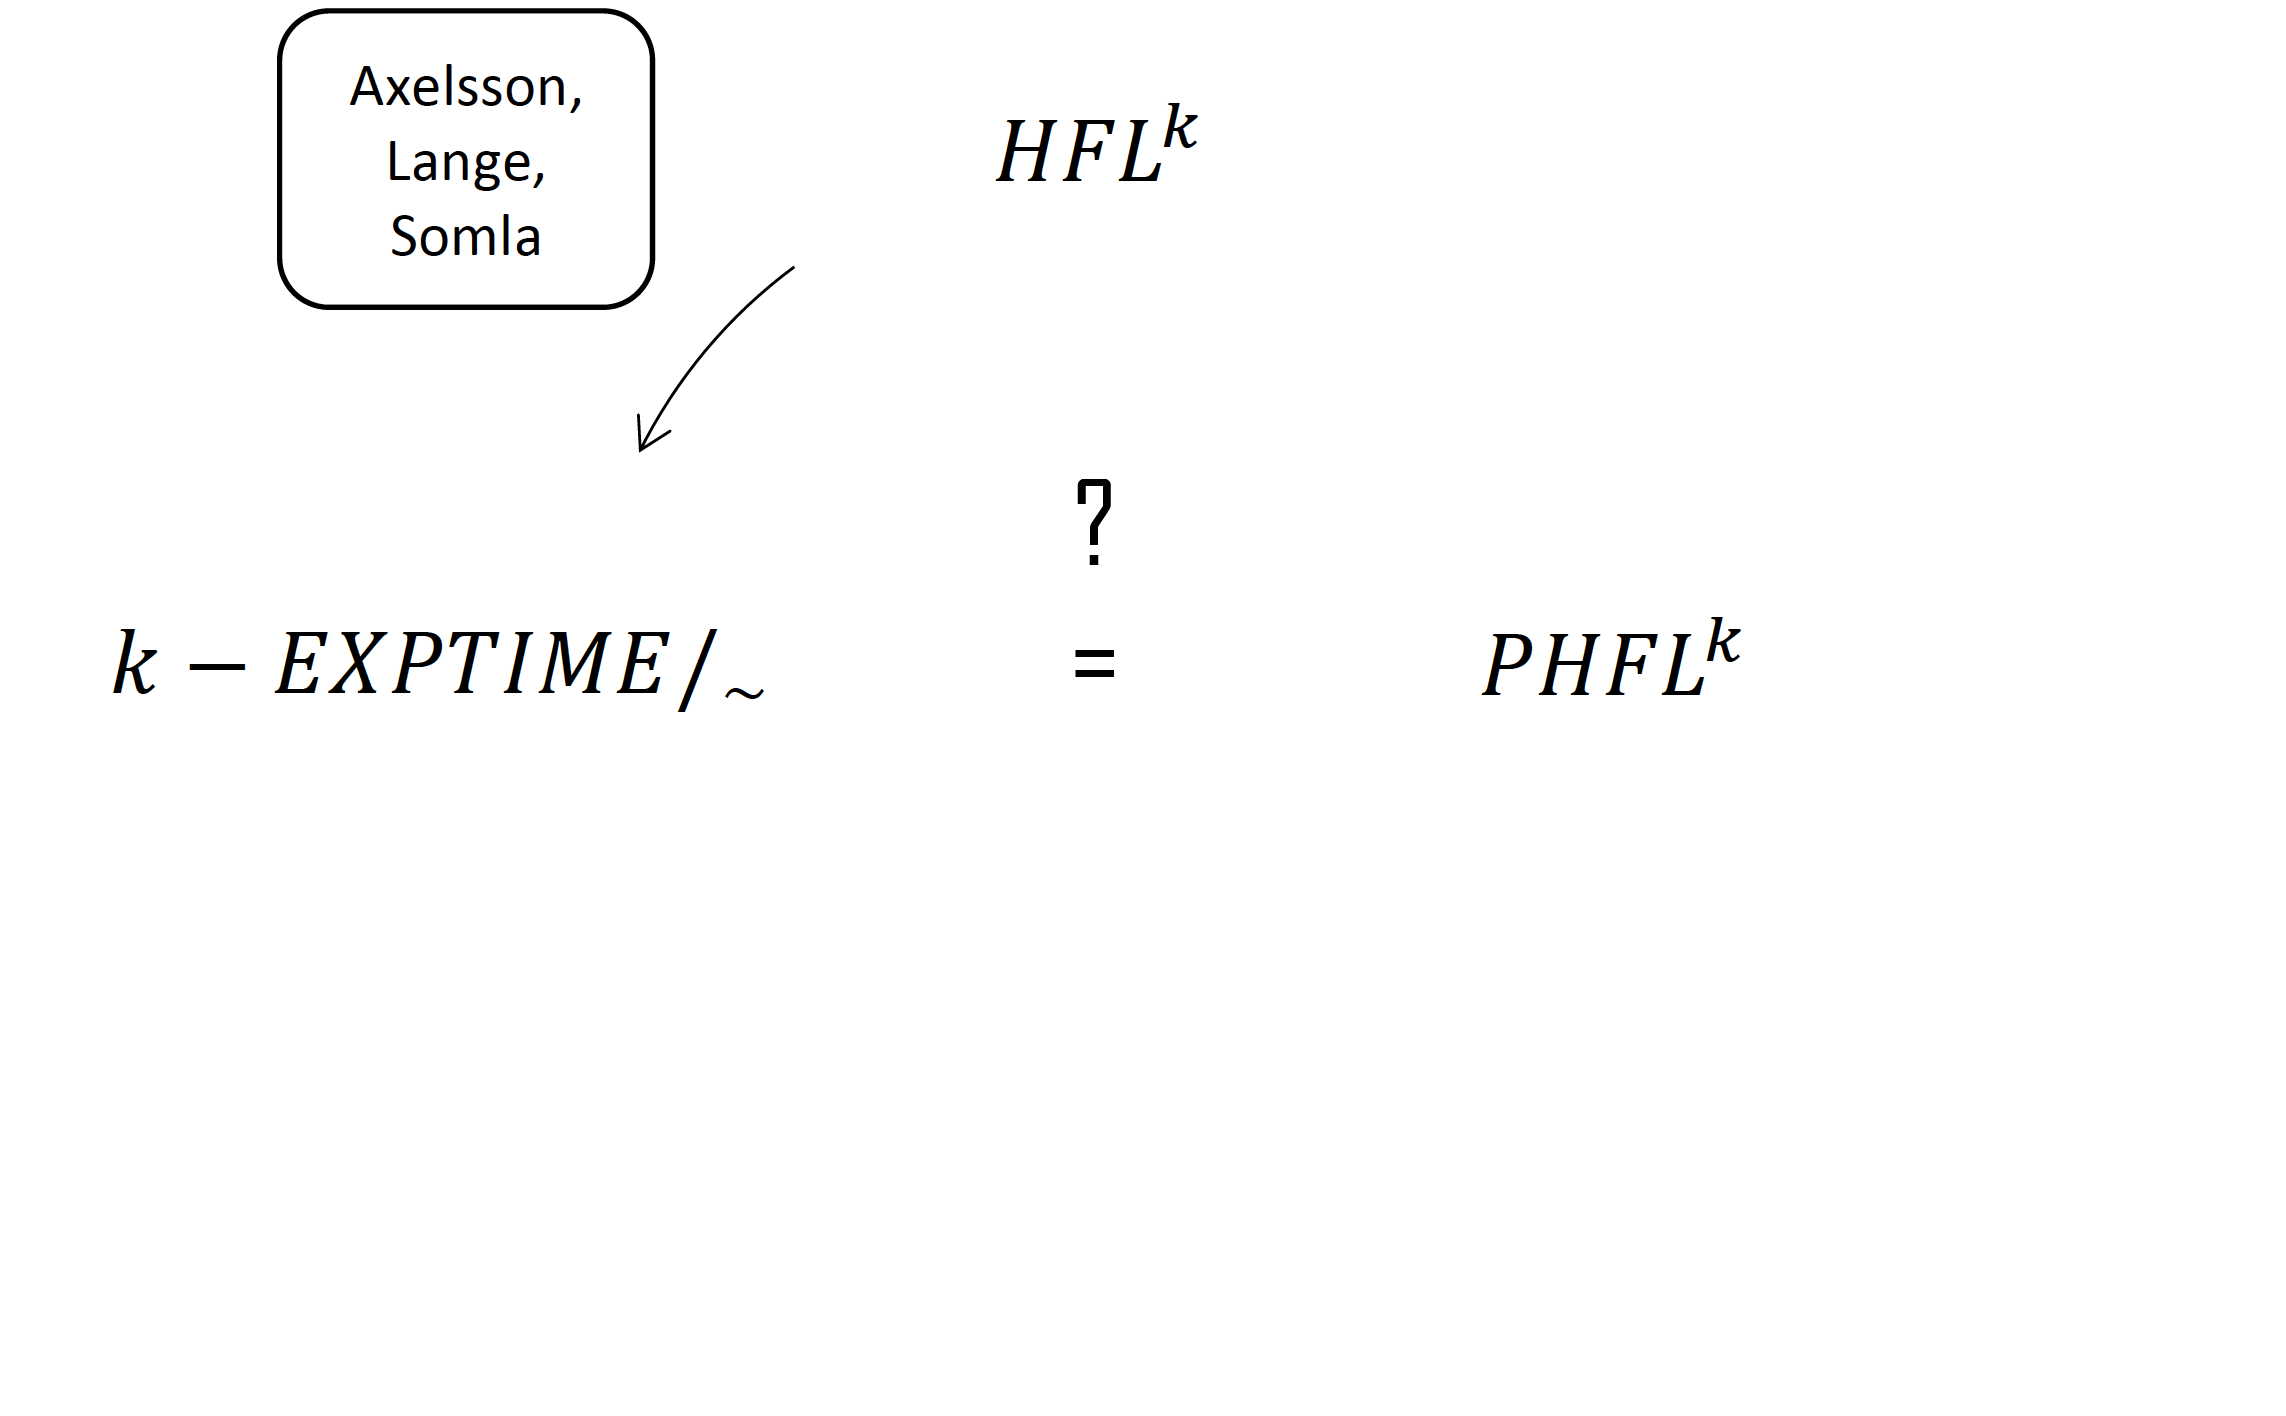
\includegraphics[width=0.9\textwidth]{phfl_2.png}}
   \only<4>{\hspace{-0.3cm}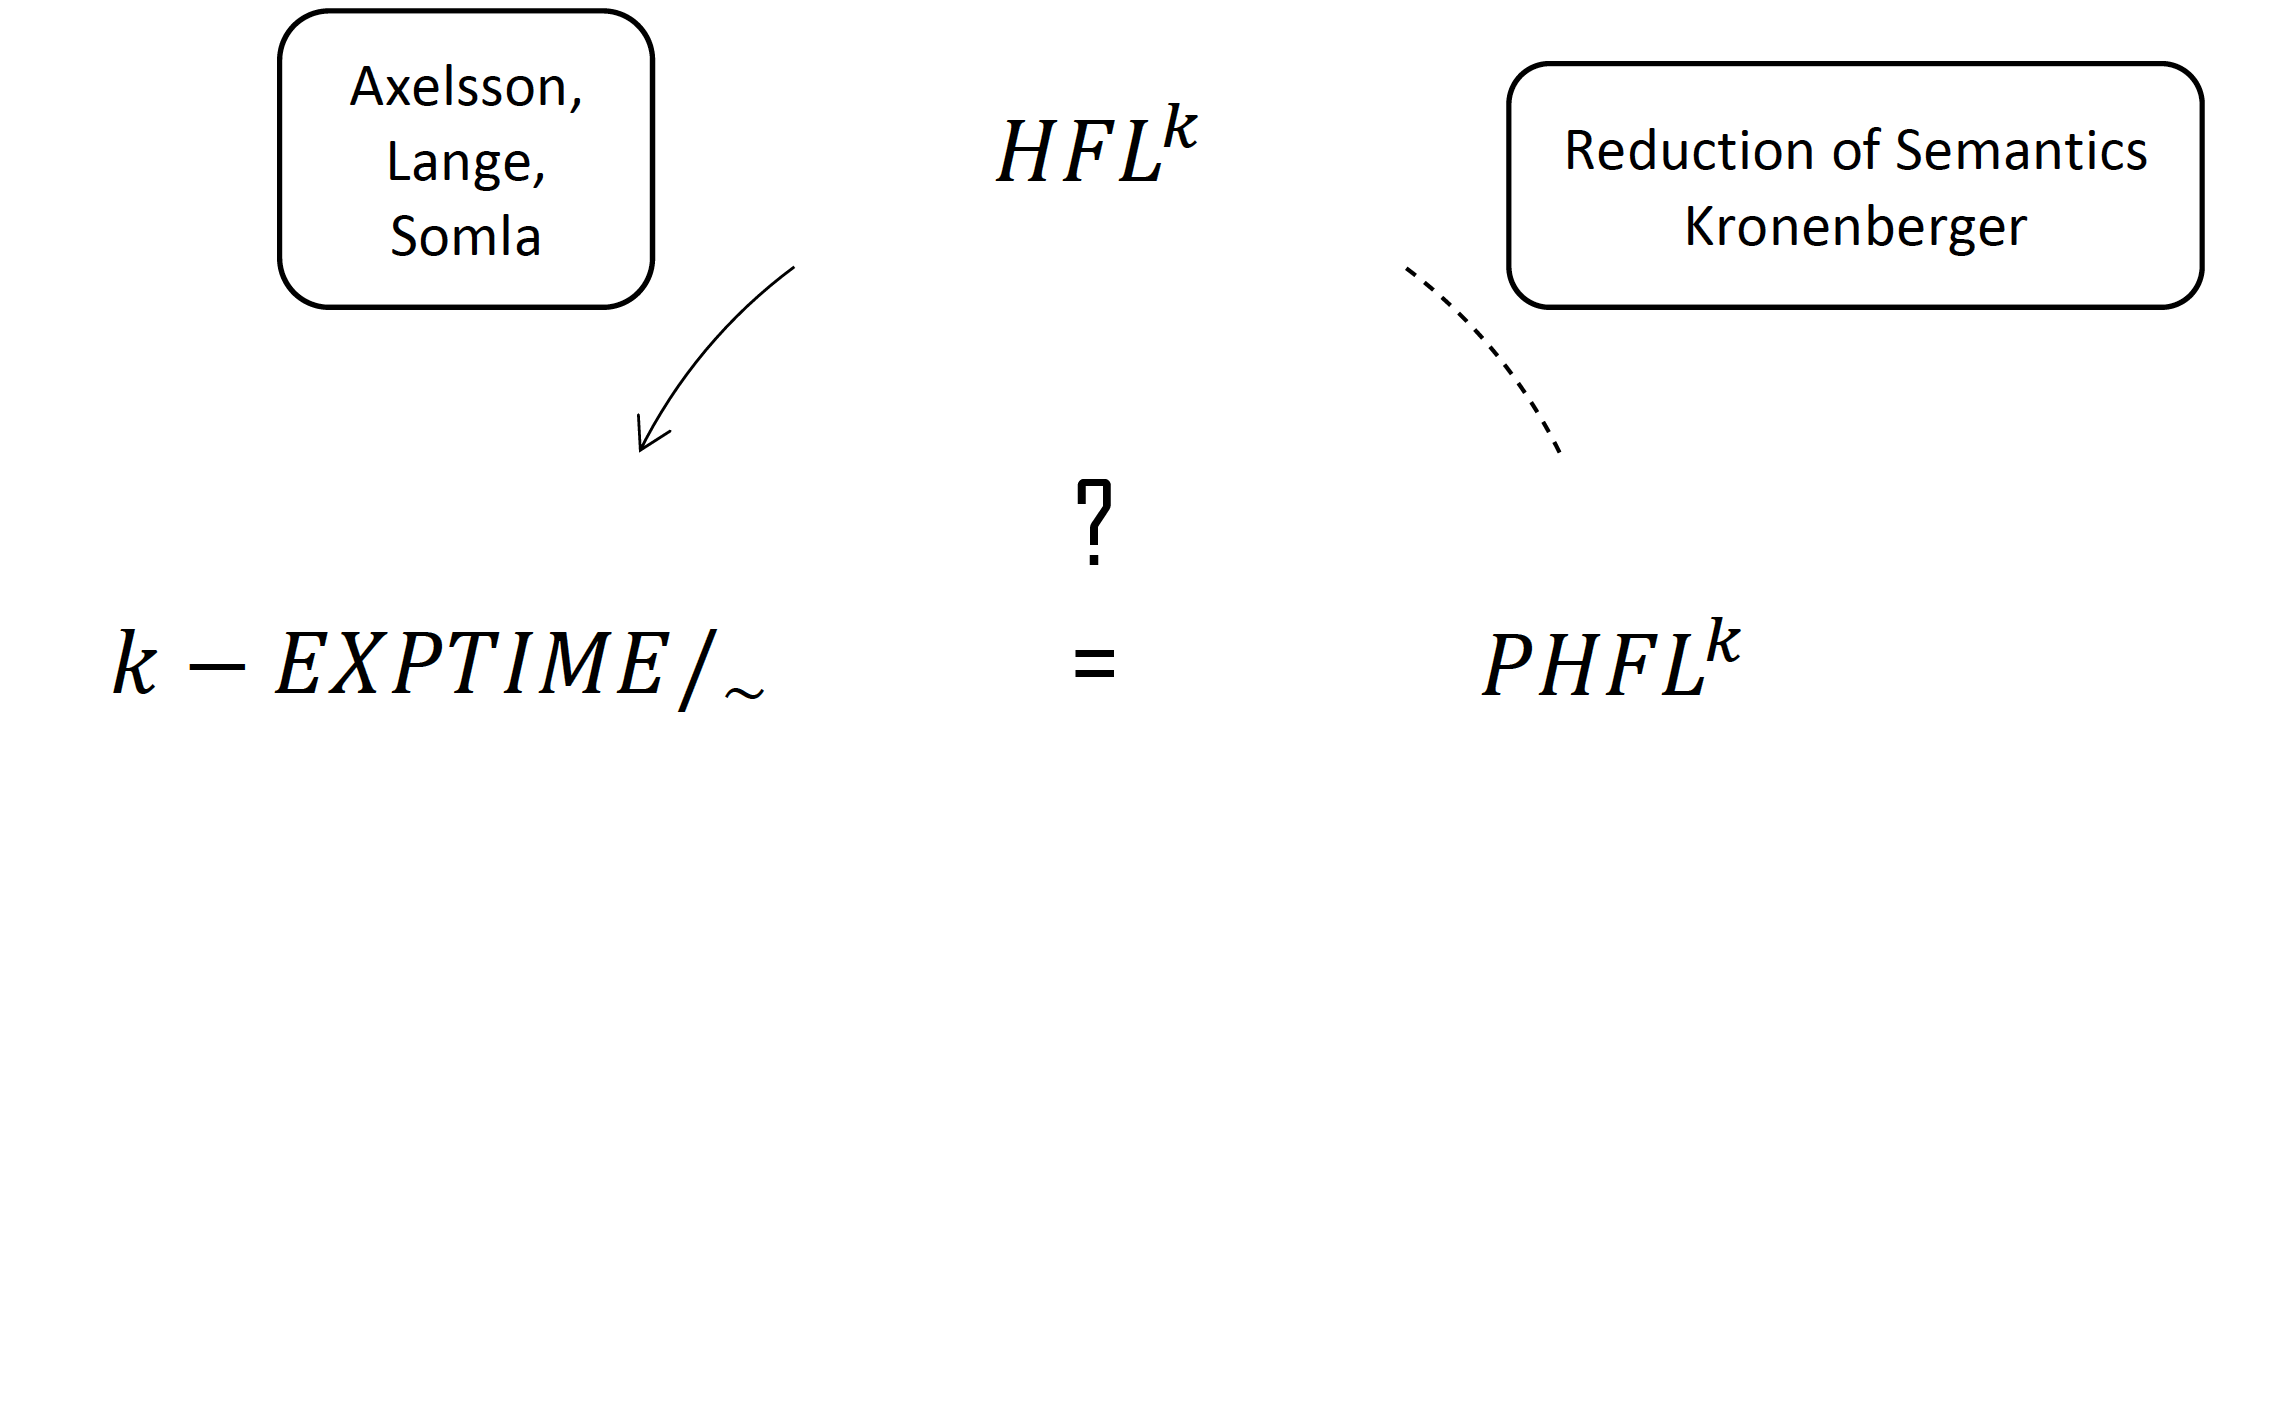
\includegraphics[width=0.9\textwidth]{phfl_3.png}}
  \only<5>{\hspace{-0.4cm}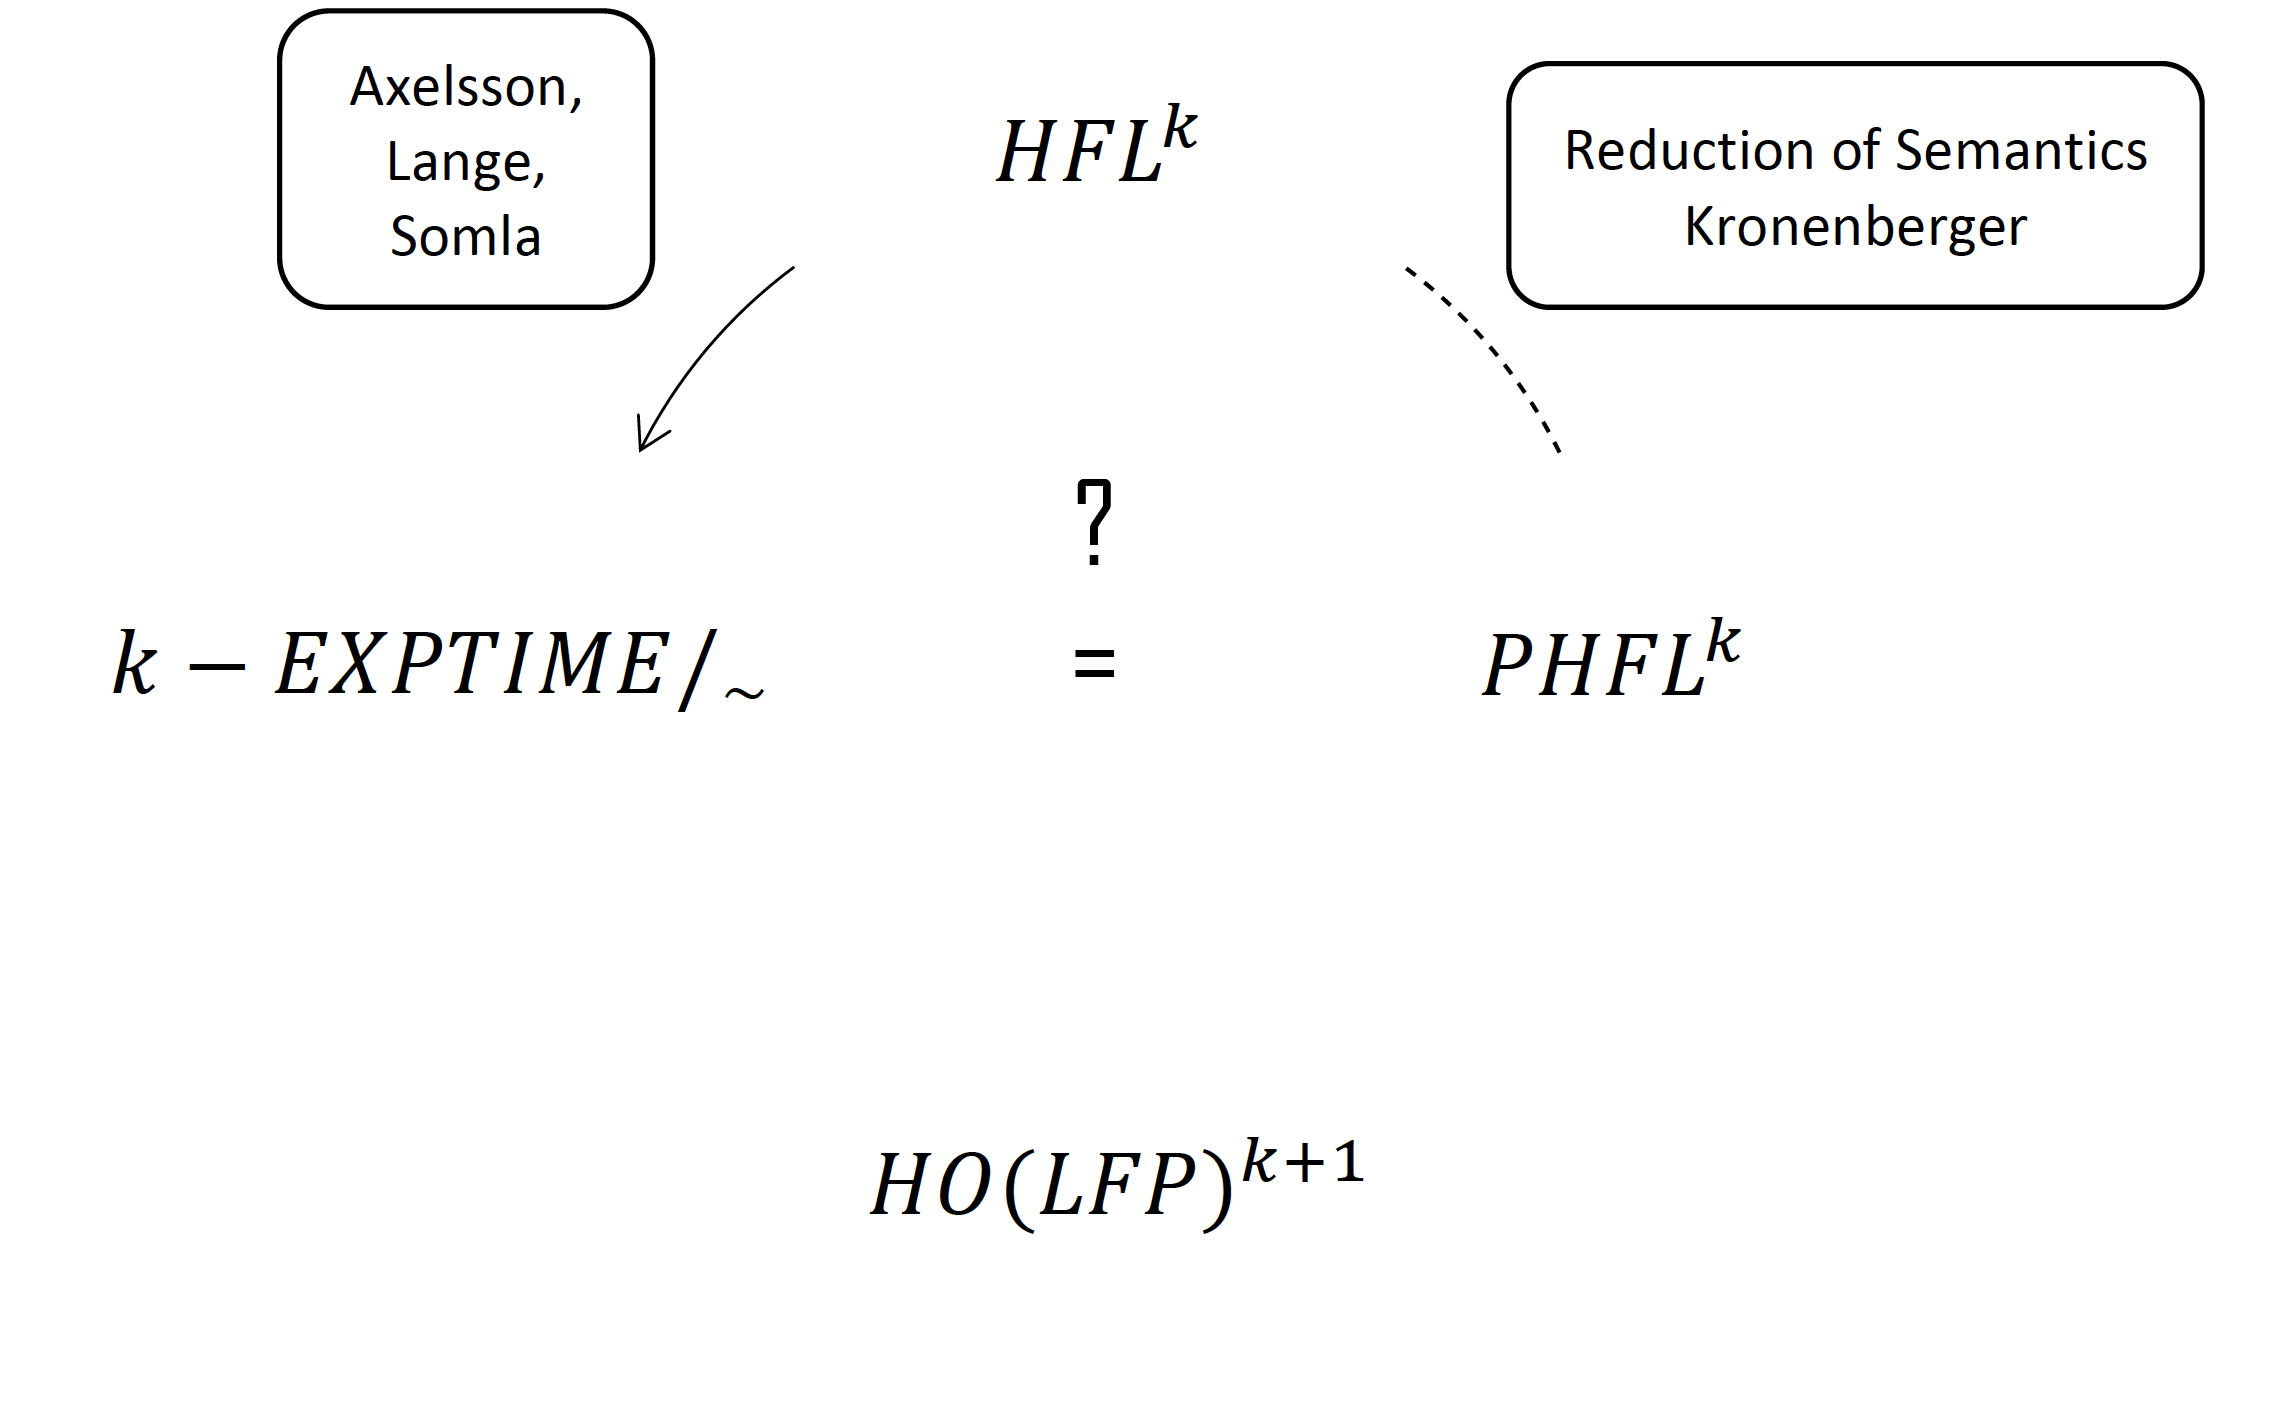
\includegraphics[width=0.9\textwidth]{phfl_4.png}}
  \only<6>{\hspace{-0.5cm}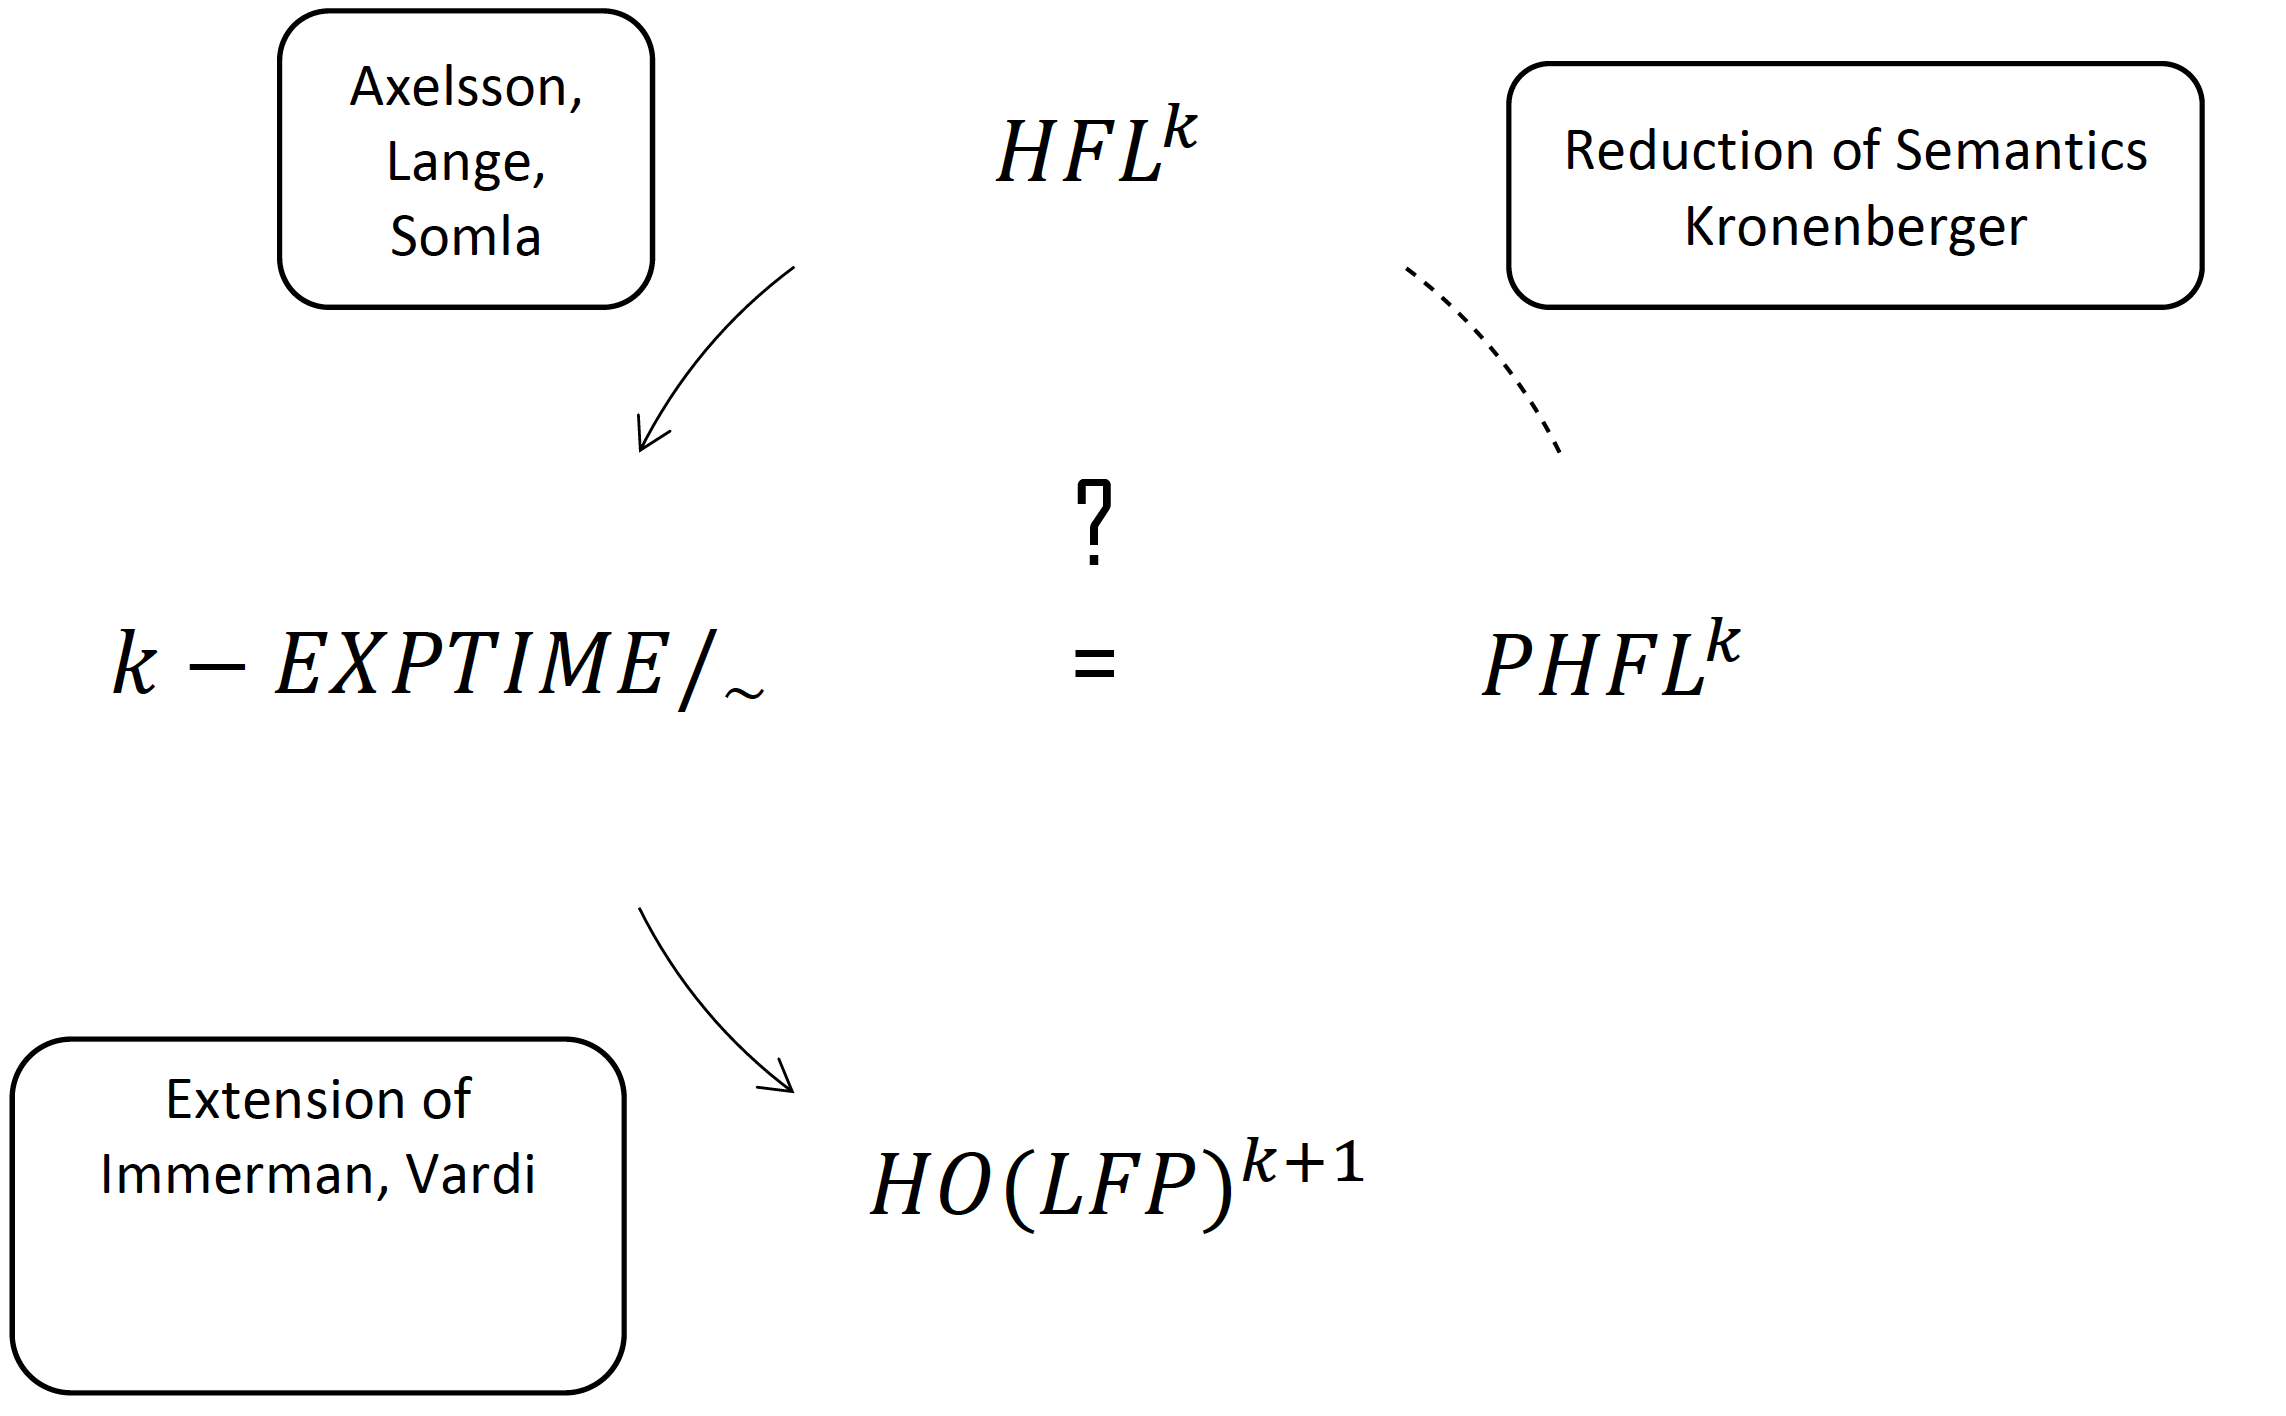
\includegraphics[width=0.9\textwidth]{phfl_5.png}}
  \only<7>{\hspace{-0.6cm}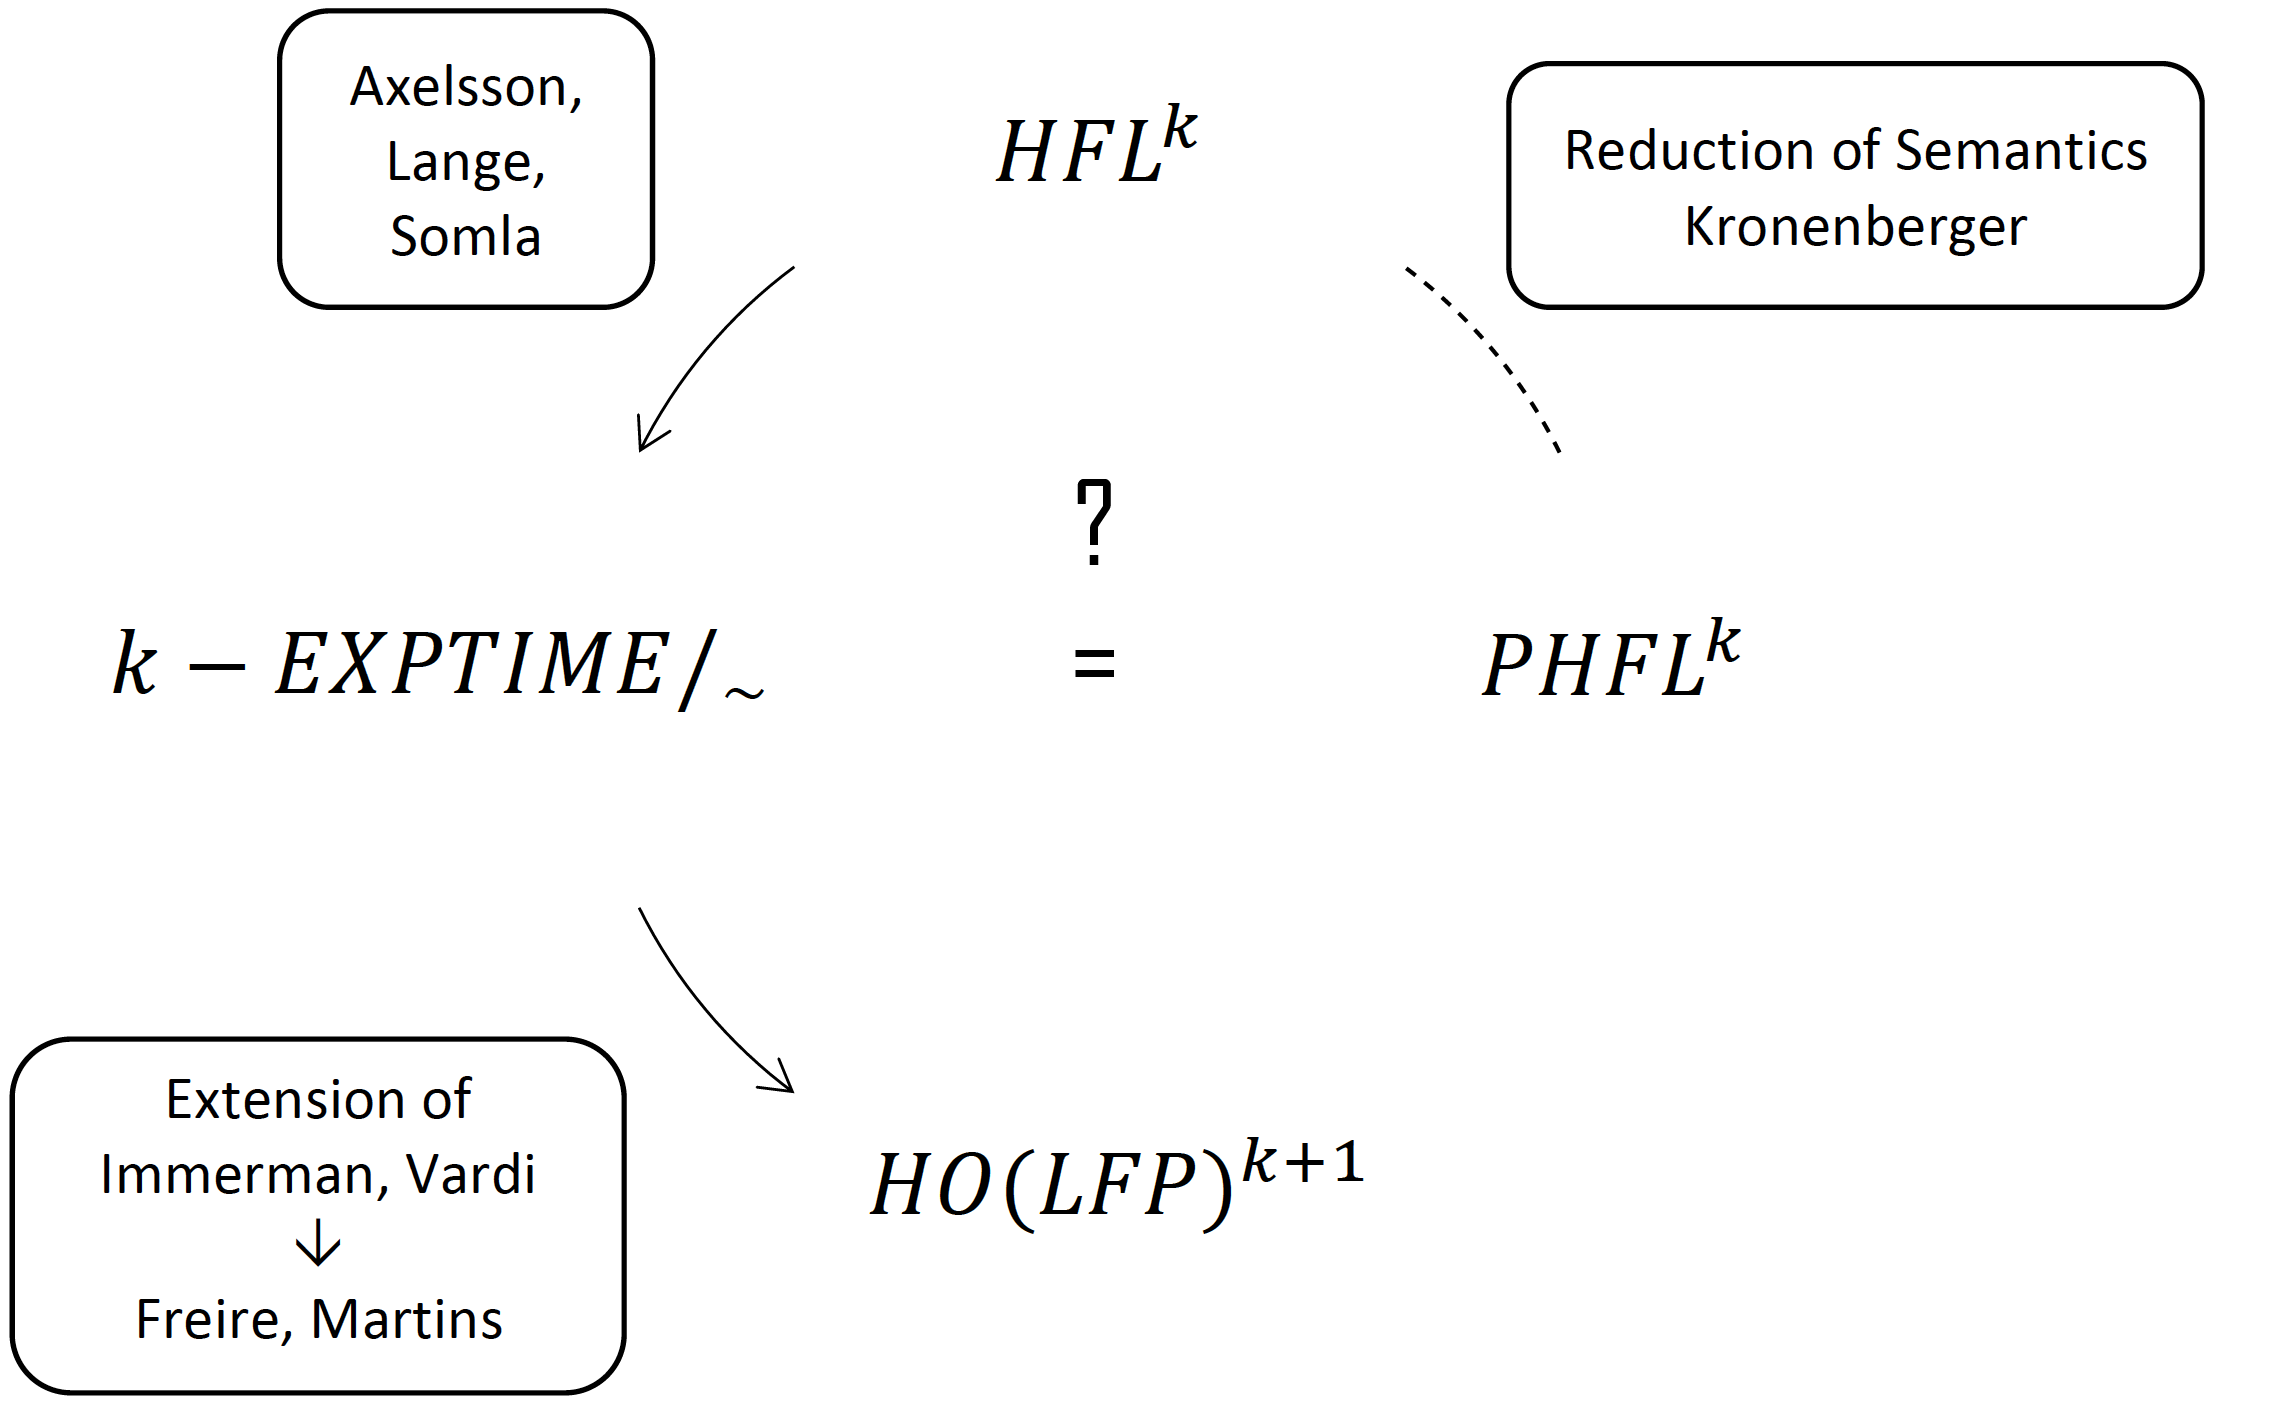
\includegraphics[width=0.9\textwidth]{phfl_6.png}}
  \only<8>{\hspace{-0.7cm}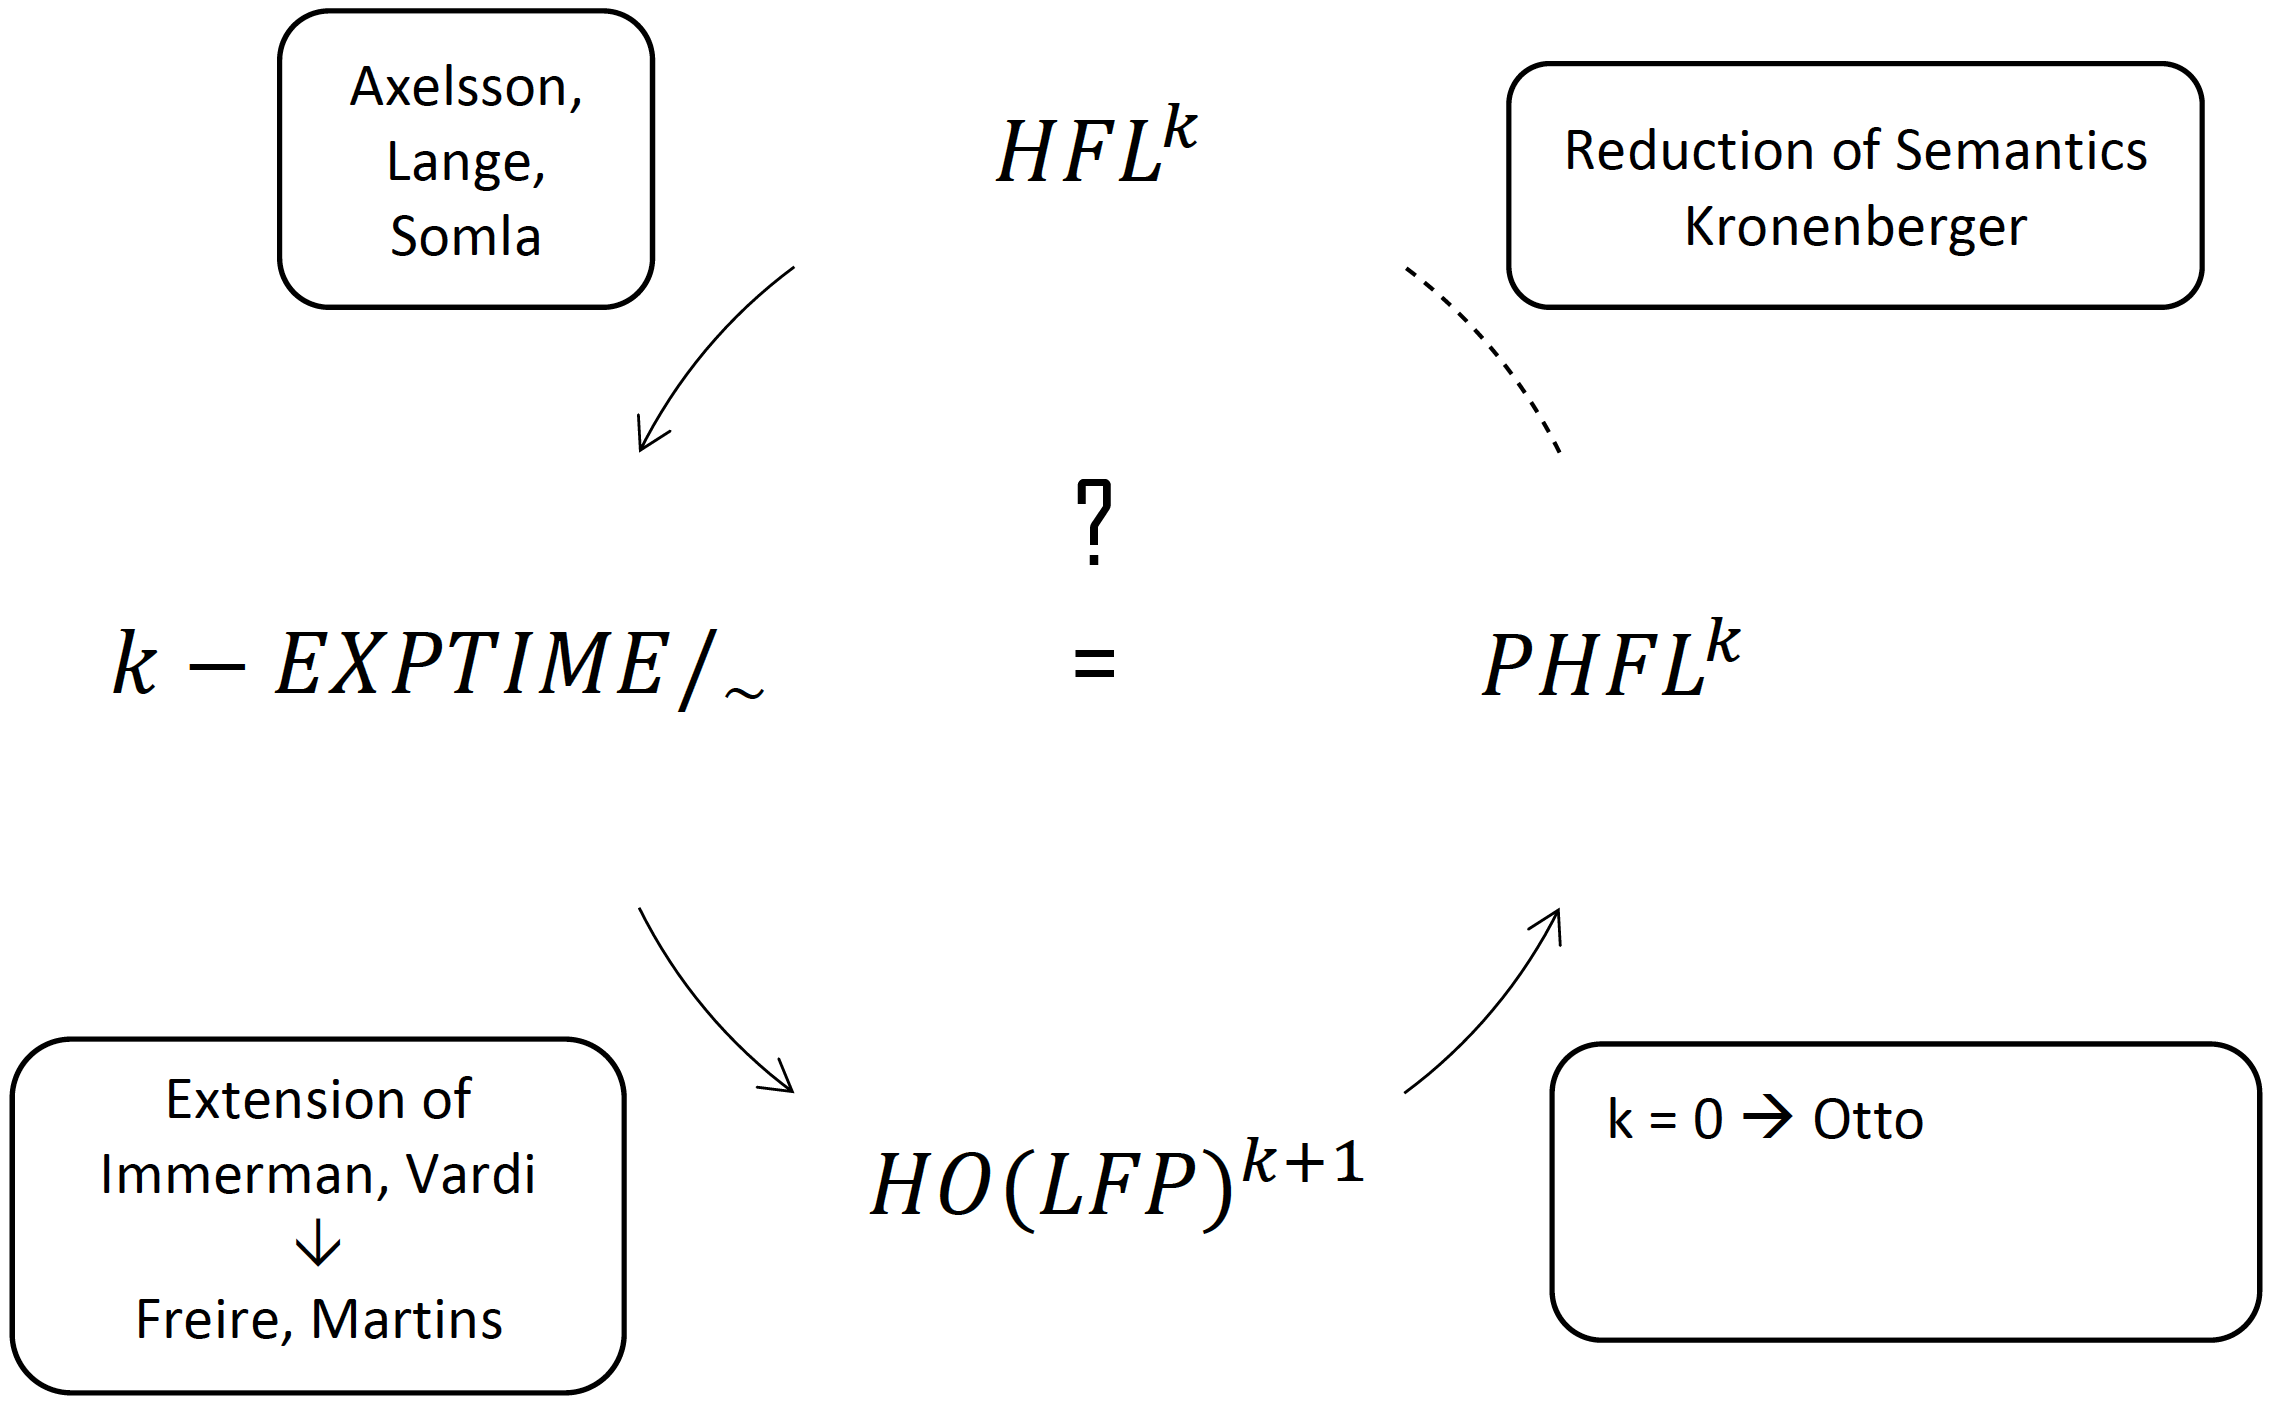
\includegraphics[width=0.9\textwidth]{phfl_7.png}}
  \only<9>{\hspace{-0.8cm}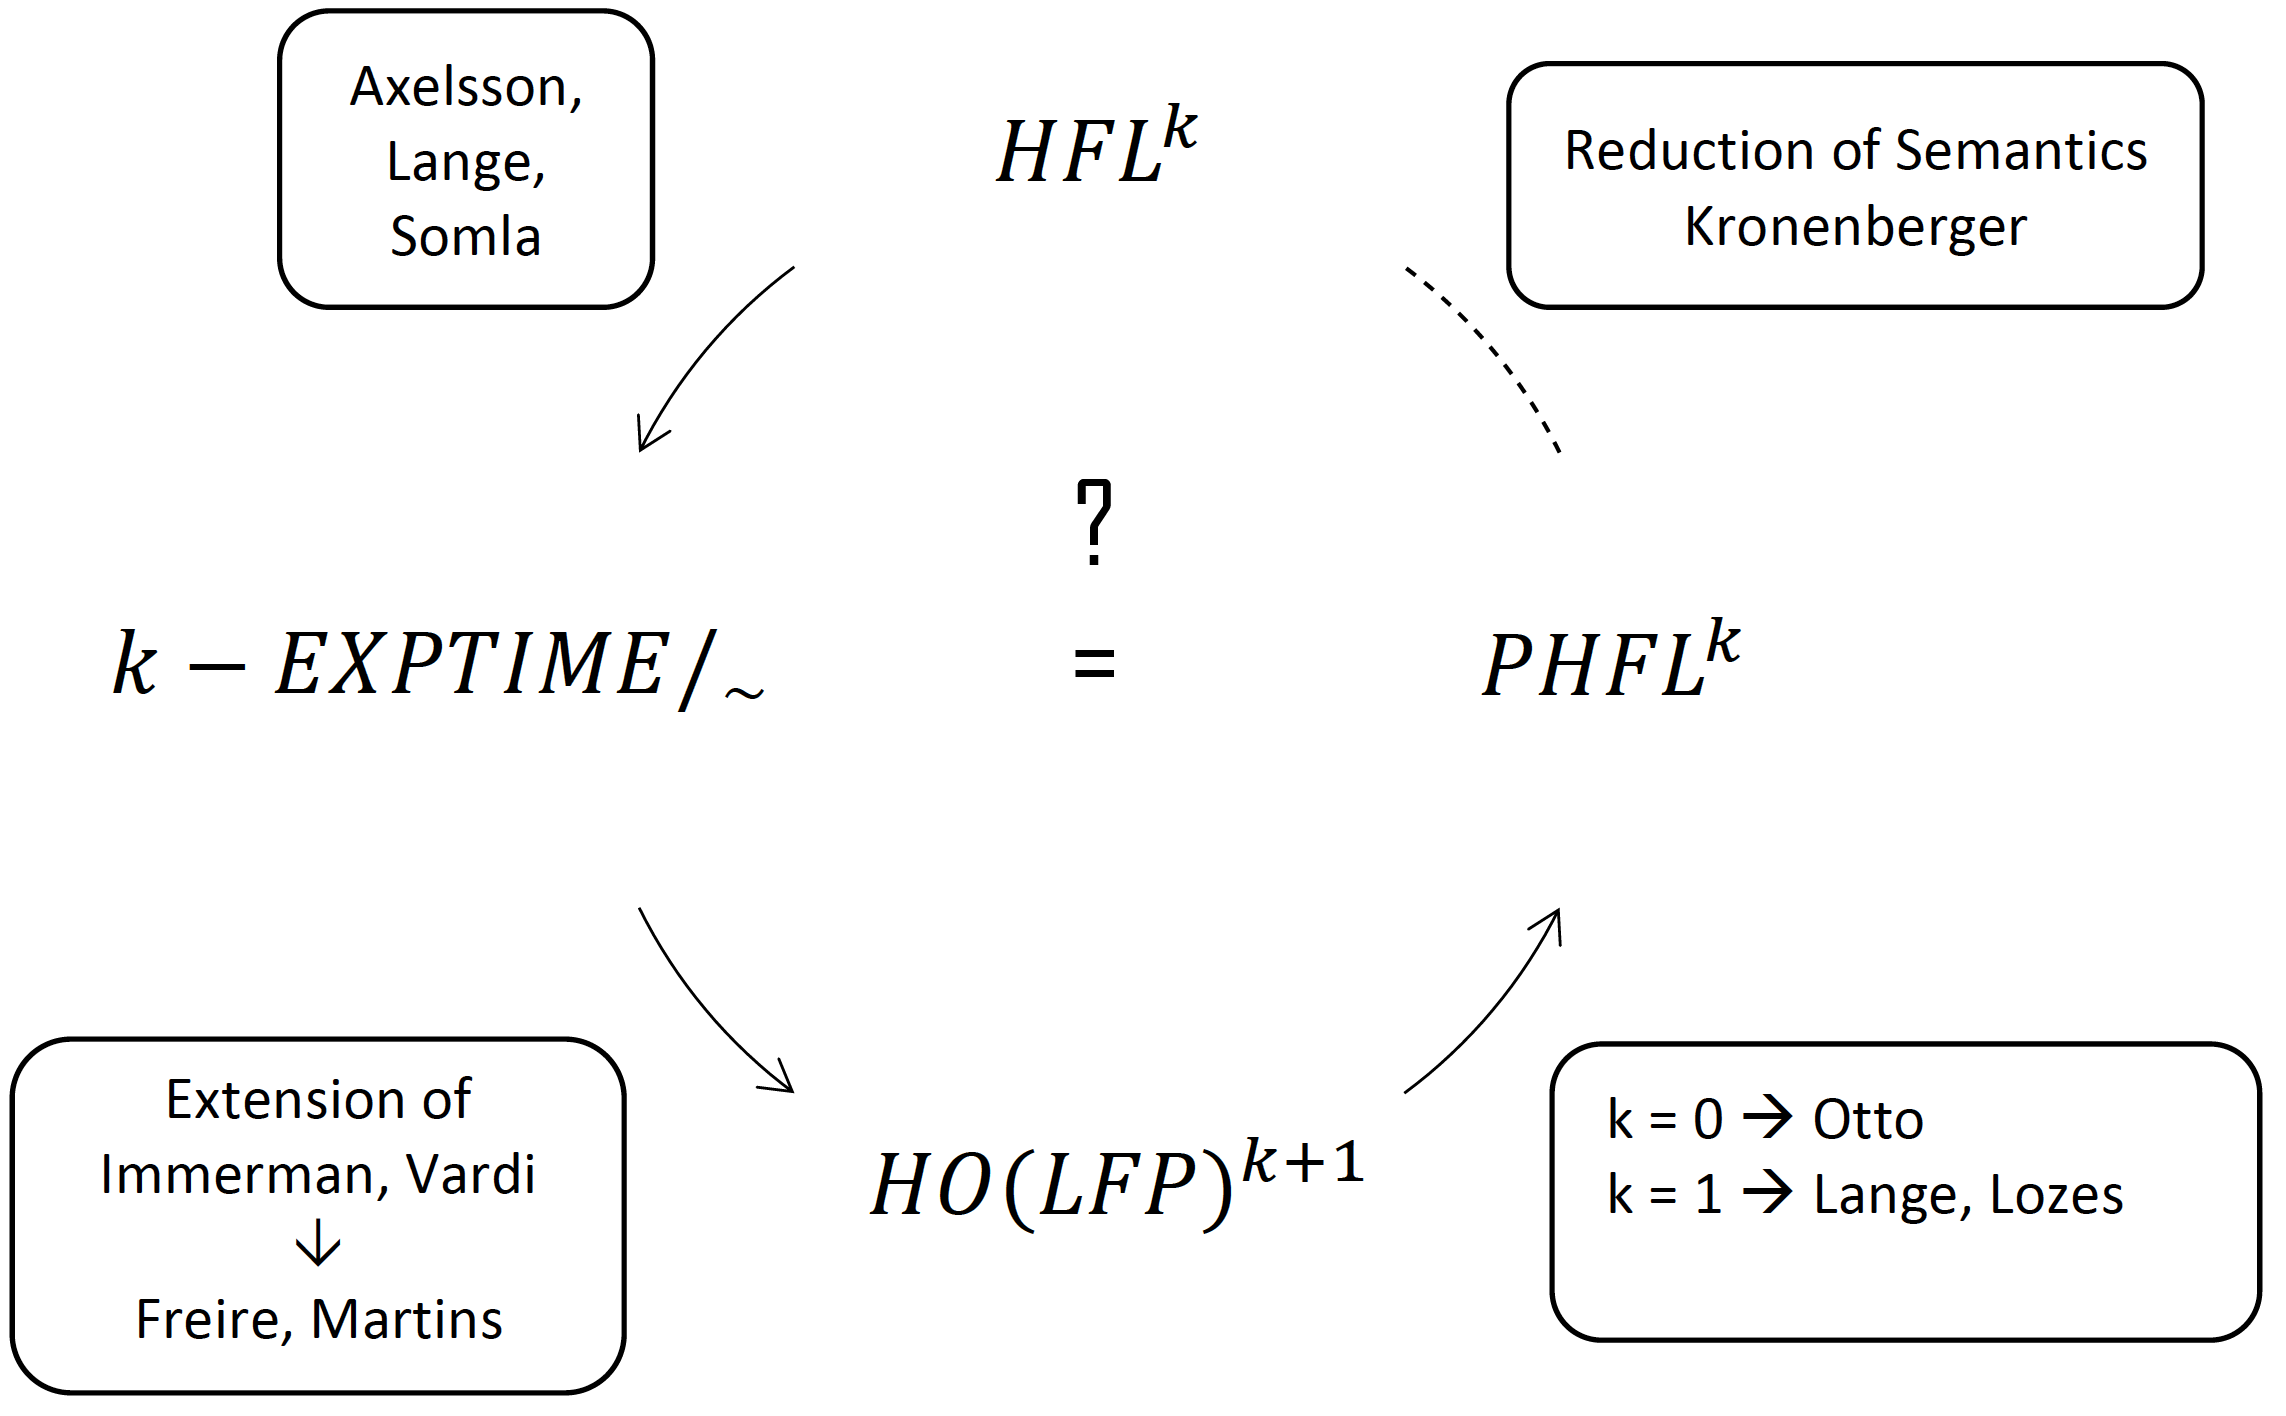
\includegraphics[width=0.9\textwidth]{phfl_8.png}}
  \only<10>{\hspace{-0.9cm}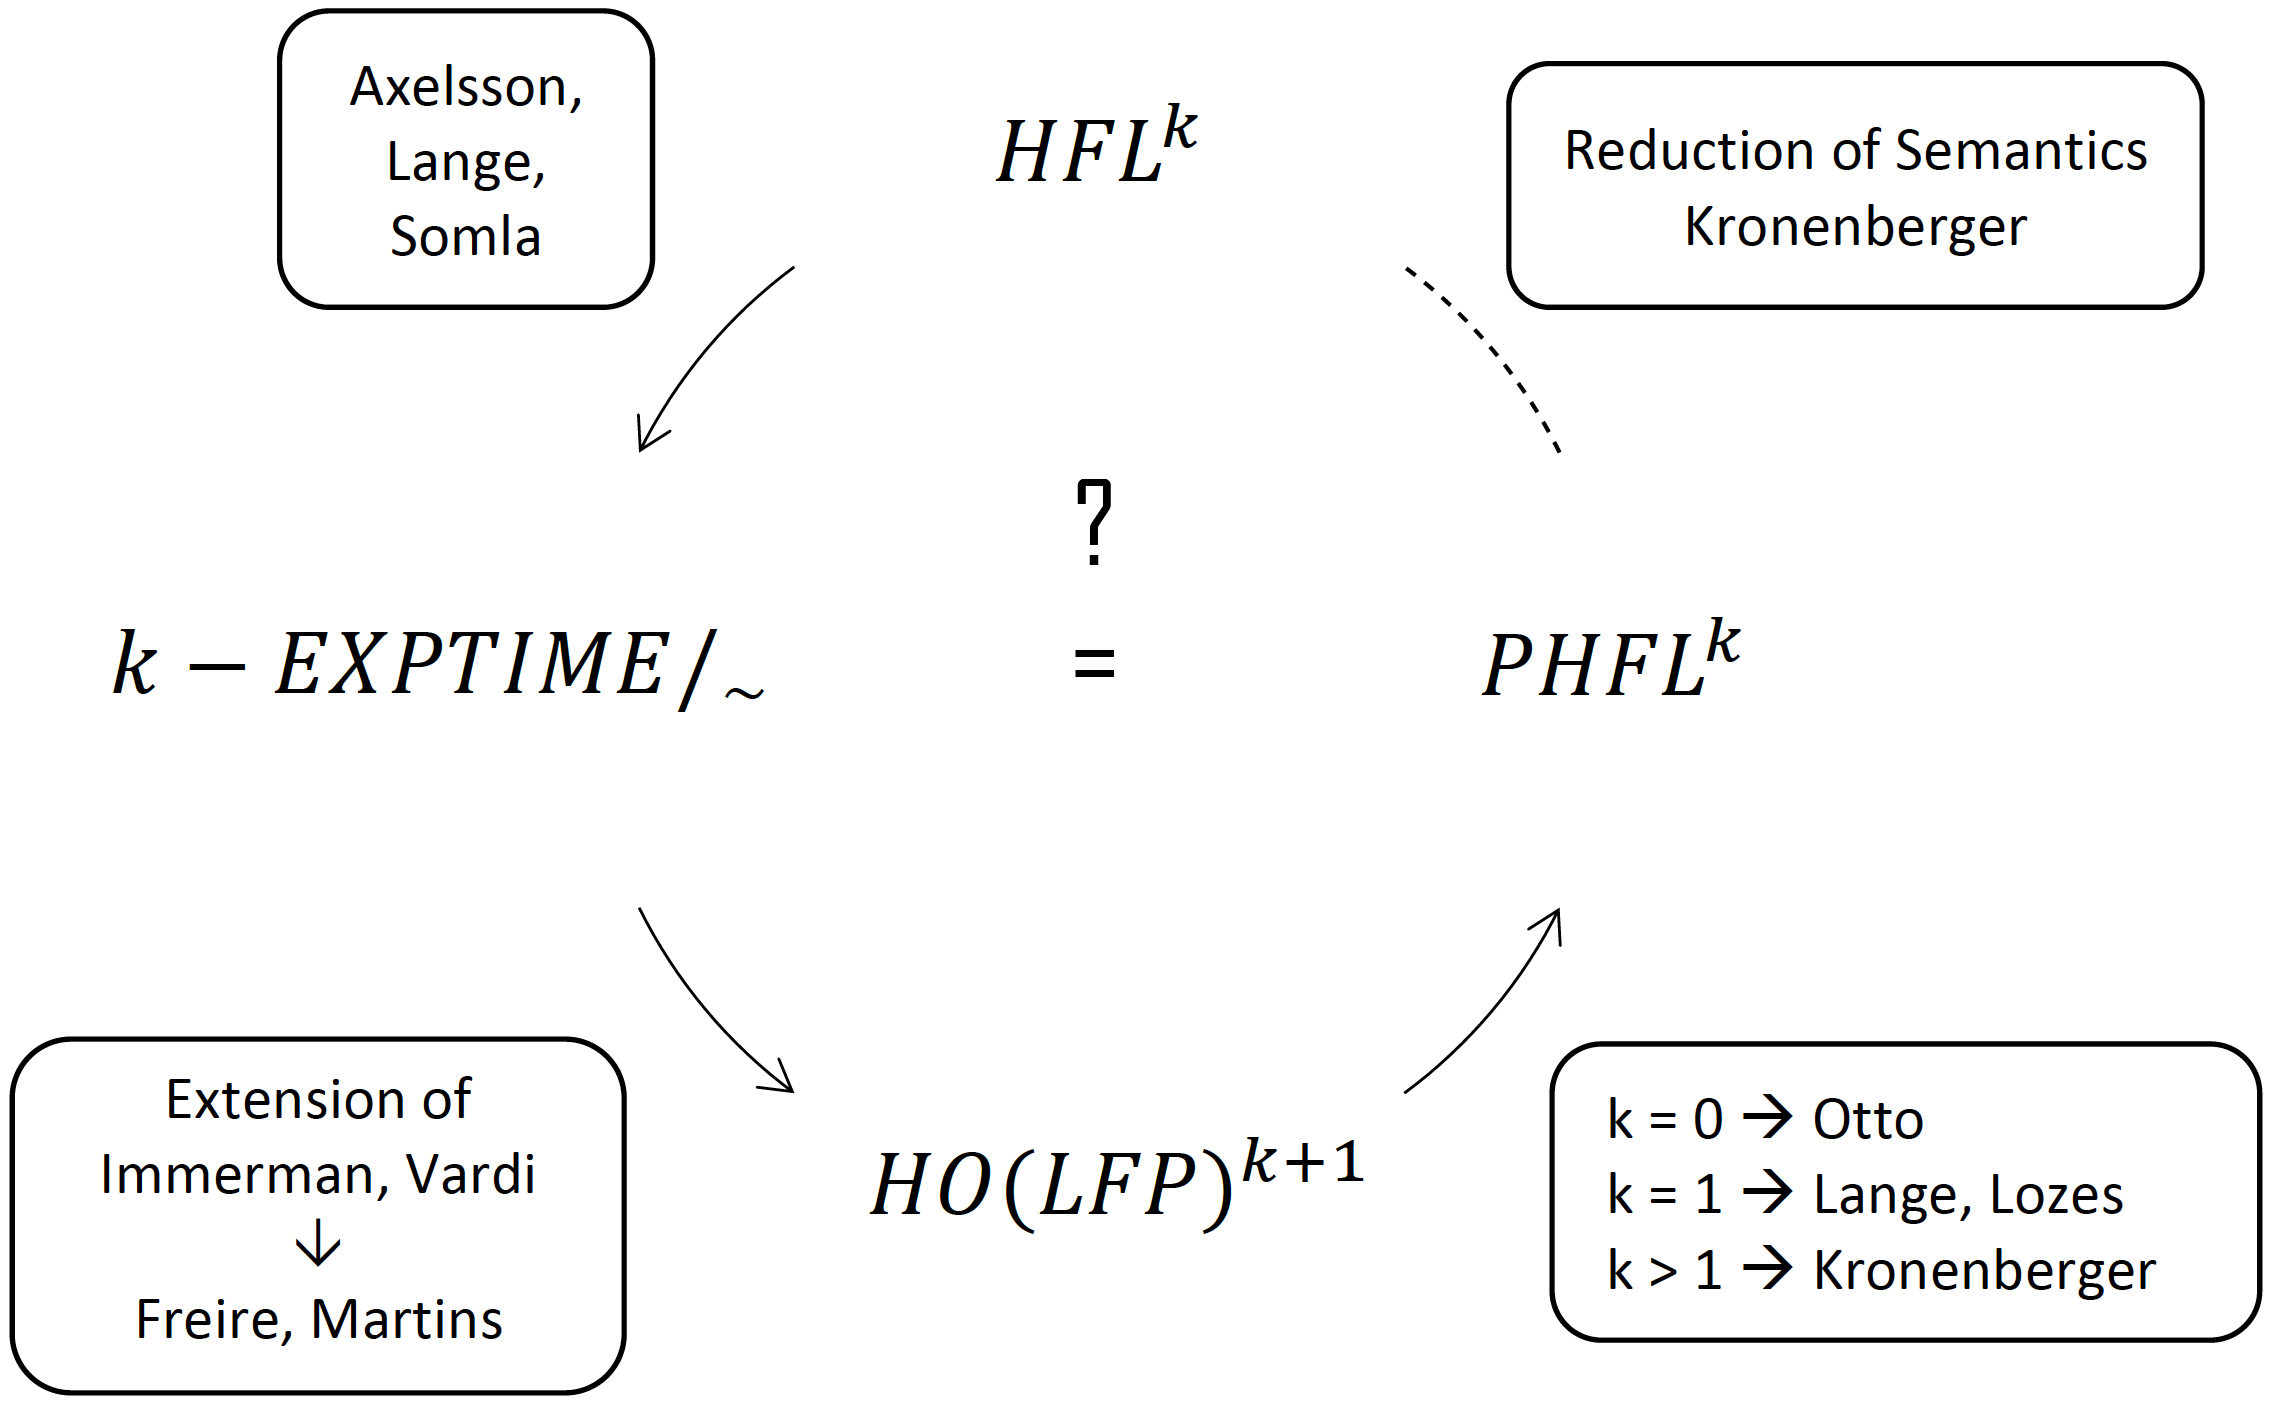
\includegraphics[width=0.9\textwidth]{phfl_9.png}}
  \only<11>{\hspace{-1.0cm}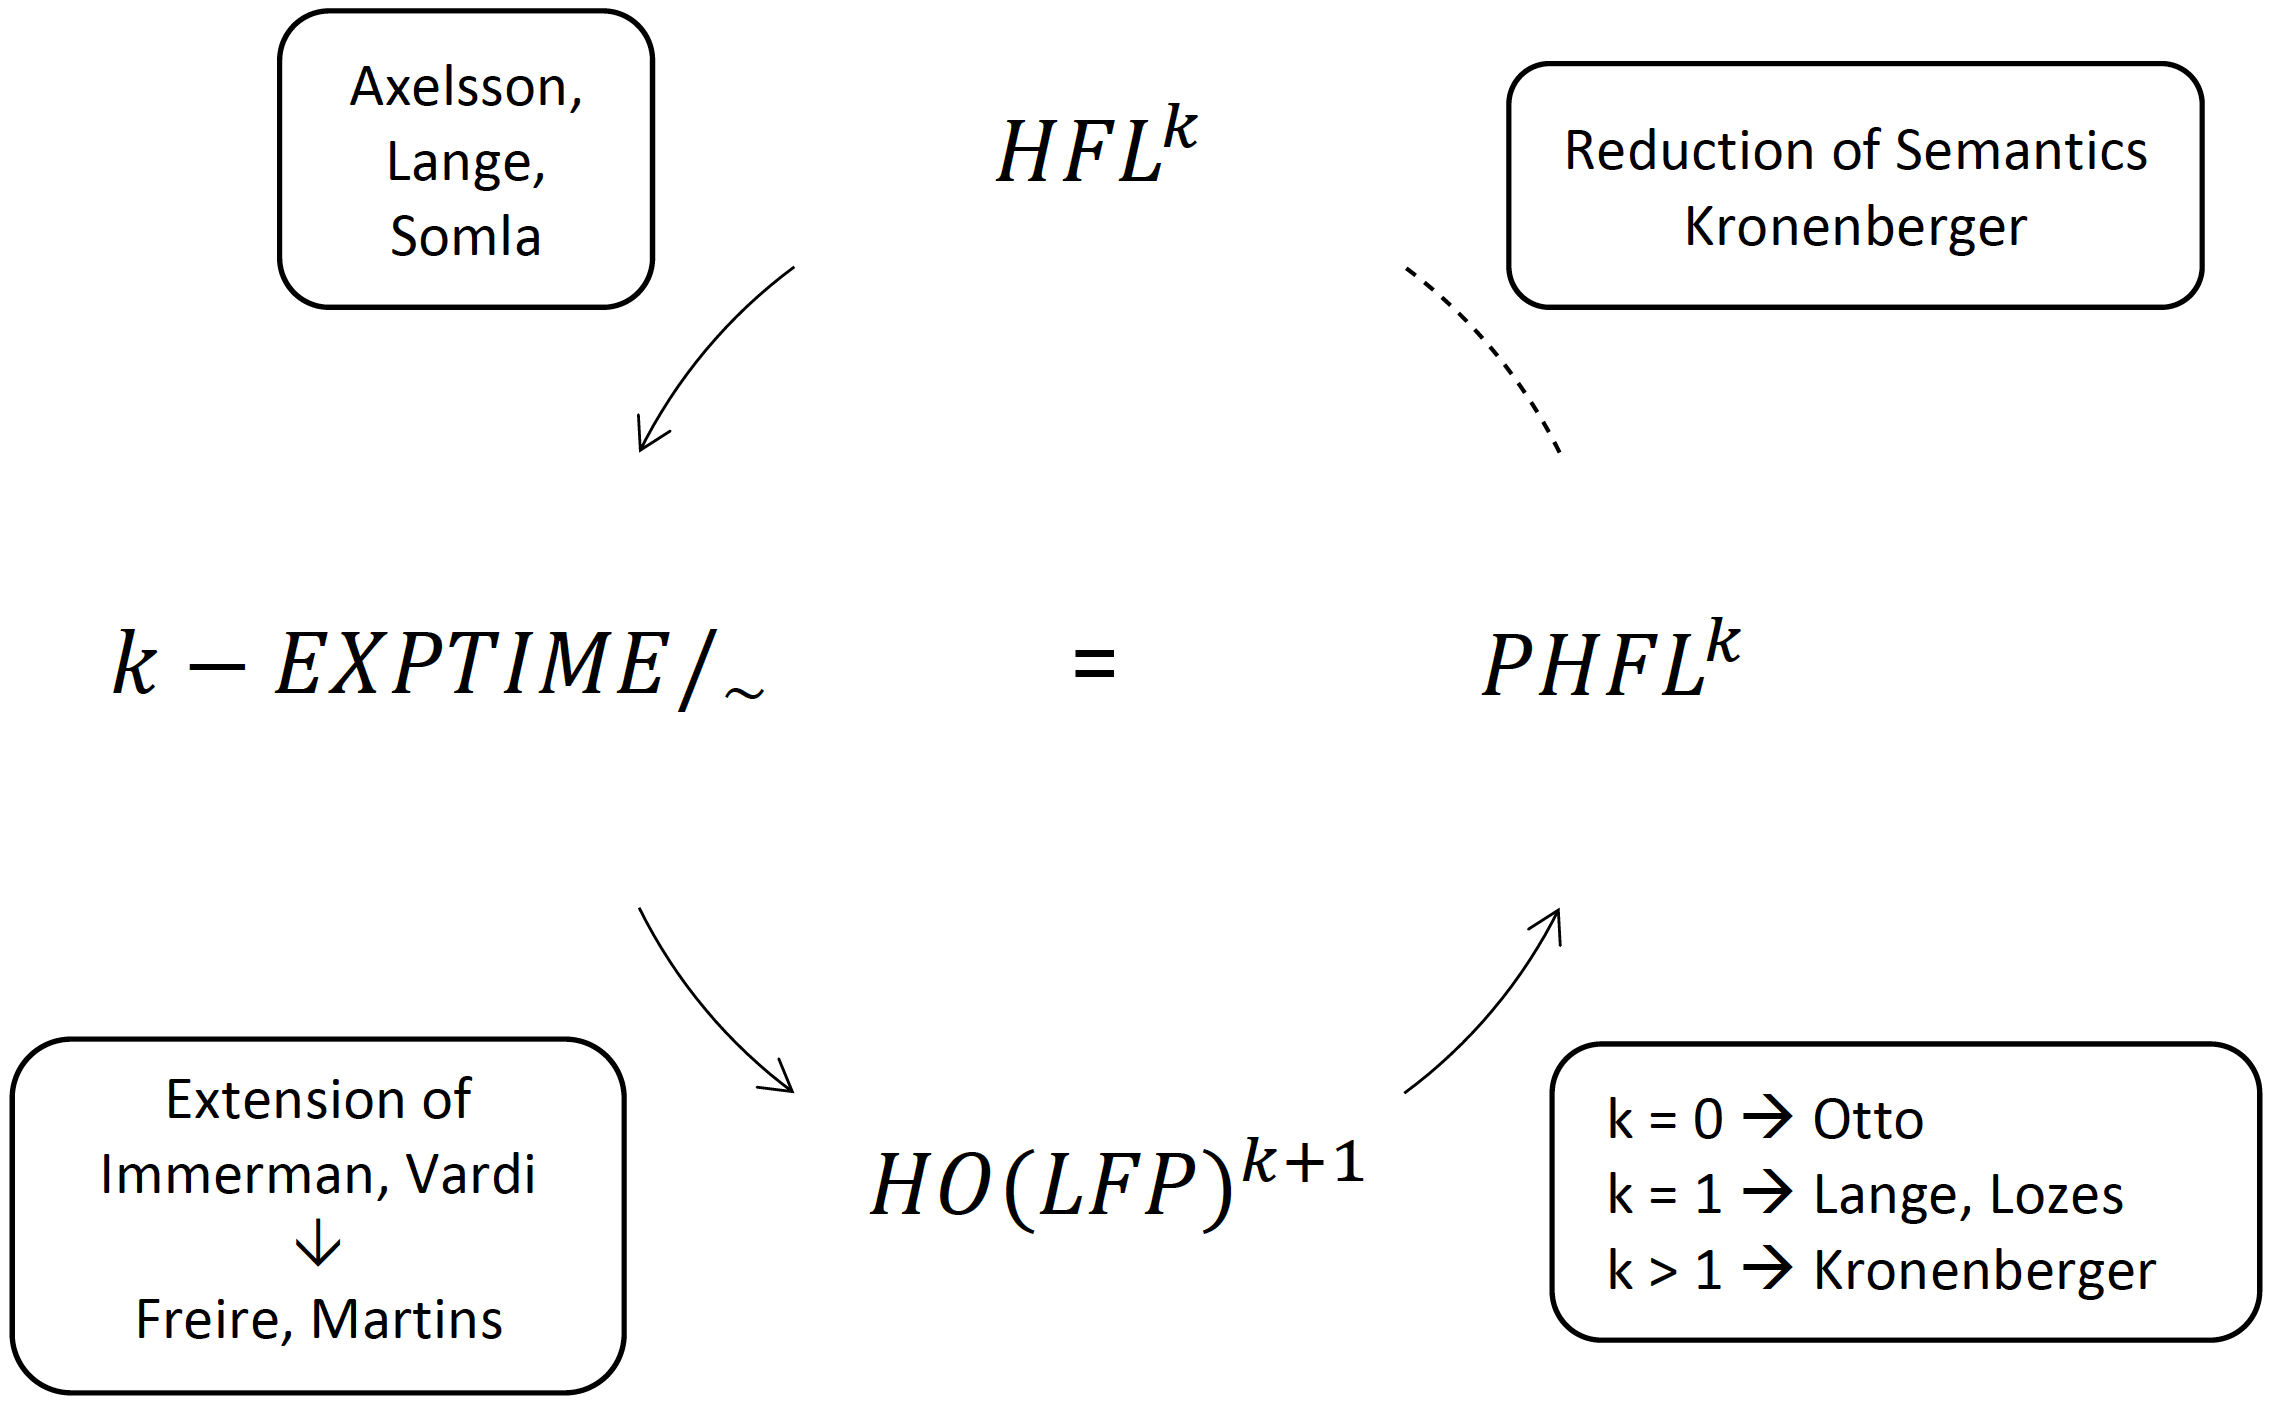
\includegraphics[width=0.9\textwidth]{phfl.png}}}
\end{figure}


\end{frame}
\begin{frame}

\begin{figure}[ht]
	\centering{
  \only<1>{\hspace{-0.1cm}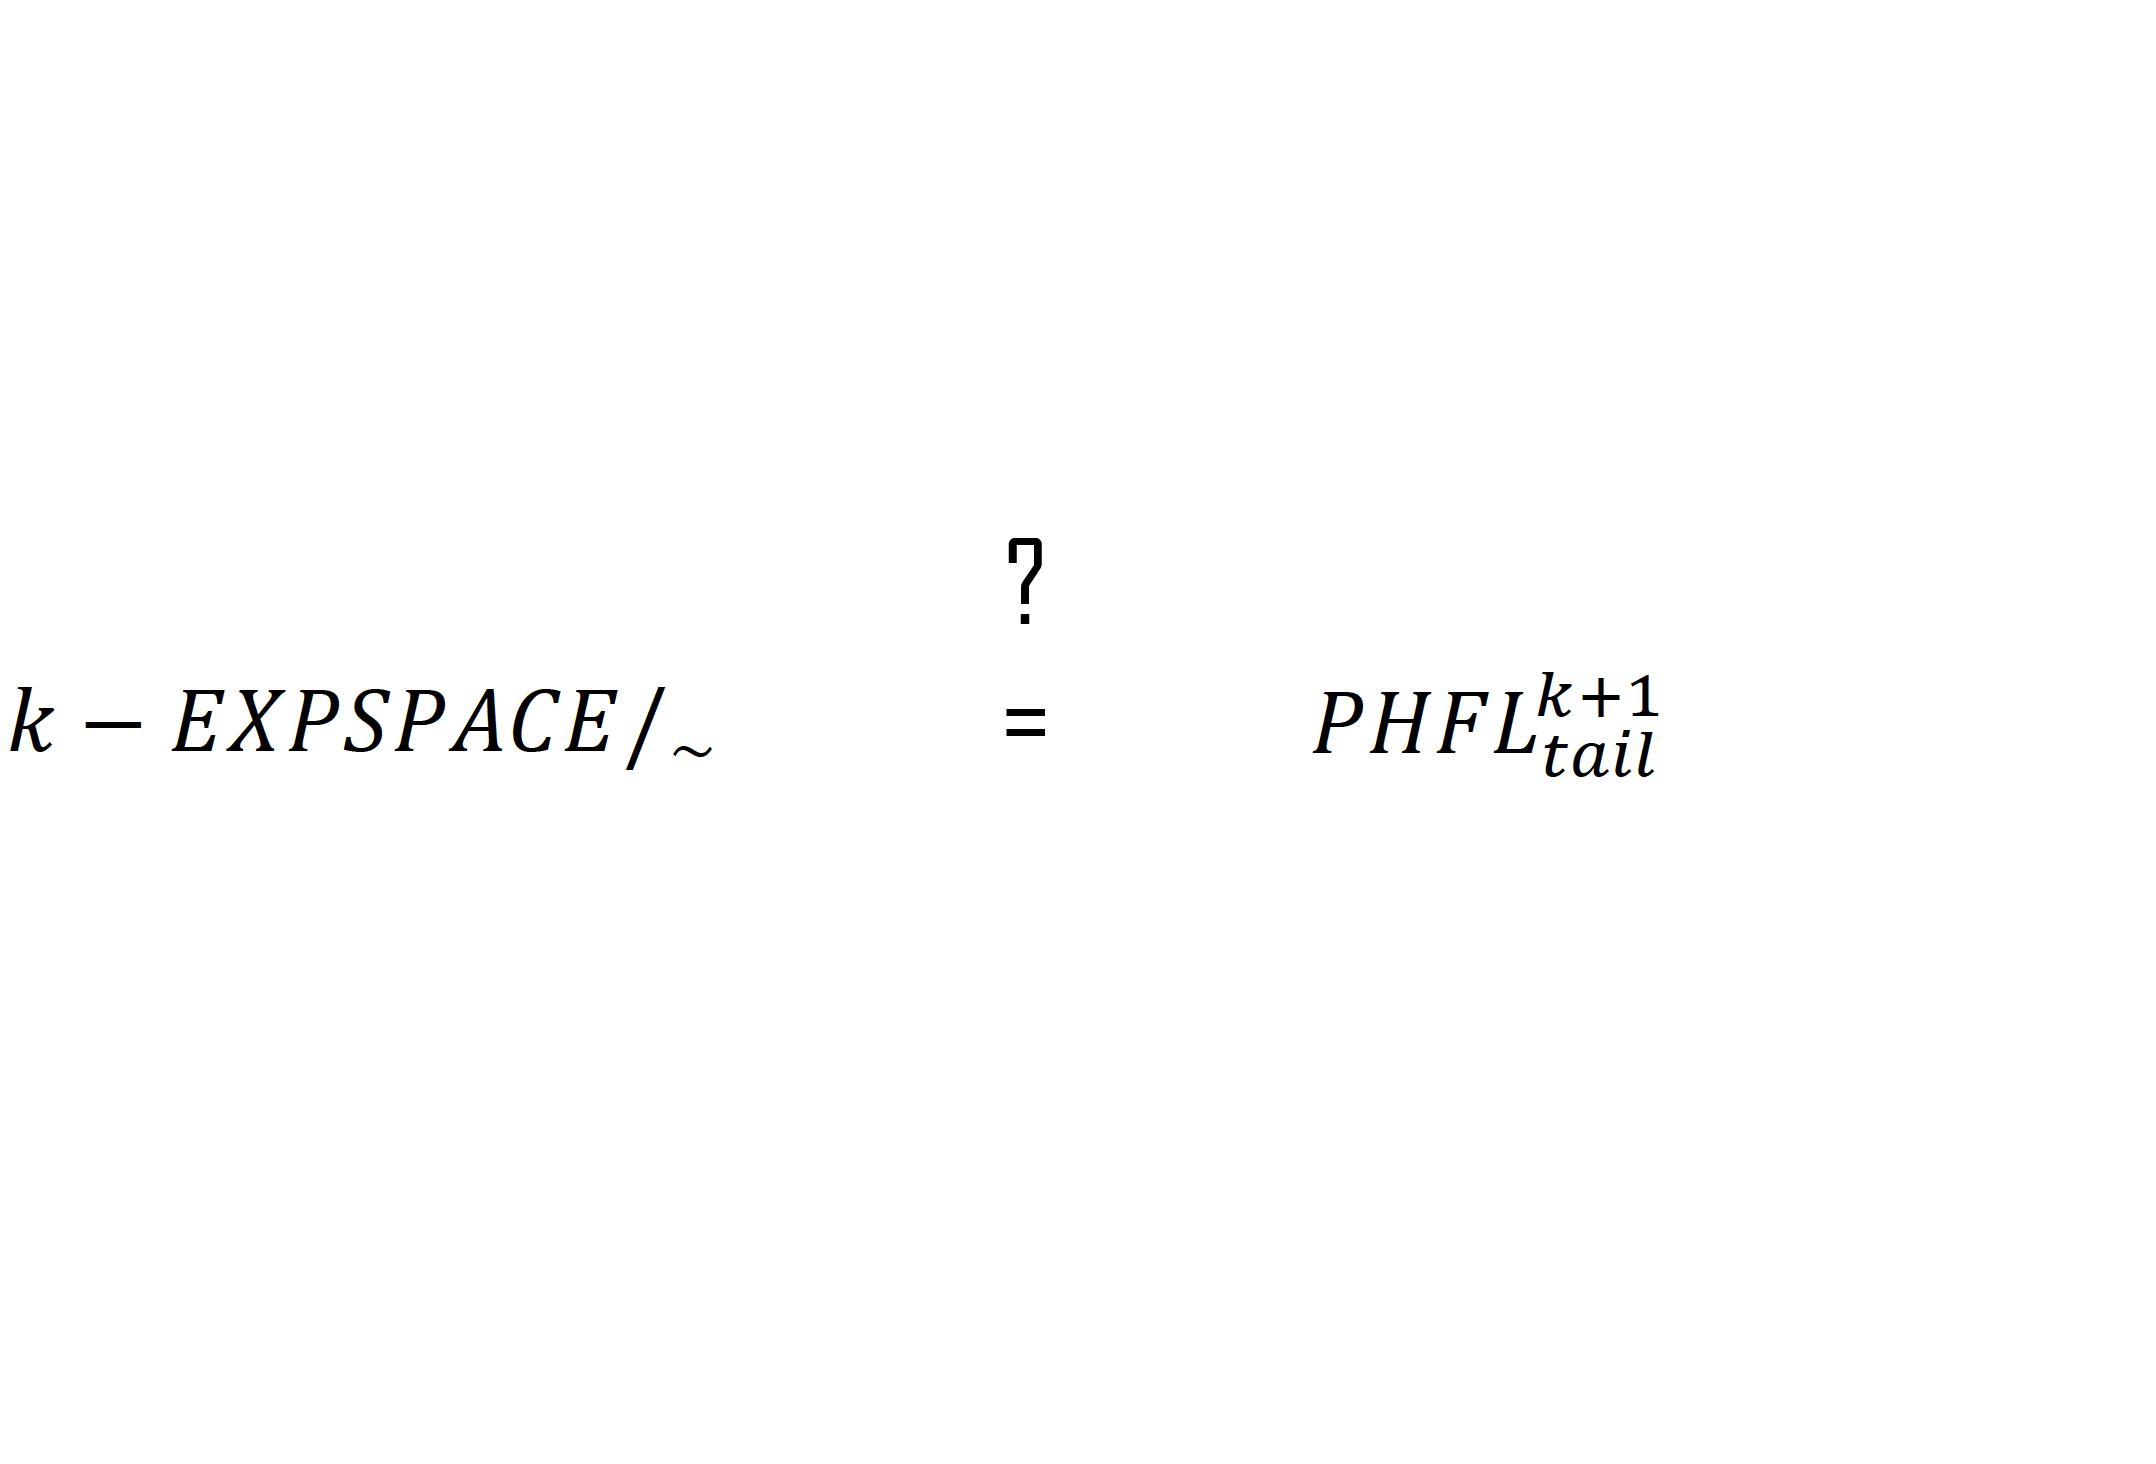
\includegraphics[width=0.9\textwidth]{phfl-tail_0.png}}
  \only<2>{\hspace{-0.1cm}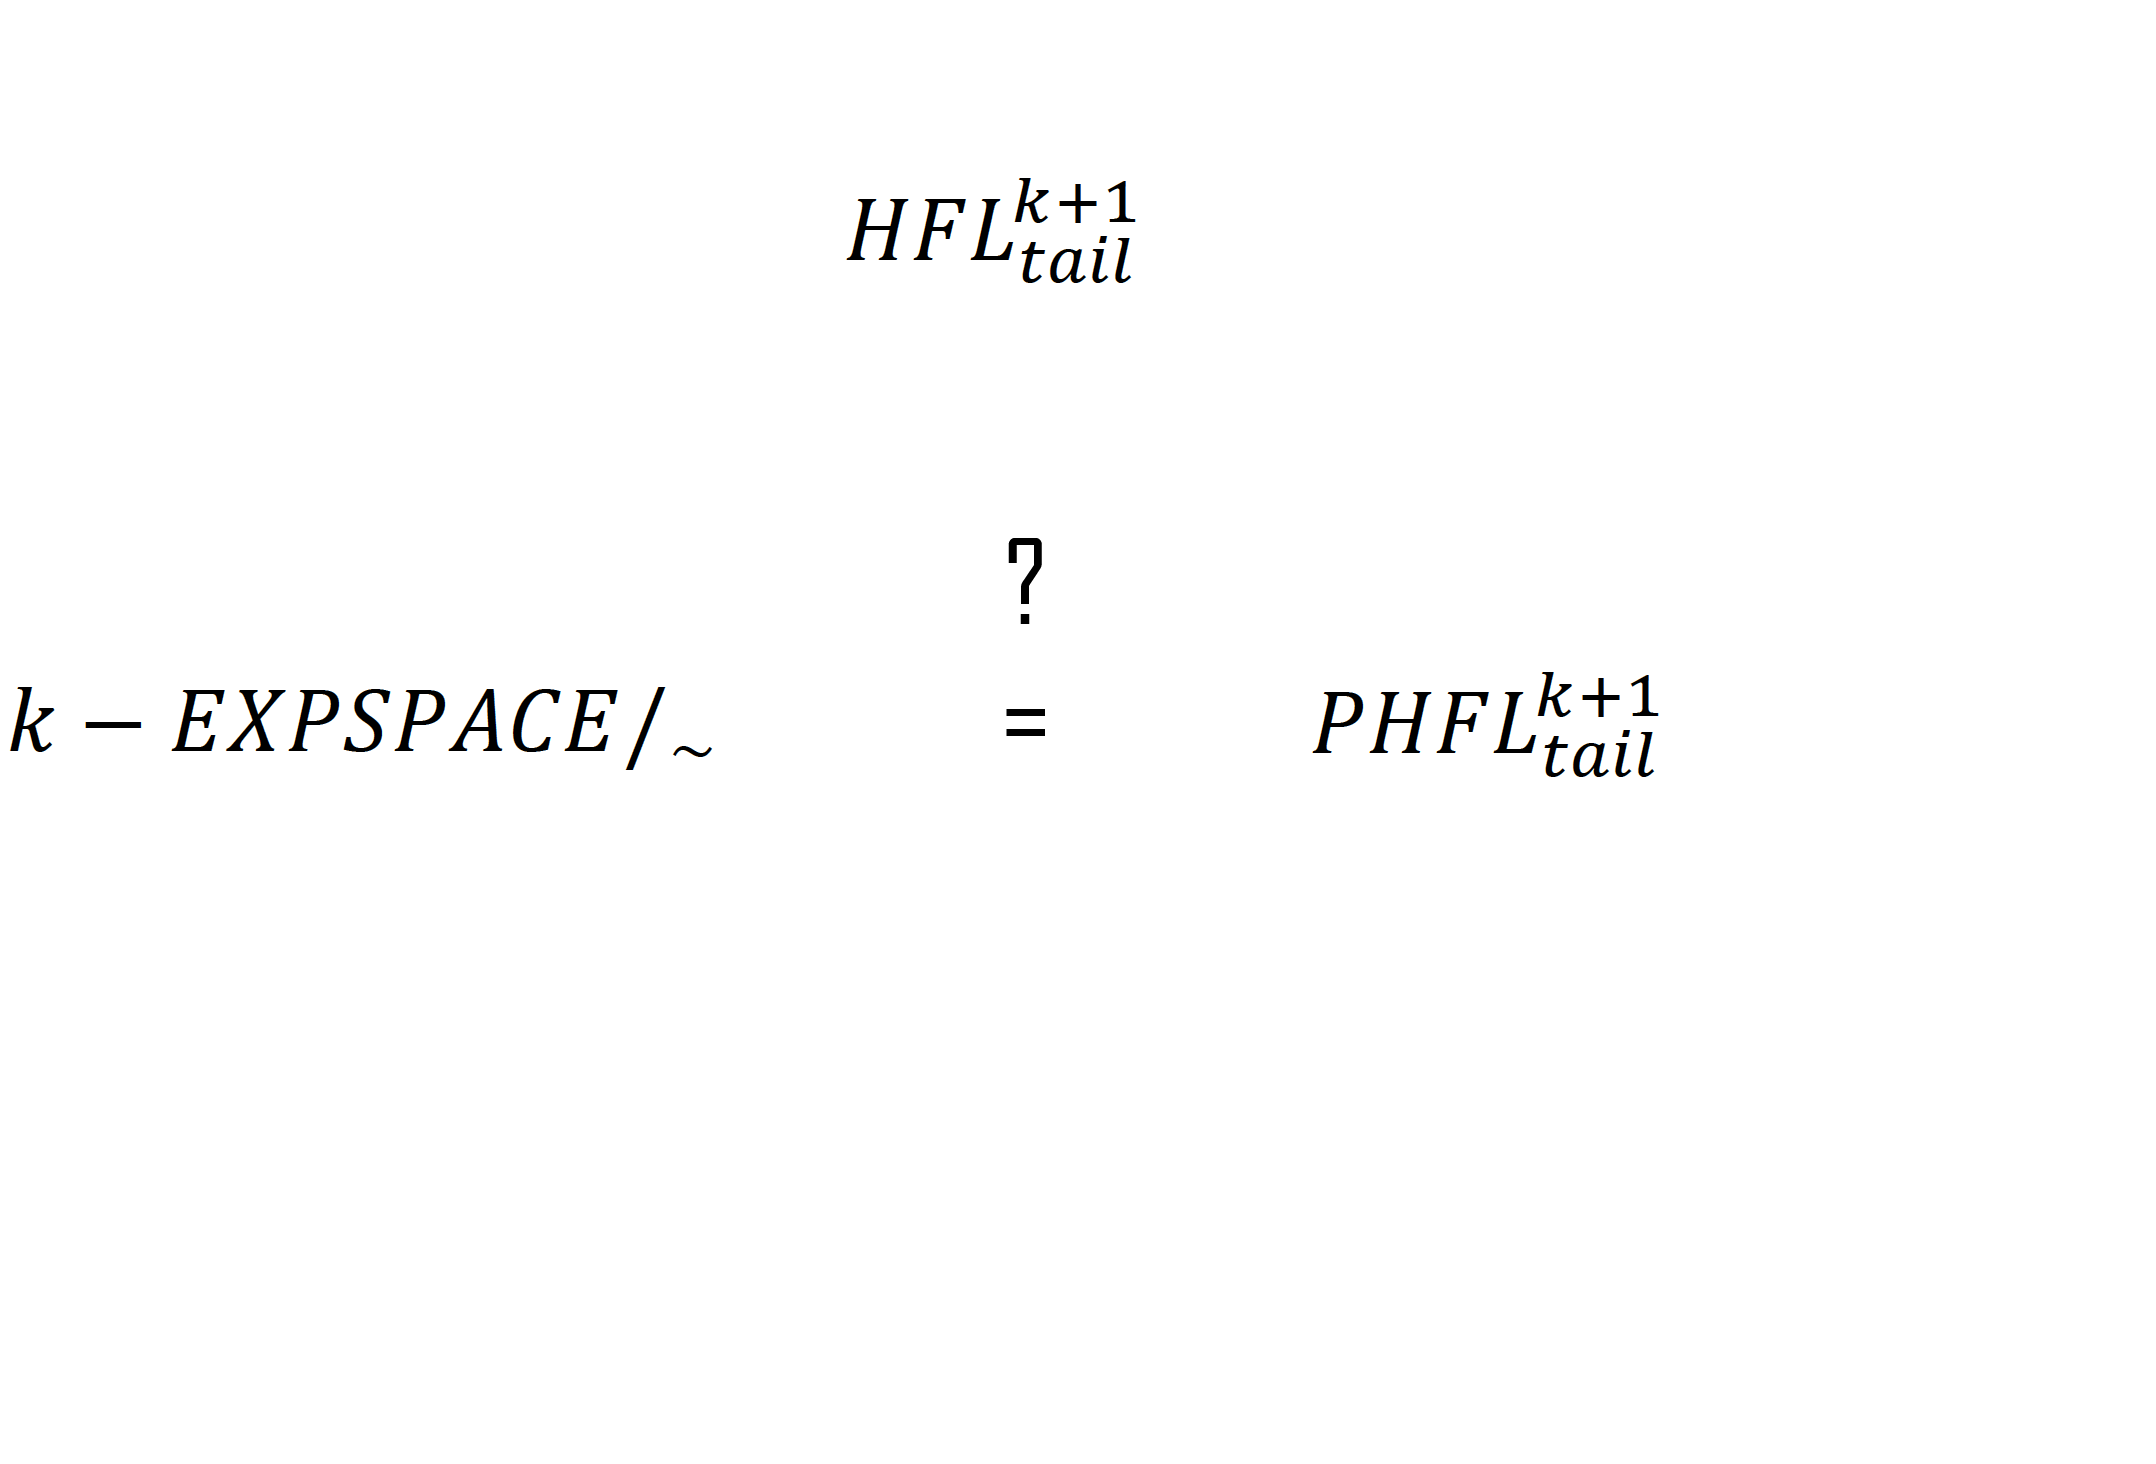
\includegraphics[width=0.9\textwidth]{phfl-tail_1.png}}
  \only<3>{\hspace{-0.2cm}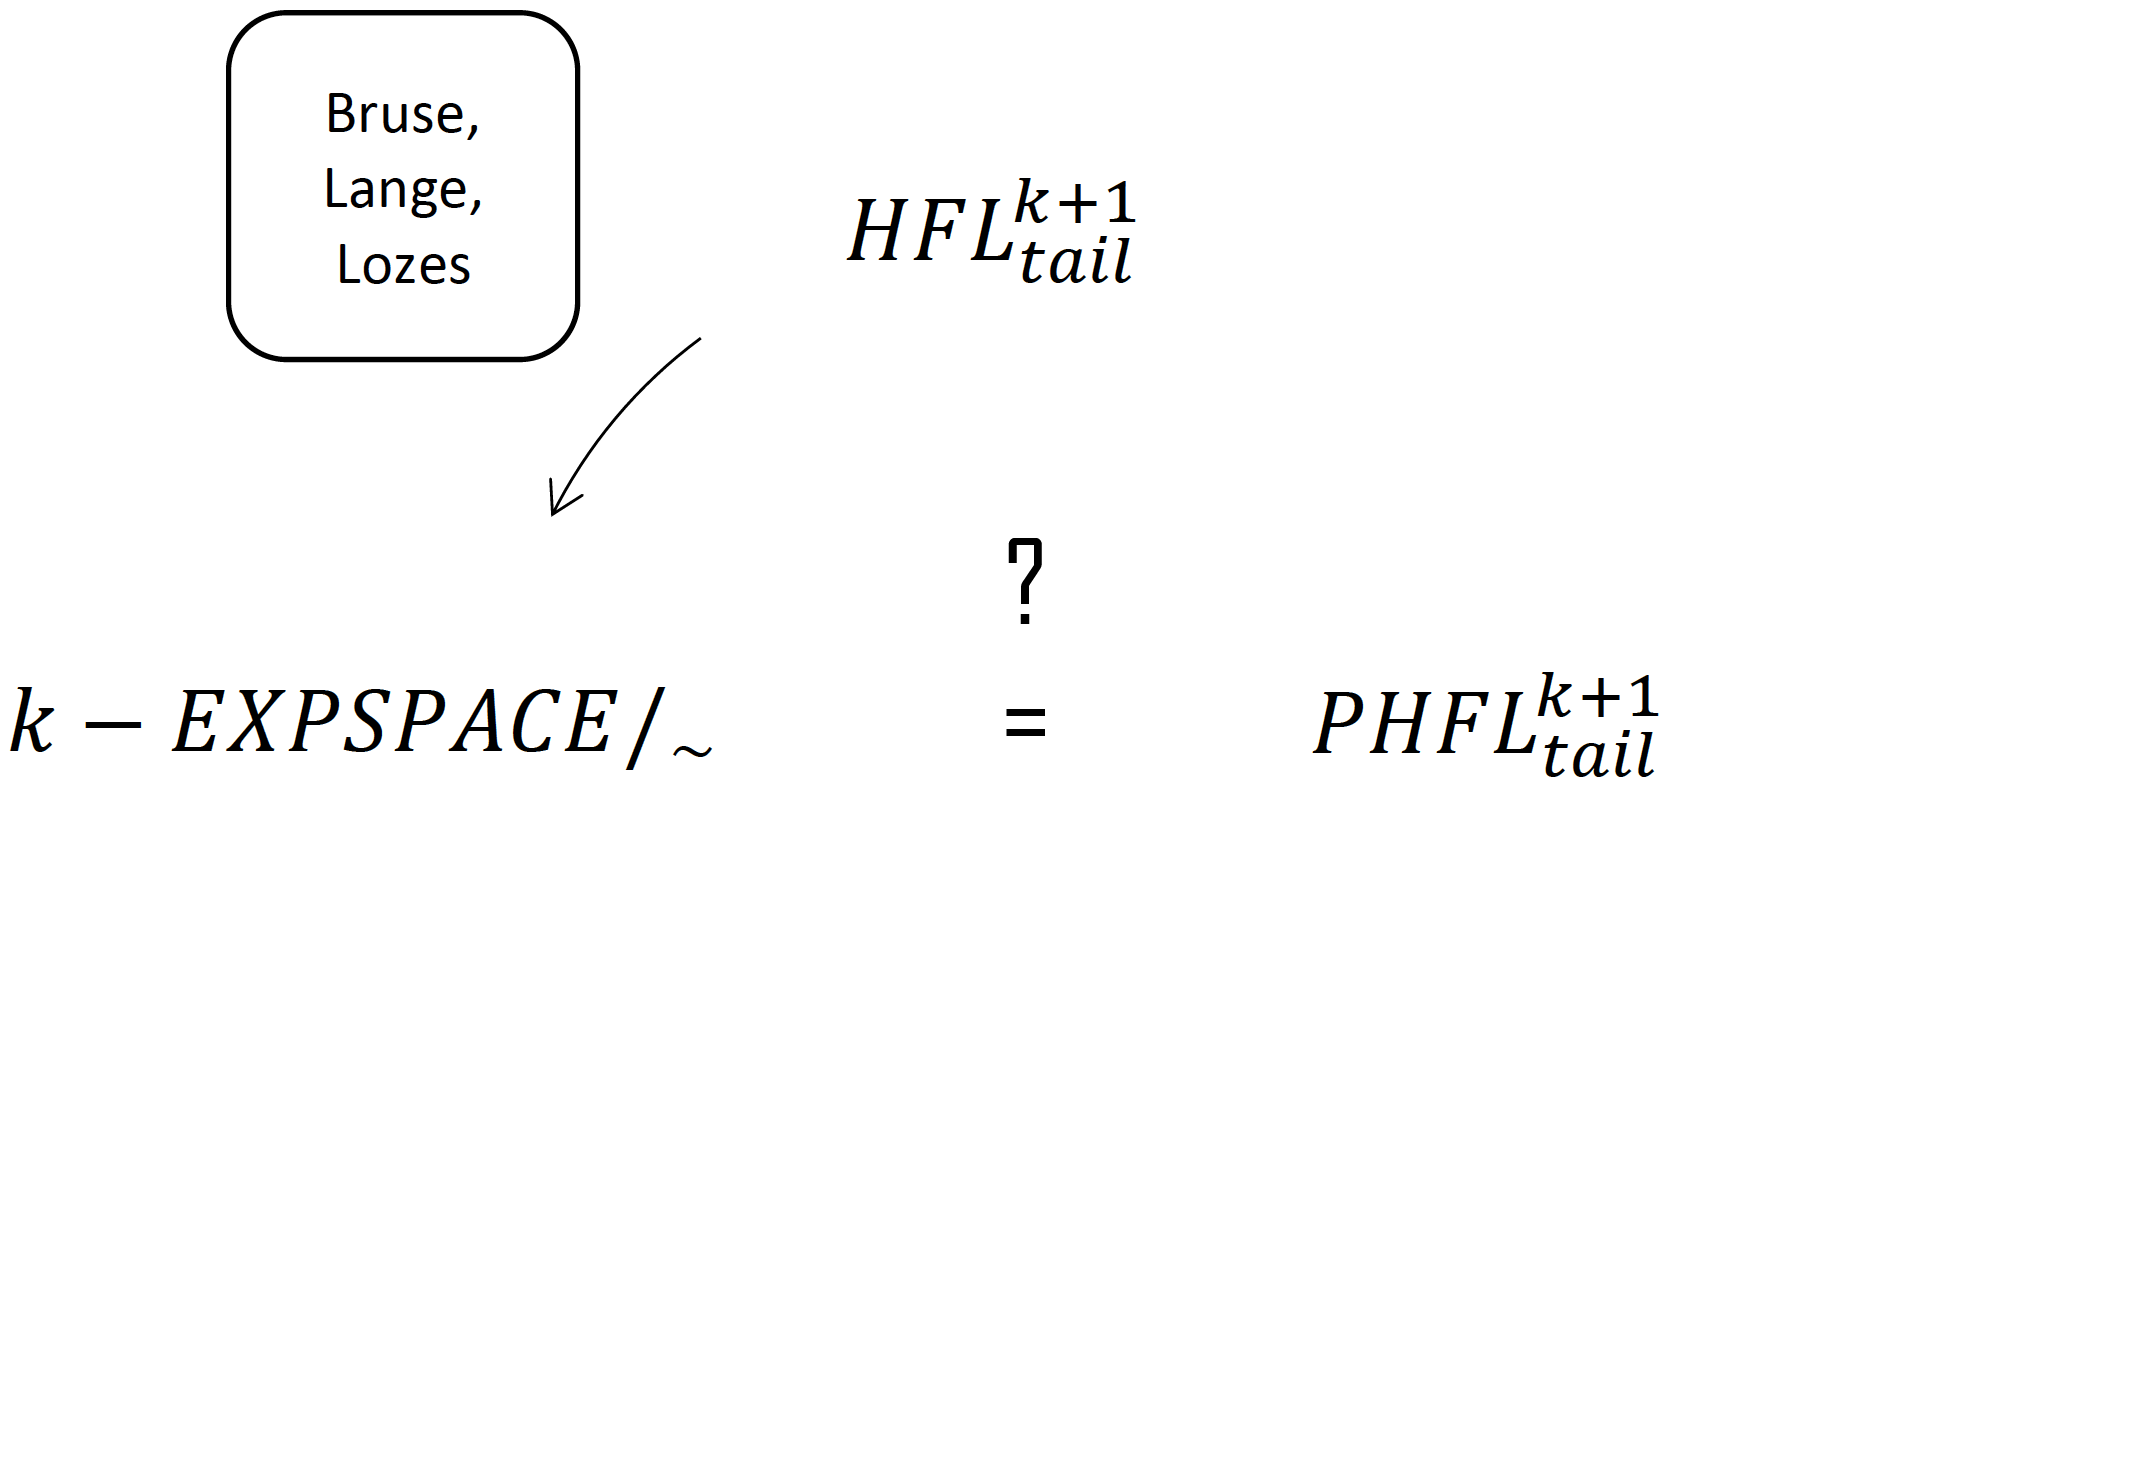
\includegraphics[width=0.9\textwidth]{phfl-tail_2.png}}
  \only<4>{\hspace{-0.3cm}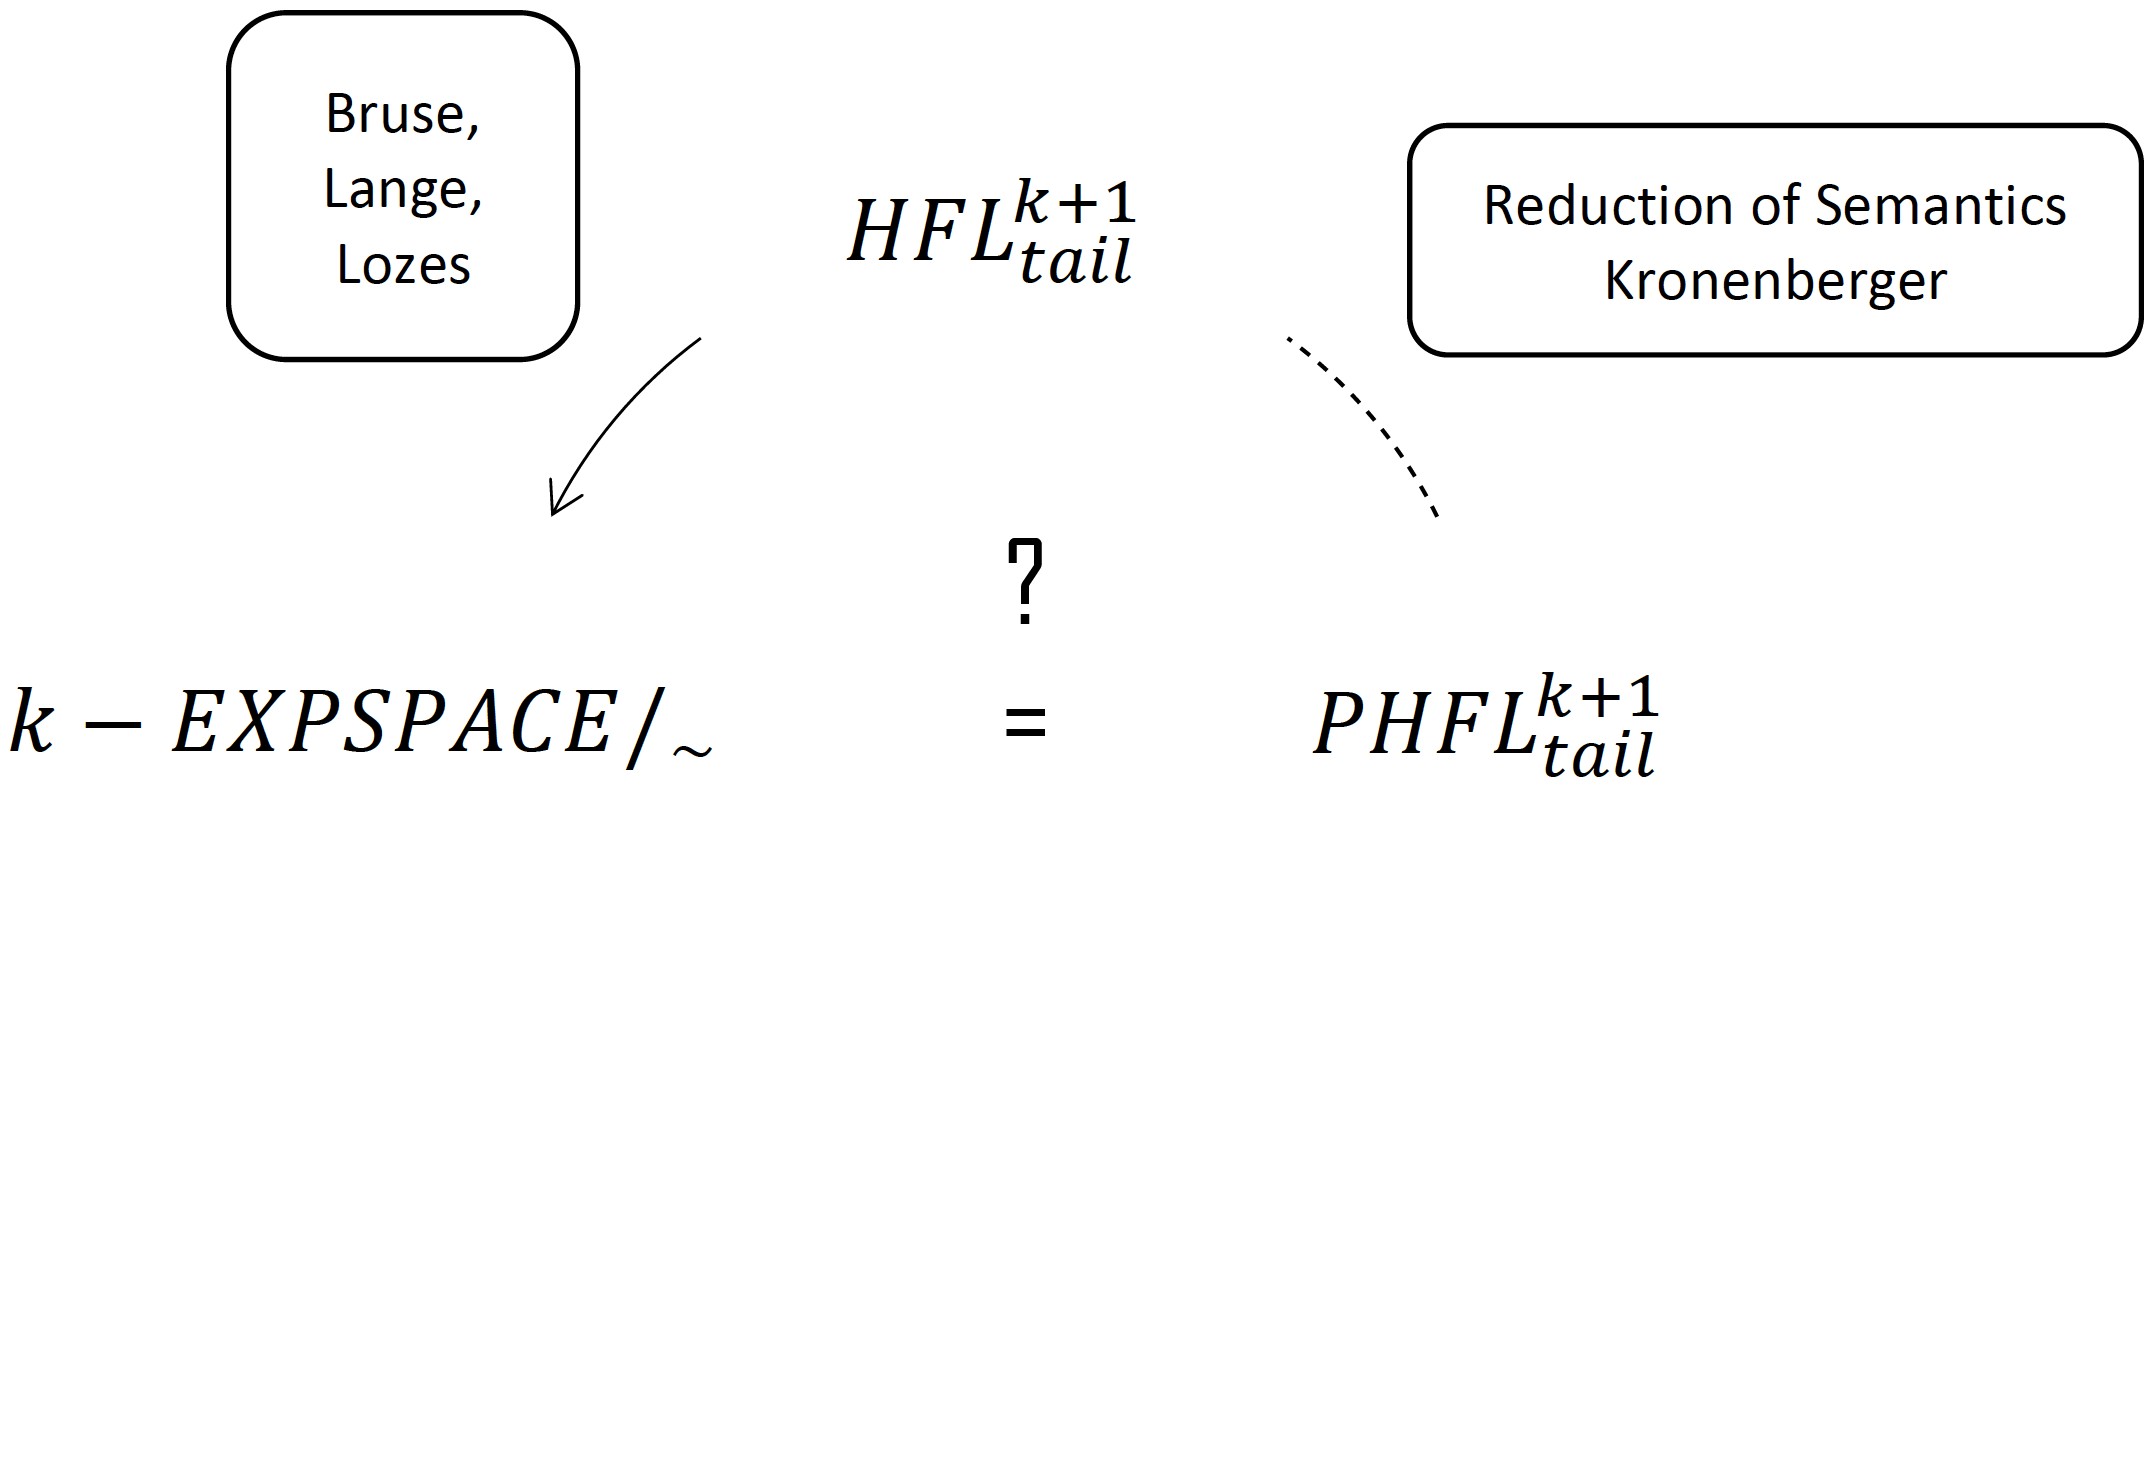
\includegraphics[width=0.9\textwidth]{phfl-tail_3.png}}
  \only<5>{\hspace{-0.4cm}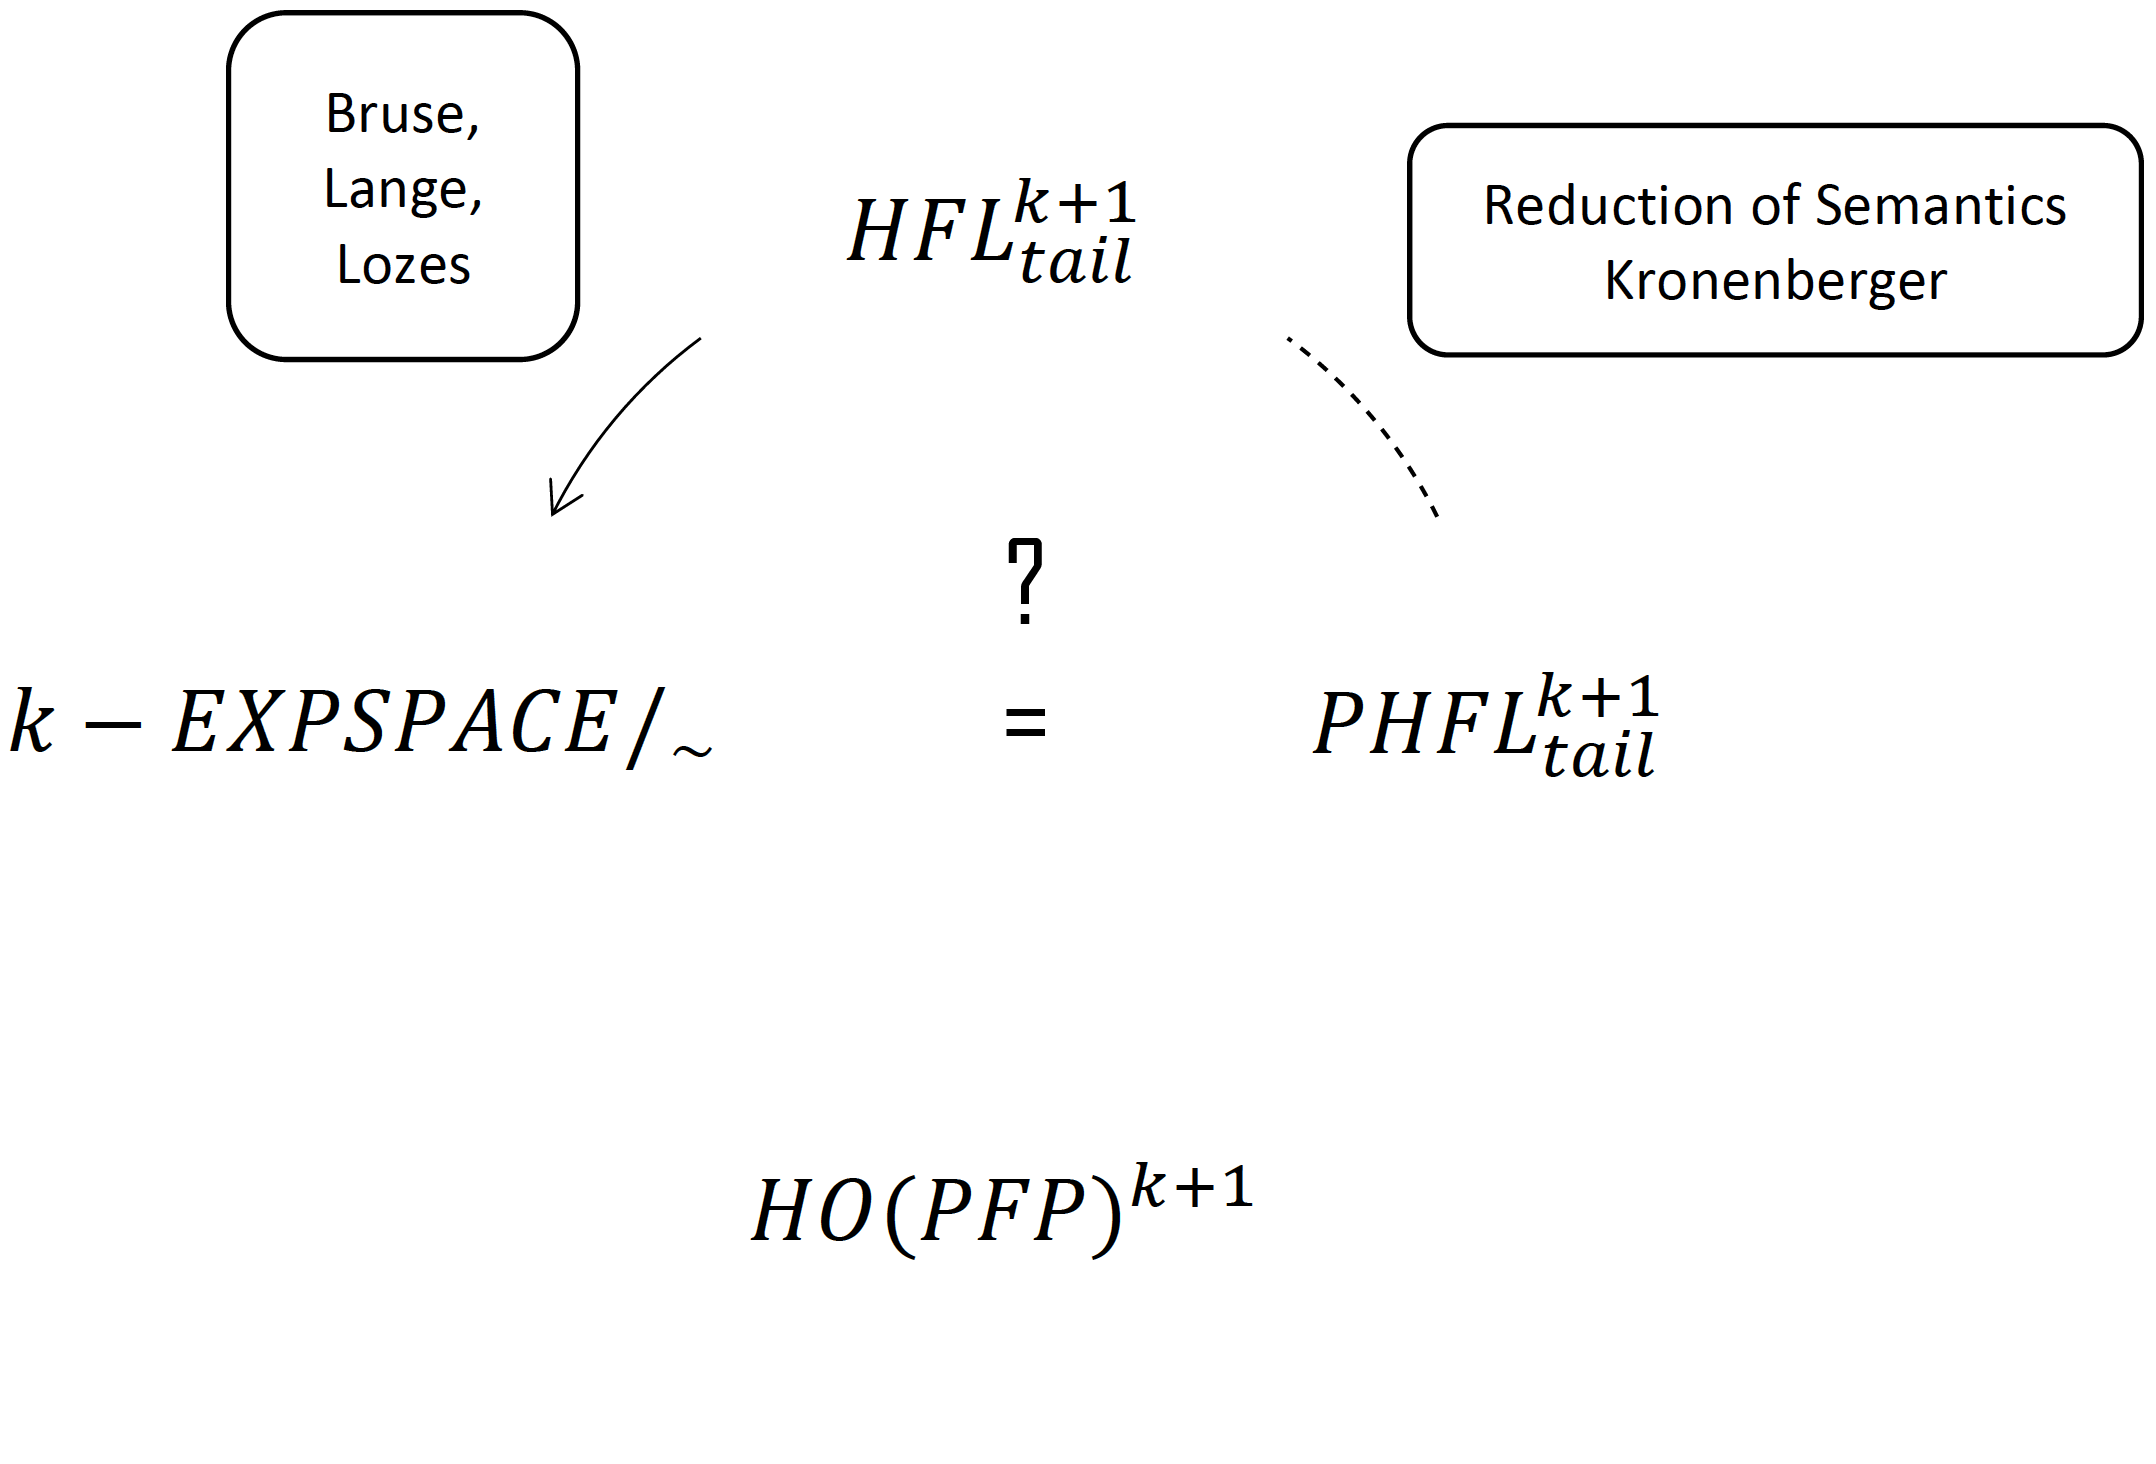
\includegraphics[width=0.9\textwidth]{phfl-tail_4.png}}
  \only<6>{\hspace{-0.5cm}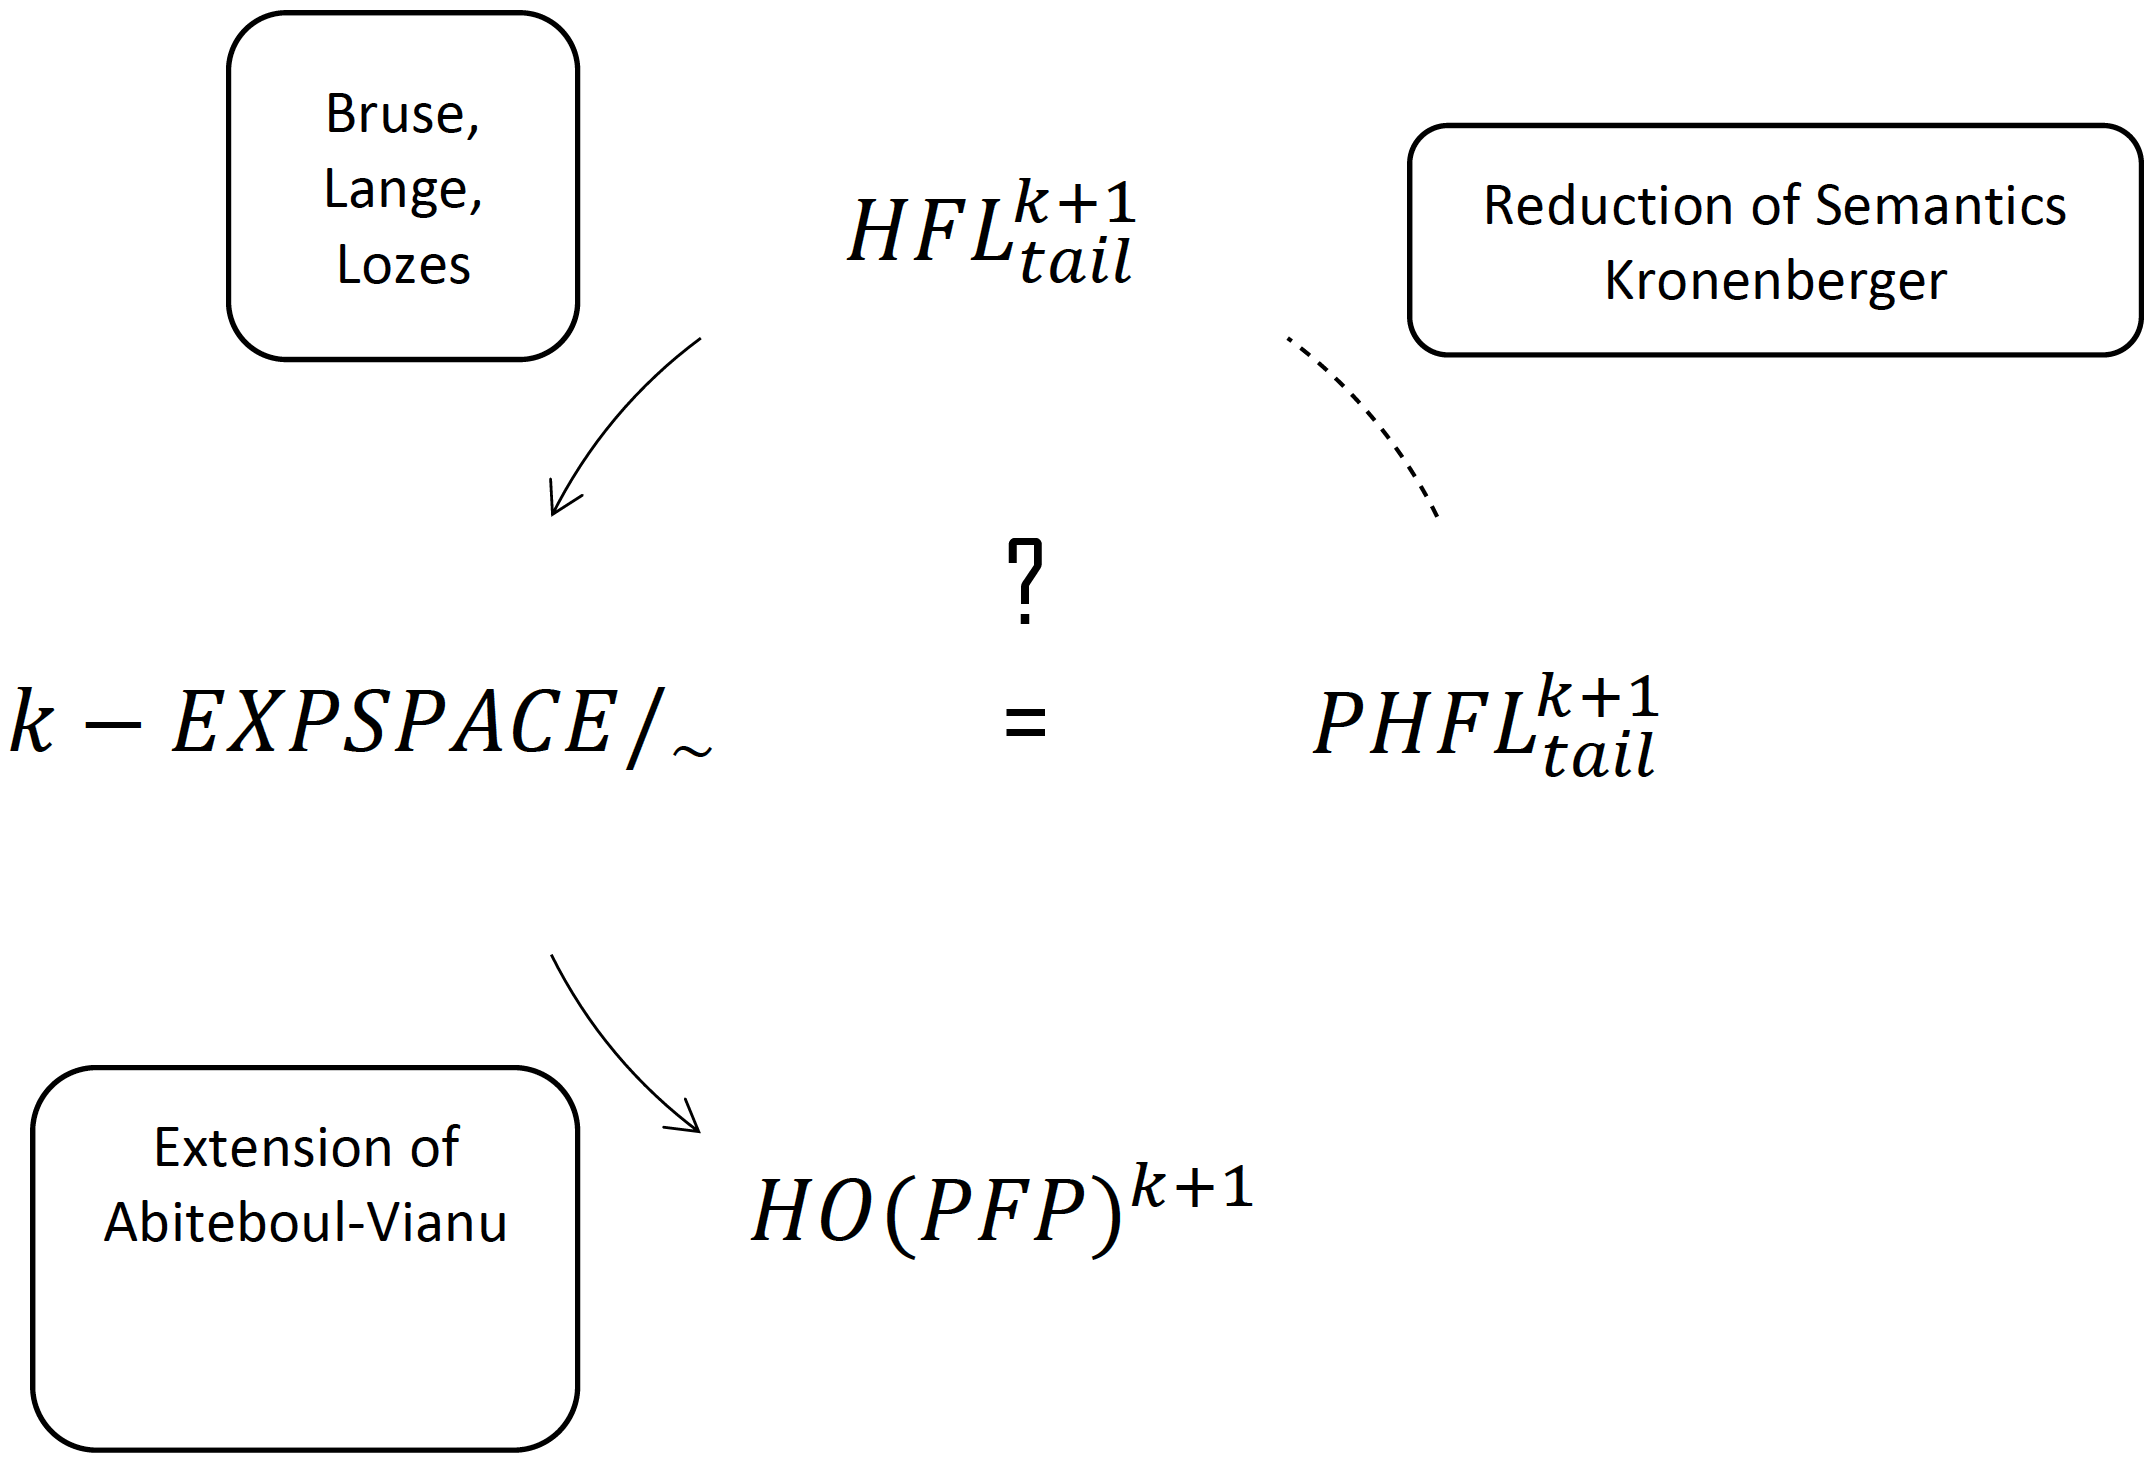
\includegraphics[width=0.9\textwidth]{phfl-tail_5.png}}
  \only<7>{\hspace{-0.6cm}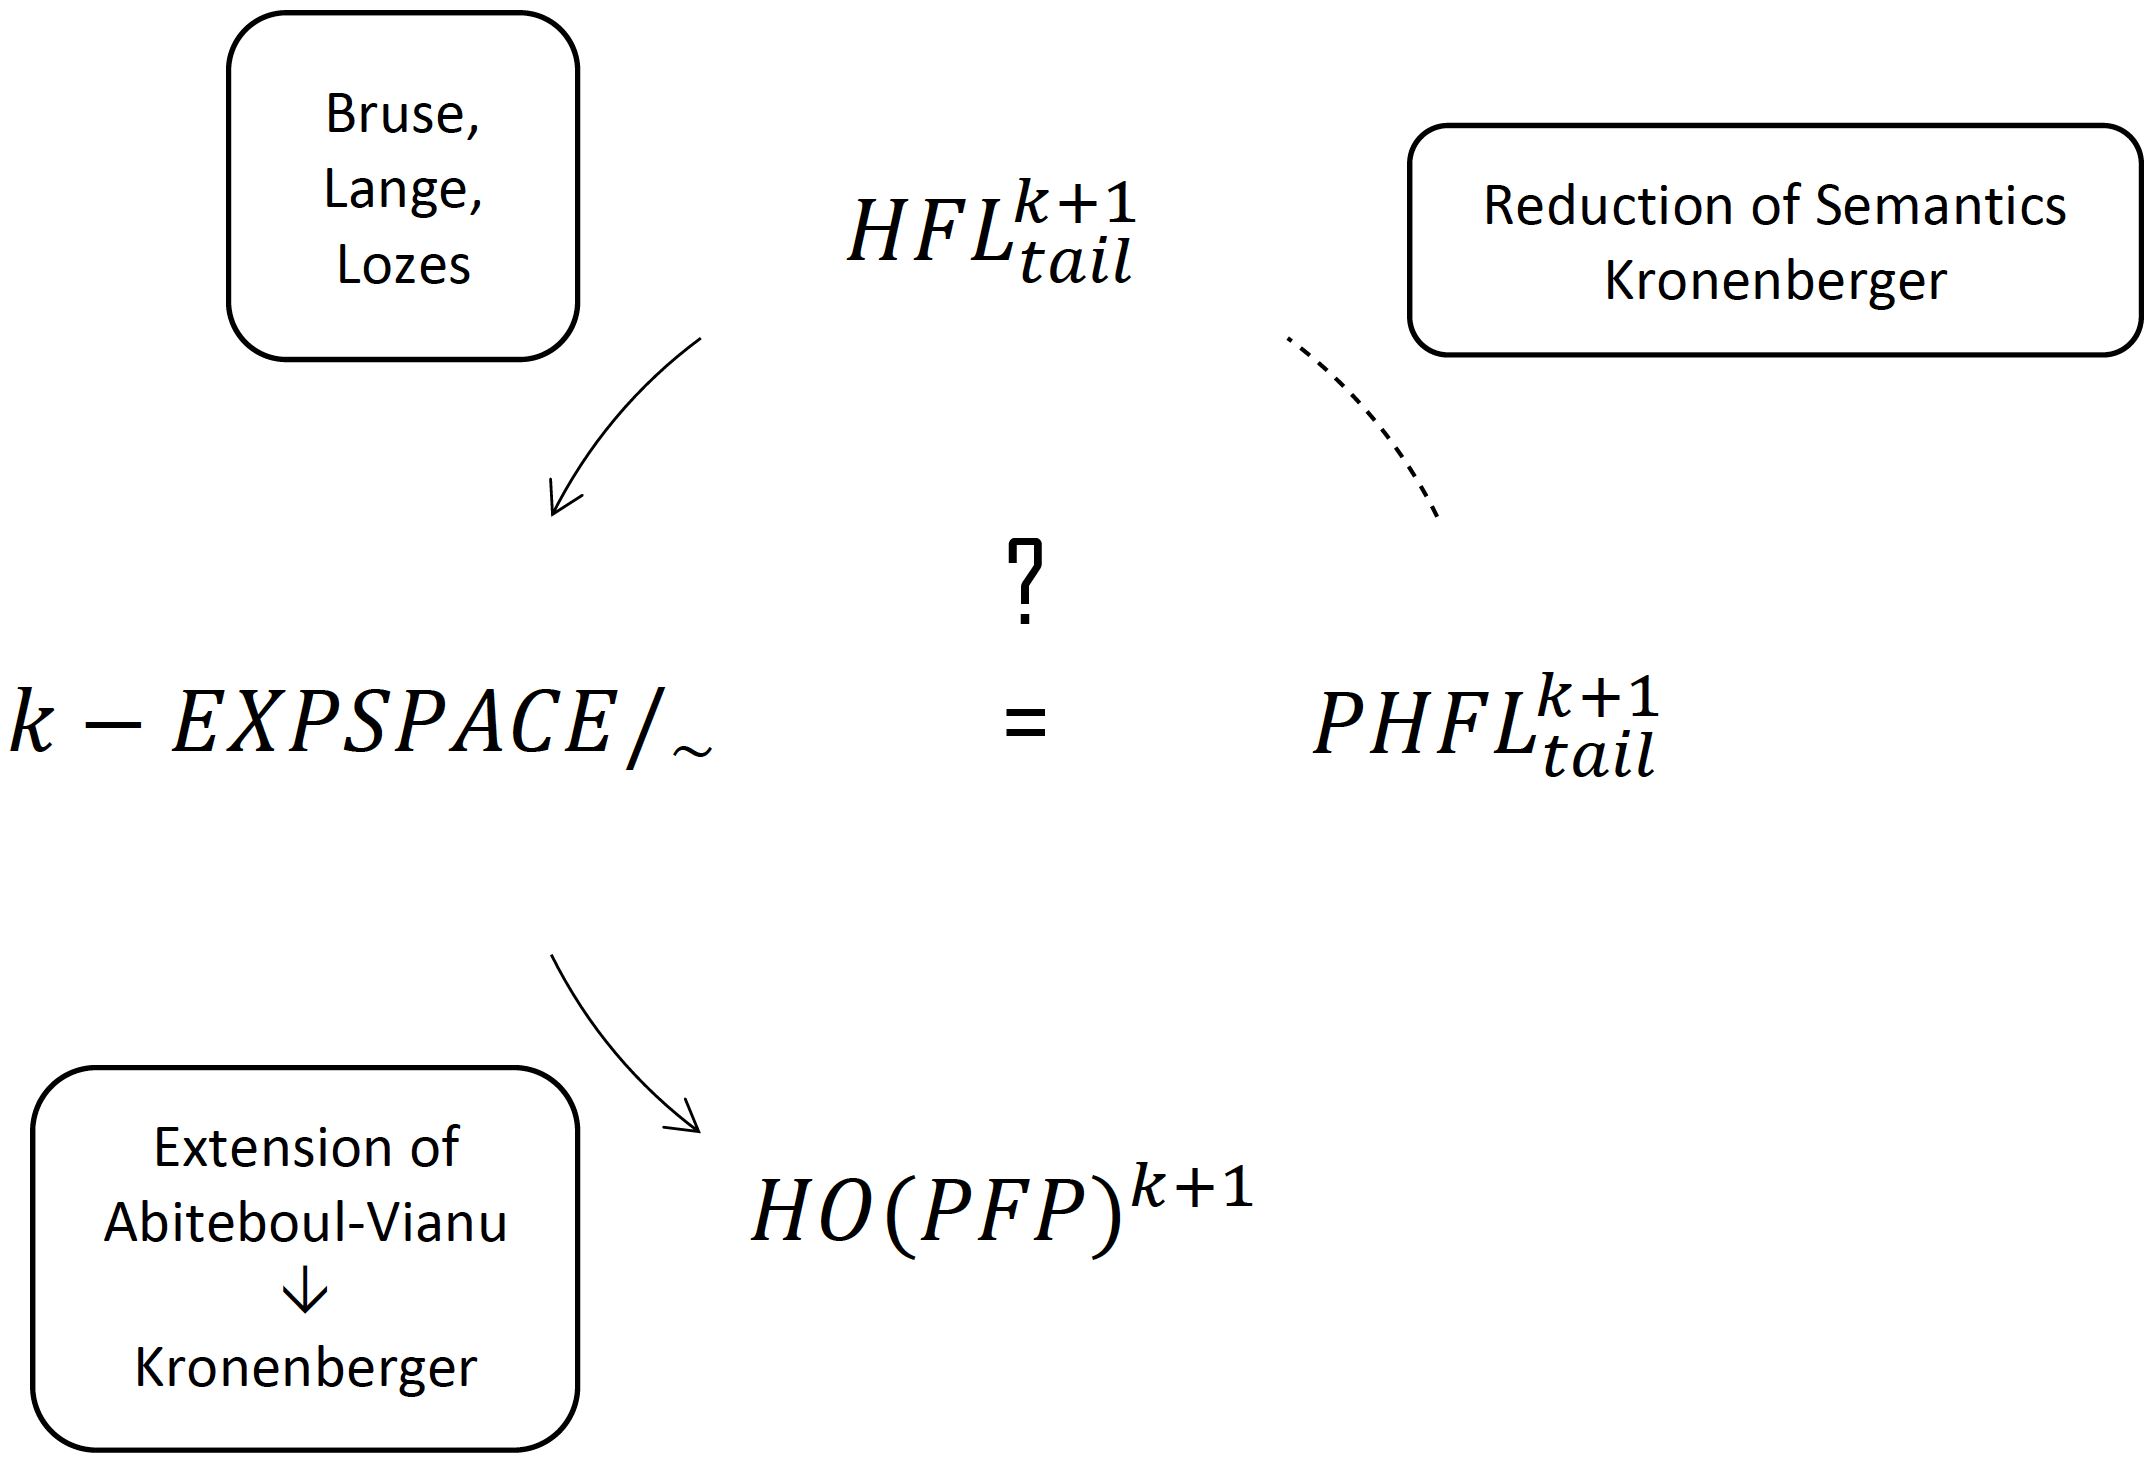
\includegraphics[width=0.9\textwidth]{phfl-tail_6.png}}
  \only<8>{\hspace{-0.7cm}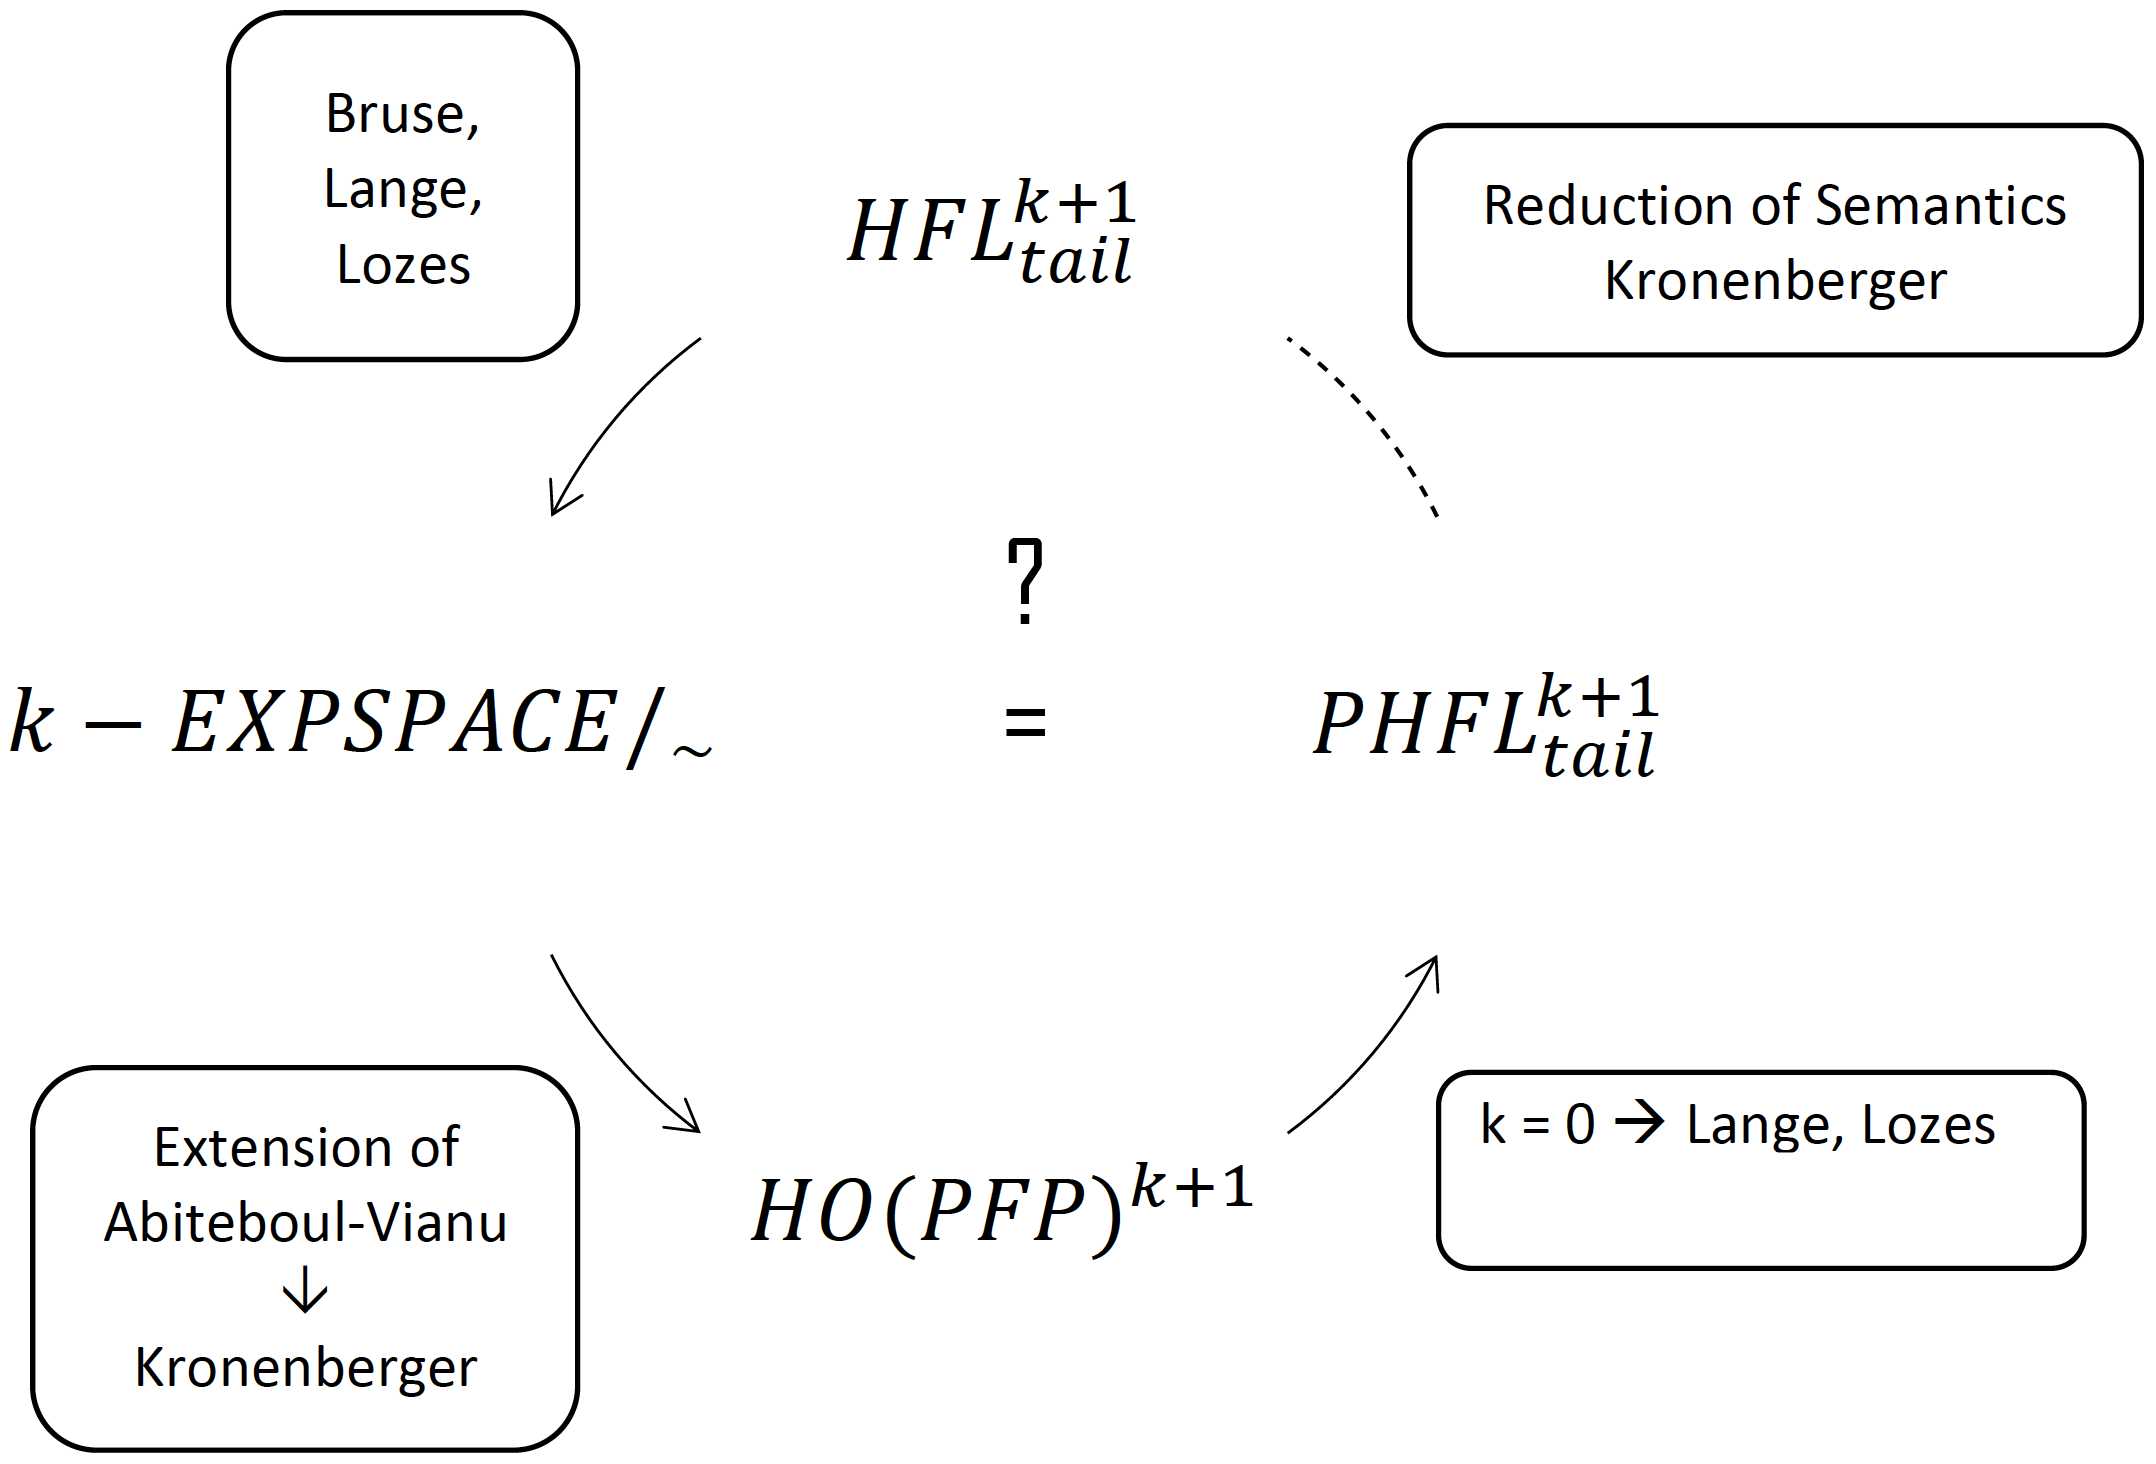
\includegraphics[width=0.9\textwidth]{phfl-tail_7.png}}
  \only<9>{\hspace{-0.8cm}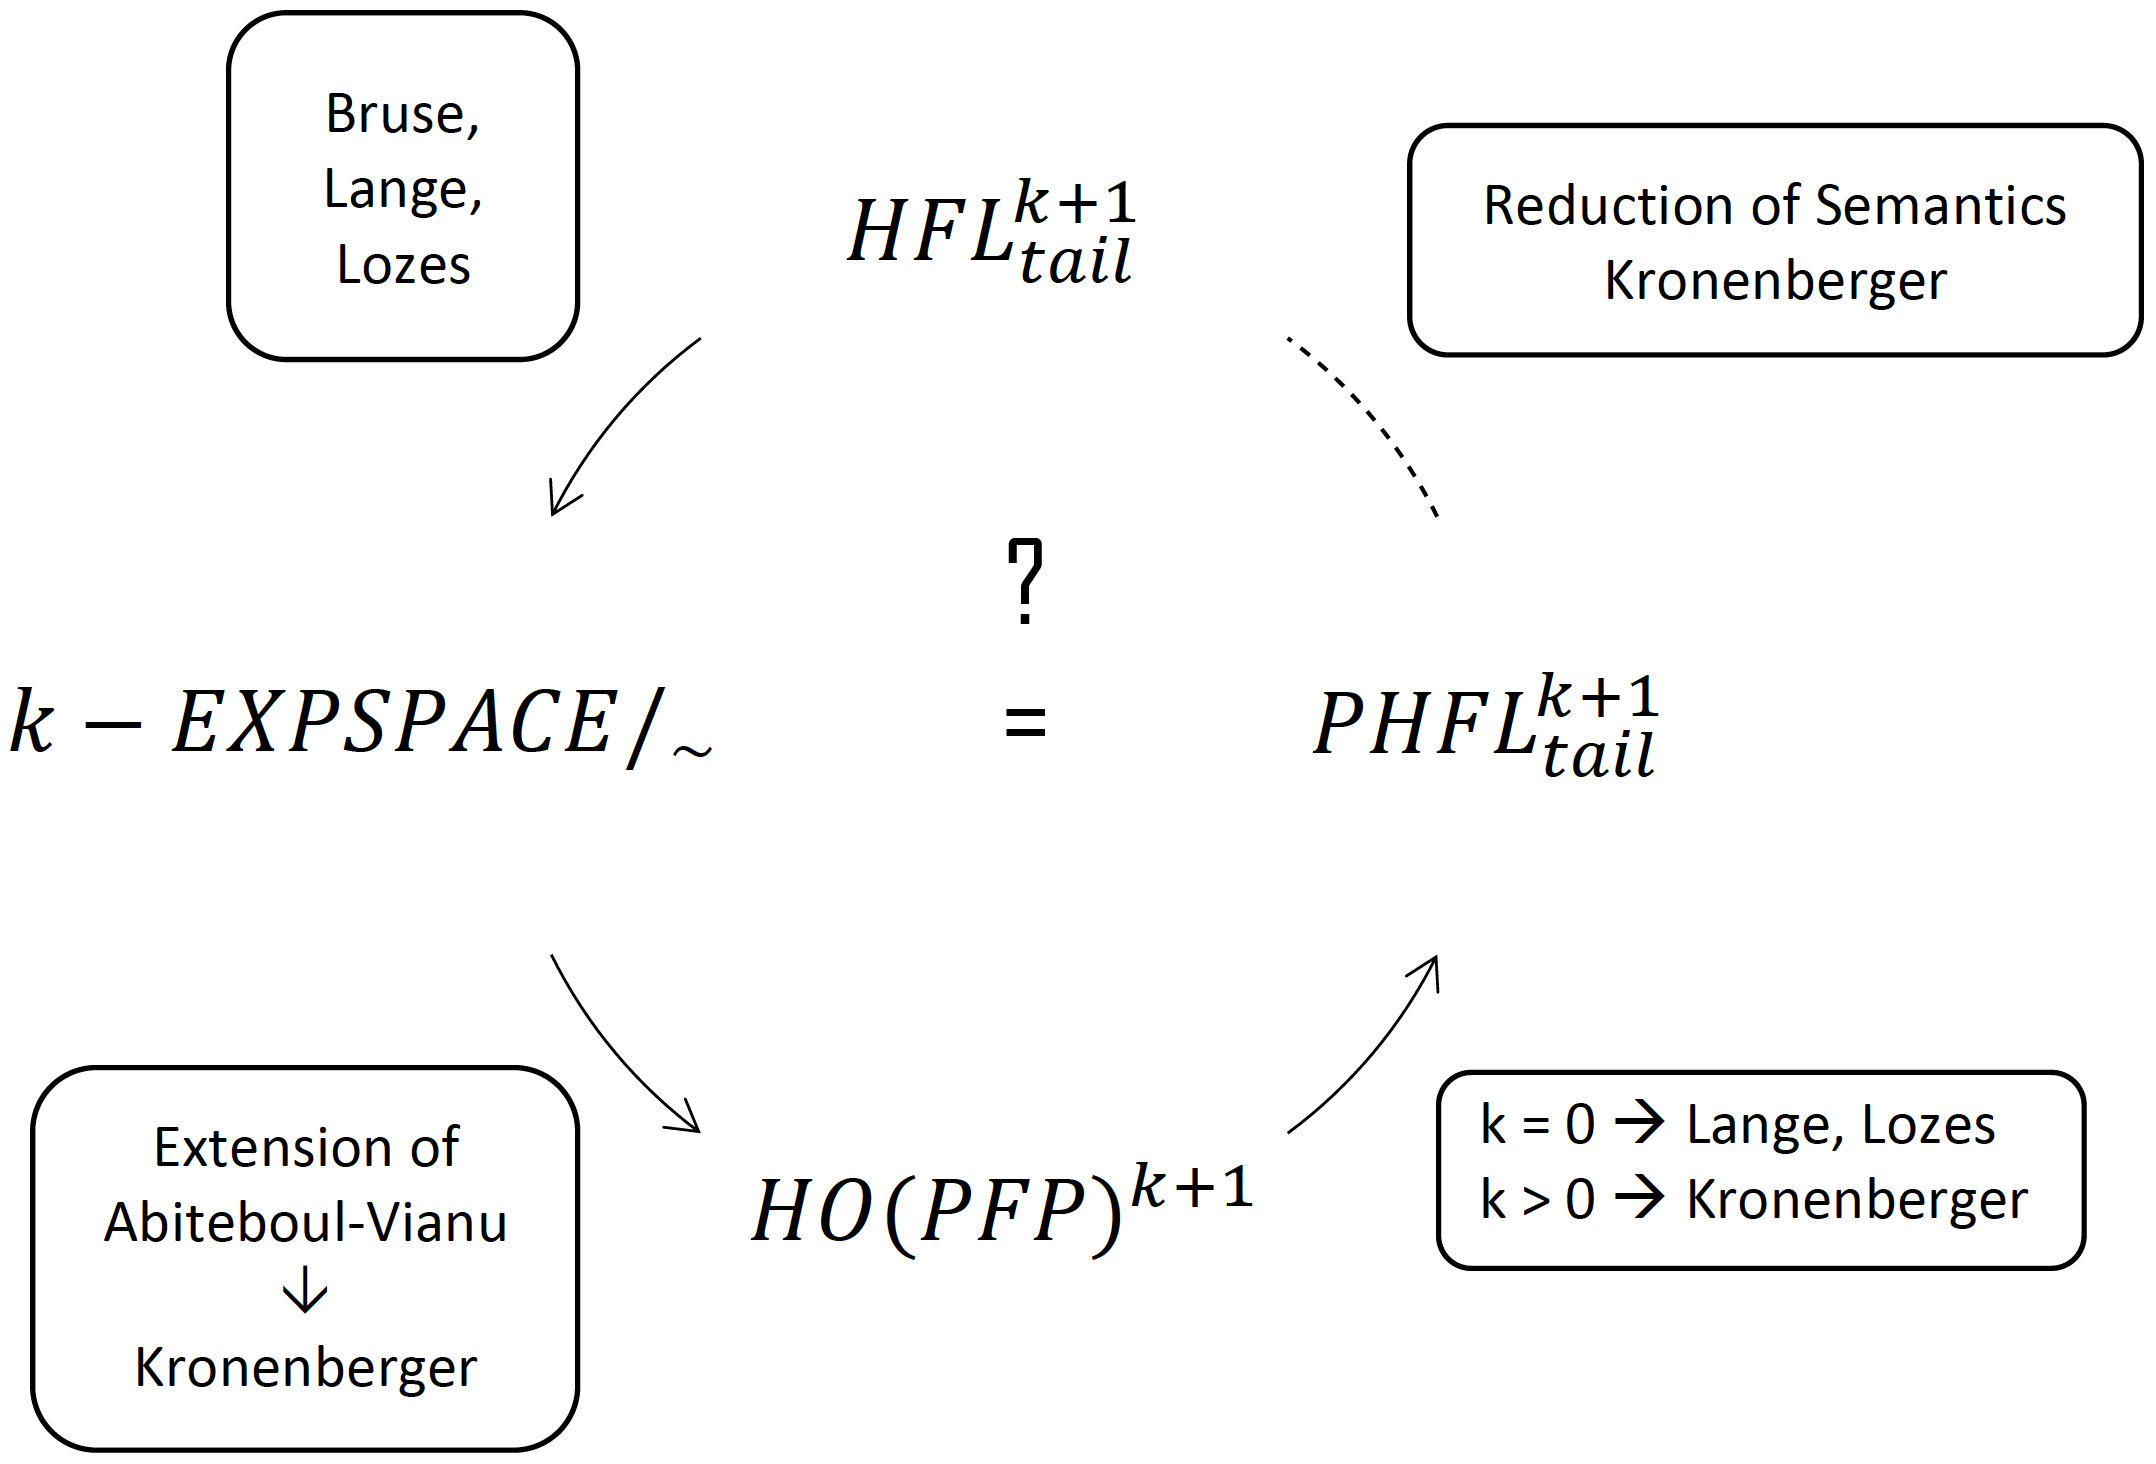
\includegraphics[width=0.9\textwidth]{phfl-tail_8.png}}
  \only<10>{\hspace{-0.9cm}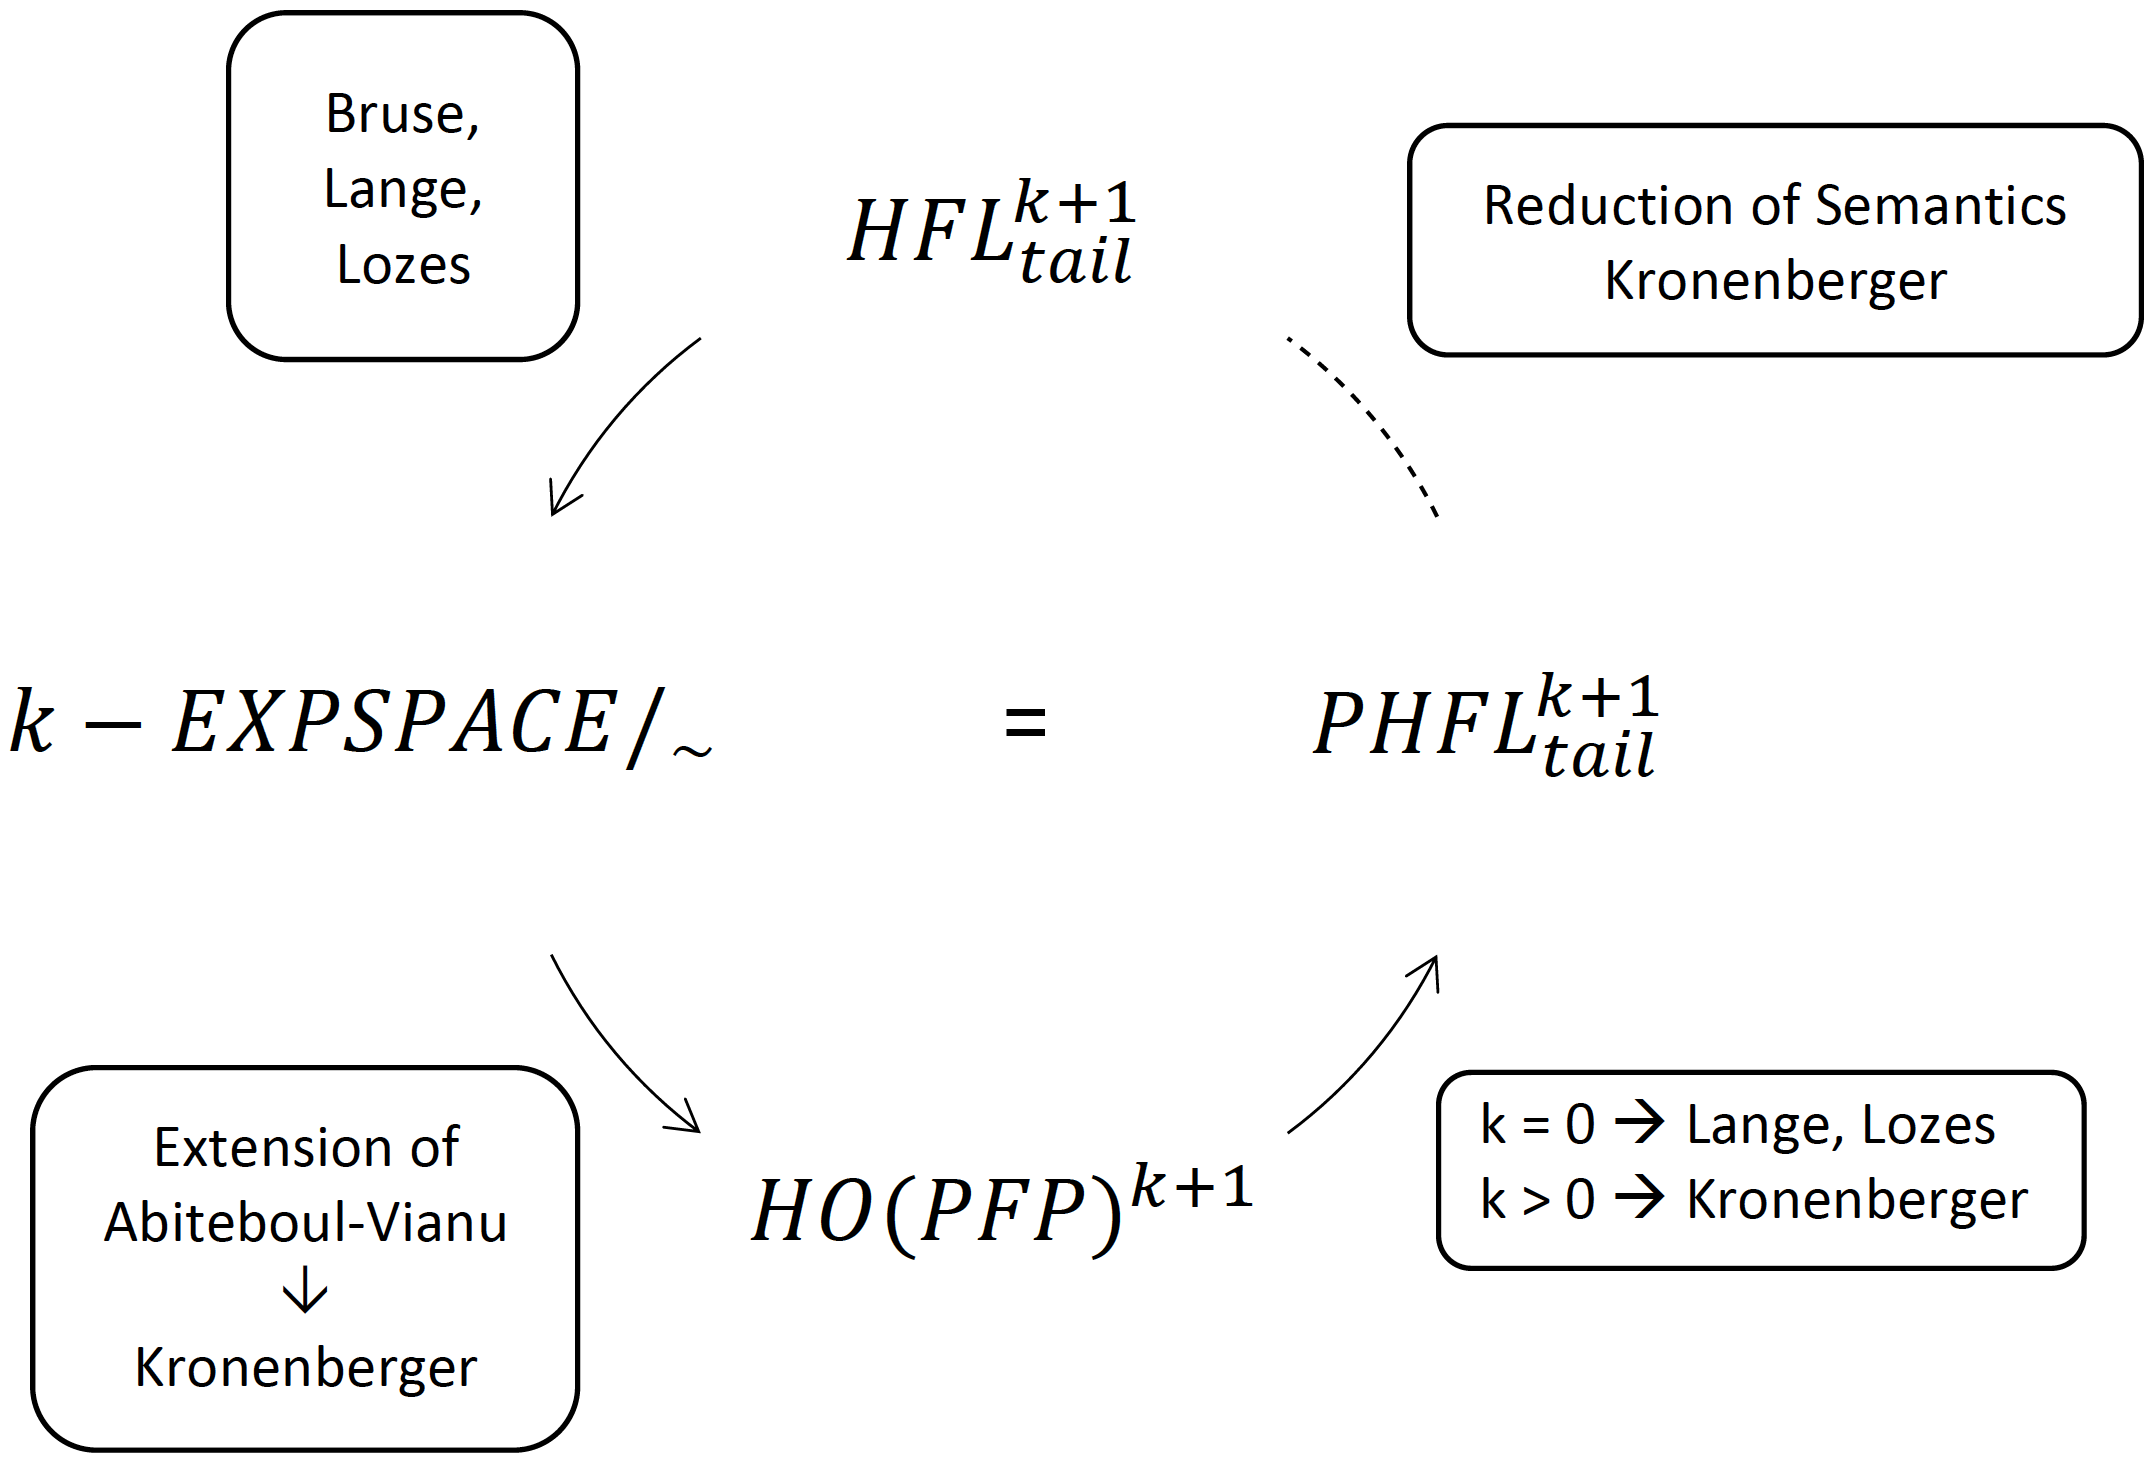
\includegraphics[width=0.9\textwidth]{phfl-tail.png}}}
\end{figure}

\end{frame}

\section{Quantifiers in PHFL}

\begin{frame}

\begin{compactenum}[$\bullet$]
\item<1-> No unrestricted quantifiers in PHFL
\item<3-> Needs order of domain
\item<4-> Creates successor of element
\item<2,5-> Iterate over all possible elements 
\end{compactenum}
\vspace{0.3cm}
\onslide<6-> We need orders of any domain
\begin{compactenum}[$\bullet$]
\item<7-> M. Otto defines a total order on states
\item<8-> Used to define lexicographic order
\item<9-> E. Lozes and M. Lange define successor for elements of base type
\end{compactenum}
\end{frame}
\begin{frame}

\begin{figure}[ht]
	\centering{
  \only<1>{\hspace{-0.1cm}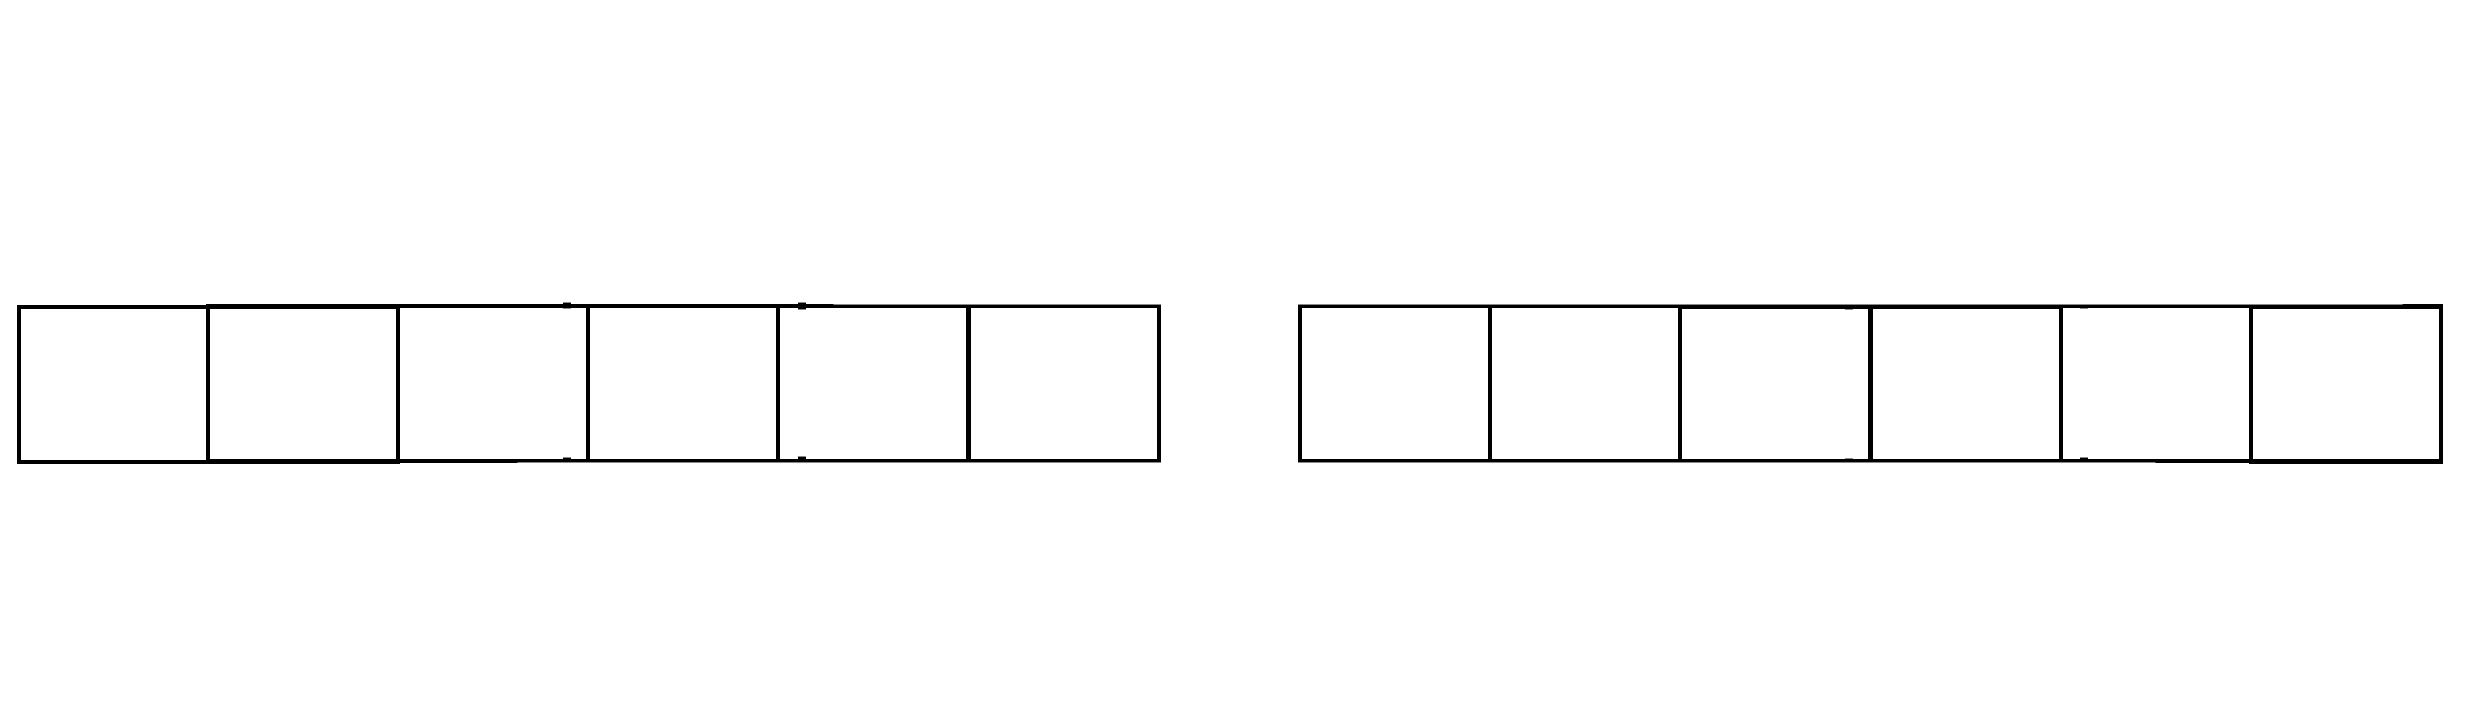
\includegraphics[width=0.9\textwidth]{less-tuple_0.png}}
  \only<2>{\hspace{-0.1cm}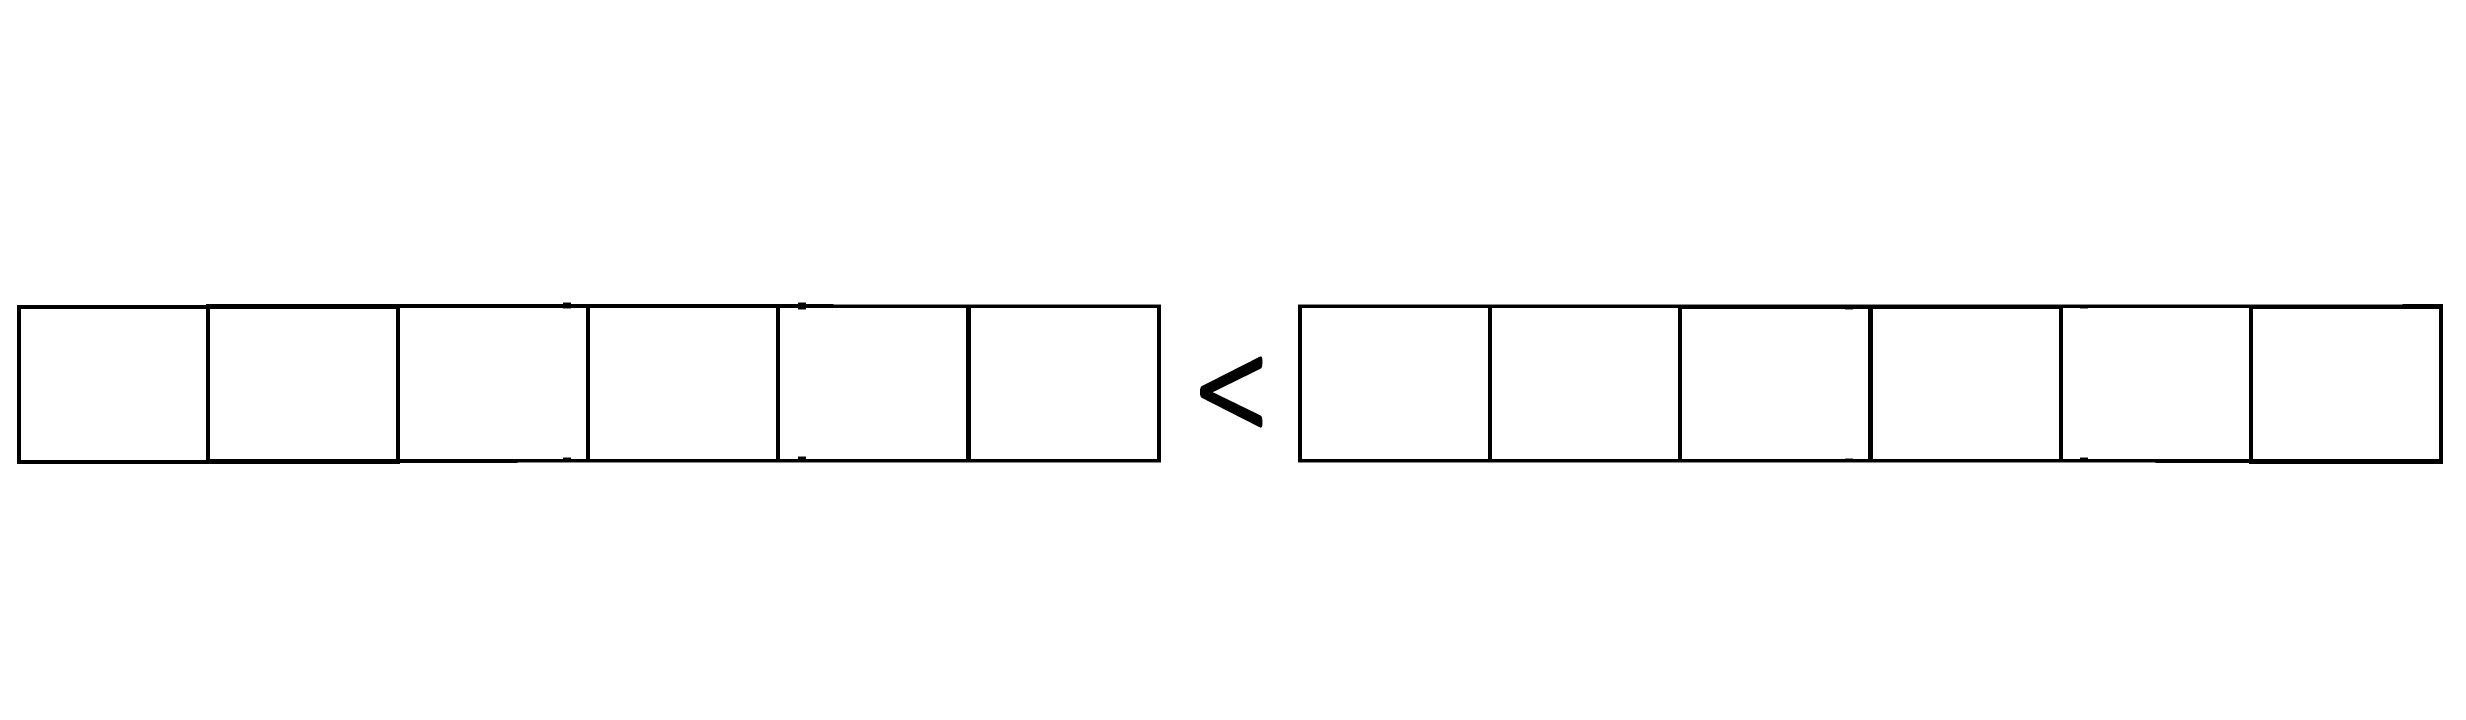
\includegraphics[width=0.9\textwidth]{less-tuple_1.png}}
  \only<3>{\hspace{-0.2cm}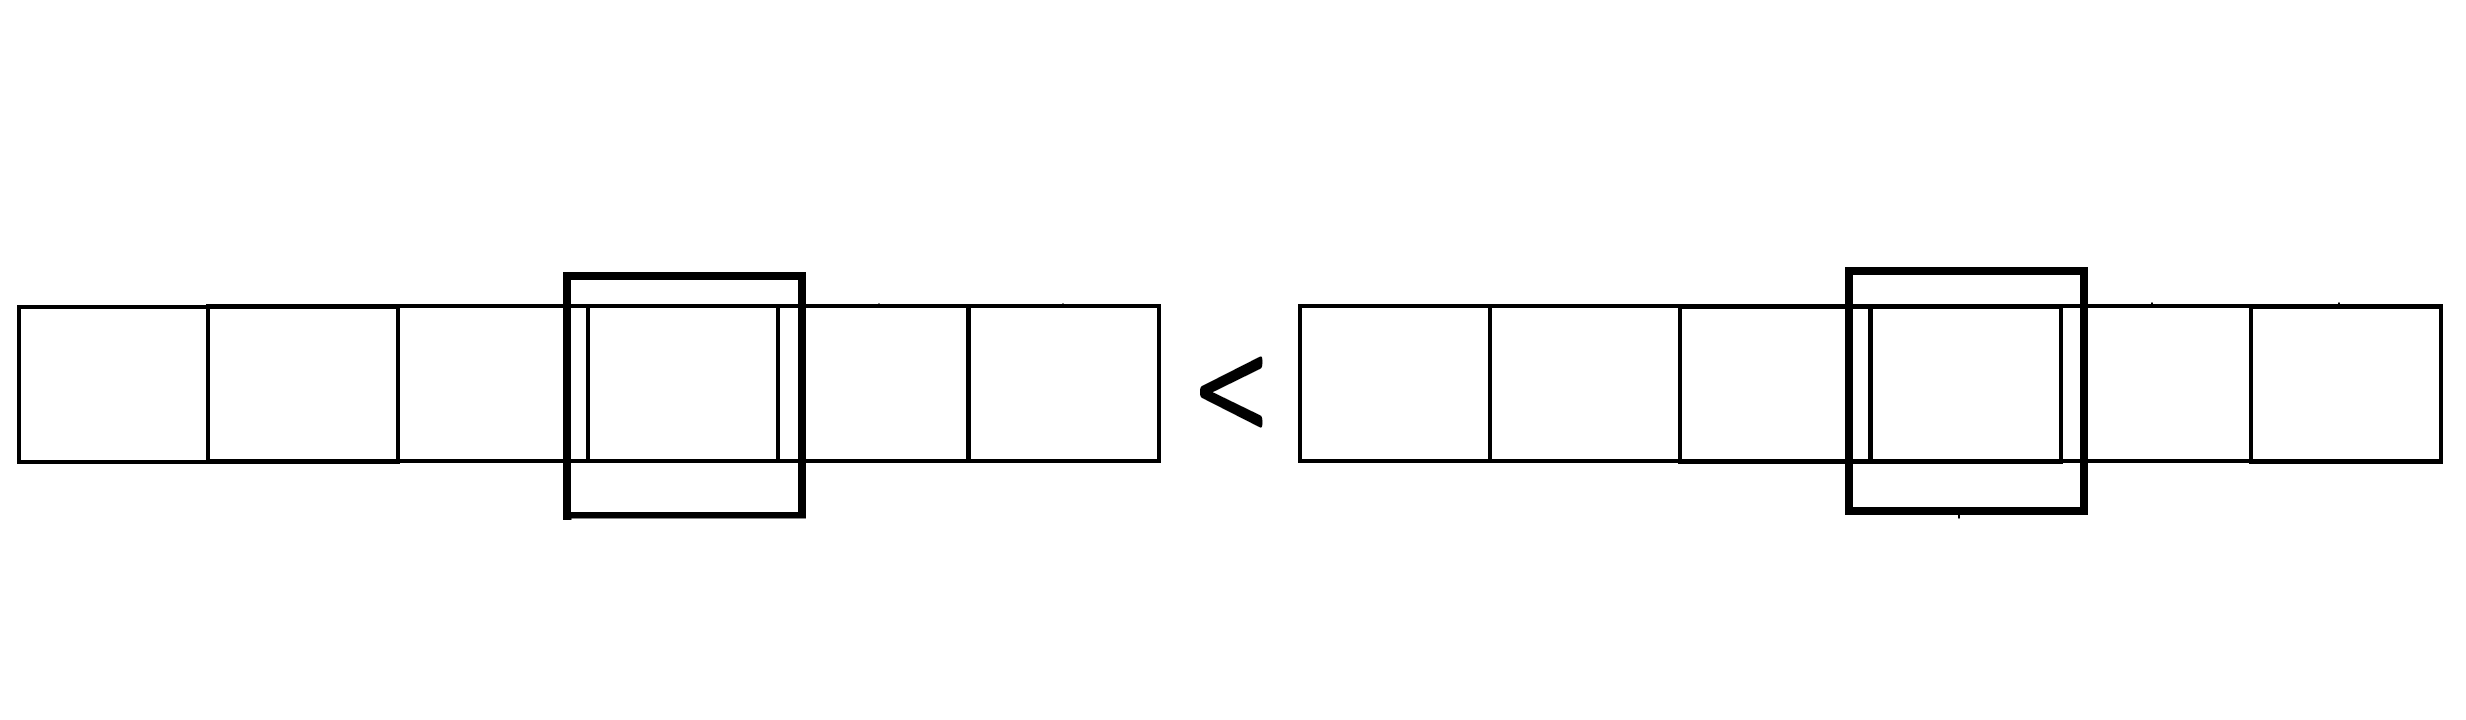
\includegraphics[width=0.9\textwidth]{less-tuple_2.png}}
   \only<4>{\hspace{-0.3cm}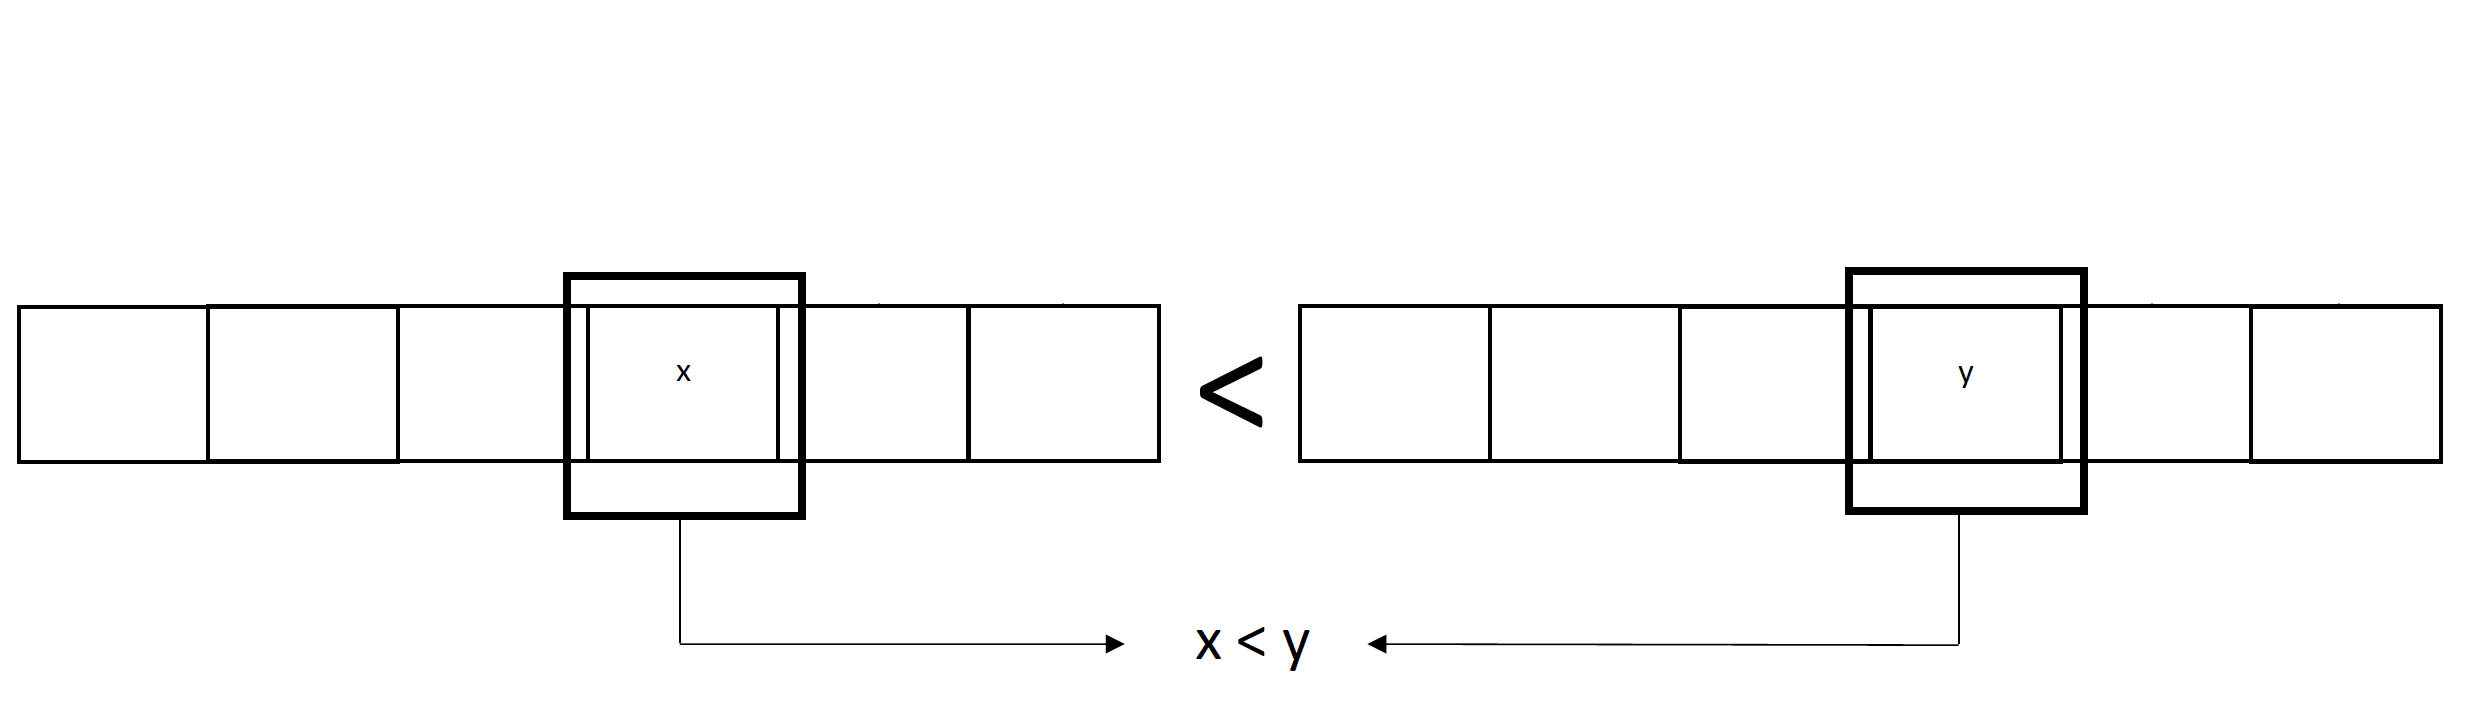
\includegraphics[width=0.9\textwidth]{less-tuple_3.png}}
  \only<5>{\hspace{-0.4cm}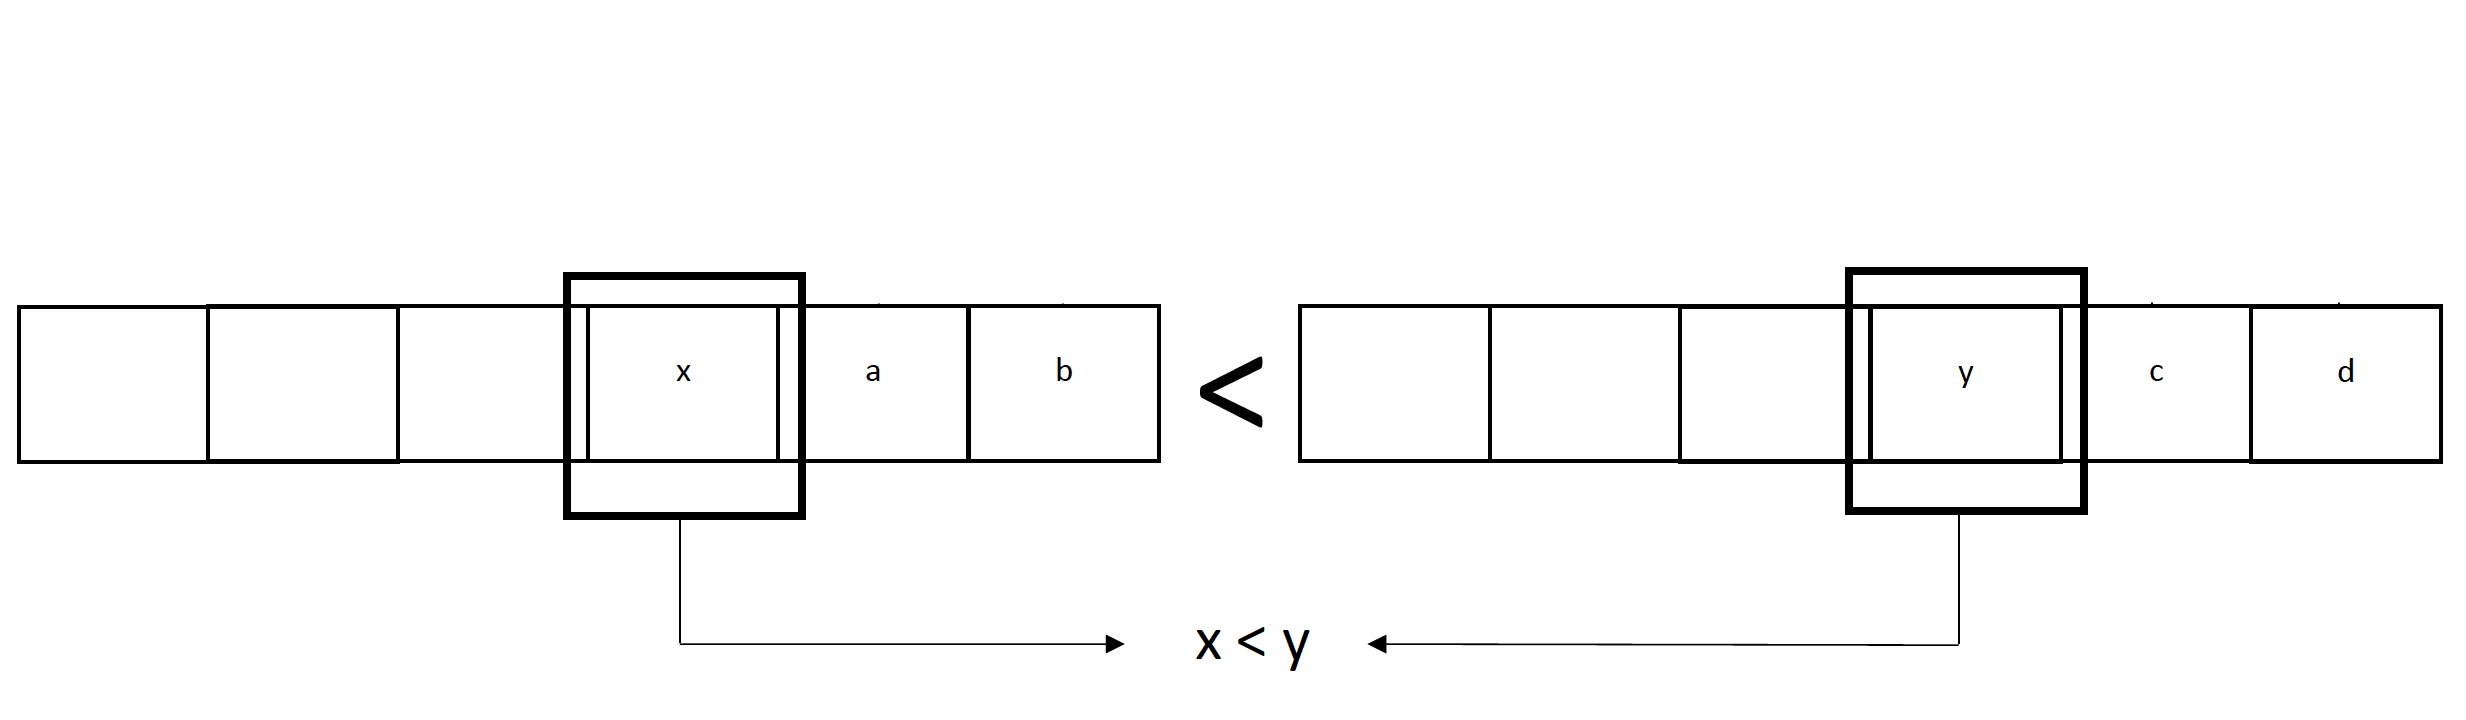
\includegraphics[width=0.9\textwidth]{less-tuple_4.png}}
  \only<6>{\hspace{-0.5cm}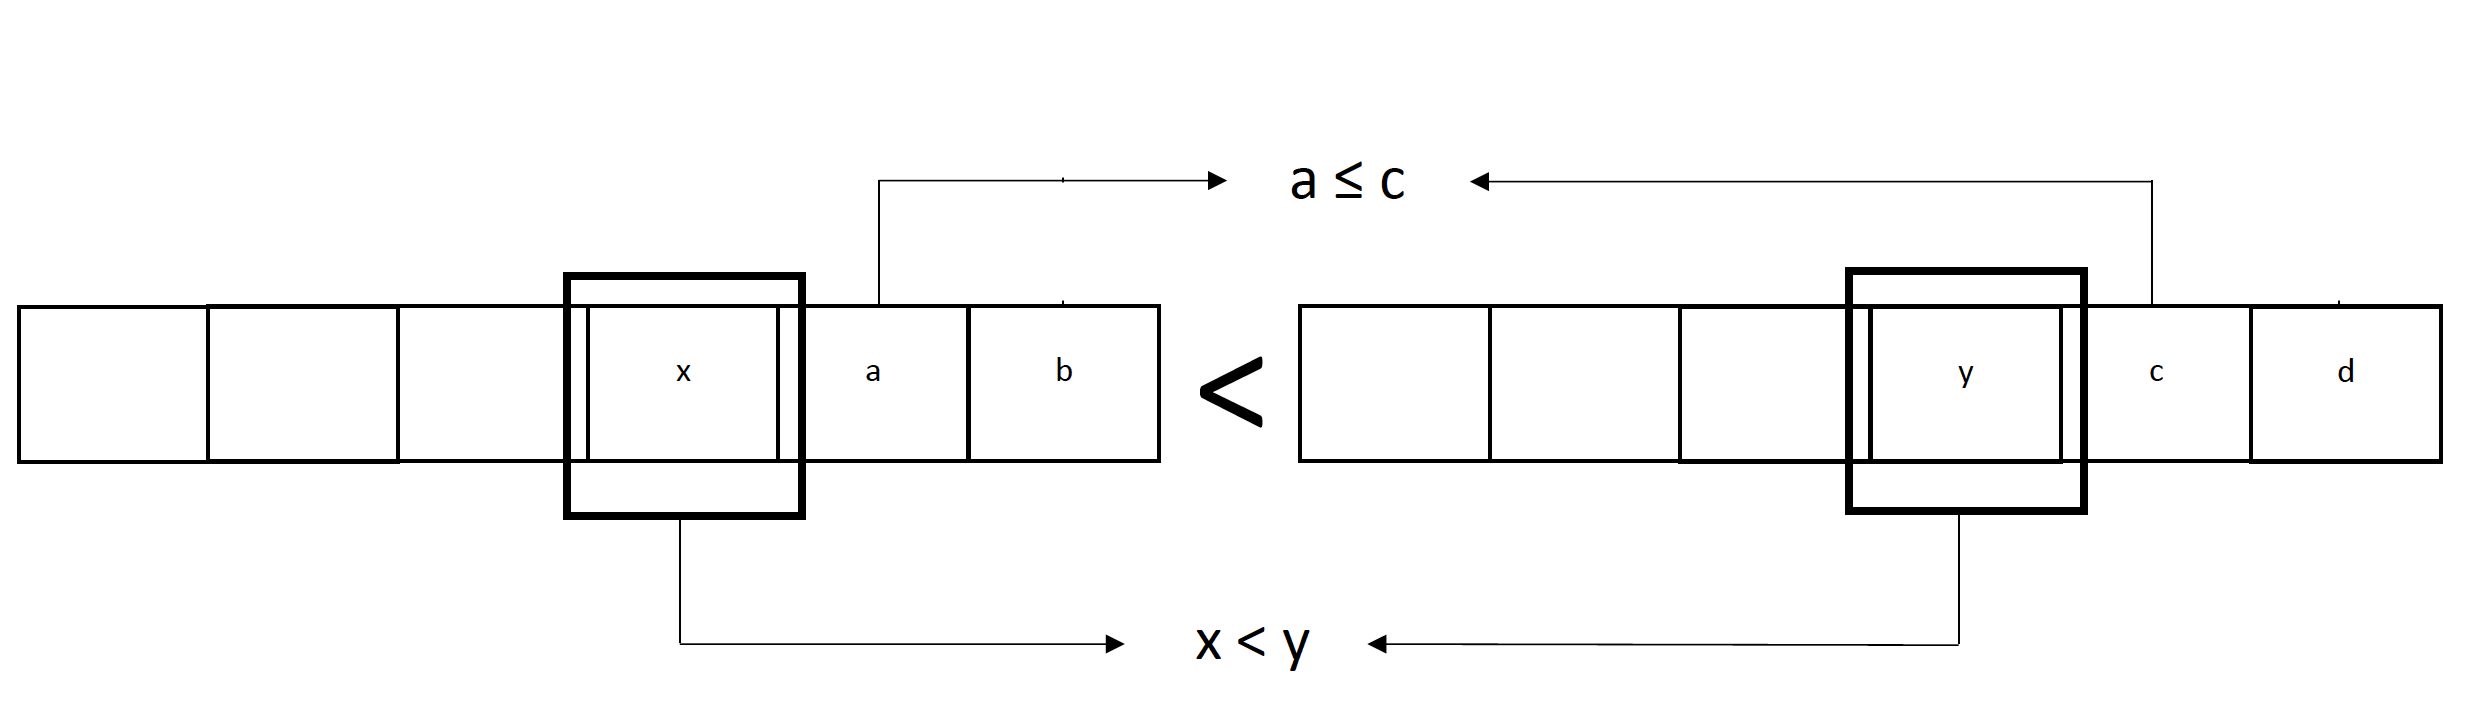
\includegraphics[width=0.9\textwidth]{less-tuple_5.png}}
  \only<7>{\hspace{-0.6cm}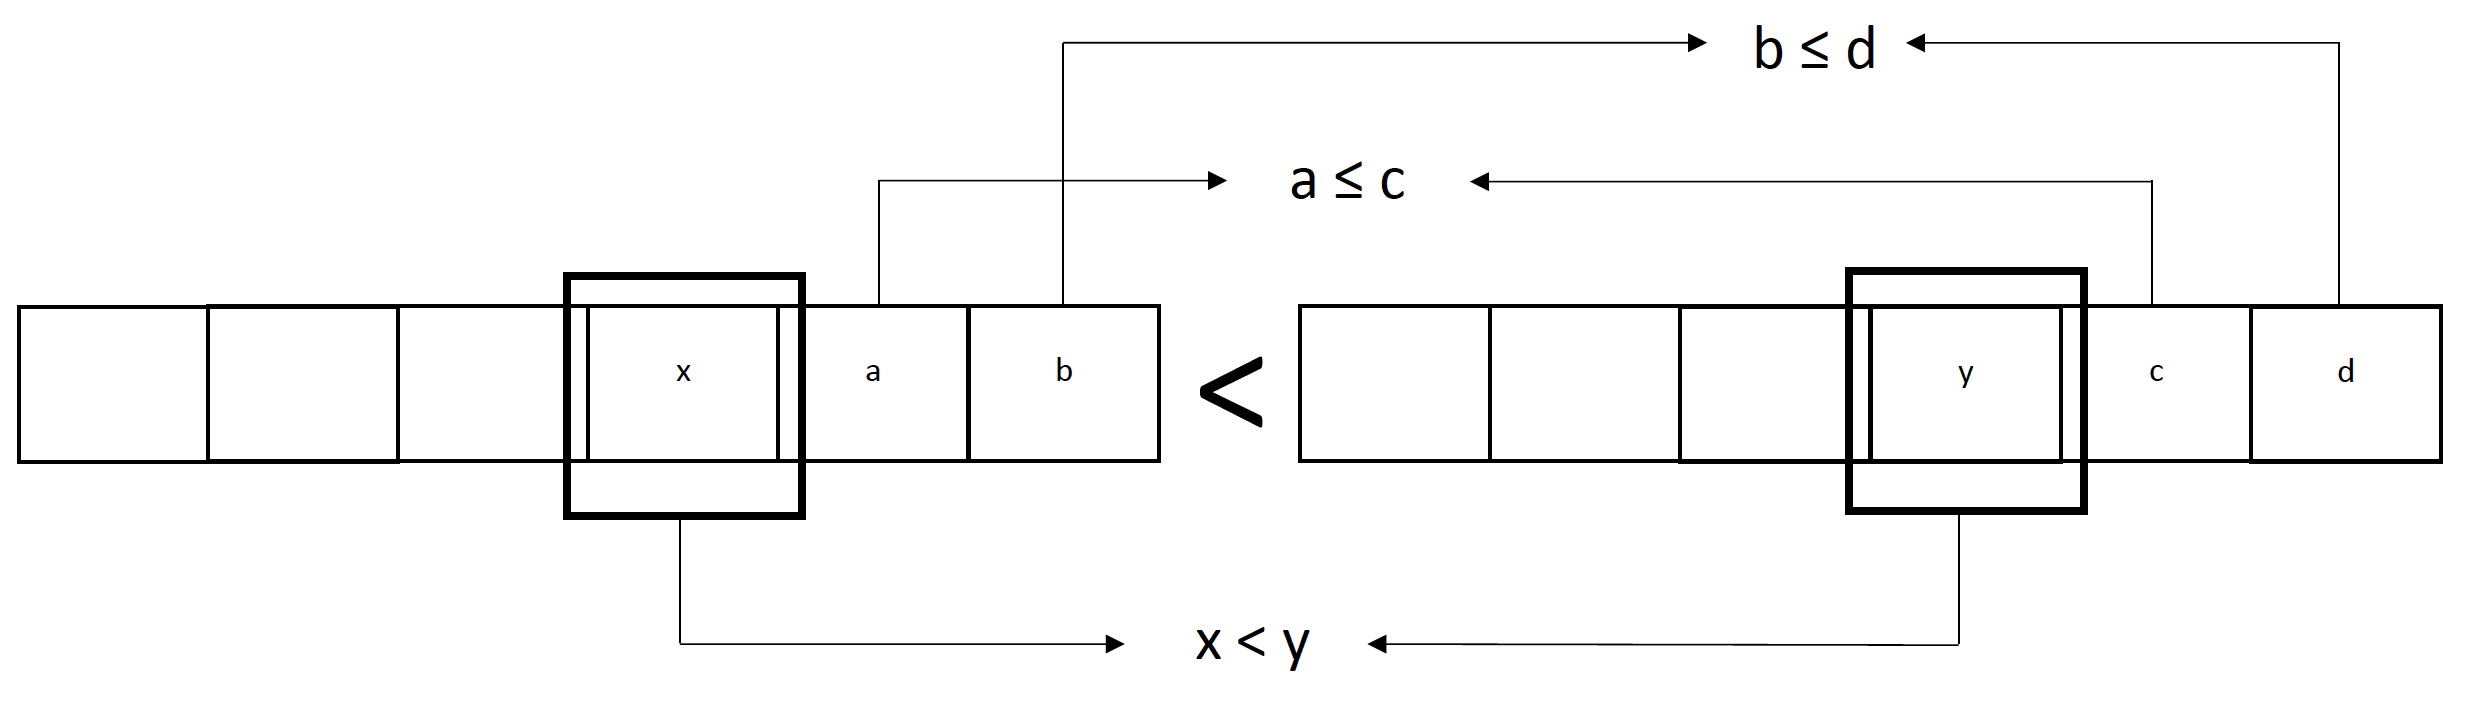
\includegraphics[width=0.9\textwidth]{less-tuple.png}}}
\end{figure}

\end{frame}
\begin{frame}

\begin{figure}[ht]
	\centering{
  \only<1>{\hspace{-0.1cm}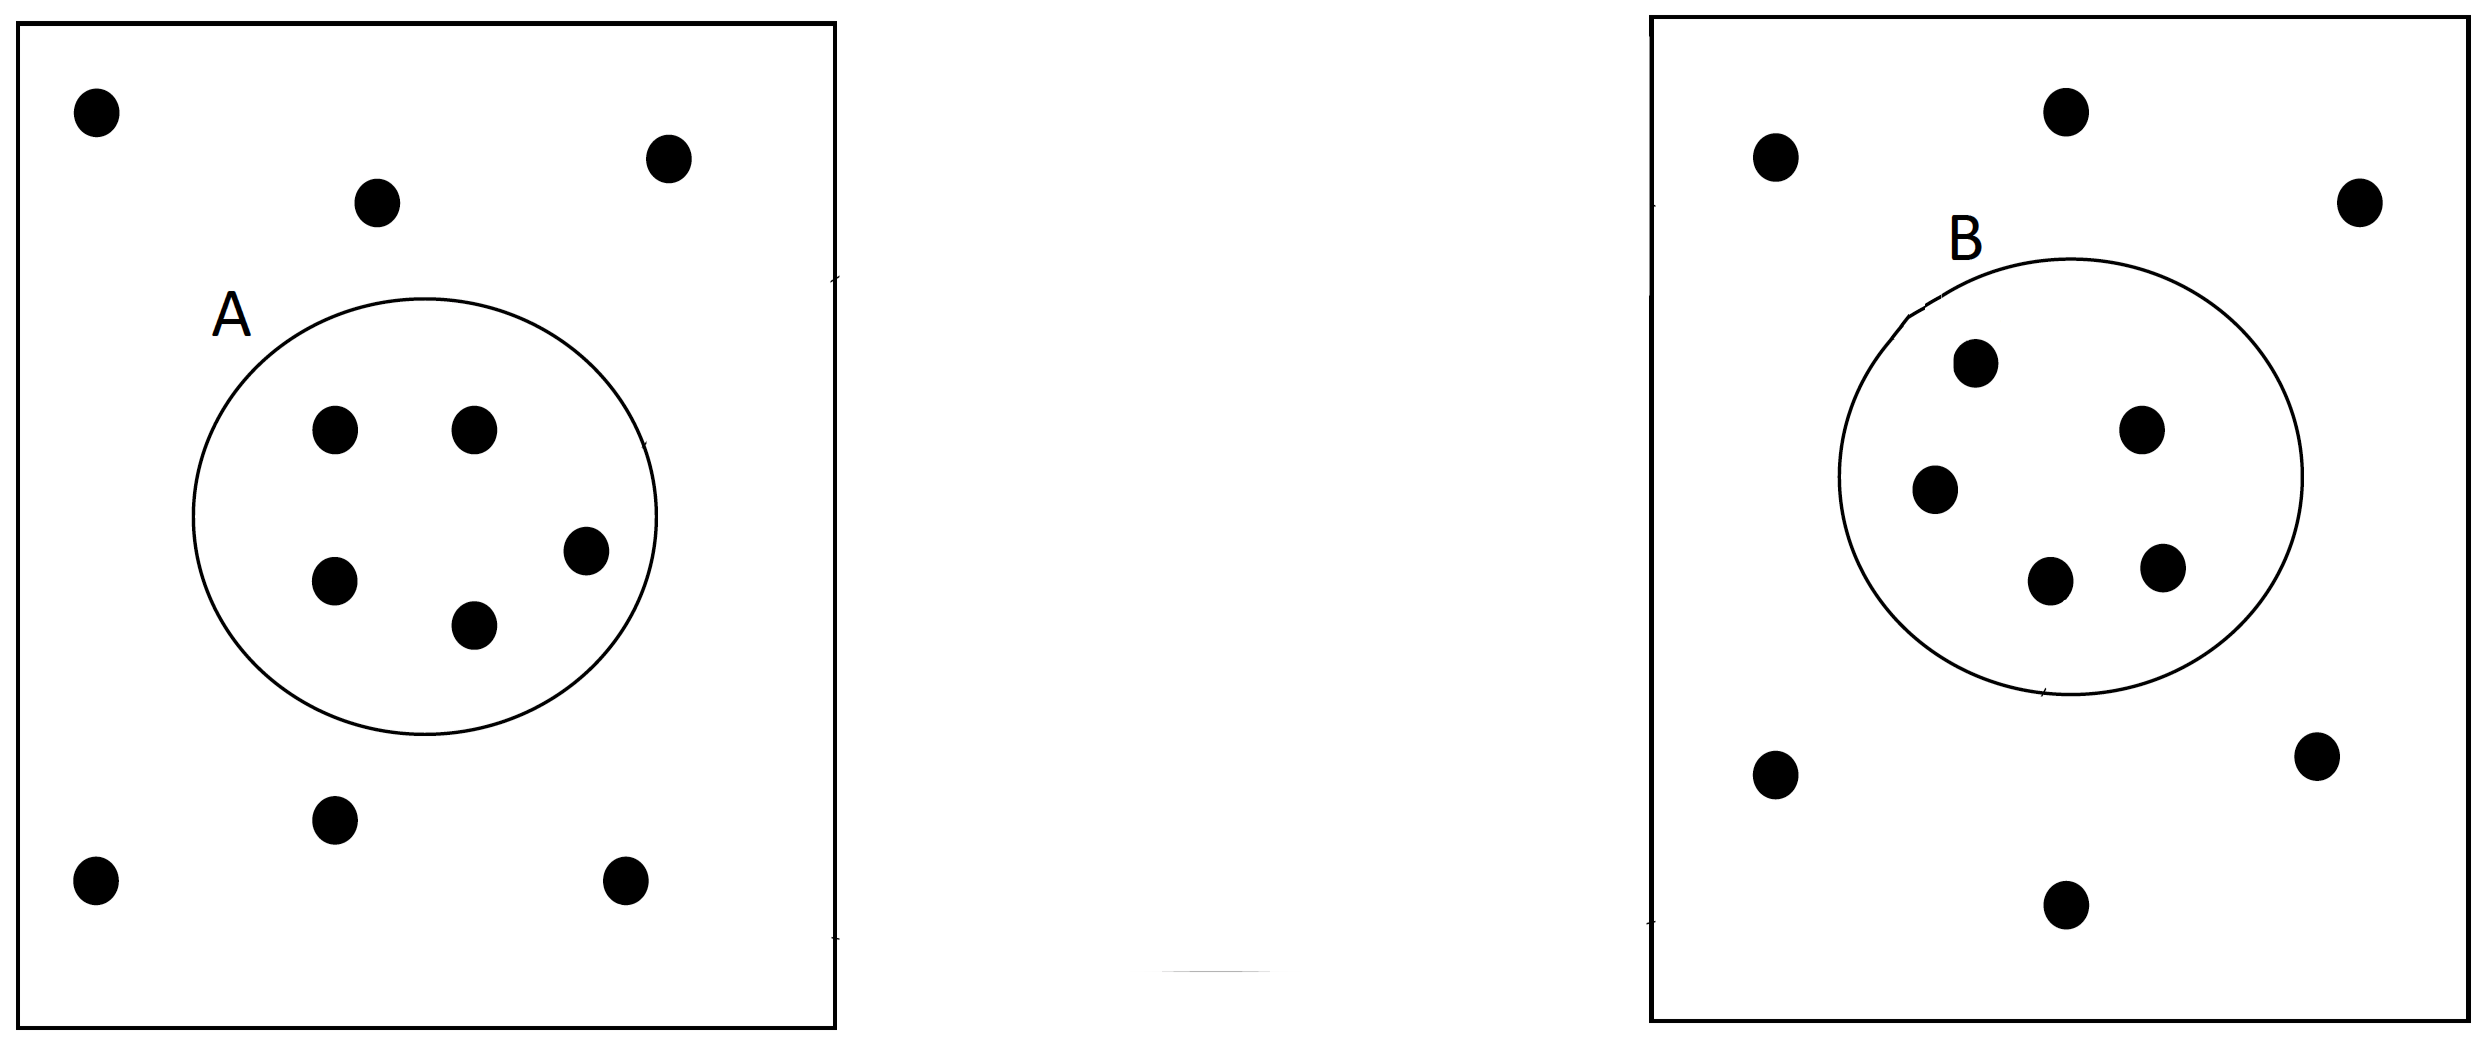
\includegraphics[width=0.9\textwidth]{less-set_0.png}}
  \only<2>{\hspace{-0.1cm}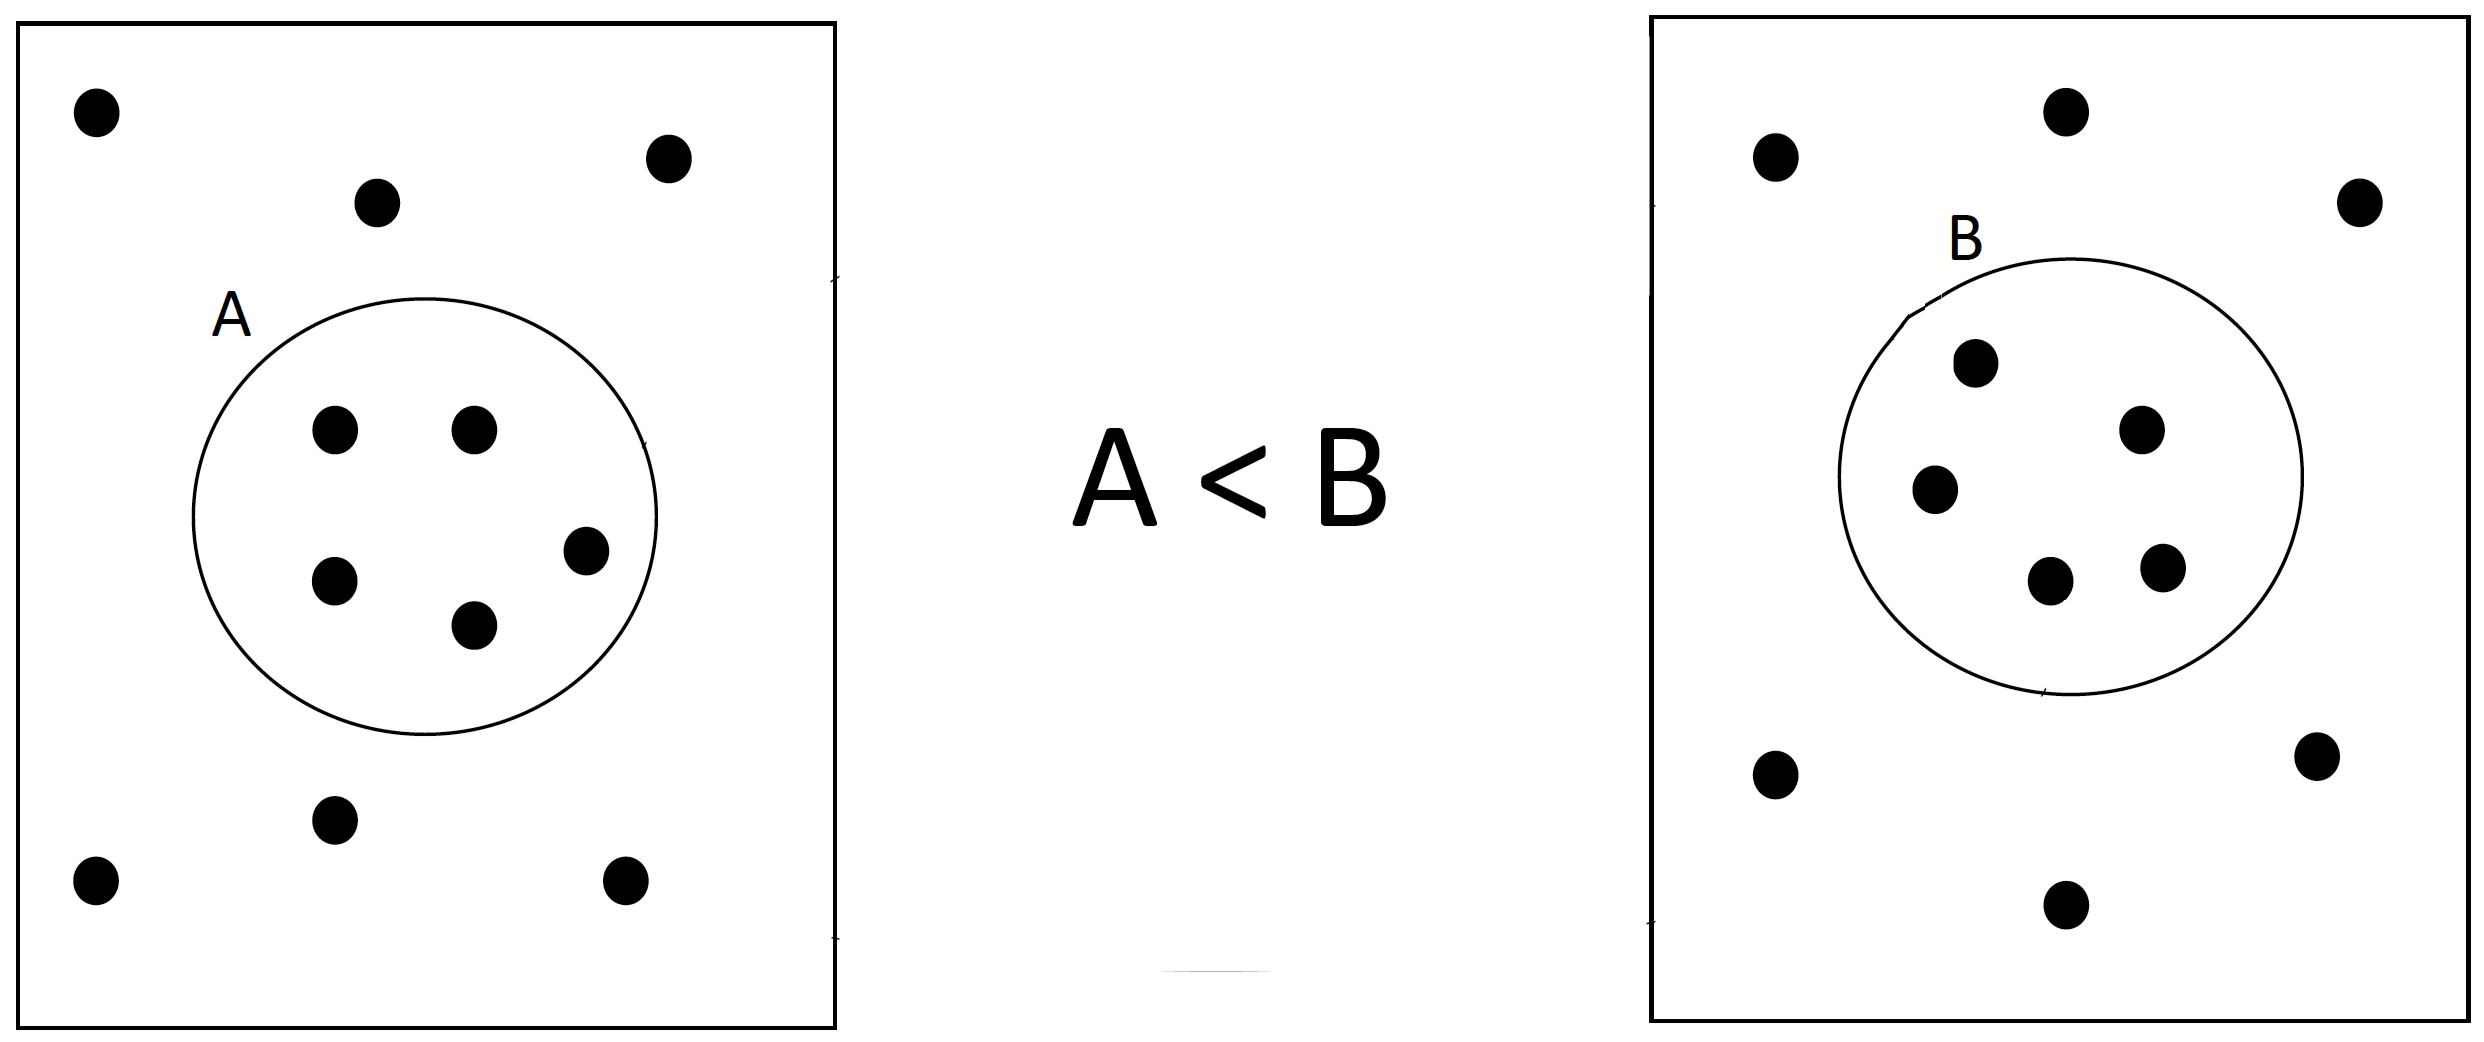
\includegraphics[width=0.9\textwidth]{less-set_1.png}}
  \only<3>{\hspace{-0.2cm}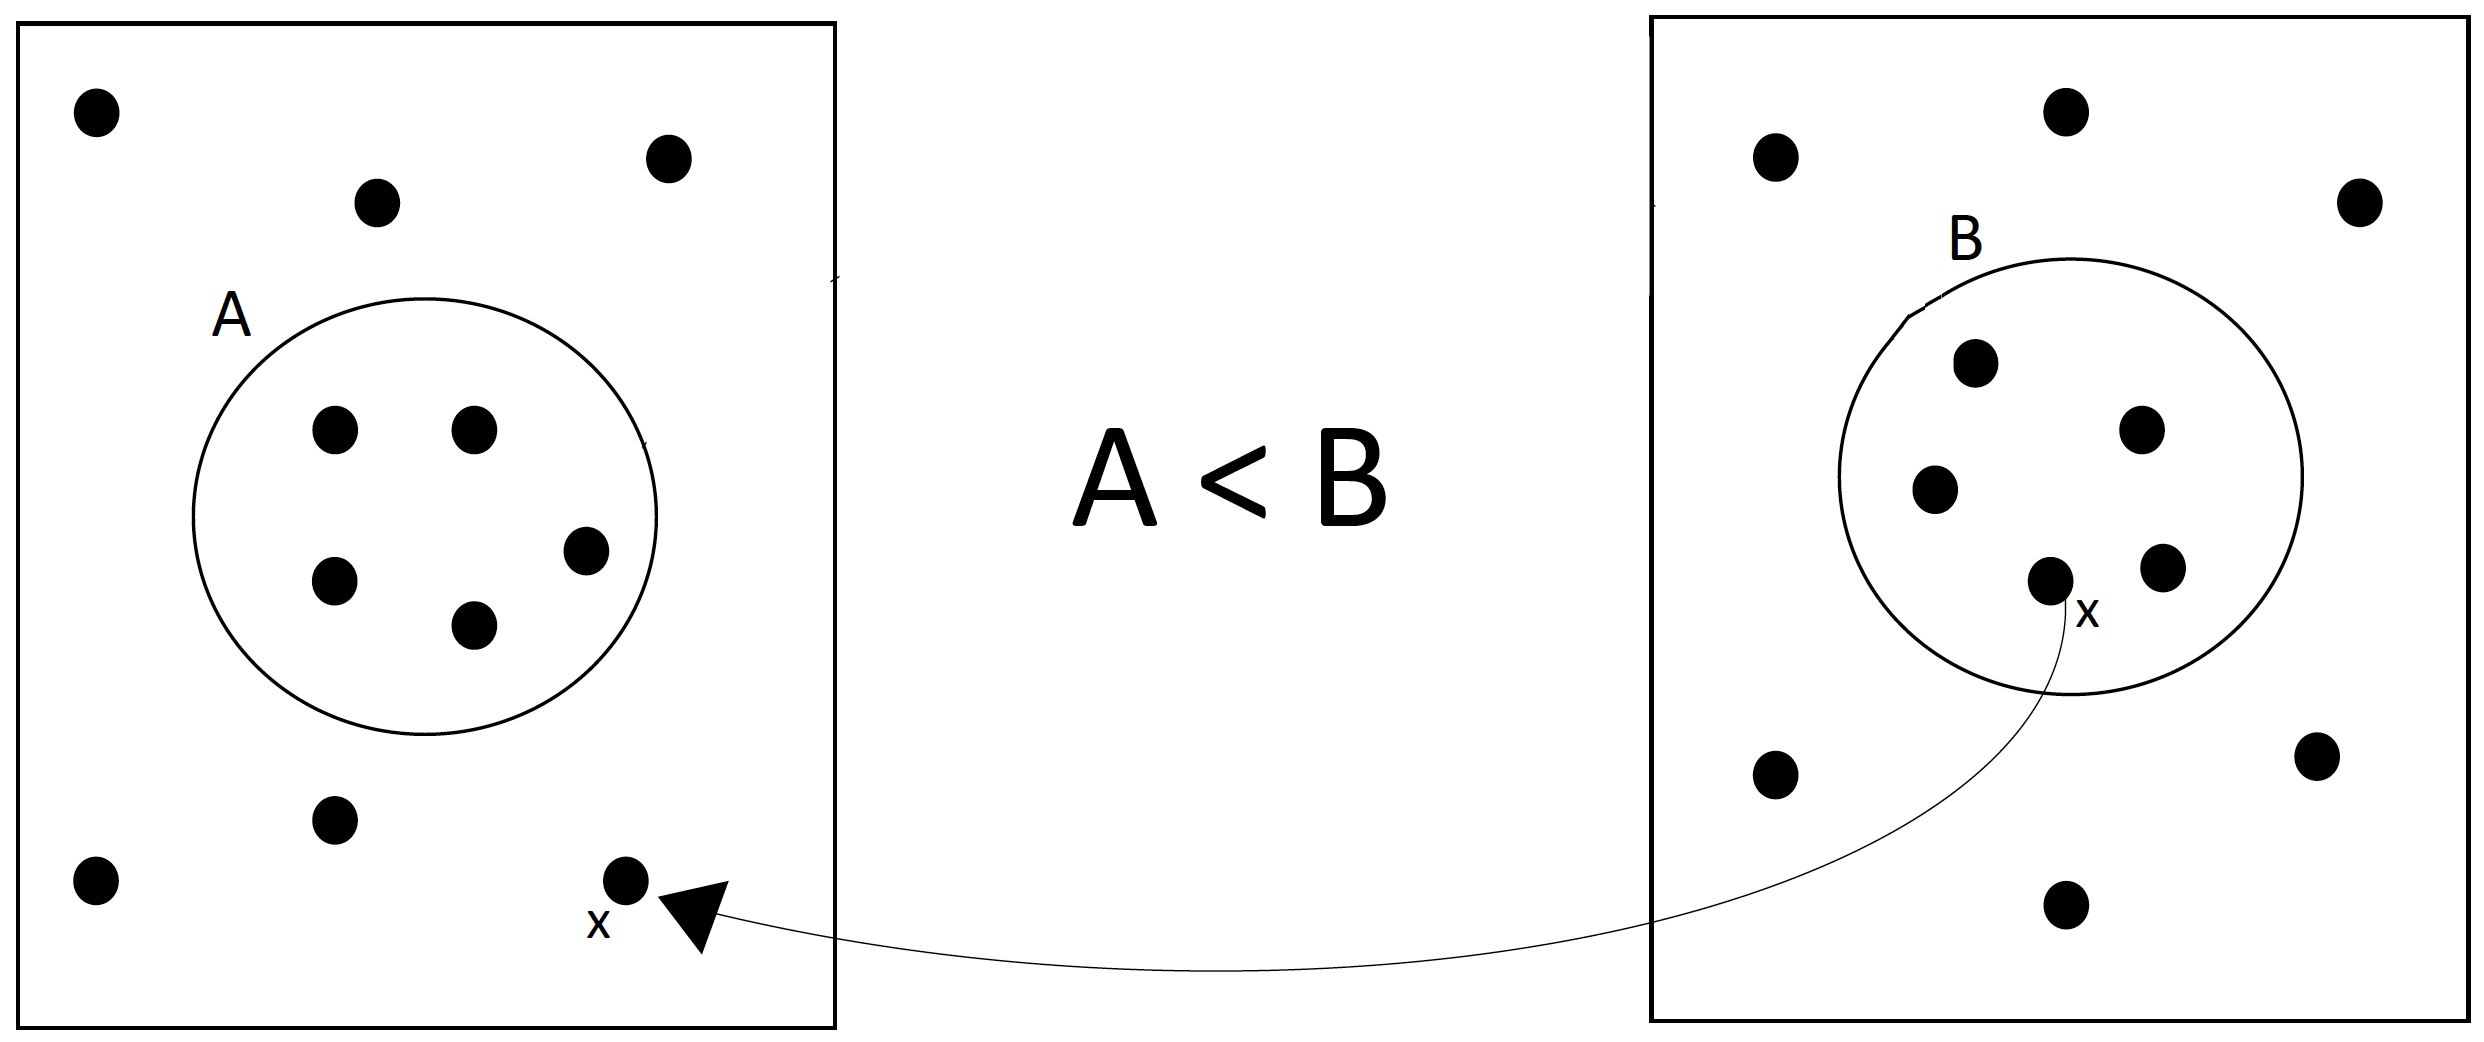
\includegraphics[width=0.9\textwidth]{less-set_2.png}}
   \only<4>{\hspace{-0.3cm}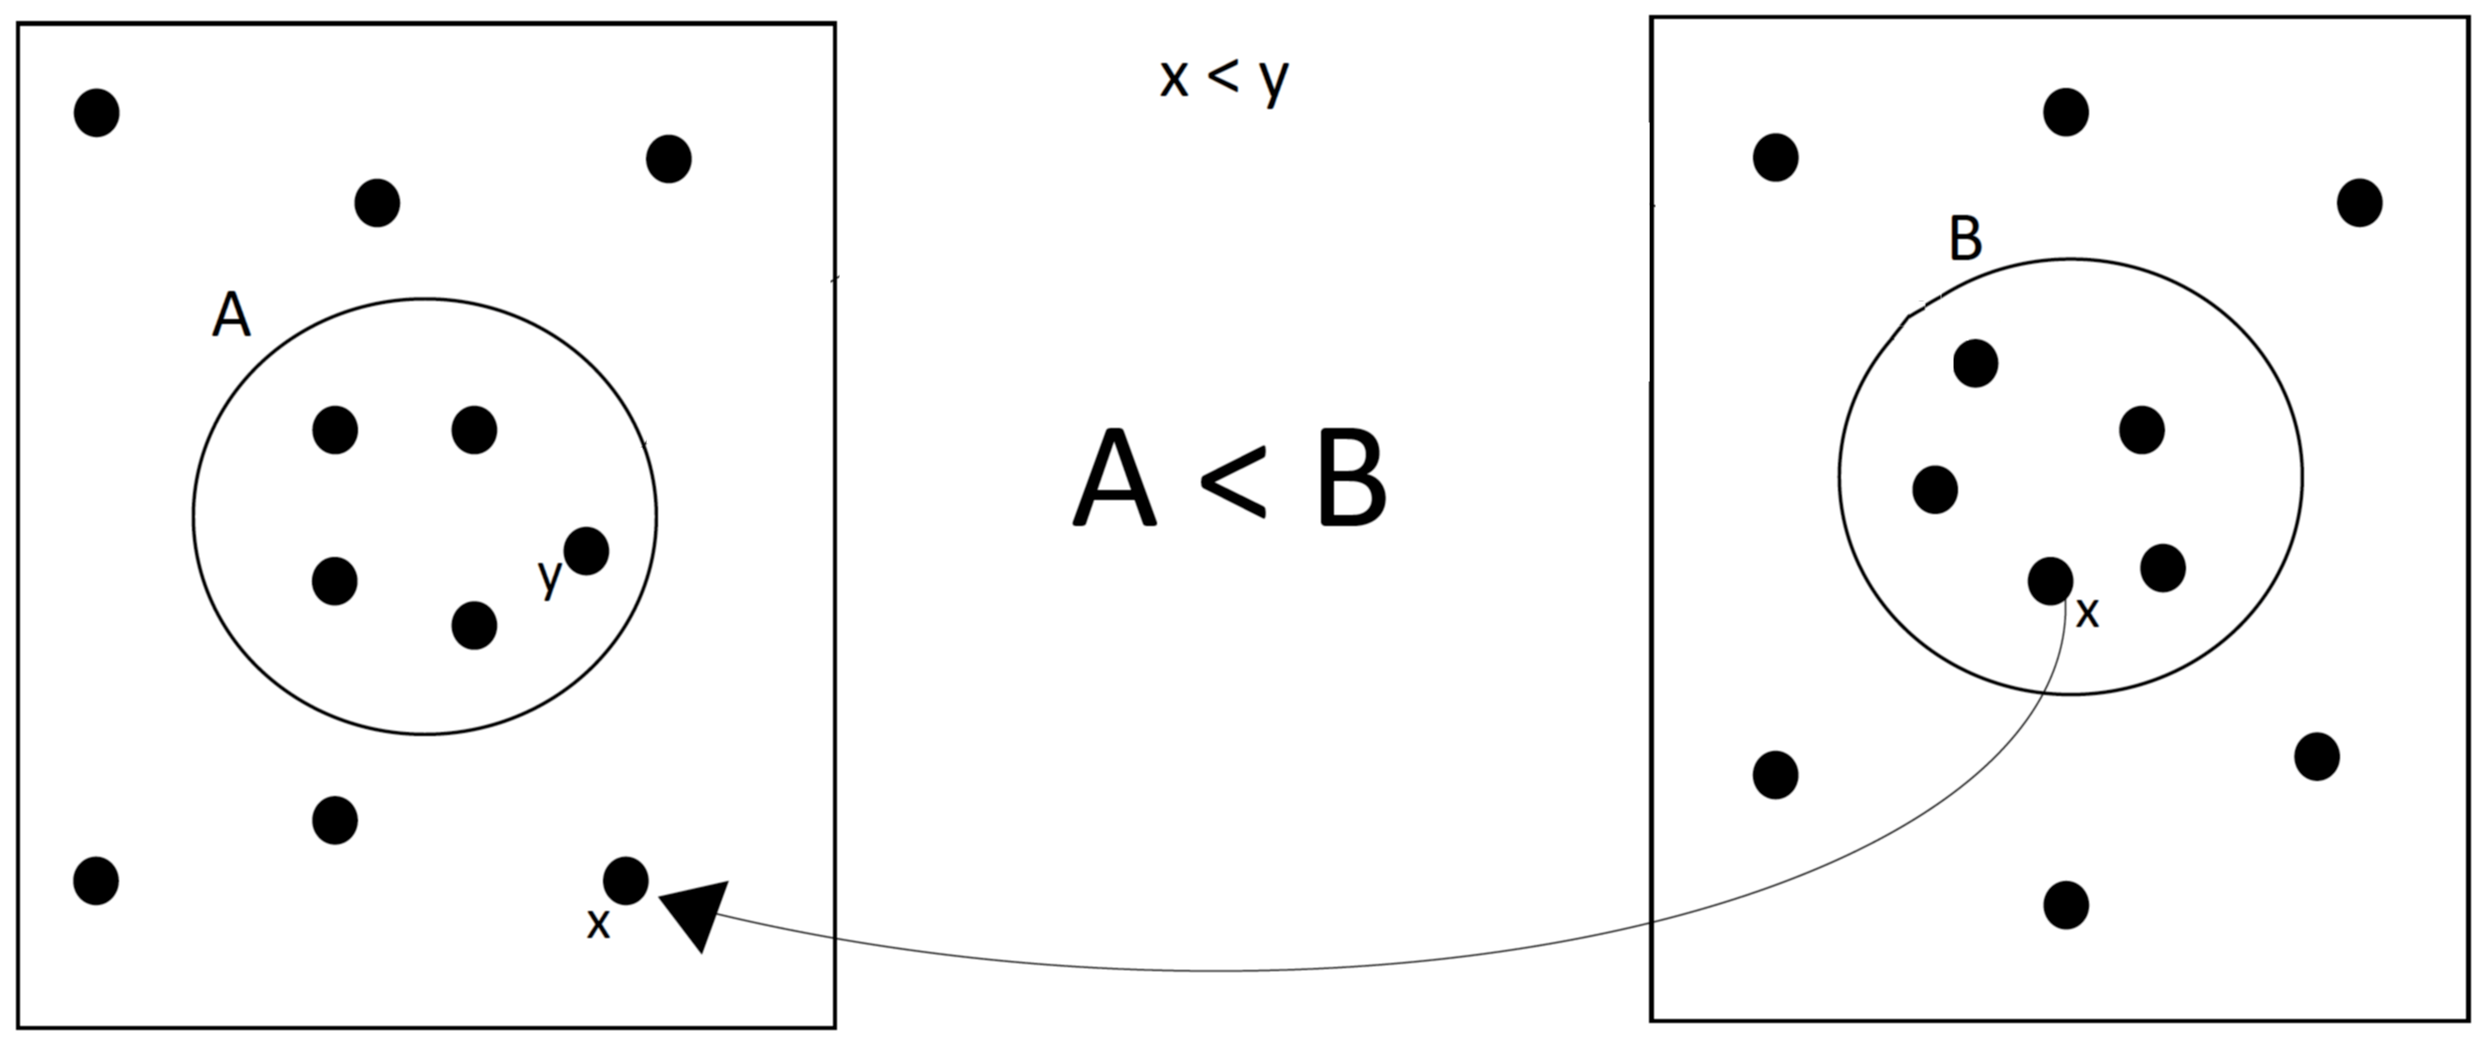
\includegraphics[width=0.9\textwidth]{less-set_3.png}}
  \only<5>{\hspace{-0.4cm}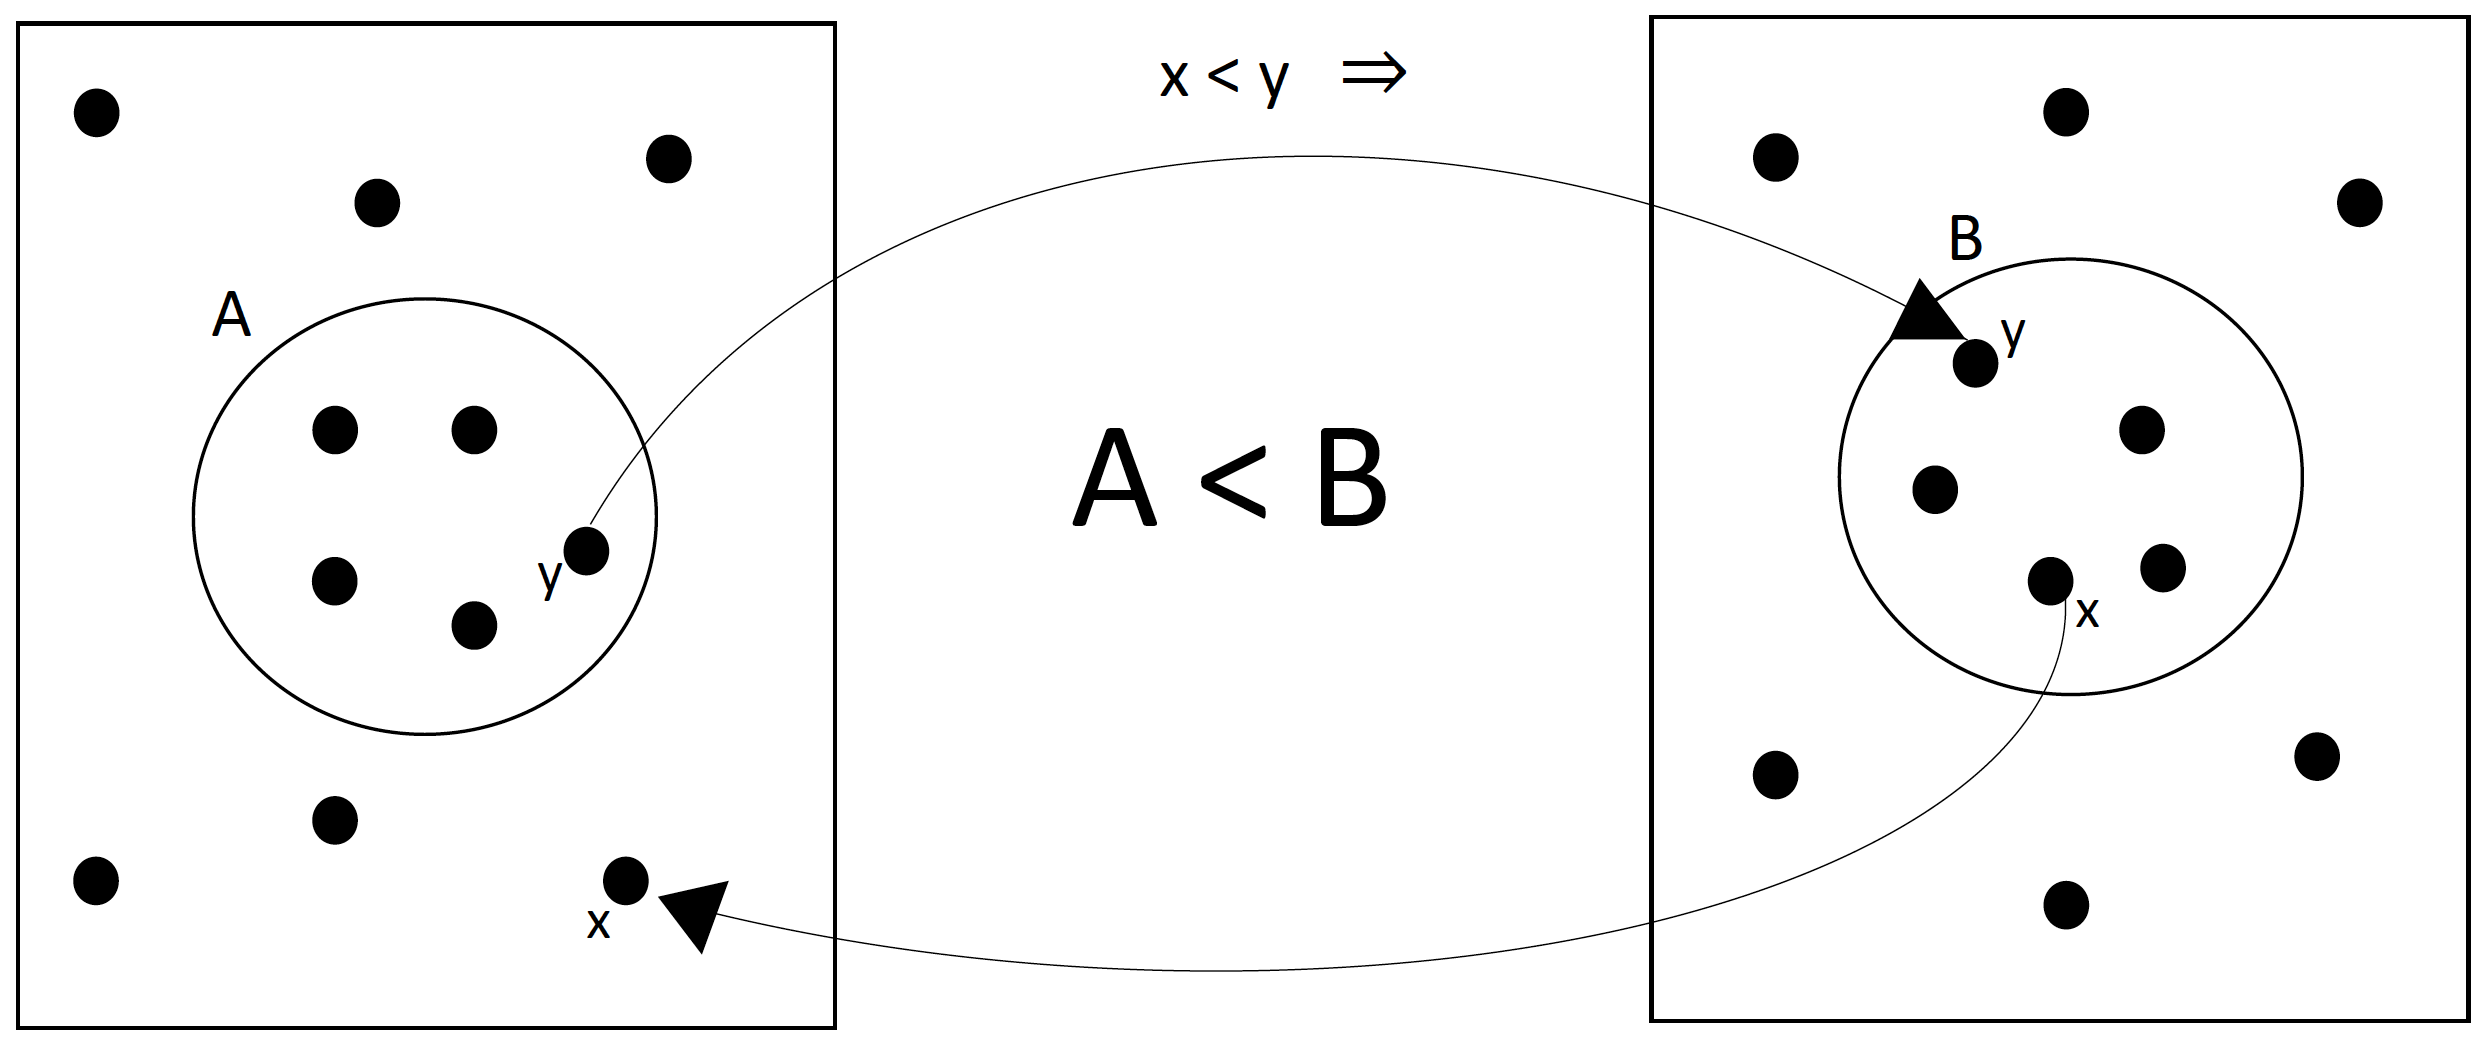
\includegraphics[width=0.9\textwidth]{less-set.png}}}
\end{figure}

\end{frame}
\begin{frame}

\begin{figure}[ht]
	\centering
  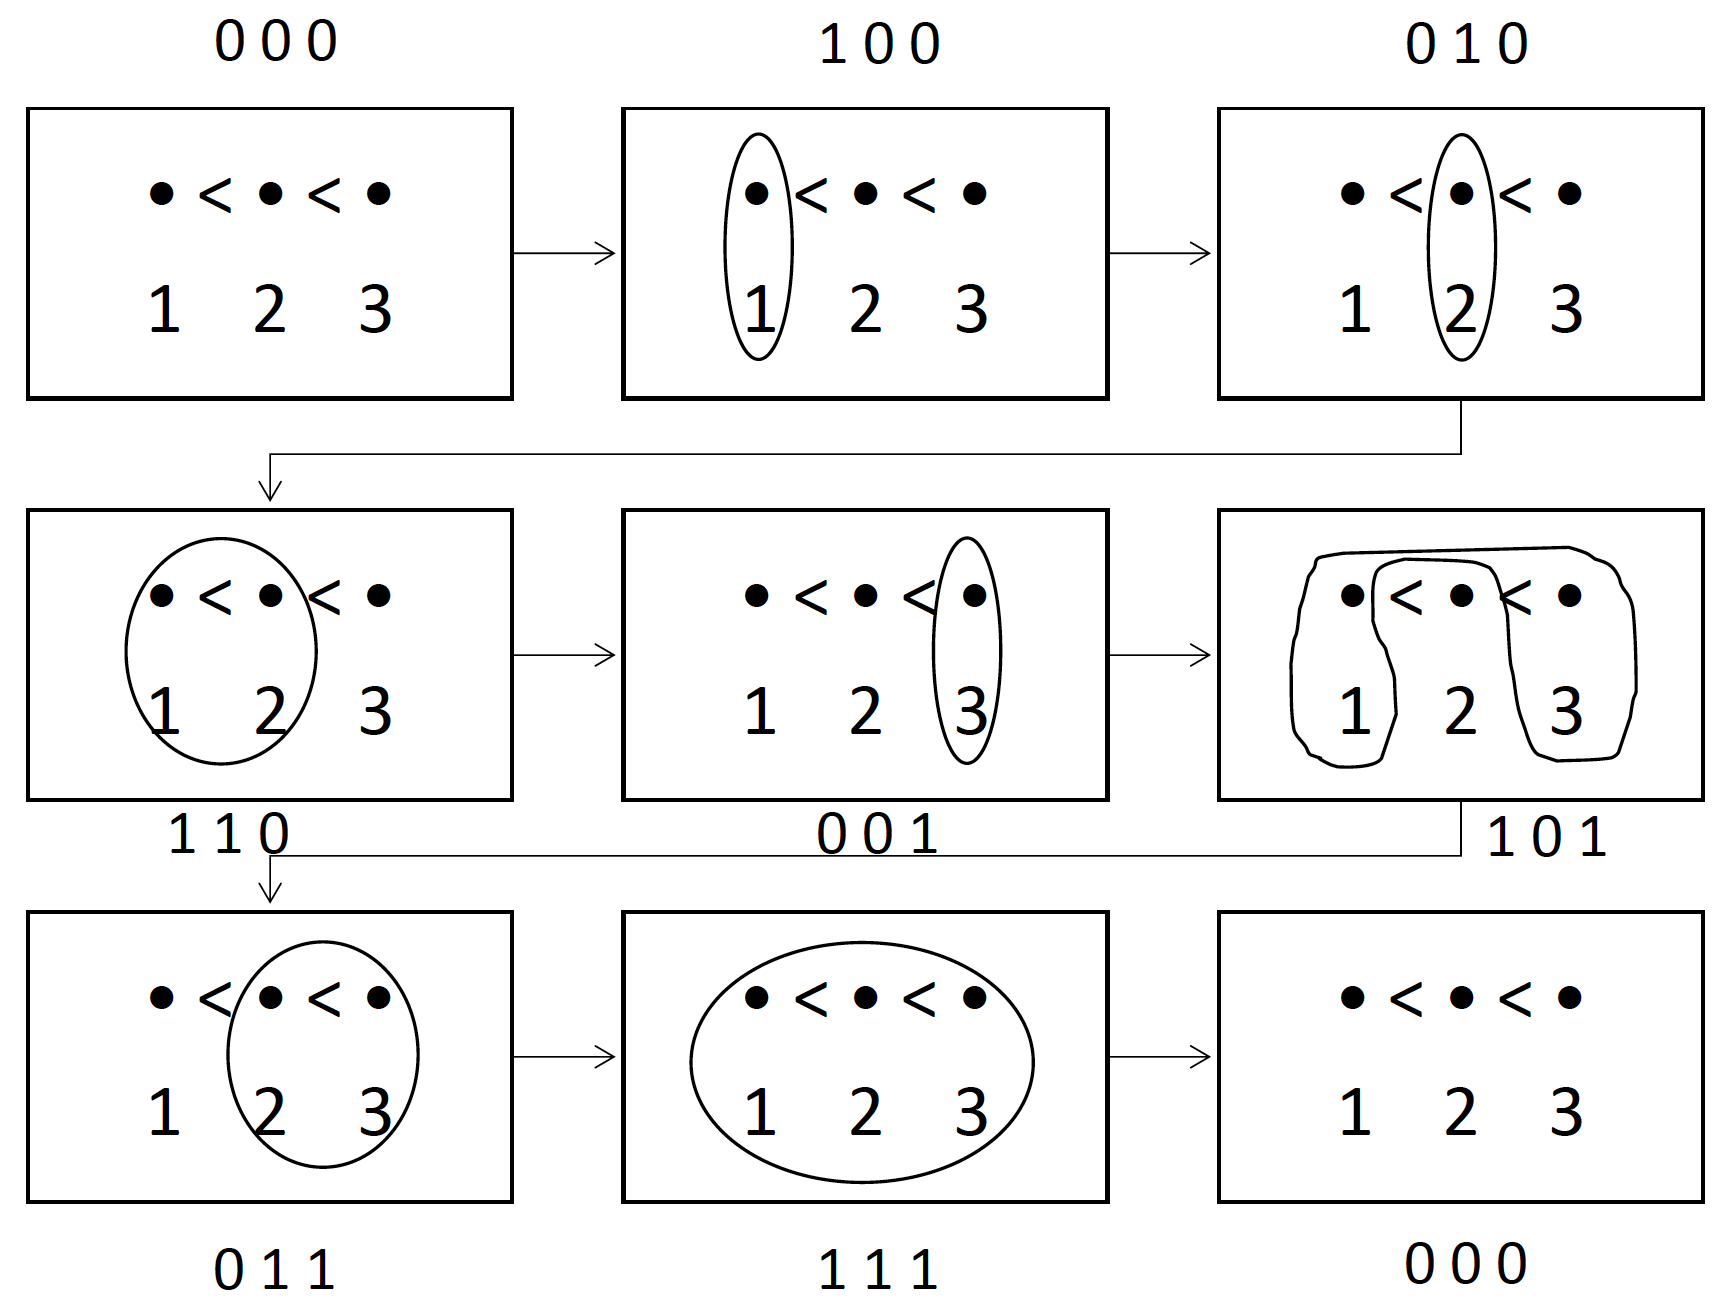
\includegraphics[width=0.9\textwidth]{next-set.png}
\end{figure}

\end{frame}
\begin{frame}

    \begin{align*}
        next^{(\tau, \dots, \tau)} \coloneqq &\,\lambda (X \colon T ((\tau, \dots, \tau))).\,\lambda (X_1 \colon T(\tau)).\, \dotsb \lambda (X_n \colon T(\tau)).\, \\&\,
        \big(\neg (\dotsb(X\,X_1)\dotsb)\,X_n \wedge \forall^{\tau}Y_1.\, \dots \forall^{\tau}Y_n.\,\\&\,<^{\tau \times
        \dots \times \tau}(Y_1, X_1, \dots, Y_n, X_n) \Rightarrow  (\dotsb(X\,Y_1)\dotsb)\,Y_n\big) \,\vee
        \\&\,\big((\dotsb (X\,X_1) \dotsb)\,X_n \wedge \exists^{\tau}Y_1.\, \dots \exists^{\tau}Y_n.\, \\&\,
        <^{\tau \times \dots \times \tau}
        (Y_1, X_1, \dots, Y_n, X_n)\,\wedge \neg (\dotsb(X\,Y_1)\dotsb)\,Y_n\big)
    \end{align*}

\end{frame}
\begin{frame}

    \begin{align*}
        \big(\mu (F \colon T(\tau') \rightarrow \bullet).\, \lambda (X \colon T(\tau')).\,
        \Phi(X)
        \vee F(next^{\tau'} X)\big)\bot_{T(\tau')}
    \end{align*}    
    \onslide<2-> is equivalent to
    \onslide<3->{ \begin{align*}
        \Phi(\bot_{T(\tau')})\, \vee 
        \Phi(next^{\tau'} \bot_{T(\tau')})\, \vee 
        \Phi(next^{\tau'} next^{\tau'} \bot_{T(\tau')}) \vee \dotsb.
    \end{align*} }   
    \onslide<4-> {This can be simplified to
    \[\underset{i\geq0}{\bigvee} \Phi({next^{\tau}}^i \bot_{T(\tau')}).\]}

\end{frame}

\section{Results}

\begin{frame}

\begin{theorem}
    Let $k \geq 0$. PHFL$^k$ captures \exptime{$k$} over finite labelled transition systems.
\end{theorem}

\begin{theorem}
    Let $k \geq 0$. PHFL$^{k+1}_{tail}$ captures \expspace{$k$} over finite labelled transition systems.
\end{theorem}

\end{frame}